\documentclass{report}

% match packages
\usepackage{amsmath}
\usepackage{xfrac}
\usepackage{breqn}  %line breaking for equations

% \usepackage{enumerate}
\usepackage{fixltx2e}
\usepackage[shortlabels]{enumitem}
\setlist{nosep}

\usepackage[left=1.5in, right=1in, top=1in, bottom=1in, includefoot, headheight=13.6pt]{geometry}

\usepackage{xcolor}
\usepackage{sectsty}
\chapterfont{\color{cyan}}  % sets colour of chapters
\sectionfont{\color{cyan}}  % sets colour of sections
\subsectionfont{\color{cyan}}
\subsubsectionfont{\color{cyan}}

% Package and setting for including pictures
\usepackage{graphicx}
\graphicspath{ {./Image/} }
\usepackage{caption}
\usepackage{subcaption}

% Packages for tables
\usepackage{tabularx}	%limiting table width
\usepackage{multirow}
\usepackage{booktabs}

% Package for generating dummy text
\usepackage[english]{babel}
\usepackage{blindtext}

% Package and Settings for table of contents
% Hyperlink Settings
\usepackage{hyperref}
\hypersetup{colorlinks, citecolor=black, filecolor=black, linkcolor=black, urlcolor=black}
% Settings for depth of table of contents
\setcounter{tocdepth}{3}
\setcounter{secnumdepth}{3}

%Package for creating appendix
\usepackage[toc,page]{appendix}

% Packages for citing and reference
\usepackage[backend=bibtex]{biblatex} 

% Packages for plotting
\usepackage{pgfplots}
\pgfplotsset{compat=1.8}
\usepgfplotslibrary{fillbetween}  
\usetikzlibrary{graphs} 
\usepackage{tikz}
% some tikz style defining
\usetikzlibrary{arrows,positioning} 
\tikzset{
    %Define standard arrow tip
    >=stealth',
    %Define style for boxes
    punkt/.style={
           rectangle,
           rounded corners,
           draw=black, very thick,
           text width=3.37cm,
           minimum height=2em,
           text centered},
    % Define arrow style
    pil/.style={
           ->,
           thick,
           shorten <=2pt,
           shorten >=2pt,}
}


% Packages for including code lines
\usepackage{listings}

% Define command for keyword in abstract
\providecommand{\keywords}[1]{\textbf{\textit{Keywords:---}} #1}

\bibliography{ref} 

\begin{document}

%!TEX root = first try.tex

\begin{titlepage}
    \begin{center}
        \vspace*{1cm}
        
        \textbf{\textcolor{cyan}{Background study and analytical model for railway bridge lateral dynamics}}
        
        \vspace{0.5cm}
        study of dynamics of railway bridges and applicability assessment of simplified dynamic analysing method.
        
        \vspace{1.5cm}
        
        \textbf{\textcolor{cyan}{Sijian Deng}}
        
        \vfill
        
        A thesis presented for the degree of\\
        Master of Science
        
        \vspace{0.8cm}
        
        % 
\includegraphics[width=0.4\textwidth]{TU_d_line_P1_color_1.jpg}
        
        % 
\includegraphics[width=0.4\textwidth]{Iv-Infra.jpg}

        \begin{figure}[h]
        \centering
        \begin{subfigure}[b]{0.3\textwidth}
                
\includegraphics[width=\textwidth]{TU_d_line_P1_color_1.jpg}
        \end{subfigure}
        \begin{subfigure}[b]{0.3\textwidth}
                
\includegraphics[width=\textwidth]{Iv-Infra.jpg}
        \end{subfigure}
        \end{figure}

        \begin{tabular} {cc}
        Faculty of Civil Engineering and Geo-science & Iv-Infra \\
        Delft University of Technology & Iv-Groep\\

        \end{tabular}

        The Netherlands \\
        \today
        
    \end{center}
\end{titlepage}

\begin{abstract}


Dynamics of railway bridges is a complicated problem that normally needs numerical simulation to conduct researches. However, this thesis takes advantage of the numerical results provided in D181 reports and based on these results, further conclusions are made by using them in analytical model. 

Recently long span railway bridges being designed in the Netherlands are being rejected by a particular EN1991-2 criterion that requires bridges to possess a first lateral natural frequency higher than 1.2Hz. Due to the fact that generally bridge's first lateral natural frequency decreases as the span increases, it can be seen that 1.2Hz criterion is rejecting almost all bridge with a span longer than 100m. 

This report succeeds in pursuing the original documents of 1.2Hz criterion and thes knowledge in the documents initiates further researches on the lateral dynamics of railway bridges. Besides 1.2Hz criterion itself, following topics are researched with the information provided by D181 report series:

\begin{enumerate}
    \item Two train-bridge lateral resonance mechanisms, including axle repeat pattern resonance and kinematic movement resonance,
    \item Lateral force on tracks caused by the operation of railway vehicle and key parameters influencing the force,
    \item Lateral wavelength of trains running in the Netherlands, including axle repeat pattern wavelength and kinematic movement wavelength
\end{enumerate}
    
Taking advantage of the items above, a practical method for checking the lateral railway bridge dynamics is developed to quantify the lateral dynamic resonance response of railway under horizontal dynamic vehicle load. This method aims to serve for engineering purposes and provide an alternative way of verifying railway bridge lateral dynamics other than 1.2Hz criterion. The practical method is developed by an analytical approach, based on the VAMPIRE simulation results in D181 DT329.

Once the exact expression for practical method has been obtained, an illustration of the usage of the practical method is conducted on the basis of a real bridge project. The method is also implemented in Matlab scripts to automate the checking procedure.

\vspace*{1cm}

\keywords{Eurocode, D181, railway bridge dynamics, lateral dynamics, rail dynamics, analytical solution, 1.2Hz criterion, train wavelength, nosing force, lateral force on track}

\end{abstract}




\chapter*{Acknowledgements}

Hereby I would like to express my deepest appreciation to all those who helped me in completing this thesis and my engineering studies.

First of all, I would like to thank to Matthijs van Almen, my daily supervisor at Iv-Infra, for his patient guidance during the entire thesis process. His guidance is like the light that helps me finding the right path in the darkness. Nevertheless, his way of thinking also enlightened me. I would never have completed the thesis without his help. 

I also want to express my appreciation to Prof. Frans Bijaard, Dr. Roland Abspoel, Dr. Micha{\"e}l Steenbergen, Prof. Rolf Dollevoet,  the members of the thesis committee from Delft University of Technology. Their professional knowledge and general interest in the topic were valuable assets to my work.

Special thanks to Michel Koop, who provided me with the opportunity to carry out this research at Iv-Infra, to Charalampos Bouras, who was always eager to provide help whenever I needed, and to all the colleagues at the steel department of Iv-Infra, who provided me a friendly atmosphere.

I really appreciate the help of Ron van der Zwan and the access to ERRI D181 research resources he provided. I also appreciate Paul Vos, Jean-Jacques Reber sharing their background information of D181 committee. Same appreciation goes to Alan Minnis from DeltaRail for providing the information of D181 DT329 researches.

Thanks to  the contributors of both StackOverflow who generously sharing the knowledge and {\LaTeX} for maintaining such an incredible package. 

I am deeply grateful to my parents, Guolin Deng and Jiafen Wang, who always believed in me and were supporting my studies in The Netherlands. 

Last but not least, I am thankful to all my friends in Delft, who gave me many unforgettable memories during my studies.

\vspace*{1cm}

Sijian Deng

Delft,  \today


\tableofcontents

%!TEX root = first try.tex

\chapter{INTRODUCTION}

\section{Summary of topic}

The lateral dynamic behaviour of steel railway bridges are minimally discussed in Eurocodes and designers lack knowledge of background of criteria proposed in the code. For example, there is one criterion in Eurocode requiring railway bridges should have a lateral natural frequency higher than 1.2Hz. However, this criterion is becoming more and more unsuitable because longer span provides lower natural frequencies. For bridges having span more than 100m, it is almost guaranteed that the first lateral natural frequency of the bridge fall below 1.2Hz, unable to meet the requirement of Eurocode. 

Criteria on lateral dynamics of railway bridges are complicated if taking vehicle systems and interaction into account. Designers need a better knowledge on railway dynamics and a tool in calculating the lateral dynamic behaviour of the whole system. This tool needs to be simple to meet the engineering needs.  

\section{Motivation of the thesis}


\section{Objectives and research question}\label{sec:introduction}

The main goal is to think of a method to verify whether a bridge is expected to encounter transverse dynamic problems. 

In the literature study the criteria of different systems involved in dynamic response of steel railway bridges will be investigated. Governing criteria will be selected into an inventory. The criteria inventory is useful by providing what to represent in simplified model. 

The simplified model will be developed based on real train information in order to natively support Dutch designers. The result simplified model output shall be in cooperation with the criteria inventory made in previous steps.

Using the developed model and the knowledge of literature study, an imaginary steel railway bridge can be designed, in order to verify the reliability of the newly developed tool. 

\section{Main steps}

In order to provide a better tool for designers when they encounter lateral dynamic problems on steel railway bridges, following objectives are made:

\begin{enumerate}

\item Literature research of dynamic actions as well as their criteria on railway bridges, rails and train vehicles in order to give a better understanding of the background of the criteria which is unclear to the designers. Study the dynamic behaviour of these system respectively. Then discuss their effects when combined.

\item Develop a method to check if a bridge is prone to encounter dynamic problems. The method should be simple. It should be compatible with FEM software and give suggestions for further bridge modification. However form of the method will depend on output of the literature research.

Several forms of method have been made and will be illustrated during kick-off presentation.

\item Verify the model developed in the previous step by checking a long-span railway bridge. 

\end{enumerate}

\section{Research methodology}
\section{Outline of the report}



%!TEX root = first try.tex  

\chapter{LITERATURE REVIEW} 
Eurocode 1990 and Eurocode 1991-2 and their corresponding National Annex are primary codes to be fulfilled through out the whole process of conducting a railway bridge in Netherlands. It is of great importance to study dynamic effect on railway bridges due to increasing usage of public train service. What's more, as the need on capacity of railway service increase, high-speed train dynamic loading becomes a more general issue in the design of railway bridges. It is common knowledge that bridge structures loaded by high-speed trains have bigger chance of resonance, as well as of being required to be dynamic analysed in designing process. 

Unfortunately in Chapter 6.4 of Eurocode NEN-EN 1991-2-2003, the description of various subjects is vague including general procedures of conductinga dynamic analyses and methods of additional dynamic analysing calculating, etc. The following paragraphs aim to summarize Chapter 6.4 of Eurocode 1991-2 \cite{EC12}, in order to give a better interpretation. 

This literature research will be done by reviewing both physics knowledge and engineering standards.

\section{Forced Vibrations under Harmonic Force}
Assume there is a simple one degree-of-freedom mass-spring system and an external force is acting on it. The force is given as $F(t)= F_0 \cos(\omega t)$. In this case the equation of motion takes the form
\begin{equation}
	m\ddot{x} + kx = F_0 \cos(\omega t)
\end{equation}

The general solution can be written as
\begin{equation}
	x(t) = A\cos(\omega_n t)+B\sin(\omega_n t) +\frac{F_0}{k}\frac{1}{1-\omega^2/\omega_n^2}\cos(\omega t)
\end{equation}

The unknown constants A and B depend on the initial conditions.

The steady-state solution is given as:

\begin{equation}
	x_{steady}= X \cos(\omega t) = \frac{F_0}{k}\frac{1}{1-\omega^2/\omega_n^2}\cos(\omega t)
\end{equation}

The amplitude of vibrations of the mass-spring system is given by:
\begin{equation}
	|X|=|\frac{F_0}{k}\frac{1}{1-\omega^2/\omega_n^2}|
\end{equation}

The amplitude-frequency dependencies is shown in \ref{fig:amplitude-frequency-characteristic} 

\begin{figure}[h]
	\centering
	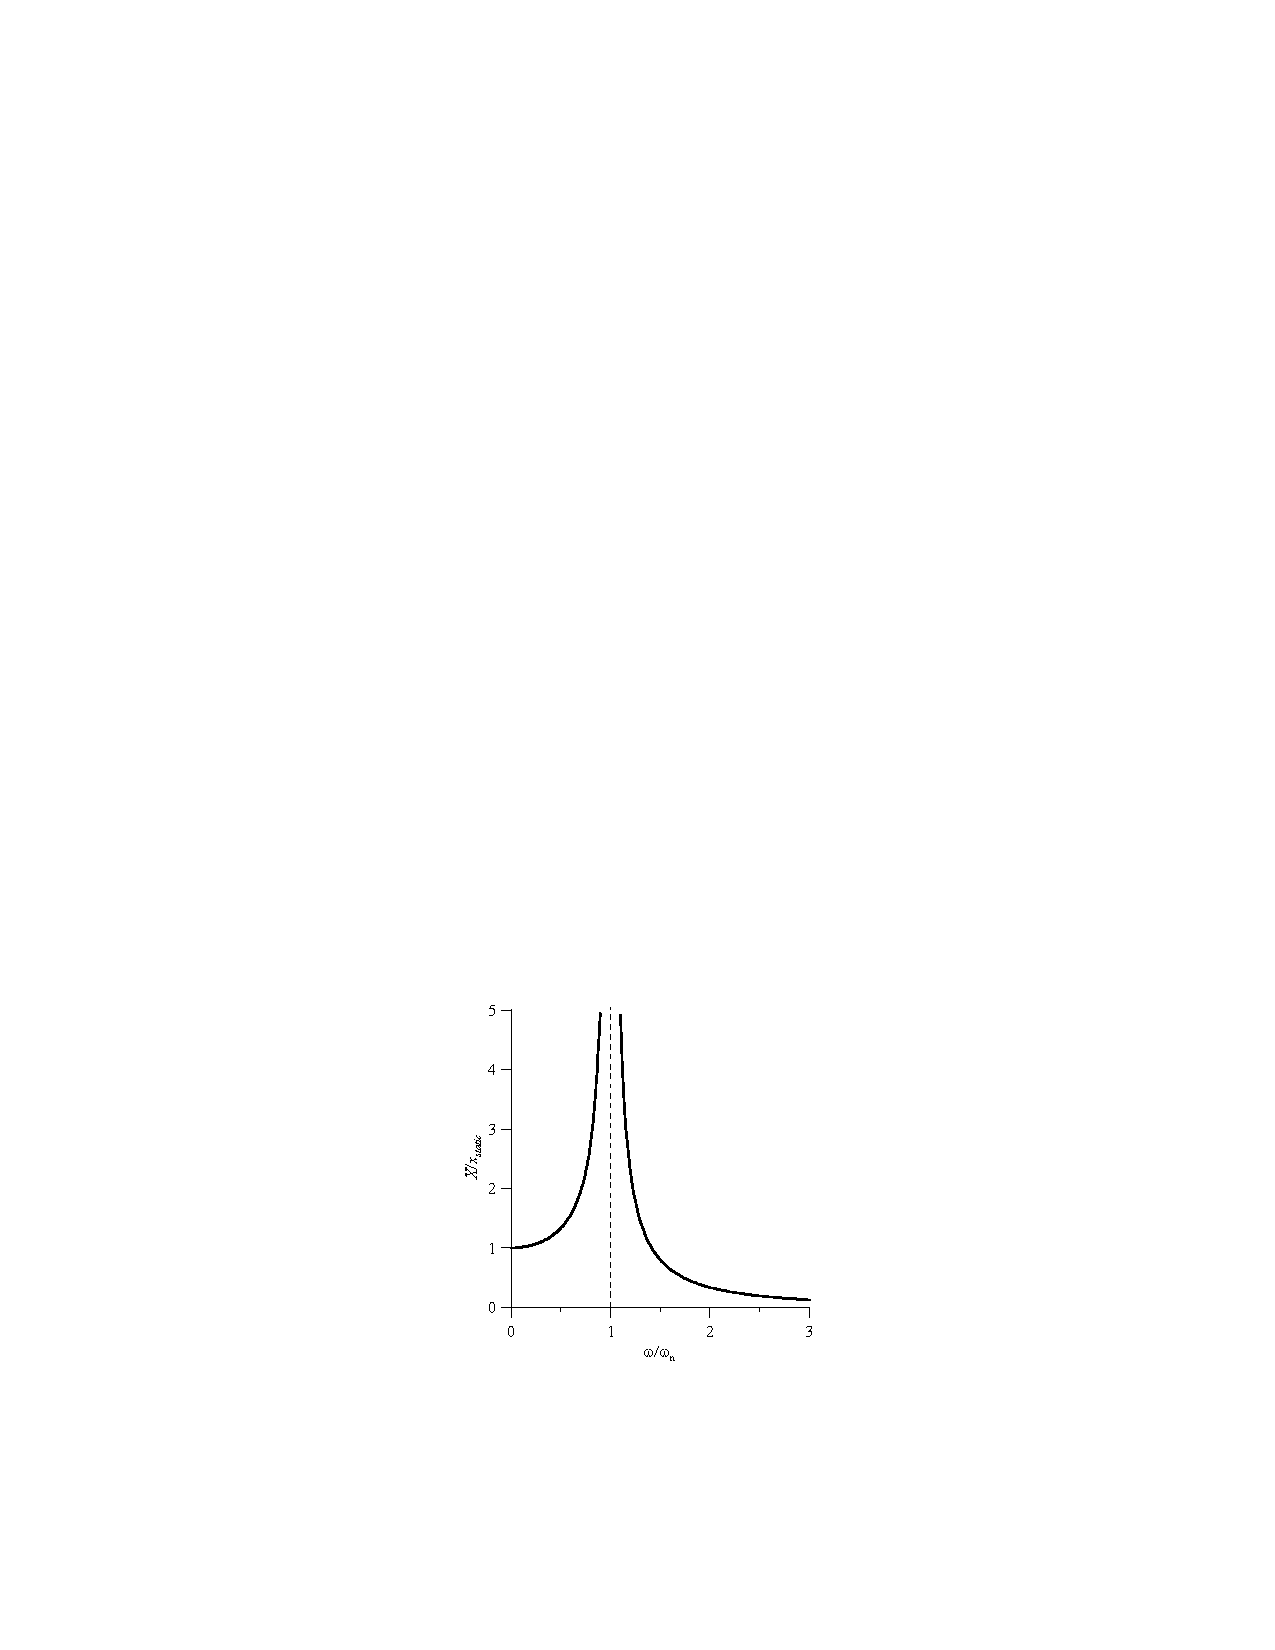
\includegraphics[width=0.6\textwidth]{amplitudefrequencycharacteristic.pdf}
	\caption{Amplitude-frequency characteristic. Extracted from \cite[2.2.2]{dynamicslecturenote}}
	\label{fig:amplitude-frequency-characteristic}
\end{figure}


\section{Introduction to the dynamics of railway bridges}

\cite{fryba1996dynamics}Dynamics of railway bridges is concerned with the study of deflections and stresses in railway bridges. The loads are represented by the moving wheel and axle forces, by means of which railway vehicles transmit their load and inertia actions to railway bridges. A survey of the dynamic effects of vehicles on railway bridges is given in Figure.\ref{fig:dynamic effects}

\begin{figure}[h]
	\centering
	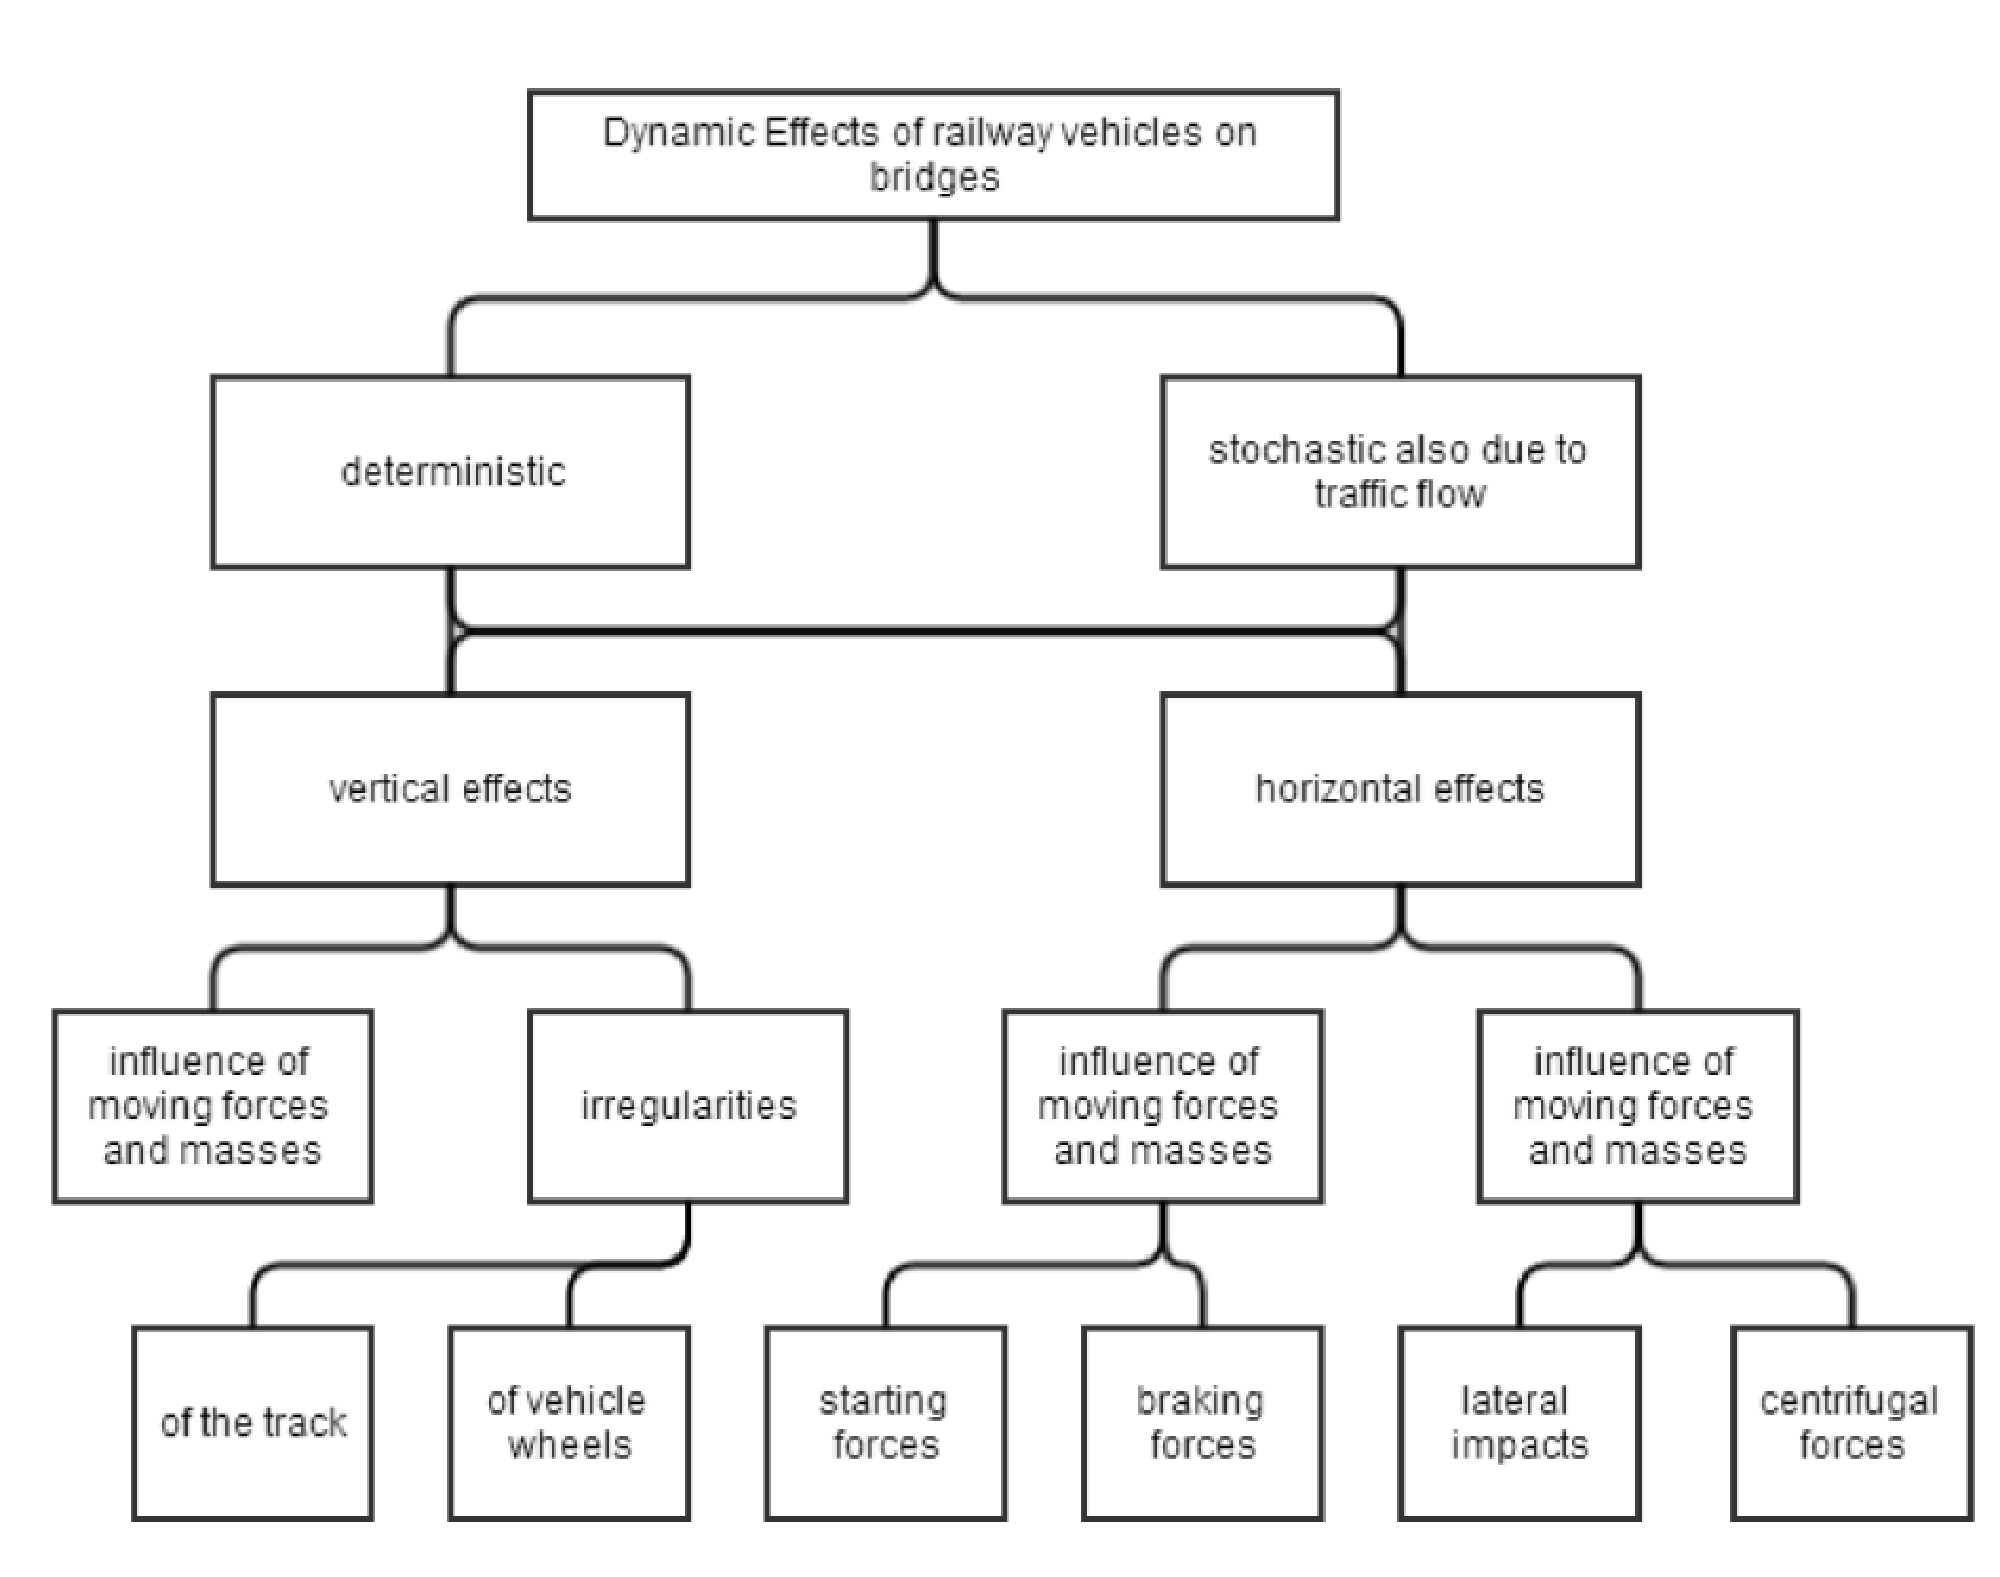
\includegraphics[width=0.6\textwidth]{dynamiceffects.pdf}
	\caption{Dynamic effects of railway vehicles on bridges. Extracted from \cite[1.1]{fryba1996dynamics} }
	\label{fig:dynamic effects}
\end{figure}

\subsection{Factors influencing dynamic behaviour}
As stated in\cite[6.4.2]{EC12} there are 11 factors influencing dynamic behaviour of a railway bridge. The principal factors which influence dynamic behaviour are:
\begin{enumerate}[-]
	\item the speed of traffic across the bridge
	\item the span L of the element and the influence line length for deflection of the element being considered
	\item the mass of the structure
	\item the natural frequencies of the whole structure and relevant elements of the structure and the associated mode shapes (eigenforms) along the line of the track
	\item the number of axles, axle loads and the spacing of axles
	\item the damping of the structure
	\item vertical irregularities in the track
	\item the unsprung/sprung mass and suspension characteristics of the vehicle
	\item the presence of regularly spaced supports of the deck slab and/or track (cross girders, sleepers etc.)
	\item vehicle imperfections (wheel flats, out of round wheels, suspension defects etc.)
	\item the dynamic characteristics of the track (ballast, sleepers, track components etc.)
\end{enumerate}

Other factors may include:

\begin{enumerate}

	\item The track number of the bridge and their alignment. 
	\item Multiple trains running on bridge simultaneously. 
	\item Track alignment

\end{enumerate}



\section{Vertical Dynamic effects}
As stated in EN 1991-2\cite{EC12}, the static stress and deformations (and associated bridge deck acceleration) induced in a bridge are increased and decreased under the effects of moving traffic by the following:

\begin{enumerate}[-]
	\item the rapid rate of loading due to the speed of traffic crossing the structure and the inertial response (impact) of the structure,
	\item the passage of successive loads with approximately uniform spacing which can excite the structure and under certain circumstances create resonance (where the frequency excitation(or a multiple there of) matches a natural frequency of the structure (or a multiple there of), there is a possibility that the vibrations caused by successive axles running onto the structure will be excessive),
	\item variations in wheel loads resulting from track or vehicle imperfections (including wheel irregulations).
\end{enumerate}
For determining the effects (stresses, deflections, bridge deck acceleration etc.) of rail traffic actions the above effects shall be taken into account.


\subsection{Train Actions}
See section \ref{designprocedures}


\subsection{Wind Actions}
The nature of the wind load is dynamic. This means that its magnitude varies with respect to time and space.

According to \cite{mohammadi2013wind}: The limitations behind the applications of the EN-1991-1-4, Eurocode1, actions on structures-general actions-wind load-part 1-4, lead the structural designers to a great confusion. This may be due to the fact that, EC1 provides only the guid- ance for the bridges whose fundamental mode of vibrations have constant sign (e.g. simply supported structures) or a simple linear sign (e.g. cantilever structures) and these modes are the governing mode of vibrations of the structure; it analyzes only the along-wind response of the structure and not the cross wind response and the simplified methods recommended in this code are covering only the structures with simple geometrical configurations.

\section{Horizontal transverse dynamic effects}
There's only one criterion in the Eurocodes mentioned that the bridge's first lateral natural frequency should no lower that 1.2 Hz. Dynamic analyses are required if this criterion is not met. 

However, as more and more long-span bridges are built nowadays, this requirement is not valid for more bridges. This is because, in general, the lateral natural frequency of a bridge decreases when span increases. For bridges with span longer than 100m, there's few bridge can have a lateral frequency higher than 1.2Hz, according to senior engineers' designing experience.

So it is vital to discuss horizontal dynamic effects for the sake of longer span bridges. In additional, study the requirements for horizontal vibration of railway bridges to make the results of dynamic analysis usable.

\subsection{Sources induce transverse dynamic reactions}
According to \cite{da2007dynamic}\cite{fryba1996dynamics}\cite{EC12}, following sources are identified:

\begin{enumerate} [-]
	\item Horizontal track irregularities
	\item Sinusoidal motion of conical wheels along cylindrical rail heads
	\item Centrifugal forces on curved tracks
	\item Train switches
\end{enumerate}

\subsection{Horizontal vibration of a beam}

Fryba\cite{fryba1996dynamics} described the first two sources in mathematical terms:
Consider a simply supported beam loaded by moving train loading, horizontal vibrations of the beam in a transverse direction $ w(x,t) $ are generated by lateral random forces $ H_n (t) $ due to random irregularities and sinusoidal motion. The differential equation for the deformation is:

\begin{equation}
	EI_yw^{IV}(w,t)+\mu \ddot{w} (x,t)=\sum_{n=1}^{N} \varepsilon_n\delta(x+d_n-ct)H_n(t) 
\end{equation}

where $ H_n(t) $ stands for forces due to random irregularities and sinusoidal motion. $ H_n(t) $ is of a typically random character and can be replaced by horizontal transverse forces with zero mean values. See Figure.~\ref{fig:trackirrg} for example.

\cite[Table 9.1]{fryba1996dynamics} gives sample of natural frequencies of steel truss bridges with open deck. Shown as follow Table~\ref{tab:spatialvibrationsteel}. Please note that truss bridges have high stiffness.

\begin{table}[h]
	\centering
	\begin{tabular}{ccccc}
		\hline
		\multirow{2}{*}{Vibration Type} & \multirow{2}{*}{Symbol} & \multirow{2}{*}{j} & \multicolumn{2}{c}{Bridge with span} \\
		\cline{4-5}
		 & & & $ l=25.85m $ & $ l=48.4m $\\
		\hline
		\multirow{3}{*}{Vertical} & \multirow{3}{*}{$ f_j $} & 1 & 8.7 & 5.4\\
		 & & 2 & 34.7 & 21.5 \\
	 	 & & 3 & 78.1 & 48.3 \\
	 	\hline
	 	\multirow{9}{*}{Horizontal} & \multirow{3}{*}{$ f_{hj} $} & 1 & 15.3 & 4.7 \\
	 	 & & 2 & 61.1 & 19.0 \\
	 	 & & 3 & 137.5 & 42.7 \\
	 	\cline{2-5}
	 	 & \multirow{3}{*}{$ f_{yj} $} & 1 & 14.8 & 4.7 \\
	 	 & & 2 & 53.9 & 18.1 \\
	 	 & & 3 & 107.4 & 38.8 \\ 
	 	\cline{2-5}
	 	 & \multirow{3}{*}{$ {f}'_{yj} $} & 1 & 14.7 & 4.6 \\
	 	 & & 2 & 52.5 & 17.5 \\
	 	 & & 3 & 101.7 & 36.4 \\ 
	 	\cline{2-5}
	 	\hline
	 	\multirow{9}{*}{Torsional} & \multirow{3}{*}{$ f_{\xi j} $} & 1 & 35.7 & 19.2 \\
	 	 & & 2 & 71.3 & 38.4 \\
	 	 & & 3 & 107.0 & 57.7 \\
	 	\cline{2-5}
	 	 & \multirow{3}{*}{$ f_{\varphi j} $} & 1 & 34.9 & 16.7 \\
	 	 & & 2 & 73.5 & 35.4 \\
	 	 & & 3 & 117.4 & 56.9 \\ 
	 	\cline{2-5}
	 	 & \multirow{3}{*}{$ {f}'_{\varphi j} $} & 1 & 36.5 & 19.7 \\
	 	 & & 2 & 77.6 & 41.9 \\
	 	 & & 3 & 126.4 & 67.5 \\ 
	 	\hline
	\end{tabular}
	\caption{Spatial vibrations of steel truss bridges with open bridge deck}
	\label{tab:spatialvibrationsteel}
\end{table}


\begin{figure}[p]
	\centering
	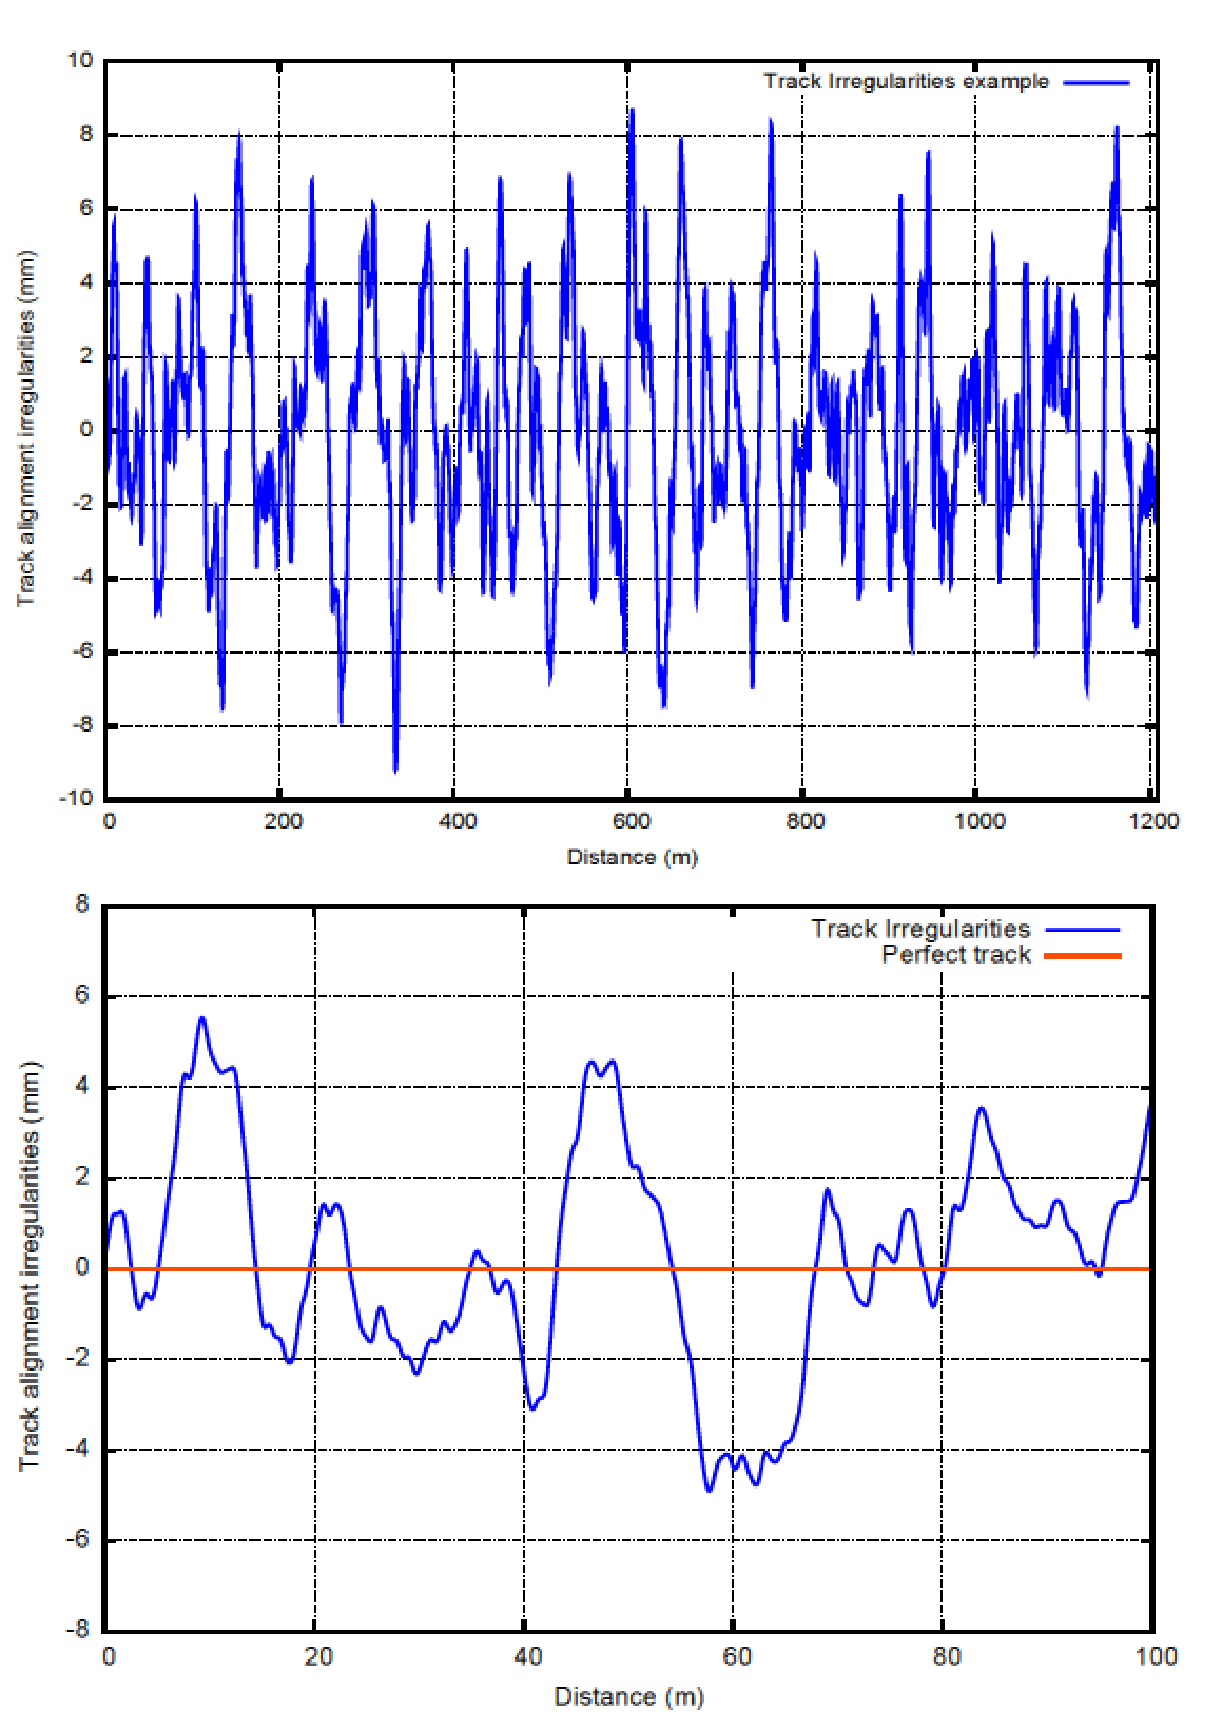
\includegraphics[width=0.8\textwidth]{trackirregularities.pdf}
	\caption{Example of a track lateral alignment irregularities profile for a track with low irregularities in a total length of 1209m.  Extracted from \cite{da2007dynamic}}
	\label{fig:trackirrg}
\end{figure}


\subsubsection{Centrifugal forces}
In \cite[6.5.1]{EC12} specifies following principles about centrifugal forces act on railway bridges:

Where the track on a bridge is curved over the whole or part of the length of the bridge, the centrifugal force and the track cant shall be taken into account.

The centrifugal forces should be taken to act outwards in a horizontal direction at a height of 1.80m above the running surface (see \cite[Figure 1.1]{EC12}). For some traffic types, e.g. double stacked containers, an increased value of $h_t$ should be specified.

The centrifugal force shall always be combined with the vertical load. The centrifugal force shall not be multiplied by the dynamic factor $\varPhi_1$ or $\varPhi_3$.

The characteristic value of the centrifugal force shall be determined according to the following equations:

\begin{equation}
	Q_tk=\frac{v^2}{g \cdot r}(f \cdot Q_{vk})=\frac{V^2}{127r}(f \cdot Q_{vk})
\end{equation}

\begin{equation}
	q_{tk}=\frac{v^2}{g \cdot r}(f \cdot q_{vk})=\frac{V^2}{127r}(f \cdot q_{vk})
\end{equation}

where:

\begin{tabular}{ll}
$Q_{tk}$,$q_{tk}$ & Characteristic values of the centrifugal forces\\
$Q_{vk}$,$q_{vk}$ & Characteristic values of the vertical loads specified in \cite[6.3]{EC12}\\
$f$ & Reduction factor, see below \\
$v$ & Maximum speed in accordance with \cite[6.5.1(5)]{EC12}[m/s]\\
$V$ & Maximum speed in accordance with \cite[6.5.1(5)]{EC12}[km/h]\\
$g$ & Acceleration due to gravity [9.81$m/s^2$]\\
$r$ & Radius of curvature [m].
\end{tabular}

For Load Model 71 (and where required Load Model SW/0) the reduction factor $f$ is given by:

\begin{equation}
	f=[1-\frac{V-120}{1000}(\frac{814}{V}+1.75)(1-\sqrt{\frac{2.88}{L_f}})]
\end{equation}

\subsection{Requirements for traffic safety(horizontal)}
Requirements other than bridge first lateral frequency higher than 1.2Hz. Since there's no further requirements mentioned by Eurocode, following requirements are gathered from other European codes, eg. British standards, UIC leaflet, etc.

\begin{enumerate}[-]
	\item Requirements regarding traffic safety for vehicles
	\begin{enumerate}
		\item Guiding Force: \cite{code2005518} , \cite{en200714363} and\cite{cuadrado2008analysis} propose safty limitations against railway vehicle overturning. From\cite{en200714363} the maximum guiding force for a vehicle with a load per axle of 170kN(AVE) is 66kN per axle and 48kN per axle for a vehicle with a load per axle of 112kN(ICE2). For the R1 freight wagon(load per axle of 245kN), the maximum guiding force per axle is 78kN.
		\item Maximum lateral acceleration of the railway vehicle: proposed by \cite{13803}
	\end{enumerate}
	\item Requirements regarding safety for bridge\\
	\cite{EC0} A2.4.4.1(2): Horizontal transverse deflection(to ensure acceptable horizontal track radii) and horizontal rotation of a deck about a vertical axis at ends of a deck(to ensure acceptable acceptable horizontal track geometry and passenger comfort)
\end{enumerate}


\subsection{Requirements for traffic safety on derailment: Railway vehicle derailment mechanism and safety criteria}

Derailment mechanisms
\begin{enumerate}
	\item vehicle resonant response
	\item lateral instability
	\item vehicle overturning
	\item vertical wheel unloading
	\item flange climb
	\item rail roll-over
	\item track panel shift
	\item longitudinal train forces
\end{enumerate}

The four types of derailment: flange climb derailment, derailment caused by guage widening and rail roll-over, derailment caused by track panel shift, derailment cause by vehicle lateral instability have a common cause of high lateral force at the wheel-rail interface. According to \cite[Chapter 8, IV]{iwnicki2006handbook} any conditions that lead to high lateral forces or lead to lower the ability of the system to sustain the force should be corrected. 

\subsubsection{Flange climb derailment}
Wheel flange climb derailments are caused by wheels climbing onto the top of the railhead then further running over the rail. Wheel climb derailments generally occur in situations where the wheel experiences a high lateral force combined with circumstances where the vertical force is reduced on the flanging wheel. The high lateral force is usually induced by a large wheelset angle-of-attack. The vertical force on the flanging wheel can be reduced significantly on bogies having poor vertical wheel load equalisations, such as when negotiating rough track, large track twist, or when the car is experiencing roll resonances. 

\begin{figure}[h]
	\centering
	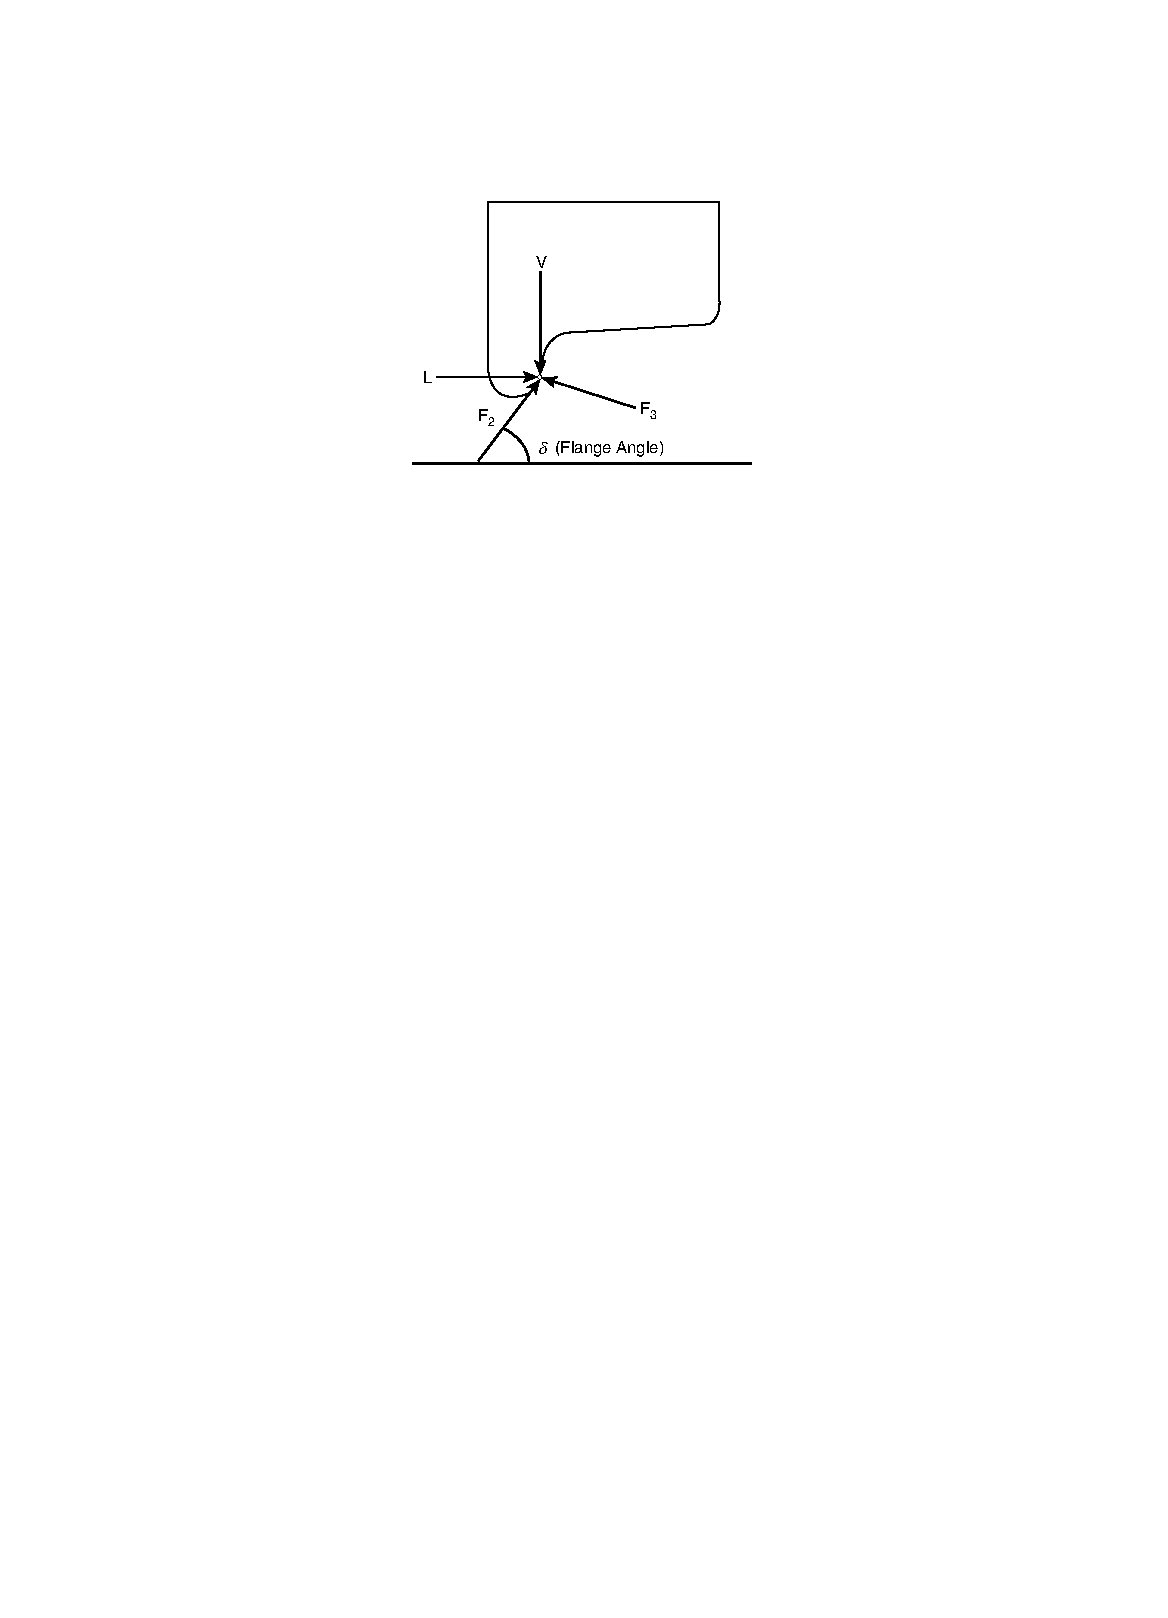
\includegraphics[width=0.4\textwidth]{forcesatflangecontactlocation.pdf}
	\caption{Forces at flange contact location. Extracted from \cite[Figure8.4]{iwnicki2006handbook}}
	\label{fig:forcesatflangecontactlocation}
\end{figure}

The criterion L/V ratio can be expressed as:

\begin{equation}
	\frac{L}{V}=\frac{\tan \delta -\frac{F_2}{F_3}}{1+\frac{F_2}{F_3}\tan \delta}
\end{equation}

Nadal's famous L/V ratio limiting criterion, given by Equation.\ref{eq:nadalcriterion}, was proposed for the saturated condition $F_2/F_3=\mu$

\begin{equation}\label{eq:nadalcriterion}
	\frac{L}{V}=\frac{\tan \delta - \mu}{1+ \mu \tan \delta}
\end{equation}

\subsubsection{Derailment caused by guage widening and rail rollover}
Derailments caused by guage widening usually involve a combination of wide gauges and large lateral rail defections(rail roll), as shown in Figure\ref{fig:gaugewideningderailment}. Large lateral forces from the wheels act to spread the rails in curves. Both rails may experience significant lateral translation and/or railhead roll, which often cause the nonflanging wheel to drop between rails.

\begin{figure}[h]
	\centering
	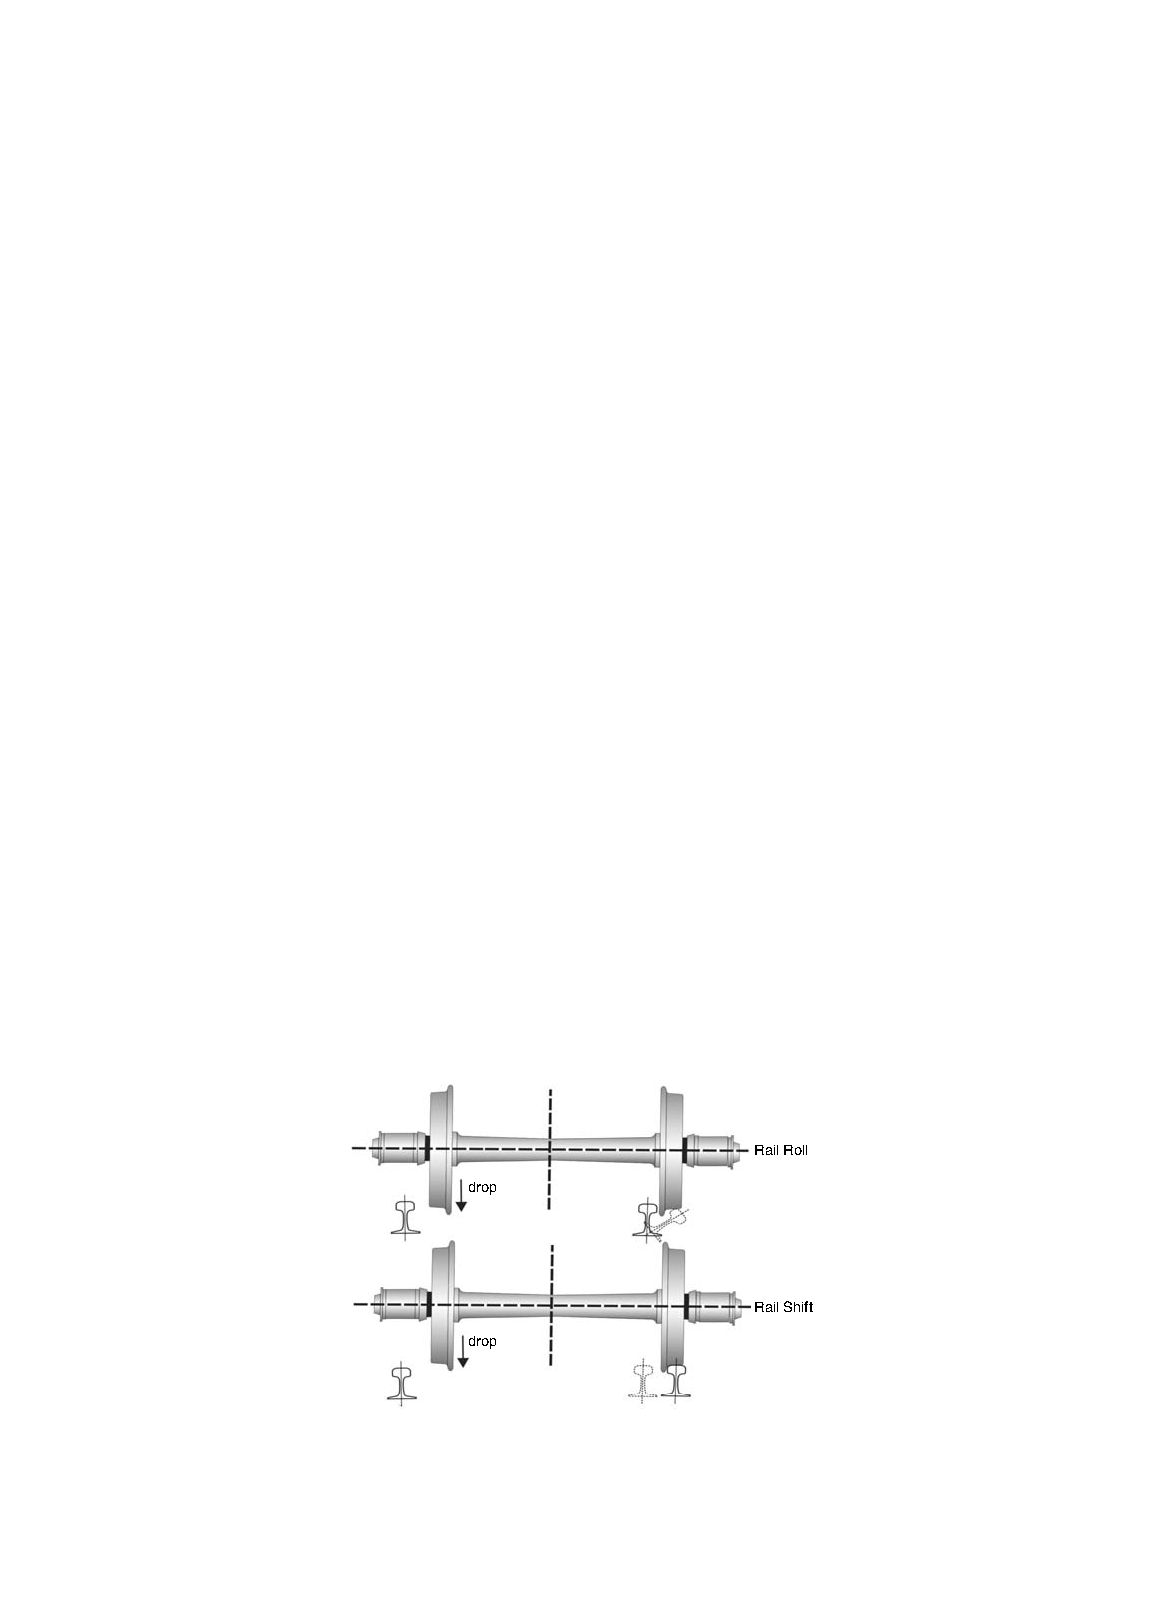
\includegraphics[width=0.8\textwidth]{gaugewideningderailment.pdf}
	\caption{Gauge widening derailment. Extracted from \cite[Figure8.18]{iwnicki2006handbook}}
	\label{fig:gaugewideningderailment}
\end{figure}

\paragraph{AAR Chapter XI rail roll criterion}
The AAR Chapter XI rail roll criterion is established by using the L/V ratio. The roll moment about the pivot point is given by,

\begin{equation}
	M=Vd-Lh
\end{equation}

under an equilibrium condition, just before the rail starts to roll, $M$ approaches to zero, then,

\begin{equation}
	\frac{L}{V}=\frac{d}{h}
\end{equation}

This L/V ratio is considered as the critical value to evaluate the risk of rail roll. When the L/V ratio is larger than the ratio of $d/h$, the risk of rail roll becomes high. The critical L/V ratio for rail roll can vary from above 0.6 for contact at the gauge side to approximately 0.2 when the contact position is at the far-field side based on the dimension of the rails. This is because the distance $d$ is reduced. Note that this L/V ratio is calculate assuming that neither the rail fasteners nor the torsional stiffness of the rail section provide any restraint.

\subsubsection{Derailment caused by track panel shift}
Track panel shift is the cumulative lateral displacement of the track panel, including rails, tie plates and ties, over the ballast, as shown in Figure\ref{fig:lateraltrackpanelshift}. A small shift of these components may not immediately cause the loss of guidance to bogies. However, as the situation gradually depreciates to a certain level, wheels could lose guidance and drop to the ground at some speed. The derailments caused by track panel usually result in one wheel falling between the rails and the other falling outside of the track.

\begin{figure}[h]
	\centering
	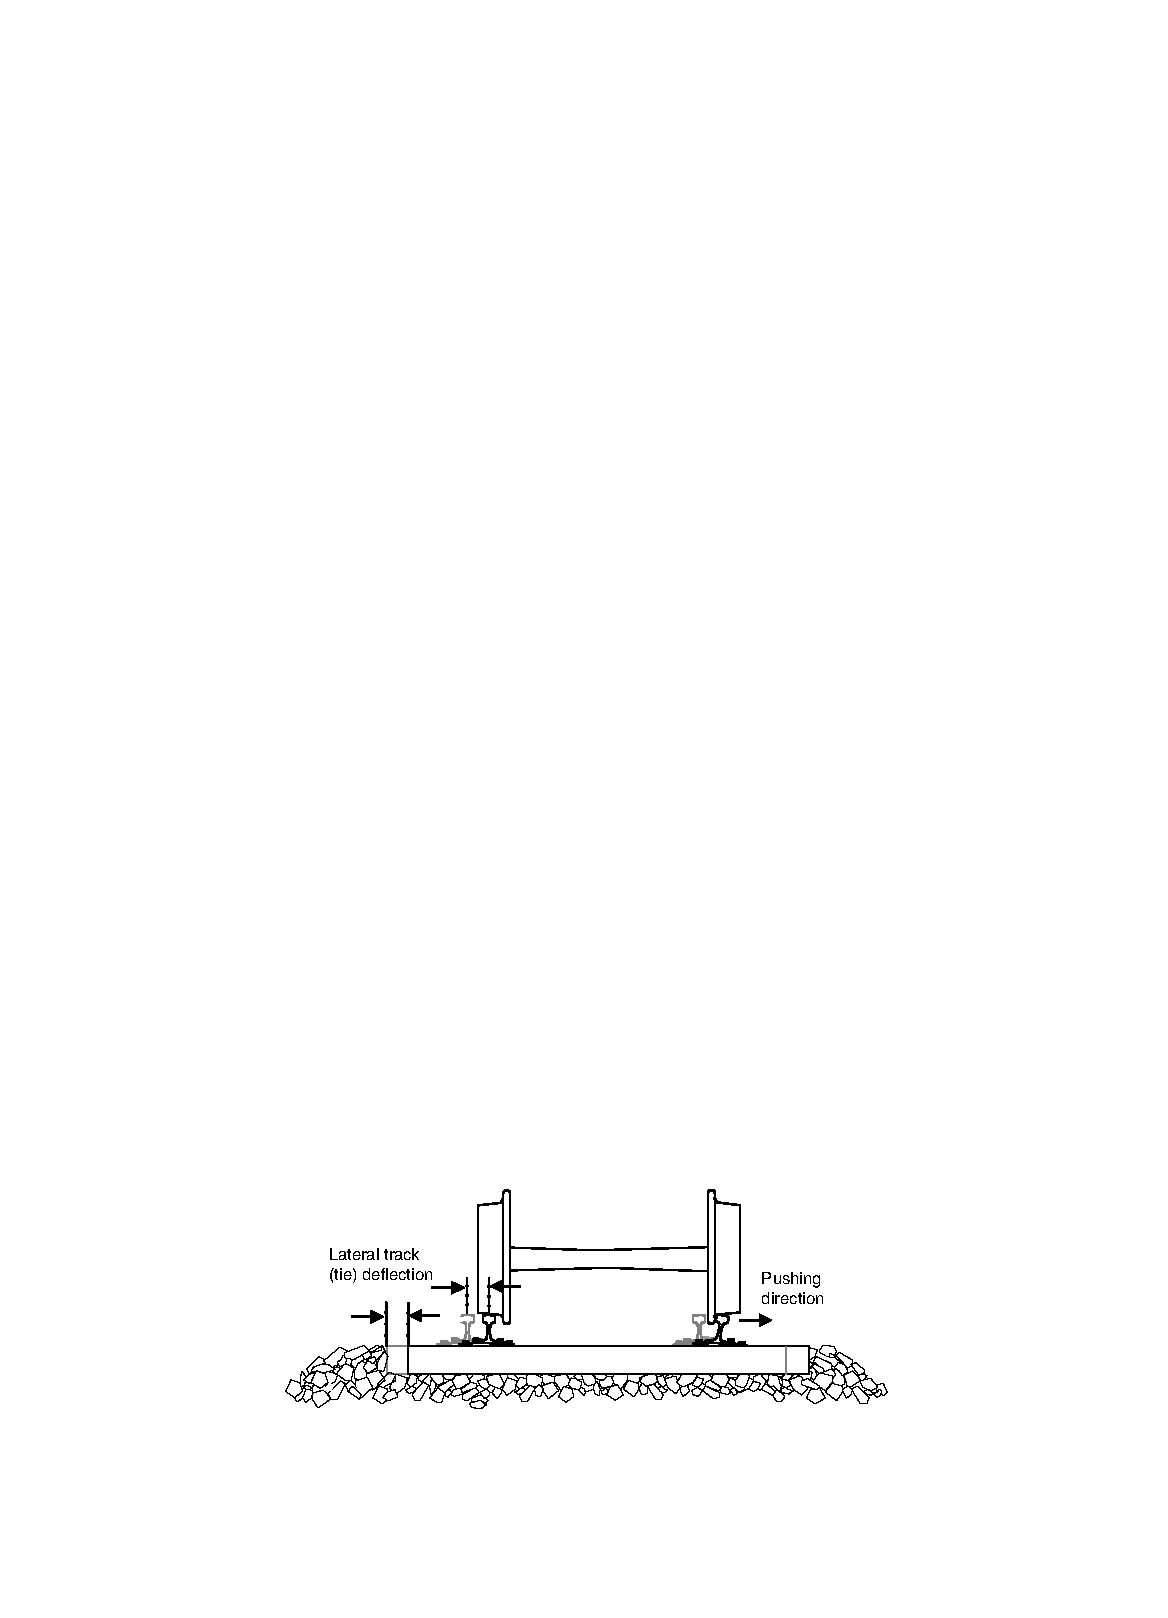
\includegraphics[width=0.8\textwidth]{lateraltrackpanelshift.pdf}
	\caption{Lateral track panel shift. Extracted from \cite[Figure8.27]{iwnicki2006handbook}}
	\label{fig:lateraltrackpanelshift}
\end{figure}

\paragraph{Panel shift criterion}
Researched by the French National Railways suggested that the limiting lateral axle load can be defined in a general expression for preventing excessive track panel shift:

\begin{equation}
	L_c = aV+b
\end{equation}

where $L_c$ is the critical lateral load and $V$ is the vertical axle load. \cite[Table 8.2]{iwnicki2006handbook} lists two groups of suggested valued of $a$ and $b$. It is possible that different values for $a$ and $b$ can be specified in different area.

\subsubsection{Derailment caused by vehicle lateral instability}
On tangent track, the wheelset generally oscillates around the track centre due to any vehicle and track irregularities, as shown in Figure\ref{fig:wheelsetoscillatesaroundthetrackcentre}. This movement occurs because vehicle and track are never absolutely smooth and symmetric. This self-centring capability of a wheelset is induced by the coned shape of the wheel tread. However, as speed is increased, if the whelset conicity is high, the lateral movement of wheelset, as well as the associated bogie and car body motion, can cause oscillations with large amplitude  and a well-defined wavelength. The lateral movements are limited only by the contact of the wheel flanges with the rail. This vehicle dynamic response is also termed as vehicle hunting, and can produce high lateral forces to damage track to cause derailments.

\begin{figure}[h]
	\centering
	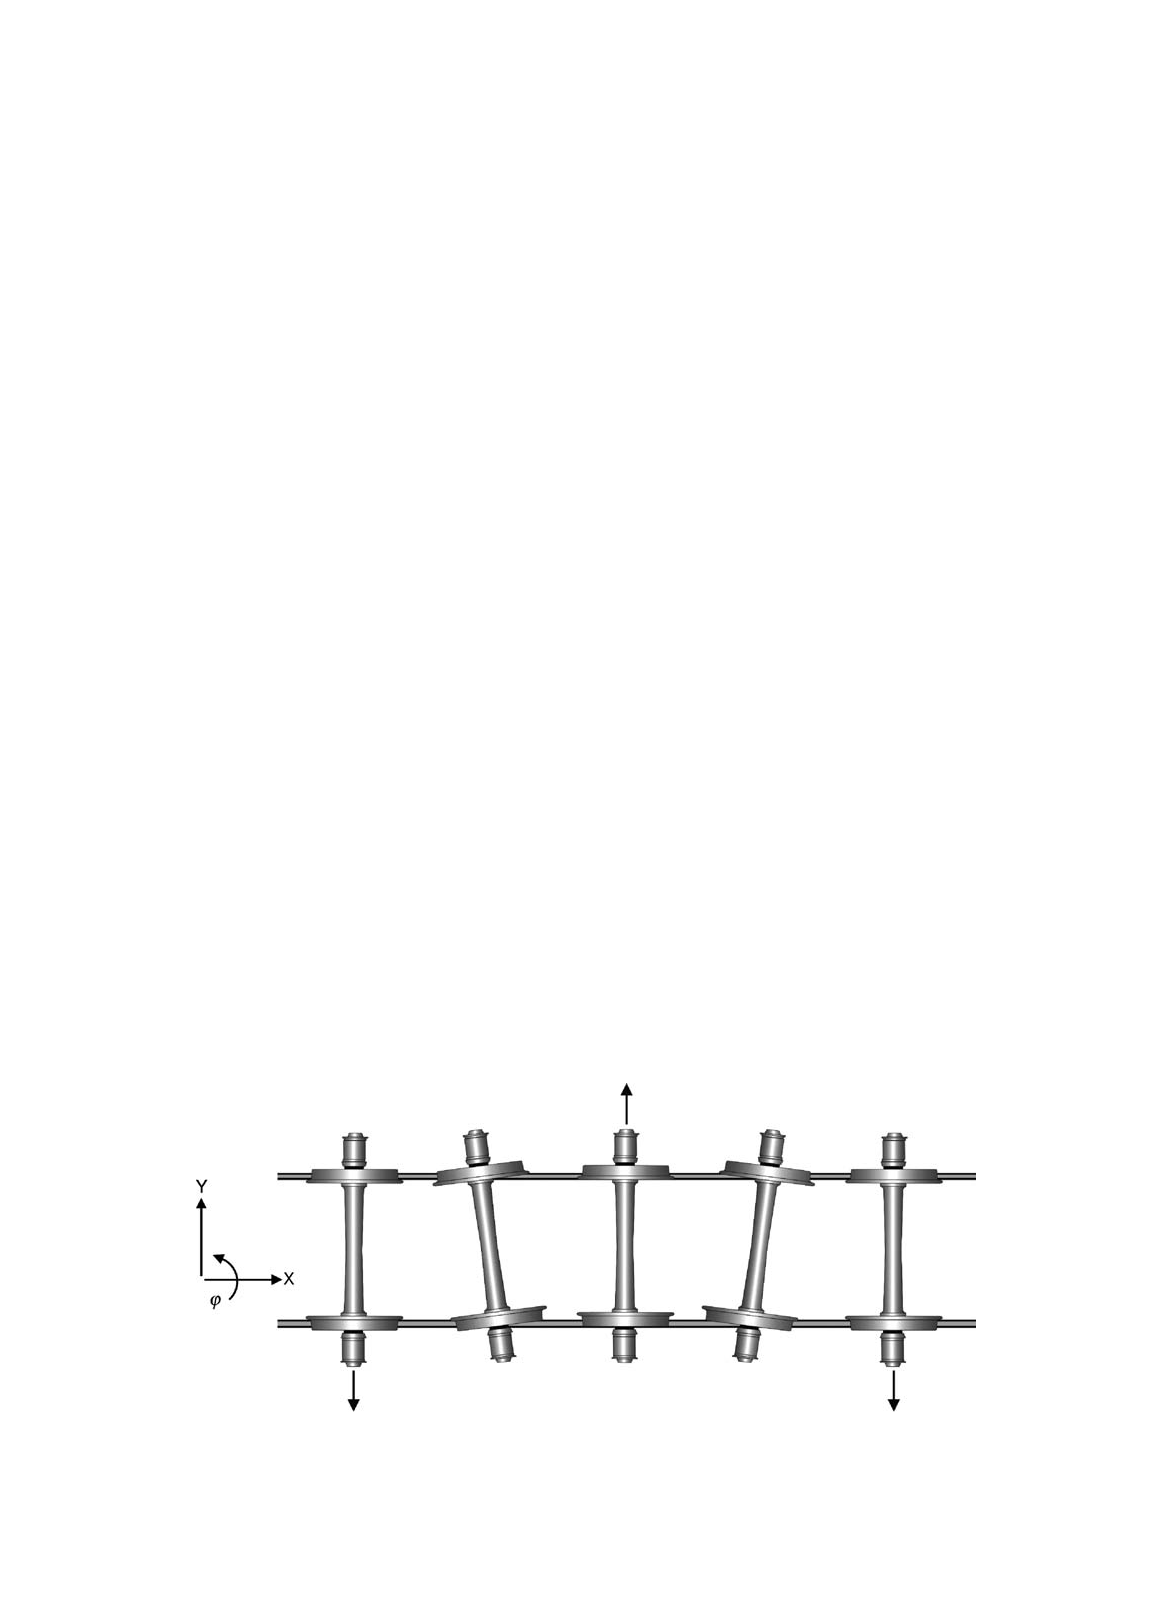
\includegraphics[width=0.8\textwidth]{wheelsetoscillatesaroundthetrackcentre.pdf}
	\caption{Wheelset oscillates around the track centre. Extracted from \cite[Figure8.28]{iwnicki2006handbook}}
	\label{fig:wheelsetoscillatesaroundthetrackcentre}
\end{figure}

Derailment cause by vehicle hunting can have derailment mechanisms of all four types discussed in the previous sections. The high lateral force induced from hunting may cause wheel flange climbing on the rail, gauge widening, rail roll-over, track panel shift, or combinations of these. The safety concerns for this type of derailment, usually occurring at higher speeds, make it an important area of study.

Hunting predominantly occurs in empty or lightweight vehicles. The critical hunting speed is highly dependent on the vehicle/track characteristics. Investigation of the critical speed for such a system with nonlinearities is to examine the vehicle response to a disturbance using a numerical solution of the equations of motion.

\subsection{Requirements for traffic serviceability(horizontal)}

The criteria Comfort Indexes for assessing ride comfort in railway vehicles proposed in \cite{12299}. This standard describes a methodology for assessing ride comfort as a function of longitudinal, vertical and transverse accelerations.

Comfort Index indicates the percentage of passengers experimenting discomfort in a specific situation. These indexes can be computed via empiric formula given in the standard, which depend on variables such as lateral acceleration, rate of change of acceleration and rolling velocity. All these values are filtered with a moving average filter that eliminates small wavelength components. Using this methodology for the computed worst-case situations, the comfort indexes have been found excellent, therefore no passenger should feel uncomfortable. 

\section{Torsional vibration}
According to \cite[9.1.3]{fryba1996dynamics}, the horizontal lateral forces of railway vehicles act on the rial top level,i.e. outside the cross section centroid of the bridge in the majority of cases. Let the difference of elevations be $ h $. Consequently, they affect the bridge by twisting moments $ hH_n(t) $. The differential equation of a beam due to simple torsion is 
\begin{equation}
	-GI_\xi \xi''(x,t)+\mu \ddot{\xi}(x,t)=\sum_{n=1}^{N}\varepsilon_n \delta (x+d_n-ct)h H_n(t)
\end{equation}

where $ \xi (x,t) $ is the rotation about the longitudinal beam axis x, $ G $ is the modulus of elasticity in shear, $ GI_\xi $ is the moment of torsional rigidity per unit length, $ \mu_\xi $ is the mass polar moment of inertia with regard to axis $ x $ per unit length.

\section{Theoretical bridge models}
According to \cite[Chapter.2]{fryba1996dynamics}, theoretical models of railway bridges are of two types

\begin{enumerate}[-]
	\item with continuously distributed mass
	\item with mass concentrated in material points(lumped mass)
	\item their combinations
\end{enumerate}

\subsection{Mass beams}
The most common simplified model for bridge is a simply supported Euler-Bernoulli beam model(see Figure.\ref{fig:massbeammodel}). The equation of motion of the beam expresses the equilibrium of forces per unit length:

\begin{figure}[h]
	\centering
	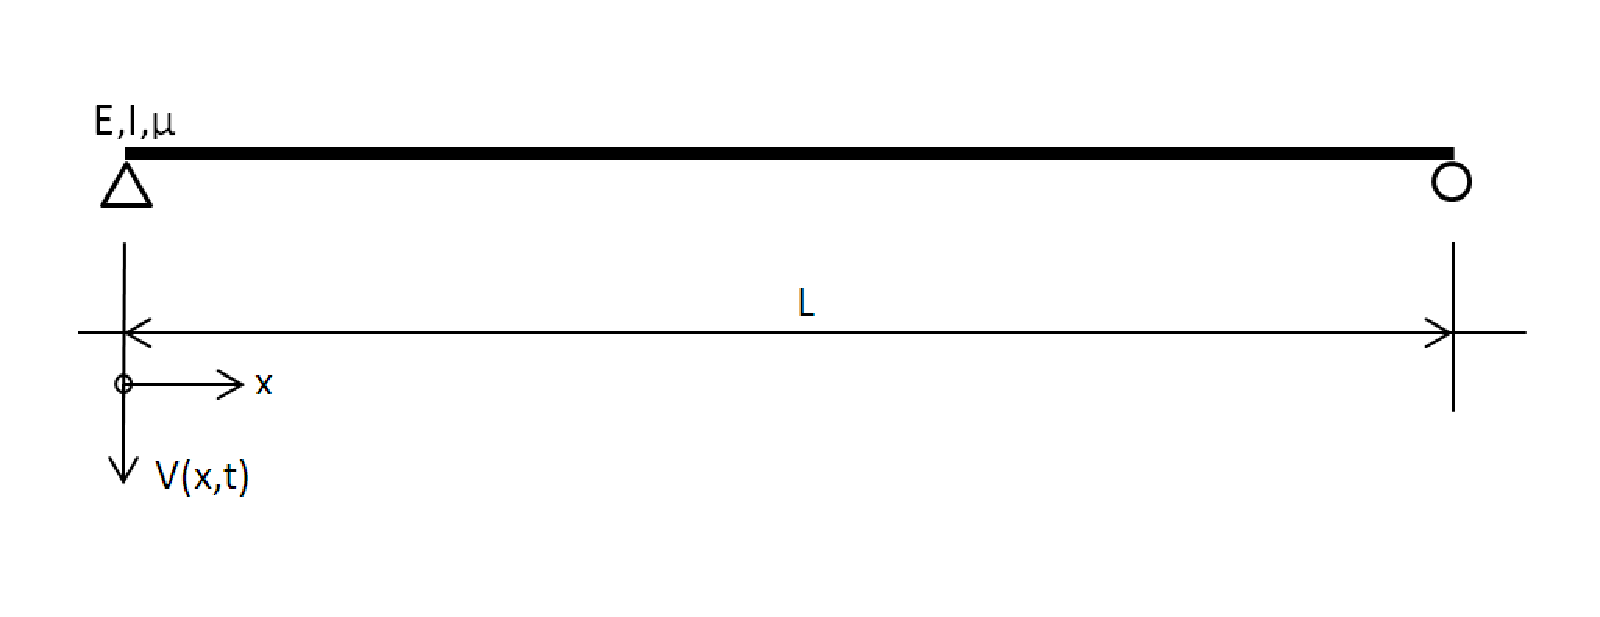
\includegraphics[width=0.8\textwidth]{massbeammodel.pdf}
	\caption{Mass beam model of span L}
	\label{fig:massbeammodel}
\end{figure}

\begin{equation}
	EI\dfrac{\partial^4v(x,t)}{\partial x^4}+\mu \dfrac{\partial^2 v(x,t)}{\partial t^2} + 2\mu \omega_b \dfrac{\partial v(x,t)}{\partial t} = f(x,t)
	\label{eq:massbeammodel}
\end{equation}

where:
\begin{enumerate}[]
	\item $ v(x,t) $:vertical deflection of the beam at the point $ x $ and at time $ t $
	\item $ E $:modulus of elasticity of the beam
	\item $ I $:moment of inertia of beam cross section
	\item $ \mu $:mass per unit length of the beam
	\item $ \omega_b $:circular frequency of viscous damping
	\item $ f(x,t) $:load at point $ x $ and time $ t $ per unit length of the beam
\end{enumerate}

\subsection{Continuous beam}
The continuous beam model is suitable for multi-span bridges in general. The equation of motion is the same as simple beam model in Equation\ref{eq:massbeammodel}. 

\begin{figure}[h]
	\centering
	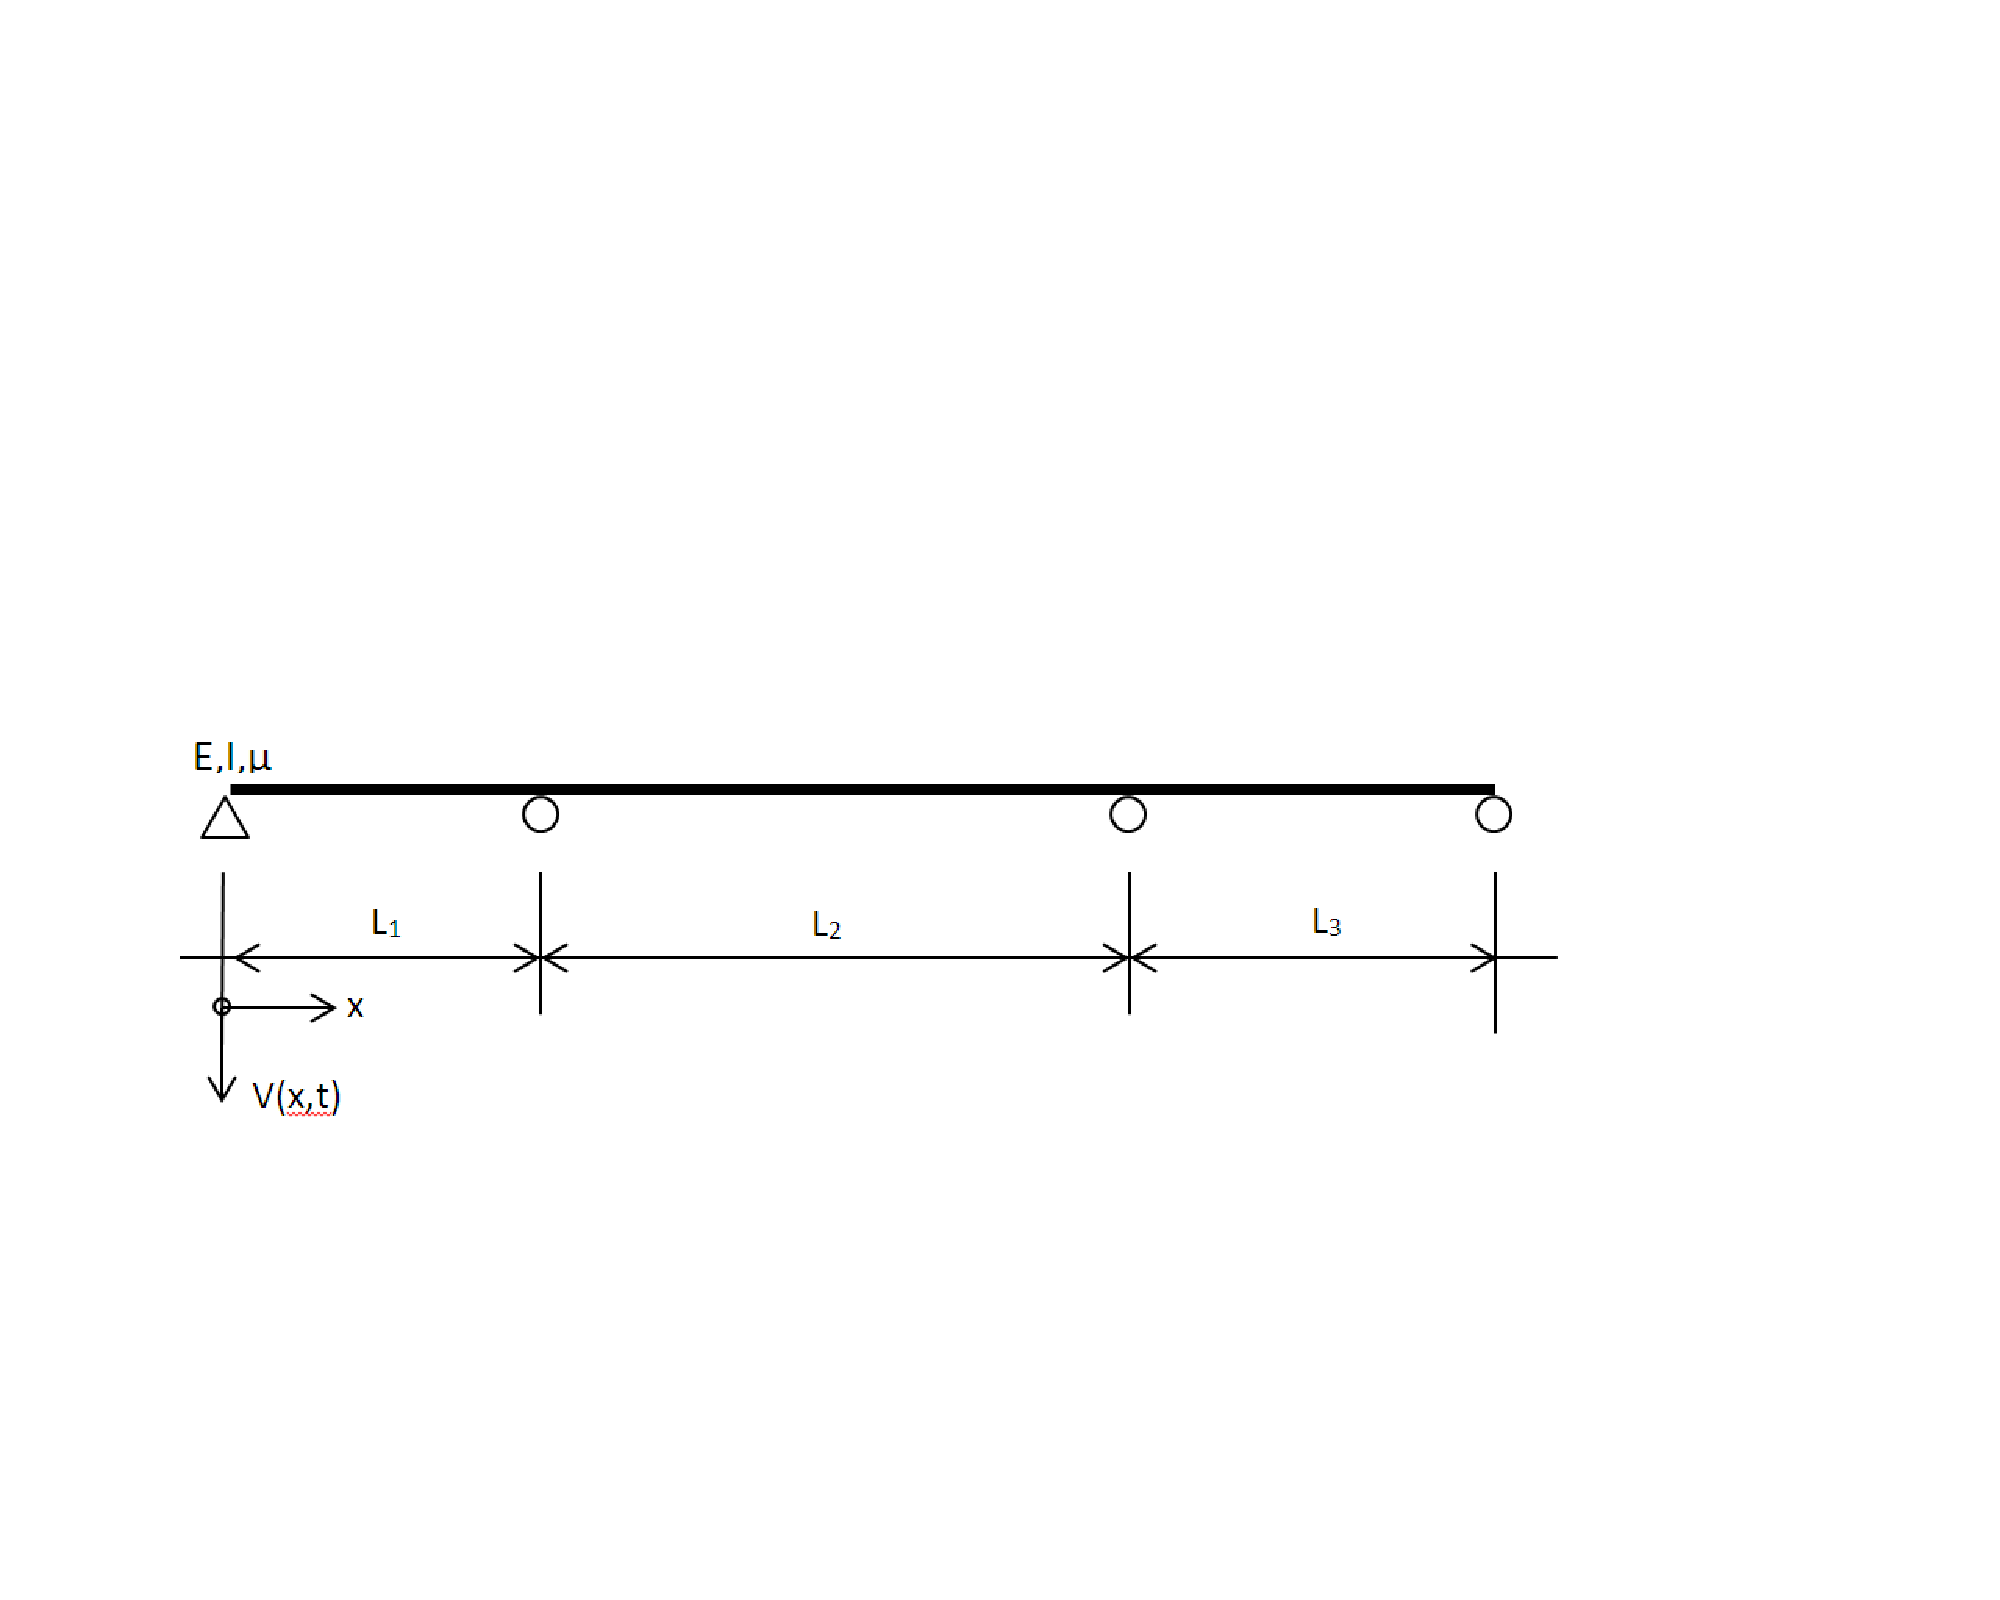
\includegraphics[width=0.8\textwidth]{continuousbeammodel.pdf}
	\caption{Continuous beam model}
	\label{fig:continuousbeammodel}
\end{figure}
	
\subsection{Complex systems}

\subsubsection{Trusses}

\subsubsection{Frames}

\subsubsection{Curved bars}

\subsection{High strength steel bridges}
The advantage of high strength steel bridges are

\begin{enumerate}
	\item High quality material
	\item Speed of construction
	\item Versatility
	\item Modification and repair
	\item Recycling
	\item Durability
	\item Aesthetics
\end{enumerate}

\cite{macdougall2004state}: Use of high-strength steels for bridge construction in Japan dates back to the 1960s. Several hundred bridges been constructed using 500MPa and 600MPa yield strength steel, and steel with a normal yield strength of 800 MPa has also been used on several projects. In Europe, a variety of high-strength steels with yield strength from 460MPa to 690MPa are available for bridge applications. European structural steel standard EN 10025: 2004 grade S460ML, which has a nominal yield strength of 460MPa, can be welded at room temperature for plate thickness up to 90mm and has a specified minimum Charpy V-notch(CVN) evergy of 27 J at -50$^\circ$C.

\section{Modelling of railway vehicles}
According to Newton's law, 2 basic load effects are produced by moving train: vertical forces due to vehicle weight, and inertia effects caused by vehicle acceleration. The loads on a railway bridge are very complex problems thus in engineering practice, loads are often simplified. But, the simplification depends on the purpose of the analysis. 

\subsection{Moving vertical forces model}
If the inertia effects are neglected, loads of the moving trains can be modelled as moving vertical forces. For example, load diagram for type TALGO trains is shown in Figure.\ref{fig:verticalmodel} proposed by \cite{uic}.

\begin{figure}[h]
	\centering
	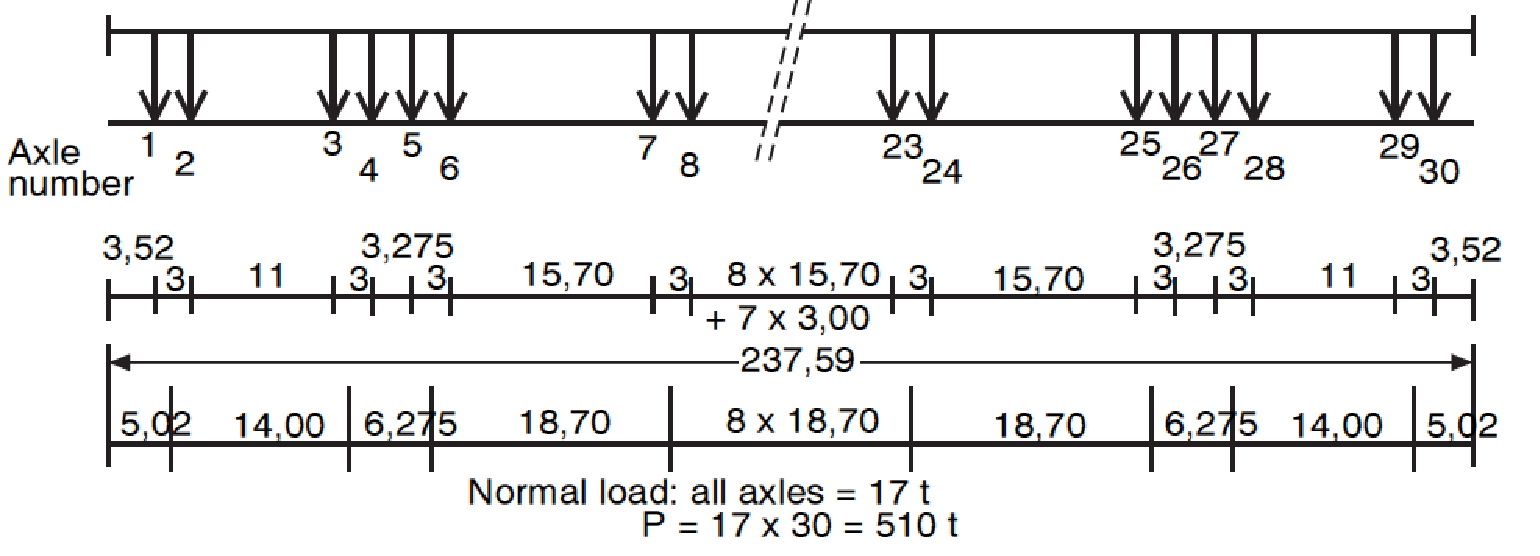
\includegraphics[width=0.8\textwidth]{verticalmodel.pdf}
	\caption{Moving vertical force model for TALGO trains}
	\label{fig:verticalmodel}
\end{figure}

\subsection{Advanced models}
Nowadays more and more models have been proposed to meet different requirements of railway bridge dynamic analysis. The complexity of these models differs from each other but they are all more complicated than moving vertical forces models. For example, vehicle-bridge interaction model takes vehicle suspension system into account, which gives an alternative for discovering resonance effects between bridge and the vehicle suspension systems. 

See Figure.\ref{fig:advancedmodel} for an example of advanced model.

\begin{figure}[p]
	\centering
	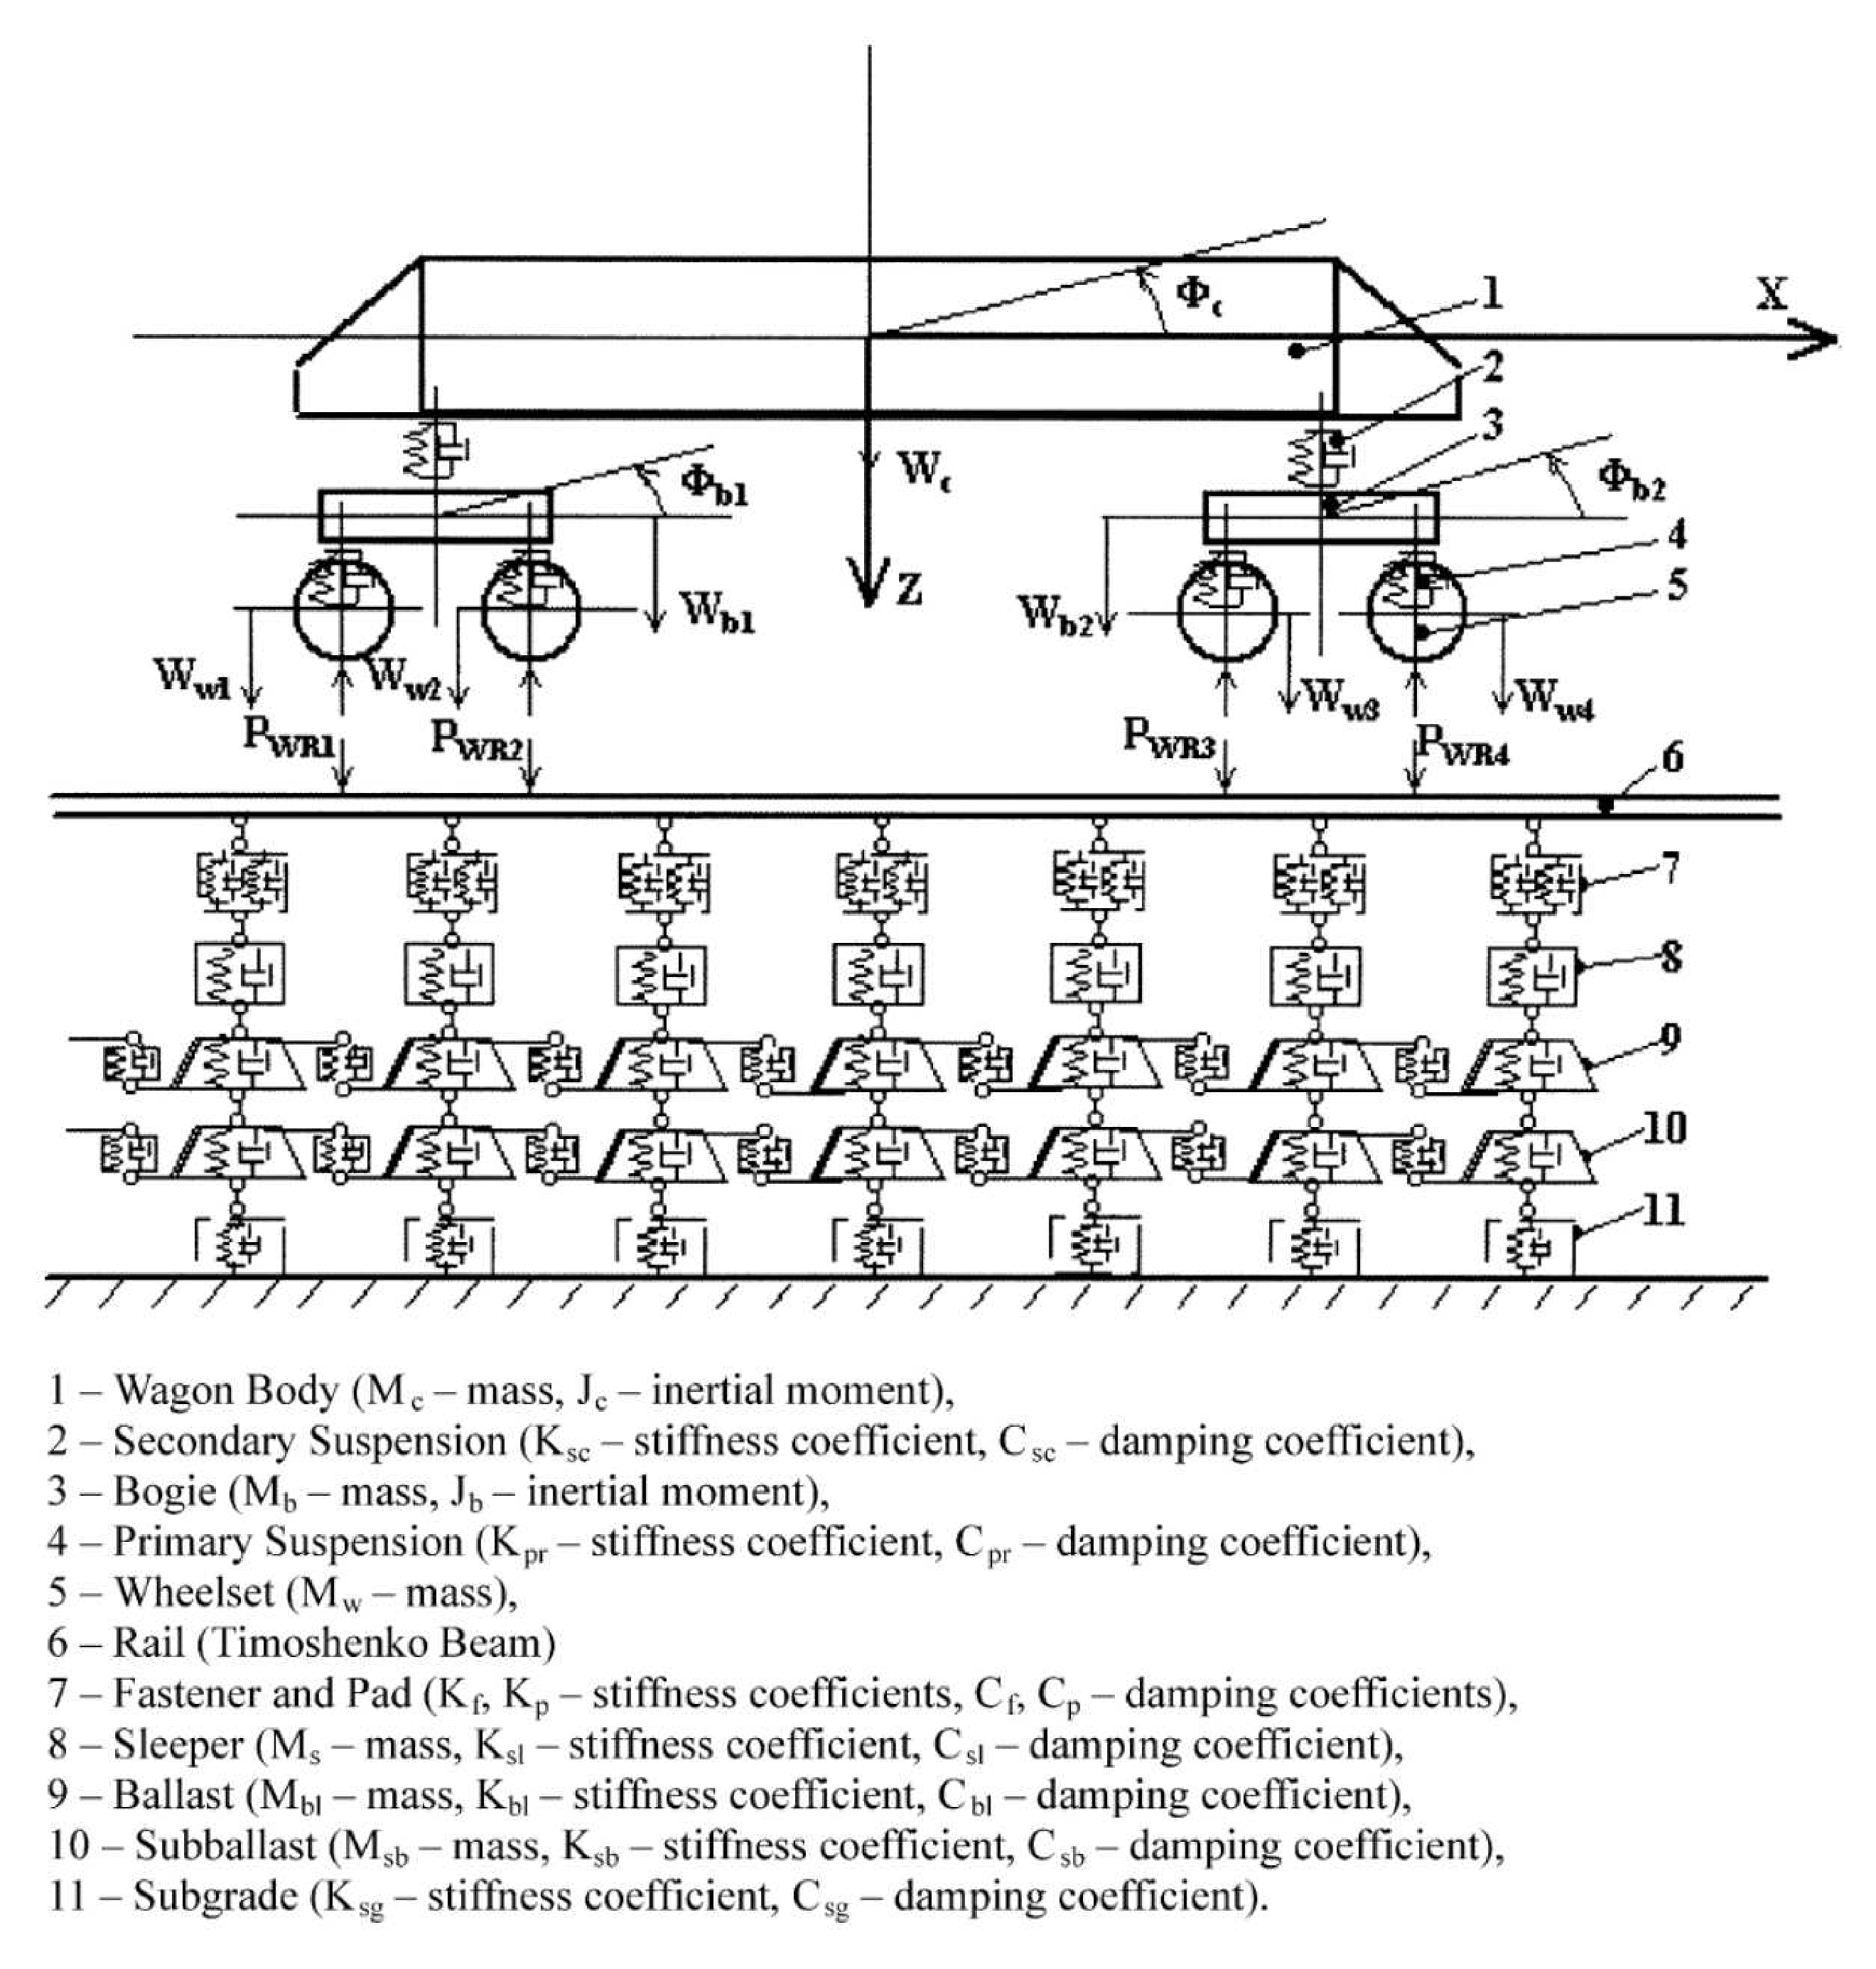
\includegraphics[width=0.8\textwidth]{advancedmodel.pdf}
	\caption{A dynamic model for the vertical interaction of the rail track and wagon system. Proposed in \cite{sun2002dynamic}}
	\label{fig:advancedmodel}
\end{figure}


\subsection{Models proposed in Eurocodes}

See Chapter~\ref{sec:train-models}

\section{Track model}
Proposed in \cite[A.6.1.3]{uic}, the track is represented by Timoshenko beam elements for the rails and takes account of the rail/sleeper fastening characteristics as well as the ballast(if one exists).

\textit{``A sleeper is generally represented by two beam elements, with two covering the rail and one used for the deck. Sleepers and ballast are modelled as concentrated masses. They are linked to the nodes of the rail and the bridge by a parallel spring and damper system. The track can be modelled to any length on both side of the bridges, where the stiffening effect of the bridge has to be taken into account. The effects of track distribution are not considered. Each vehicle is able to absorb the kinetic energy of the bridge and it is for this reason that, at resonance, the deflections and accelerations of the bridge obtained with this model are lower than those obtained with a live load diagram."}

The most complete model for analysing train/track/bridge interaction is shown in Figure

\begin{figure}[h]
	\centering
	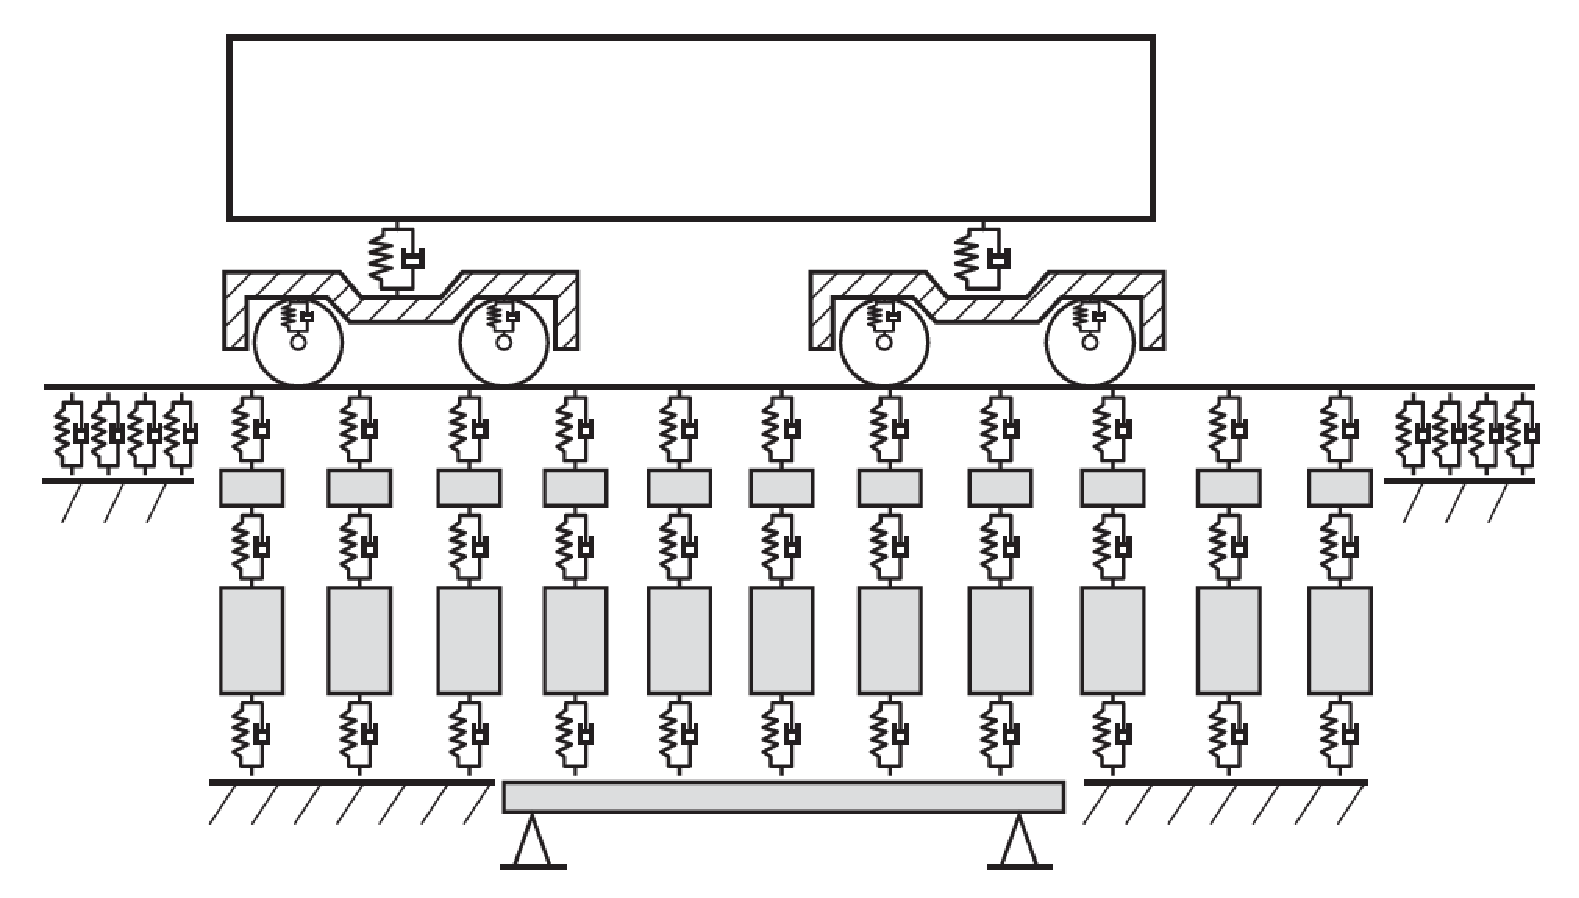
\includegraphics[width=0.8\textwidth]{trackmodel.pdf}
	\caption{Diagram of the dynamic train-track-bridge model. Extracted from \cite[Fig. 15]{uic}}
	\label{fig:trackmodel}
\end{figure}


\section{General design principles and procedures concerning railway bridge dynamics proposed by Eurocodes } \label{designprocedures}


\subsection{Requirements for railway bridge verification}
\cite{EC0} propose following requirements


\begin{enumerate}
	\item Checks on bridge deformations shall be performed for traffic safety purposes for the following items:
	\begin{enumerate}[-]
		\item vertical accelerations of the deck
		\item vertical deflection of the deck throughout each span
		\item unrestrained uplift at the bearings(to avoid premature bearing failure)
		\item vertical deflection of the end of the deck beyond bearings(to avoid destabilising the track, limit uplift forces on rail fastening systems and limit additional rail stresses) 
		\item twist of the deck measured along the centre line of each track on the approaches to a bridge and across a bridge(to minimise the risk of train derailment)
		\item rotation of the ends of each deck about a transverse axis or the relative total rotation between adjacent deck ends(to limit additional rail stresses, limit uplift forces on rail fastening systems and limit angular discontinuity at expansion devices and switch blades)
		\item longitudinal displacement of the end of the upper surface of the deck due to longitudinal displacement and rotation of the deck end(to limit additional rail stresses and minimise disturbance to track ballast and adjacent track formation)
		\item horizontal transverse deflection(to ensure acceptable horizontal track radii)
		\item horizontal rotation of a deck about a vertical axis at ends of a deck (to ensure acceptable horizontal track geometry and passenger comfort)
		\item limits on the first natural frequency of lateral vibration of the span to avoid the occurrence of resonance between the lateral motion of vehicles on their suspension and the bridge
	\end{enumerate}
	\item Checks on bridge deformations should be performed for passenger comfort, i.e. vertical deflection of the deck to limit coach body acceleration in accordance with A2.4.4.3\cite{EC0}
	\item The limits given in A2.4.4.2 and A2.4.4.3\cite{EC0} take into account the mitigating effects of track maintenance (for example to overcome the effects of the settlement of foundations, creep, etc.) 
\end{enumerate}

\subsection{Conceptual check}
The conceptual check is to help designers avoid unsafe designs in conceptual stage. Once the bridge type and rough geometry is sketched, designers can easily know whether the bridge would have dynamic problem in the future. 

For example, in  \cite[cl.8.7.4]{calgaro2010designers}, it is stated that if the bridge meets criteria ~\ref{cr:nocheck} , no dynamic analysis in necessary. 

\begin{equation}
	\label{cr:nocheck}
	V>200km/h \quad \delta_{dyn} \leq \text{ value given by the dynamic study, but }\delta_{stat}\leq L/2600
\end{equation}

On the other hand, no other conceptual check criterion is given for train speed under 200km/h. Since there is higher possibility that, for bridges with span larger than 100m, they will have resonance with the normal trains. 

\subsection{Logic diagram}

This logic diagram is used to determine whether a dynamic analysis is required, as shown in Figure~\ref{fig:logicdiagram}, is represented in \cite{EC12} Chapter 6.4 Dynamic Effects, where $V [Km/h]$ is the Maximum Line Speed at the site, $L [m]$, the span length, $n_0 [Hz]$, the first nature frequency under permanent loads, $n_T$, the first natural torsional frequency for the same load, $v [m/s]$ the maximum nominal speed and finally $(v/n_0)_{lim}$, as given in Annex F of EN1991-2. The frequency first of vibration, $n_0$, must be within the limits established in figure~\ref{fig:frequencylimit}.

Checking through the logic diagram is regarded as first step is because designers can try to avoid designs that will be required to be dynamic analysed in the very beginning of the designing phase. 

The upper limit (1) is defined as

\begin{equation}
	n_0=94,76L^{-0,748}
\end{equation}

and the lower limit (2) as:

\begin{equation}
	n_0= \{ \begin{array}{ll}
	80/L & \mbox{for $4m\leq L \leq 20m$} \\
	94,76L^{-0,748} & \mbox{for $20m\leq L \leq 100m$}
\end{array} 
\end{equation}

\begin{figure}[h]
\centering
	\begin{subfigure}[b]{0.45\textwidth}
    	\centering
    	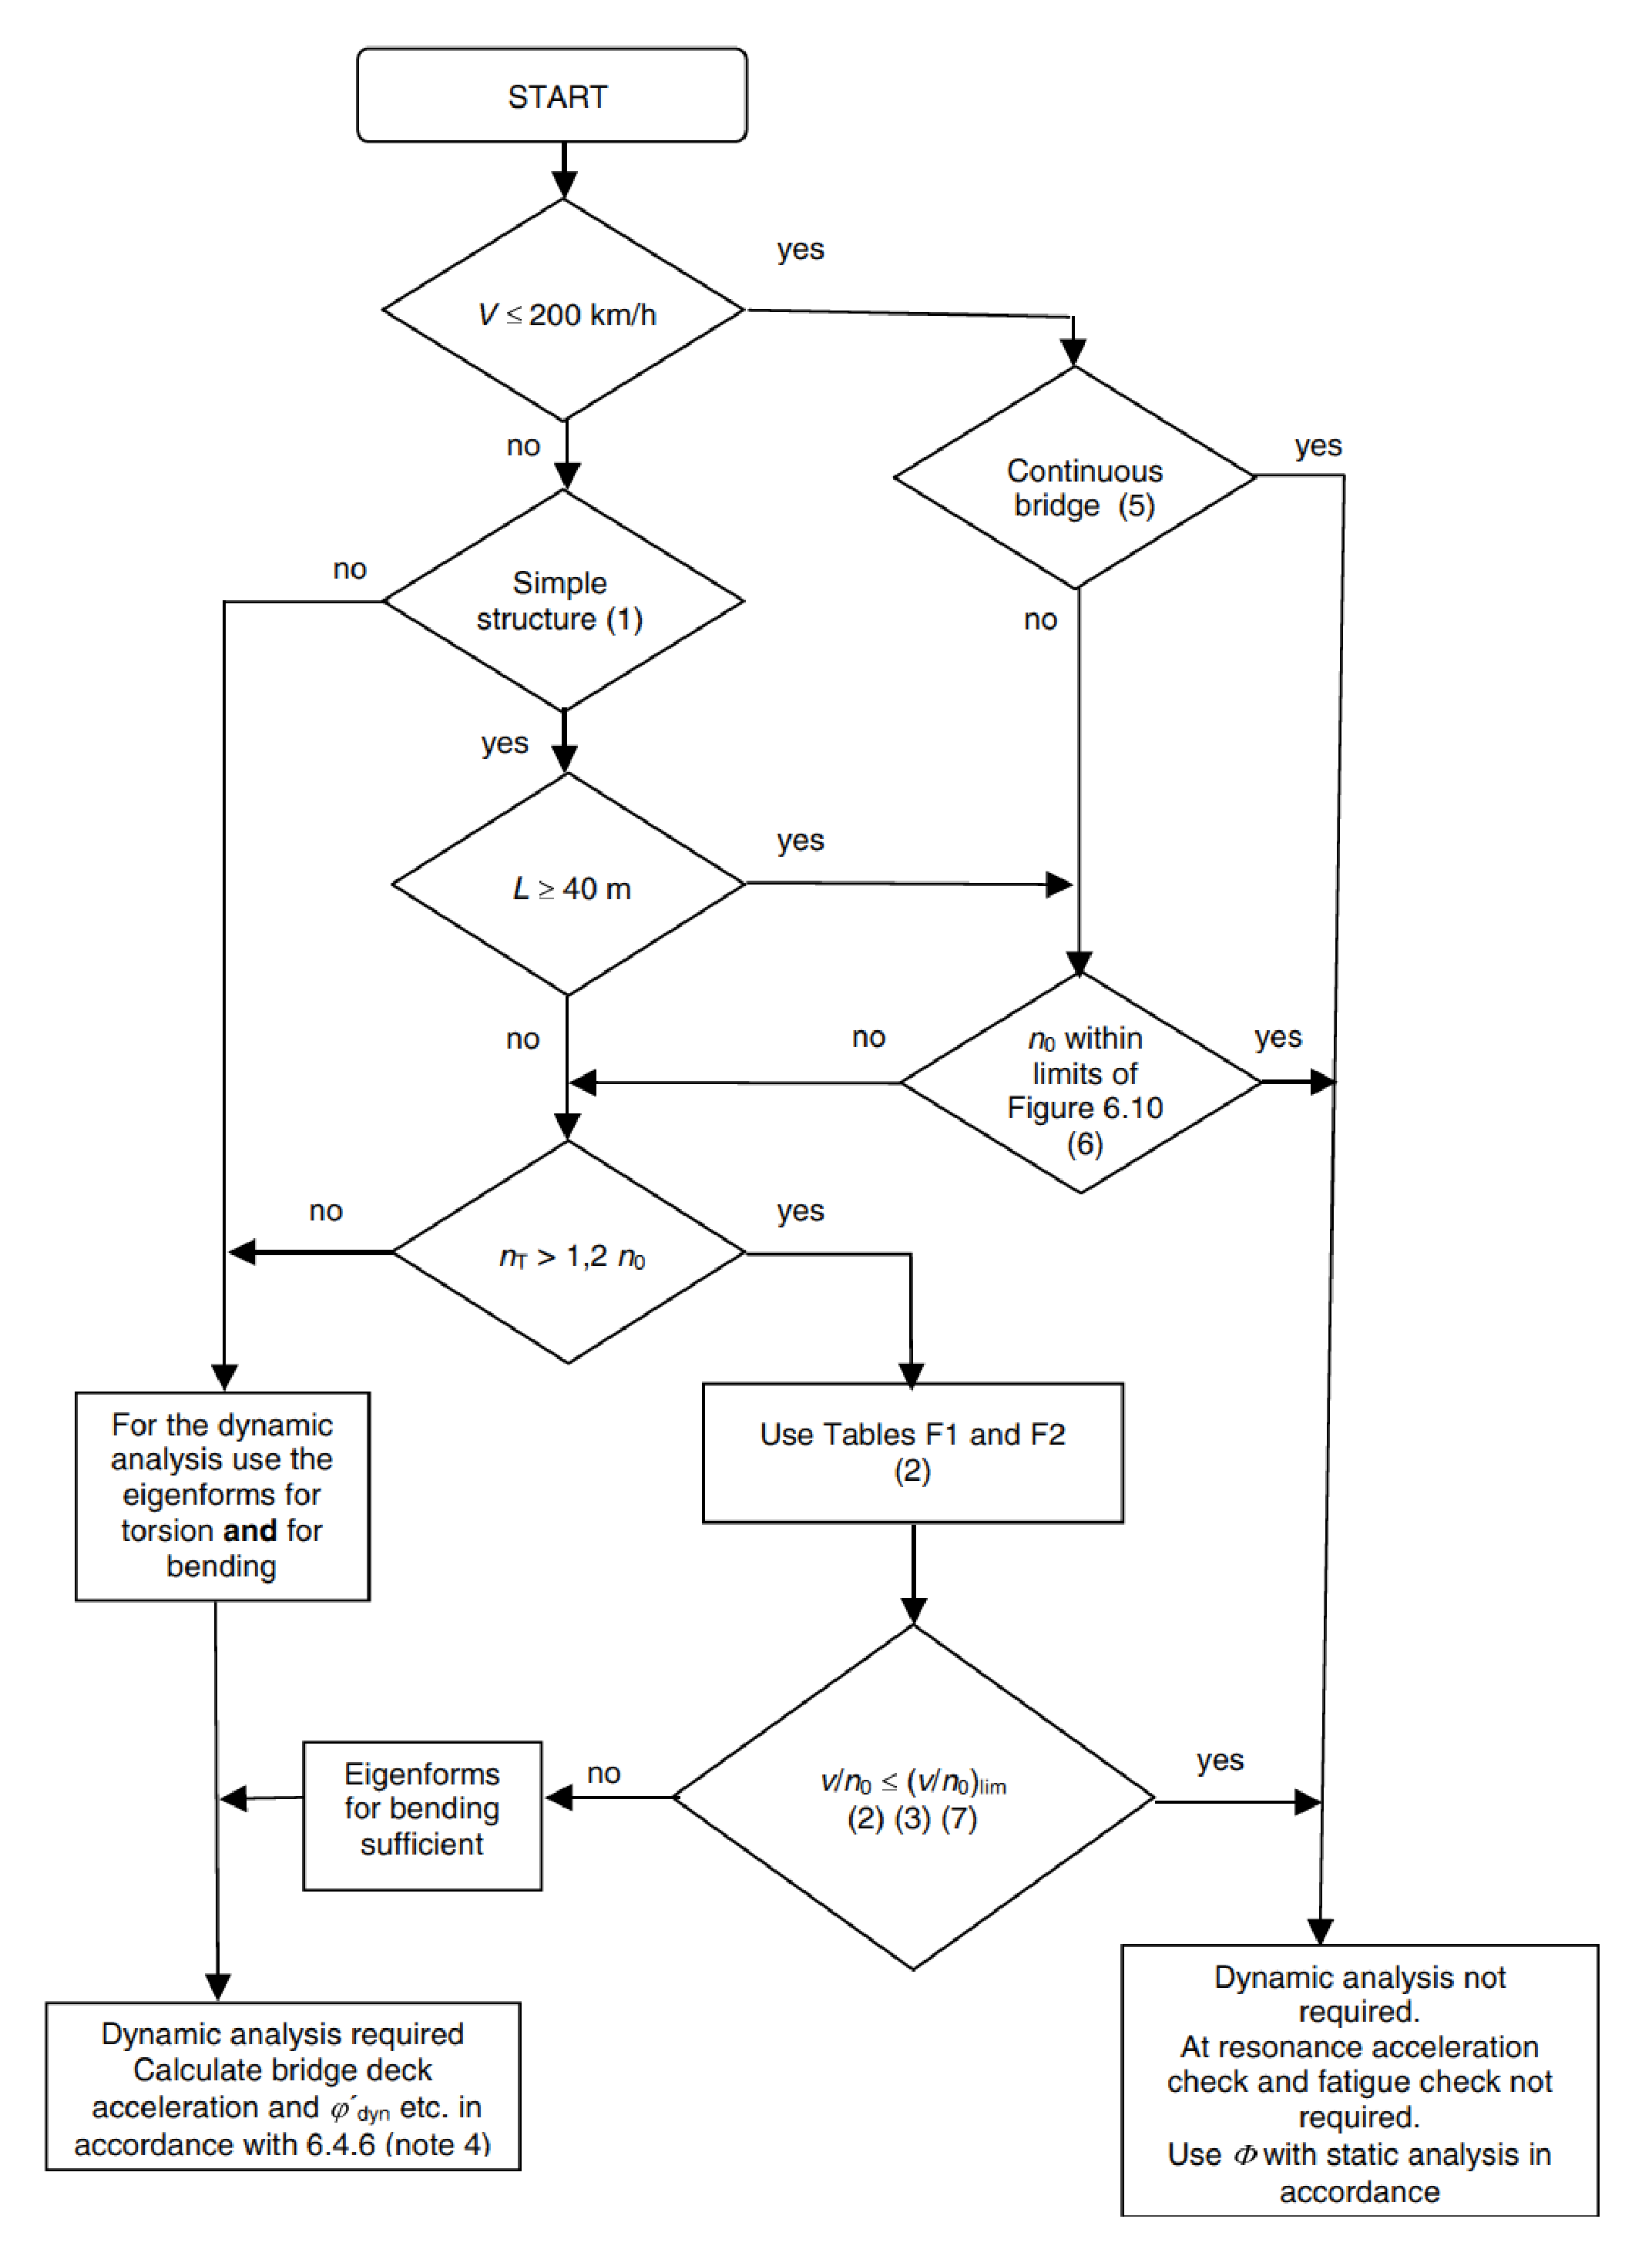
\includegraphics[width=\textwidth]{logicdiagram.pdf}
    	\caption{Flow chart for determining whether a dynamic analysis is required. Extracted from EN1991-2\cite{EC12}}
    	\label{fig:logicdiagram}
	\end{subfigure}
	\begin{subfigure}[b]{0.45\textwidth}
    	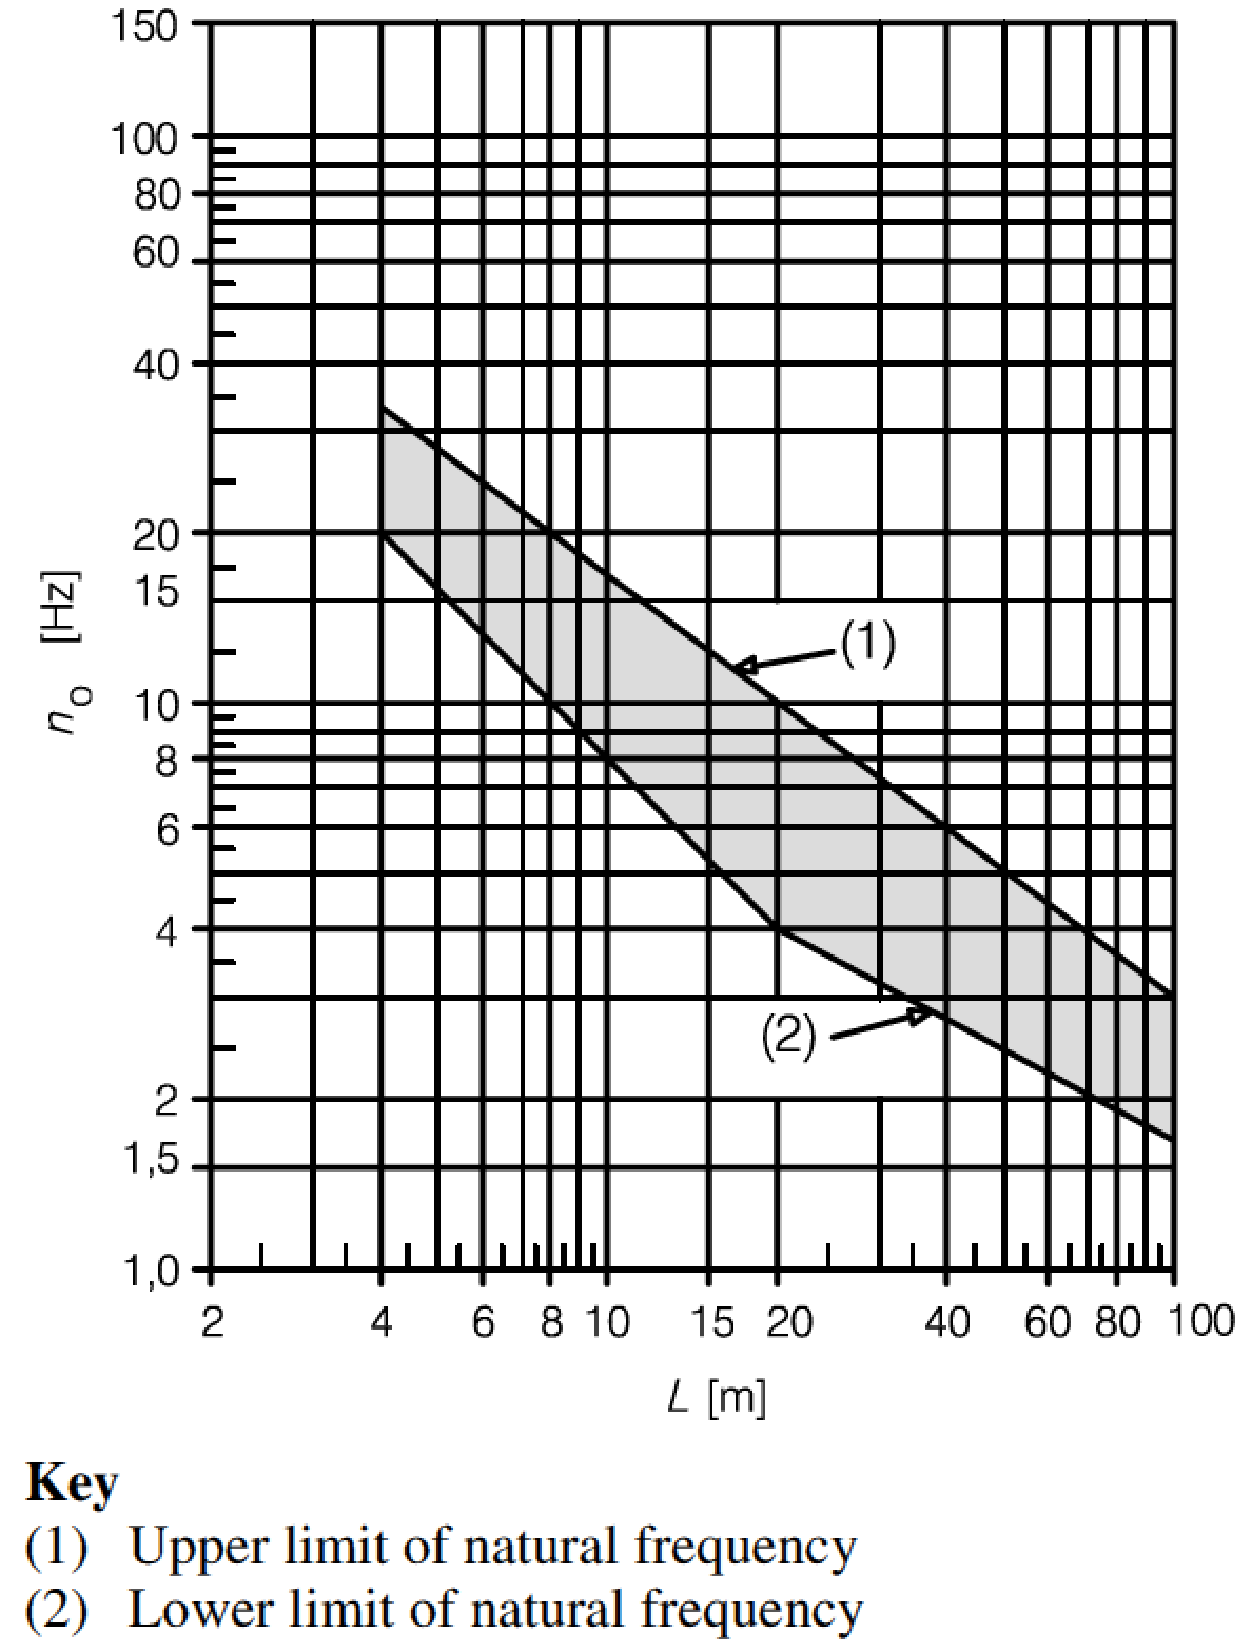
\includegraphics[width=\textwidth]{frequencylimit.pdf}
    	\caption{Limits for bridge natural frequencies, $n_0 [Hz]$, as a function $L [m]$. Extracted from EN1991-2\cite{EC12}.}
    	\label{fig:frequencylimit}
	\end{subfigure}
\caption{Logic diagram for determining whether dynamic analyses are necessary, extracted from \cite[6.4.4]{EC12}}
\label{logicandlimit}
\end{figure}

\subsection{Train models}\label{sec:train-models}
According to NEN 1991-2\cite{EC12} and Designers Guide\cite{calgaro2010designers} Rail traffic actions are defined by means of load models, Four models of railway loading are given:
\begin{enumerate}[$\bullet$]
	\item LM71 and LM SW/0(for continuous bridges) to represent normal rail traffic on mainline railways (passenger and heavy freight traffic)
	\item SW/2 to represent abnormal loads or waggons
	\item LM 'unloaded train' to represent the effect of an unloaded train
	\item LM HSLM (comprising HSLM-A and HSLM-B) to represent the loading from passenger trains at speeds exceeding 200km/h.
\end{enumerate}

\subsubsection{Load Model 71}
LM71 represents the static effect of vertical loading due to normal rail traffic.

The load arrangement and the characteristic values for vertical loads have to be taken as shown in Figure.~\ref{lm71}

The actions listed below, associated with LM71, have to be multiplied by factor $ \alpha $:

\begin{enumerate}[-]
	\item equivalent vertical loading for earthworks and earth pressure effects
	\item centrifugal forces
	\item nosing force (multiplied by $ \alpha $ for $ \alpha\geq 1 $ only)
	\item traction and braking forces
	\item derailment actions for accidental design situations
	\item Load Model SW/0 for continuous span bridges
\end{enumerate}

\textit{For international lines, it is recommended that a value of $ \alpha \geq 1.0 $ is adopted. But this freedom of choice of the factor $ \alpha $ could lead to a non-uniform railway network in Europe. Therefore in UIC Code 702\textsuperscript{4} $ \alpha=1.33 $ is generally recommended for all new bridges constructed for the international freight network, but not compulsory}. 

\begin{figure}[h]
	\centering
	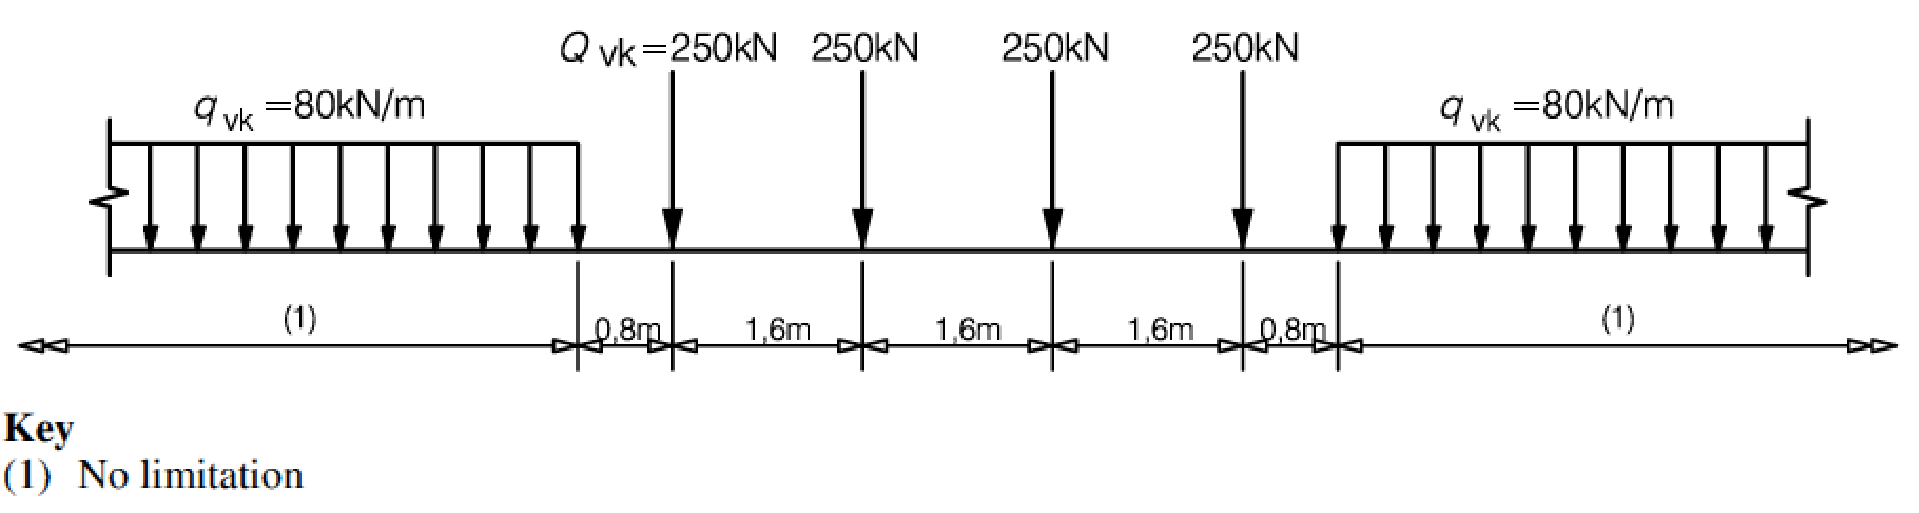
\includegraphics[width=0.8\textwidth]{lm71.pdf}
	\caption{Load Model 71 and characteristic values for vertical loads. Extracted from EN1991-2\cite{EC12}}
	\label{lm71}
\end{figure}

\subsubsection{Load Models SW/0 and SW/2}
Load Models SW/0 represents the static effect of vertical loading due to normal rail traffic on continuous beams.

Load Model SW/2 represents the static effect of vertical loading due to heavy abnormal rail traffic. 

The load arrangement is as shown in Figure.~\ref{lmsw}, with the characteristic values of the vertical loads according to Table.\ref{tab:sw}

\begin{figure}[h]
	\centering
	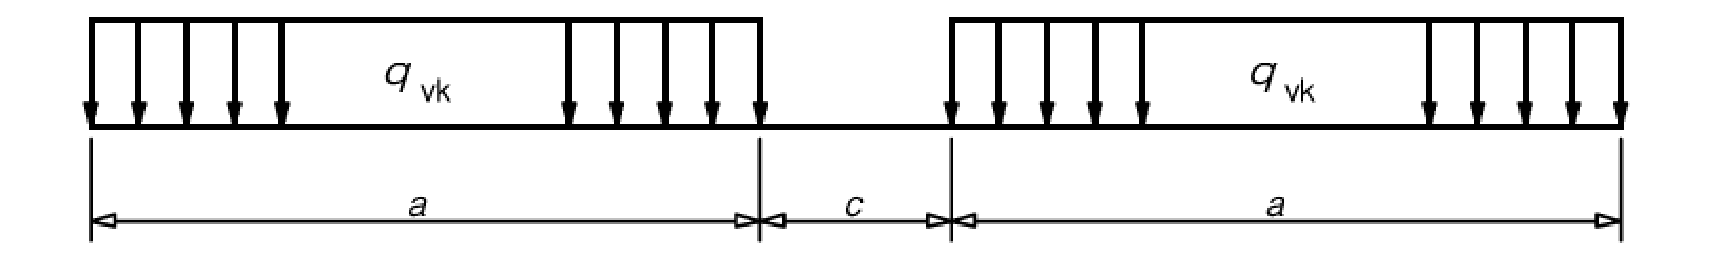
\includegraphics[width=0.8\textwidth]{lmsw.pdf}
	\caption{Load Models SW/0 and SW/2.. Extracted from EN1991-2\cite{EC12}}
	\label{lmsw}
\end{figure}

\begin{table}[h]
	\centering
	\begin{tabular}{llll}
		\hline
		Load model & $ q_{vk} (kN/m) $ & $ a (m) $ & $ c (m) $ \\
		\hline
		SW/0 & 133 & 15.0 & 5.3\\
		SW/2 & 150 & 25.0 & 7.0\\
		\hline
	\end{tabular}
	\caption{Characteristic values for vertical loads for Load Models SW/0 and SW/2}
	\label{tab:sw}
\end{table}

\subsubsection{Load Model 'unloaded train'}
From some specific verification purposes a specific load model is used, called 'unloaded train'. The Load Model 'unloaded train' consists of a vertical uniformly distributed load with a characteristic value of 10.0kN/m.

\subsubsection{Load Models SHLM}
Load Models HSLM comprises two separate universal \textit{high-speed} trains with variable coach lengths. In order to ensure that they deliver dynamic behaviour with regards to current and future train traffic, bridges should be calculated using the Universal Dynamic Train(HSLM) consisting of HSLM-A and/or HSLM-B. These are defined as follows:

\begin{enumerate}[$ \bullet $]
	\item For the definition of train HSLM-A, a set of ten reference trains A1 to A10: see Figure.~\ref{fig:hslma} and Table.~\ref{tab:hslma} below.
	\item For the definition of train HSLM-B: See Figure.~\ref{fig:hslmbdiagram} and `\ref{fig:hslmbtable} below
\end{enumerate}

\begin{figure}[h]
	\centering
	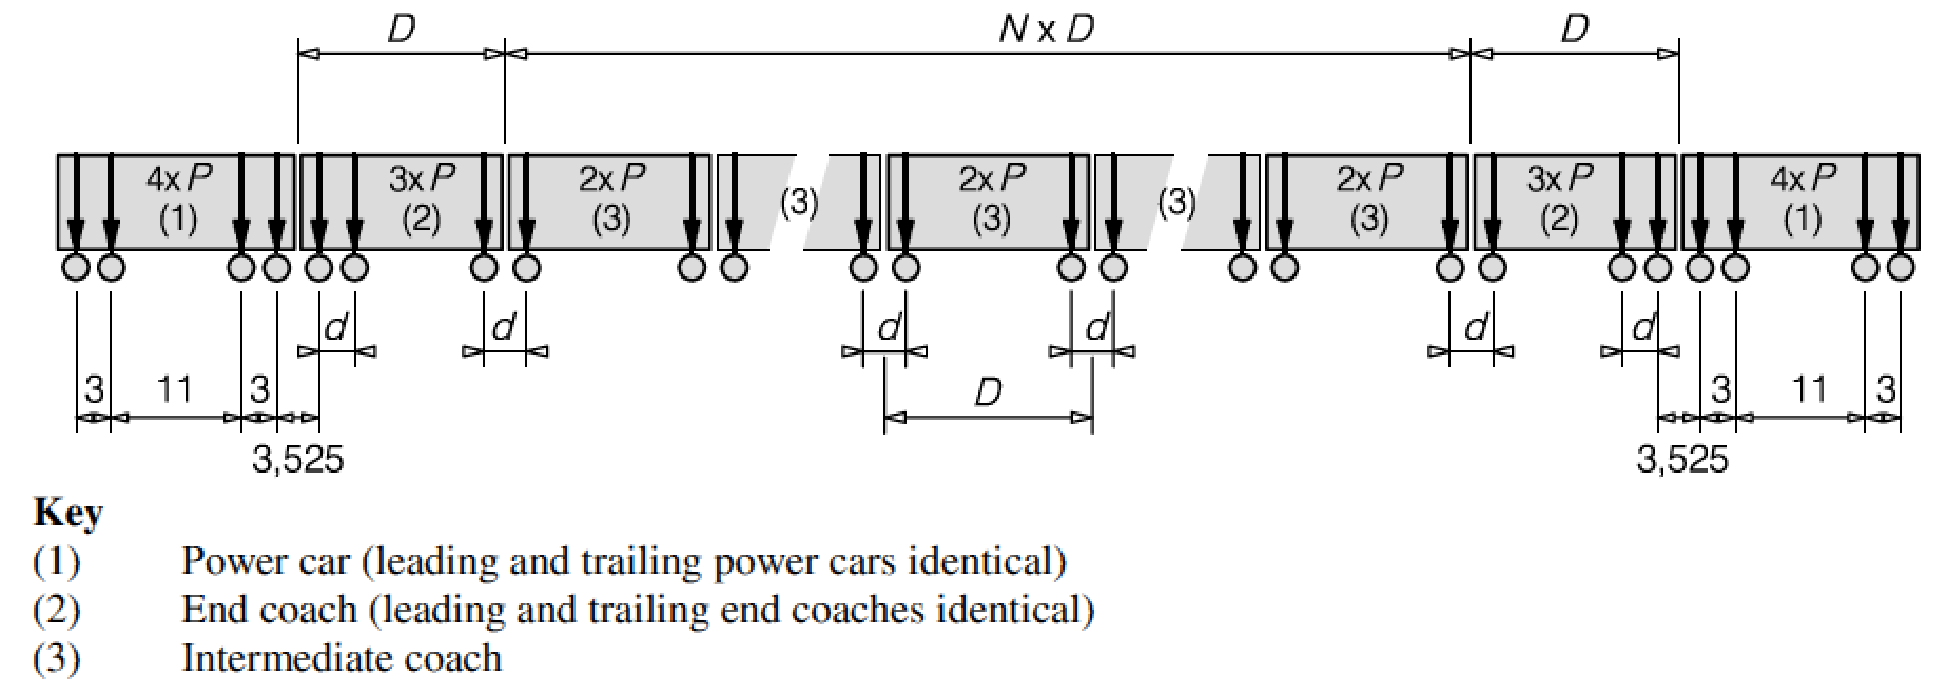
\includegraphics[width=0.8\textwidth]{hslma.pdf}
	\caption{Diagram of Universal Dynamic Train HSLM-A. Extracted from EN 1991-2\cite{EC12}}
	\label{fig:hslma}
\end{figure}

\begin{table}[h]\footnotesize
	\centering
	\begin{tabular}{p{2cm}p{2cm}p{2cm}p{2cm}p{2cm}}
		\hline
		Universal train & Number of intermediate coaches, $ N $ & Coach length $ D(m) $ & Bogie axle spacing $ d (m) $ & Point force $ P (kN) $ \\
		\hline
		A1 & 18 & 18 & 2.0 & 170 \\
		A2 & 17 & 19 & 3.5 & 200 \\
		A3 & 16 & 20 & 2.0 & 180 \\
		A4 & 15 & 21 & 3.0 & 190 \\
		A5 & 14 & 22 & 2.0 & 170 \\
		A6 & 13 & 23 & 2.0 & 180 \\
		A7 & 13 & 24 & 2.0 & 190 \\
		A8 & 12 & 25 & 2.5 & 190 \\
		A9 & 11 & 26 & 2.0 & 210 \\
		A10 & 11 & 27 & 2.0 & 210 \\			
		\hline		
	\end{tabular}
	\caption{HSLM-A, definition of ten trains. Extracted from EN1991-2\cite{EC12}}
	\label{tab:hslma}
\end{table}

\begin{figure}[h]
	\centering
	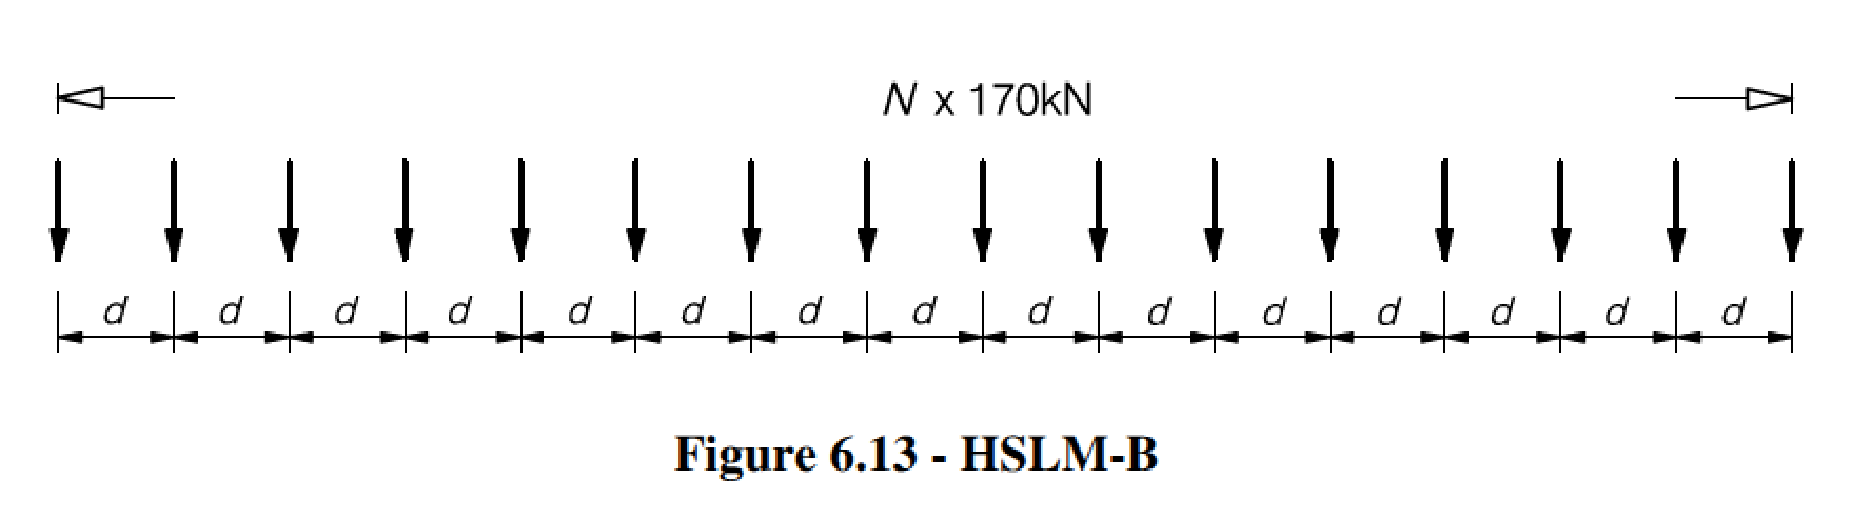
\includegraphics[width=0.8\textwidth]{hslmb.pdf}
	\caption{Diagram of Universal Dynamic Train HSLM-B. Extracted from EN 1991-2\cite{EC12}}
	\label{fig:hslmbdiagram}
\end{figure}

\begin{figure}[h]
	\centering
	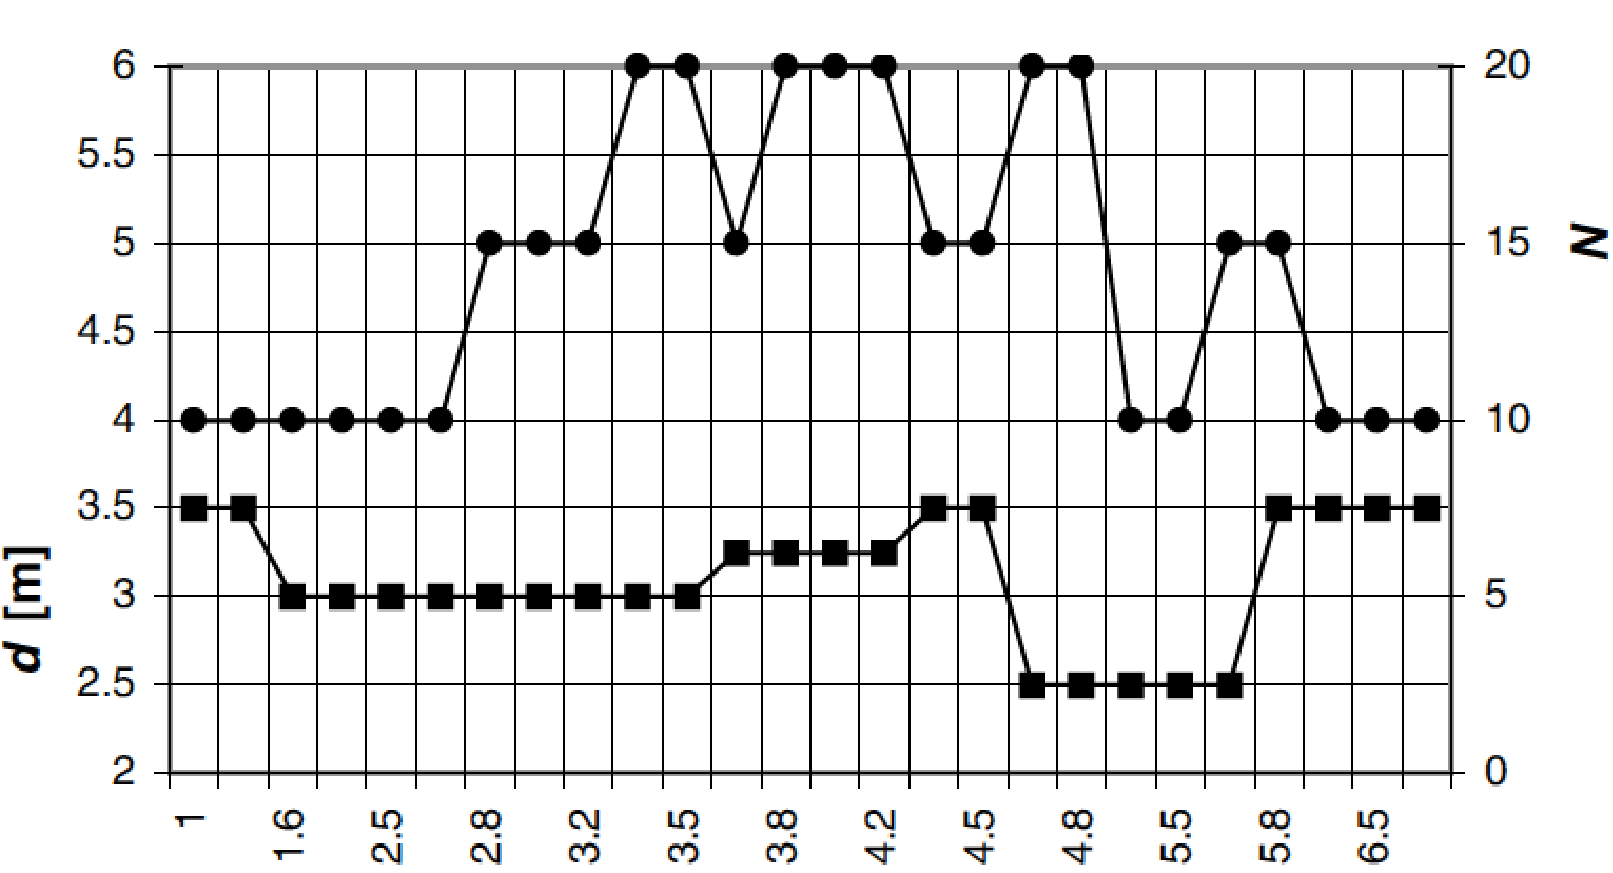
\includegraphics[width=0.8\textwidth]{hslmb2.pdf}
	\caption{Universal Dynamic Train HSLM-B. Extracted from EN 1991-2\cite{EC12}}
	\label{fig:hslmbtable}
\end{figure}

This Load Model comprises $ N $ number of point forces of 170kN at regular spacing $ d(m) $ (\ref{fig:hslmbdiagram}) where $ N $ and $ d $ are defined in Figure.~\ref{fig:hslmbtable}

Table.~\ref{hslmapplication} illustrates how HSLM-A and HSLM-B are applied and indicates the train to be used for dynamic bridge calculations.

\begin{table}[h] \scriptsize
	\begin{tabular}{lll}
		\hline
		Structural configuration & \multicolumn{2}{c}{Span} \\
		& $ L<7m $ & $ L\geq 7m $ \\
		\hline
		Simply supported span & HSLM-B & HSLM-A \\
		Continuous structure or Complex Structure & Trains A1 to A10 inclusive & Trains A1 to A10 inclusive\\
	\end{tabular}
	\caption{Application of HSLM-A and HSLM-B. Data extracted from EN 1991-2\cite{EC12}}
	\label{hslmapplication}
\end{table}

\subsection{Dynamic factor}\label{sec:dynamicfactor}
The dynamic factor $ \Phi $ takes account of the dynamic magnification of stress and vibration effects in the structure but does not take account of resonance effects.

Generally the dynamic factor $ \varPhi $ is taken as either $ \varPhi_2 $ or $ \varPhi_3 $ according to the quality of track maintenance as follows:

\begin{enumerate}[(a)]
	\item For Carefully maintained track: 
		\begin{equation}
			\varPhi_2=\dfrac{1.44}{\sqrt{L_\varPhi}-0.2}+0.82 \quad with1.00\leq \varPhi_2\leq 1.67
		\end{equation}
	\item For track with standard maintenance:
		\begin{equation}
			\varPhi_3=\dfrac{2.16}{\sqrt{L_\varPhi}-0.2}+0.73 \quad with 1.00\leq \varPhi_3\leq 2.0
		\end{equation}\\
	where $ L_\varPhi $ is the `determinant' length (length associated with $ \varPhi $ ) in metres as defined in Table 6.2, EN1991-2\cite{EC12}.
\end{enumerate}

\subsection{Static analysis}
A static analysis shall be carried out with the load models defined in Section Load Models(LM71 and where required Load Models SW/0 and SW/2). The result shall be multiplied by the dynamic factor $ \Phi $ (and if required multiplied by $ \alpha $)

\subsection{Bridge parameters}
In designers' guide\cite{calgaro2010designers}, bridge parameters on dynamic effects are discussed.

\subsubsection{Structural damping}
Structural damping is a key parameter in dynamic analysis. The magnitude of the vibrations depends heavily on structural damping, especially in proximity to resonance.

\subsubsection{Mass of the bridge}
Maximum dynamic effects occur at resonance peaks, where a multiple of the load frequency coincides with the natural frequency of the structure. Underrating the mass will lead to over-estimation of the natural frequency of the structure and of the speed at which resonance occurs.

\subsubsection{Stiffness of the bridge}
Maximum dynamic load effects are likely to occur at resonant peaks when a multiple of the frequency of loading and a natural frequency of the structure coincide. Any overestimation of bridge stiffness will overestimate the natural frequency of the structure and speed at which resonance occurs; it provides conservative results.

\subsection{Dynamic analysis}
EN 1991-2\cite{EC12} doesn't specify the method of dynamic analysing, but UIC Leaflet 776\textsuperscript{2}\cite{uic} indicates that  for normal bridges there are 4 methods of analysing(an approximate method and three simplified method). However, 776\textsuperscript{2}\cite{uic} also indicates for special structures (bridges with long spans such as bowstring bridges), have to be solved using generic finite element (FEM) programs.

Analysing using FEM programs can be very time and money consuming providing a complicated structure. Fortunately UIC Leaflet 776\textsuperscript{2}\cite{uic} is an optional reference so FEM analysing is not required in EN 1991-2 \cite{EC12}. Thus finding a simplified way of analysing complicated bridge structures is vital. The development of dynamic analysing methods will be discussed in Chapter.\ref{sec:dynamic-analysing-methods}

\subsection{Verification of the Limit States}
\cite[6.4.6.5]{EC12} proposes following principles to be followed during design:

To ensure traffic safety:
\begin{enumerate}
	\item The verification of maximum peak deck acceleration shall be regarded as a traffic safety requirement checked at the serviceability limit state for the prevention of track instability
	\item The dynamic enhancement of load effects shall be allowed for by multiplying the static loading by the dynamic factor $\varPhi$ defined in \cite[6.4.5]{EC12}. If a dynamic analysis is necessary, the results of the dynamic analysis shall be compared with the results of the static analysis enhanced by $\varPhi$ (and if required multiplied by $\alpha$ in accordance with \cite[6.3.2]{EC12}) and the most unfavourable load effects shall be used for the bridge design.
	\item If a dynamic analysis is necessary, a check shall be carried out according to \cite[6.4.6.6]{EC12} to establish whether the additional fatigue loading at high speeds and at resonance is covered by consideration of the stresses due to load effects from $\varPhi \times LM71$ (and if required $\varPhi \times Load Model SW/0$ for continuous structures and classified vertical load in accordance with \cite[6.3.2(3)]{EC12} where required). The most adverse fatigue loading shall be used in the design.  
\end{enumerate}

\subsubsection{Ultimate limit states}

\subsubsection{Serviceability limit states - traffic safety}

\paragraph{Vertical accelerations of the deck}
The maximum peak values for bridge deck accelerations, calculated along each track, shall not exceed the following design values:

\begin{enumerate}
	\item $ 3.5m/s^2 $ for ballasted track
	\item $ 5m/s^2 $ for direct fastened track with tracks and structural elements designed for high speed traffic
\end{enumerate}

Also, the range of frequencies to take into account in the determination of the dynamic response in terms of accelerations, shall not exceed the maximum of the following values:

\begin{enumerate}
	\item $30Hz$
	\item $1.5\times n_0$
	\item the frequency of the third mode of vibration of the member in study
\end{enumerate}

\paragraph{Deck twist}
The twist of the bridge shall be calculated taking into account the characteristic values of Load Model 71 as well as SW/0 or SW/2 as appropriated multiplied by $\phi$ and $\alpha$ and Load Model HSLM including centrifugal effects, all in accordance with EN1991-2, 6. 

Twist shall be checked on the approach to the bridge, across the bridge and for the departure from the bridge (see A2.4.4.1(2)P).

The maximum twist $t$ [mm/3m] of a track gauge $s$ [m] of 1.435m measured over a length of 3m(Figure\ref{fig:difinitiondecktwist}) should not exceed the values given in Table:\ref{tab:limitingvaluedecktwist}

\begin{table}[h]
	\centering
	\begin{tabular}{cc}
		\hline
		Speed range $V$ (km/h) & Maximum twist $t$ (mm/3m) \\
		\hline
		$v\leq 120$ & $t\leq t_1$ \\
		$120\leq v \leq 200$ & $t\leq t_2$ \\
		$v>200$ & $t\leq t_3$ \\
		\hline
	\end{tabular}
	\\
	\raggedright{Note The values for $t$ may be defined in the National Annex.\\ The recommended values for the set of $t$ are:\\ $t_1=4.5$\\$t_2=3.0$\\$t_3=1.5$\\Values for a track with a different gauge may be defined in the National Annex}
	\caption{Limiting Values of deck twist}
	\label{tab:limitingvaluedecktwist}
\end{table}
	
\begin{figure}[h]
	\centering
	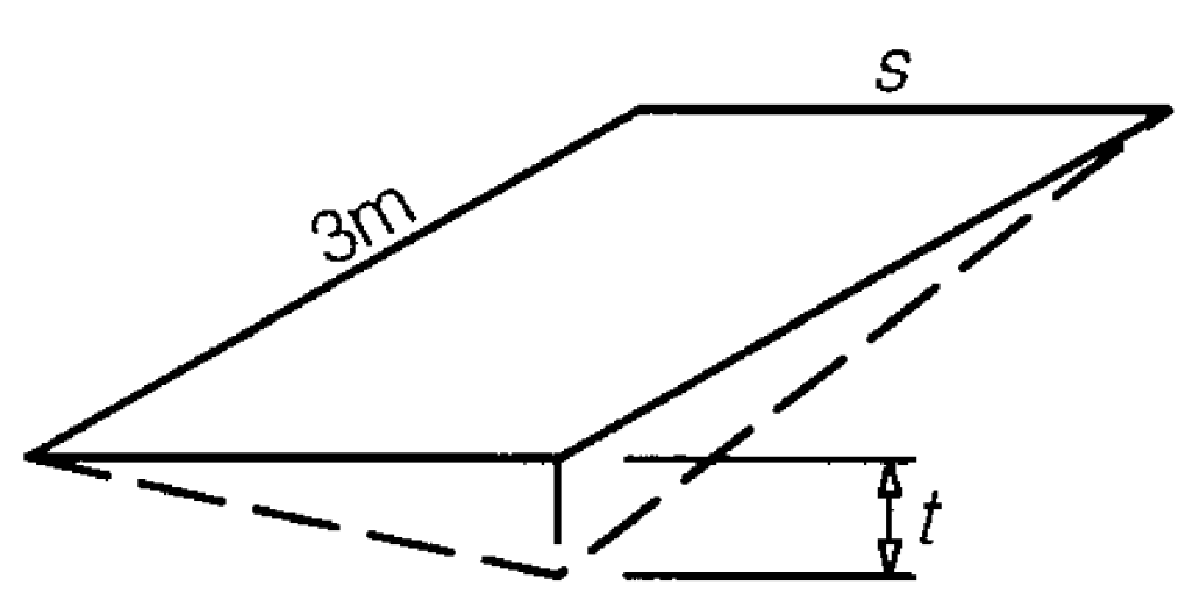
\includegraphics[width=0.8\textwidth]{definitiondecktwist.pdf}
	\caption{Definition of deck twist. Extracted from \cite[Figure A2.1]{1990a2}}
	\label{fig:difinitiondecktwist}
\end{figure}

\paragraph{Vertical deformations}
For all the structures configurations, loaded with the classified characteristic vertical LM 71, or with the models SW/0 and SW/2 if required, the maximum  total vertical deflection measured along any track due to railway traffic actions should not exceed $L/600$. The angular rotations at the end of decks, represented in Figure.\ref{fig:difinitionangularrotations} , in the vicinity of expansion devices, switches and crossings, should be verified.

\begin{figure}[h]
	\centering
	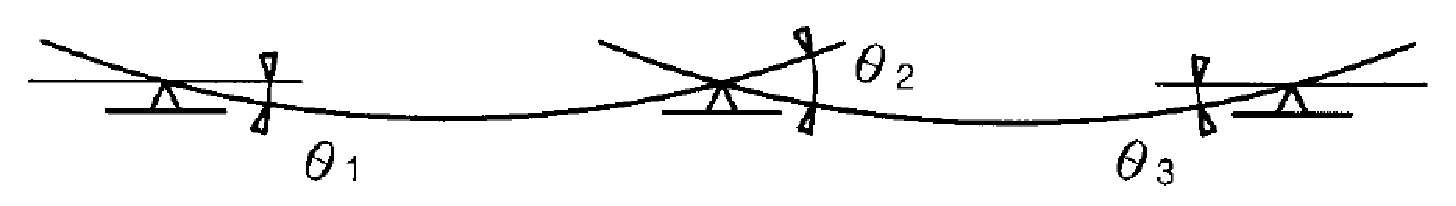
\includegraphics[width=0.8\textwidth]{definitionangularrotations.pdf}
	\caption{Definition of anular rotations at the end of the decks. Extracted from \cite[Figure A2.2]{1990a2}}
	\label{fig:difinitionangularrotations}
\end{figure}

\paragraph{Transverse deformations and vibrations}\label{sec:Transverse-deformations-and-vibrations}
\cite[A2.4.4.2.4]{1990a2}  proposed that transverse deformation and vibration of the deck shall be checked for characteristic combinations of Load Model 71 and SW/0 as appropriate multiplied by the dynamic factor $\phi$ and $\alpha$ (or real train with the relevant dynamic factor if appropriate), wind loads, nosing force, centrifugal forces in accordance with \cite[6]{EC12} and the effect of a transverse temperature differential across the bridge.

The transverse deflection $ \delta_h $ at the top of the deck should be limited to ensure:

\begin{enumerate}
	\item a horizontal angle of rotation of the end of a deck about a vertical axis not greater than the values given in Table.~\ref{tab:maximumhorizontalrotation} , or
	\item the change of radius of the track across a deck is not greater than the values in Table.~\ref{tab:maximumhorizontalrotation} , or
	\item at the end of a deck the differential transverse deflection between the deck and adjacent track formation or between adjacent decks does not exceed the specified value
\end{enumerate}

\begin{table}[h]
	\centering
	\begin{tabularx}{0.8\textwidth}{cXcc}
	\hline
	Speed range V(km/h) & Maximum horizontal rotation(radian) & \multicolumn{2}{c}{Maximum change of radius of curvature}\\
	& & Single deck & Multi-deck bridge\\
	\hline
	$ V\leq 120 $ & $ \alpha_1 $ & $ r_1 $ & $ r_4 $ \\
	$ 120\leq V \leq 200 $ & $\alpha_2 $ & $r_2$ & $ r_5 $ \\
	$V>200$ & $ \alpha_3 $ & $r_3$ & $r_6$\\
	\hline
	\end{tabularx}
	\\
	NOTE 1 The change of the radius of curvature may be determined using:
			$$ r = \frac{L^2}{8 \delta_h}$$
			
	NOTE 2 The transverse deformation includes the deformation of the bridge deck and the substructure(including piers, piles and foundations).
			
	NOTE 3 The values for the set of $\alpha_i$ and $r_i$ may be defined in the National Annex. The recommended values are:
			
	$ \alpha_1 = 0.0035$; $\alpha_2=0.0020$; $\alpha_3=0.0015$;
			
	$ r_1  =1700$; $r_2=6000$; $r_3=14000$;
			
	$ r_4 = 3500$; $r_5 = 9500$; $ r_6 = 17500$
	
	\caption{Maxiumum horizontal rotation and maximum change of radius of curvature}
	\label{tab:maximumhorizontalrotation}
\end{table}

The first natural frequency of lateral vibration of a span should not be less than $f_{h0}$. The value for $f_{h0}$ may be defined in the National Annex. The recommended value is: $f_{h0}=1.2 Hz$

\paragraph{Longitudinal displacements}
For rails on the bridge and on the adjacent abutment, the permissible additional rail stresses due to the combined response of the structure and the track, due to variable actions, should be limited to the following design values:

\begin{enumerate}
	\item Compression: $72KN/mm^2$
	\item Tension: $92KN/mm^2$
\end{enumerate}

\begin{figure}[p]
	\centering
	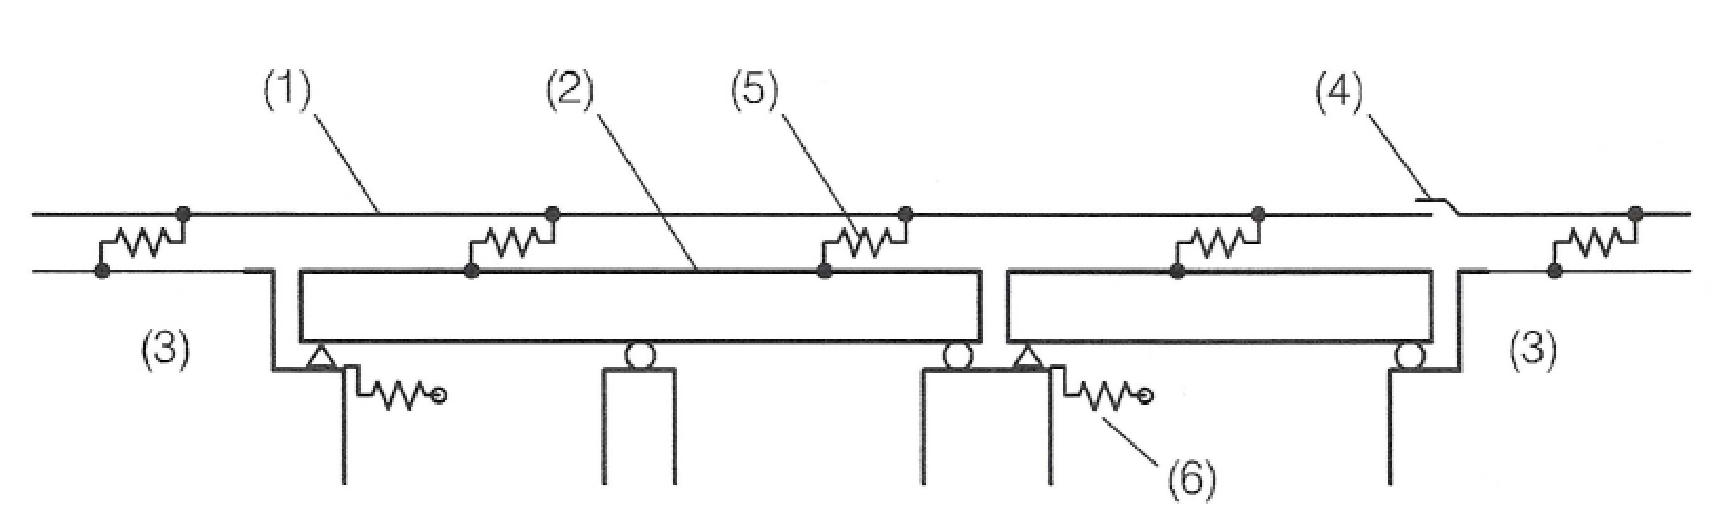
\includegraphics[width=0.8\textwidth]{modeltrackstructure.pdf}
	\caption{Model of a track/structure system. Extracted from \cite[Figure 6.19]{EC12}}
	\label{fig:modeltrackstructure}
\end{figure}

\begin{figure}[p]
	\centering
	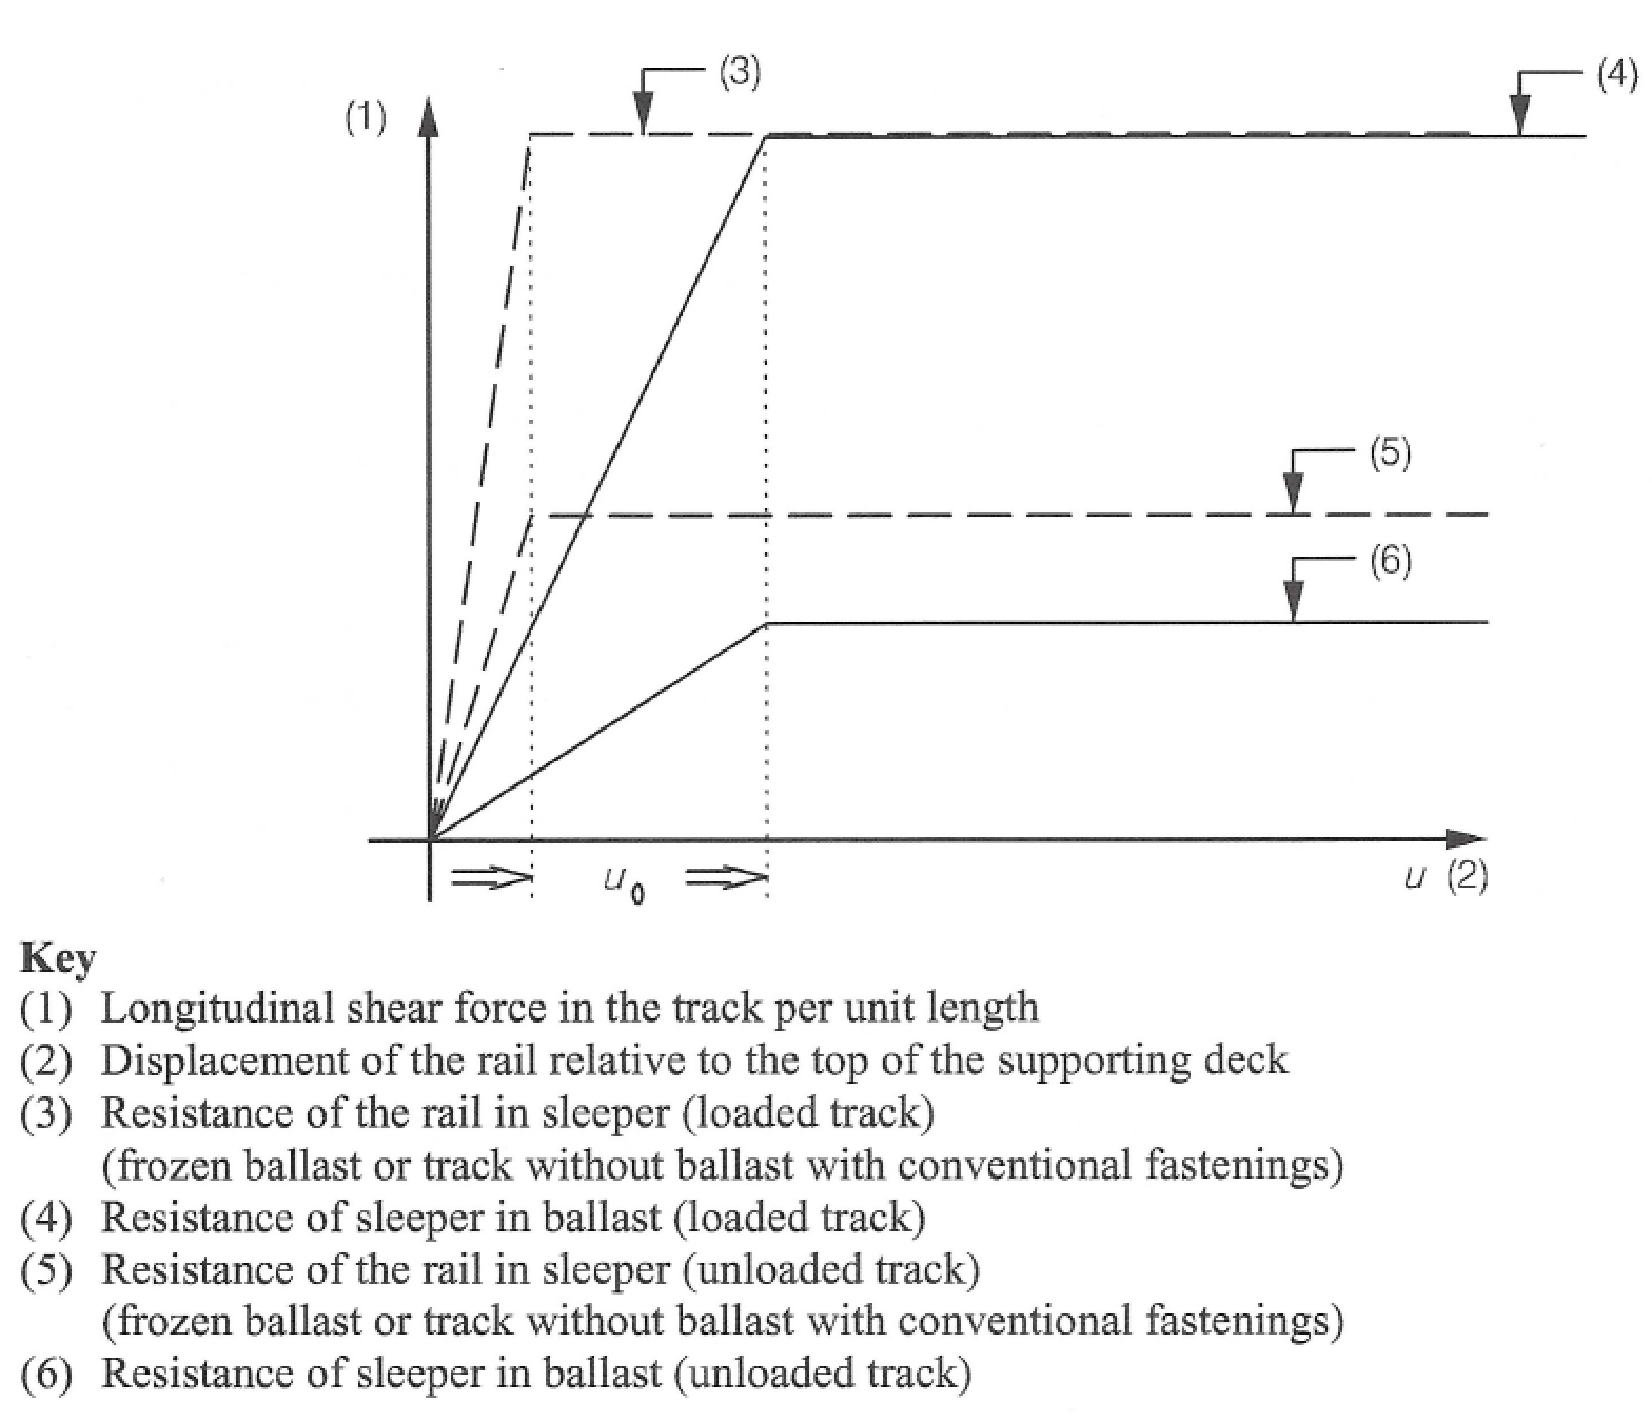
\includegraphics[width=0.8\textwidth]{variationlongitudinalshearforce.pdf}
	\caption{Variation of longitudinal shear force with longitudinal track displacement for one track. Extracted from \cite[Figure 6.20]{EC12}}
	\label{fig:variationlongitudinalshearforce}
\end{figure}

When determining the combined response of track and structure to traction and braking forces, these forces should not be applied on the adjacent embankment unless a complete analysis is carried out considering the approach, passage over and departure from the bridge of rail traffic on the adjacent embankments to evaluate the most adverse load effects.

For the determination of load effects in the combined track/structure system a model based upon Figure\ref{fig:modeltrackstructure} may be used where the longitudinal load/displacement behaviour of the track or rail supports may be represented by the relationship shown in Figure.\ref{fig:variationlongitudinalshearforce}.

Model in Figure\ref{fig:modeltrackstructure} is very important to evaluate the security of the track structure and not the structural security. High track deformations can lead to unfavourable effects for the structure and for vehicles when these are crossing the bridge.

\subsubsection{Serviceability limit states - passenger comfort}

For these type of verifications \cite{1990a2} defines the limiting values for the maximum vertical deflection for passenger comfort, as following:

\begin{enumerate}
	\item Comfort criteria
	\item Deflection criteria for checking passenger comfort
	\item Requirements for a dynamic vehicle/bridge interaction analysis for checking passenger comfort
\end{enumerate}

Passenger comfort depends on the vertical accelerations, $b_v$, inside the coach. These levels of comfort limiting values for the vertical accelerations are presented in Table.\ref{recommendedaccelerationsvalues}

\begin{table}[h]
	\centering
	\begin{tabular}{cc}
		\hline
		Very good & $1.0m/s^2$ \\
		Good & $1.3 m/s^2$ \\
		Acceptable & $2.0m/s^2$\\
		\hline
	\end{tabular}
	\caption{Recommended accelerations values to ensure the respective levels of comfort. Extracted from \cite[Table A 2.9]{1990a2}.}
	\label{recommendedaccelerationsvalues}
\end{table}

\begin{figure}[h]
	\centering
	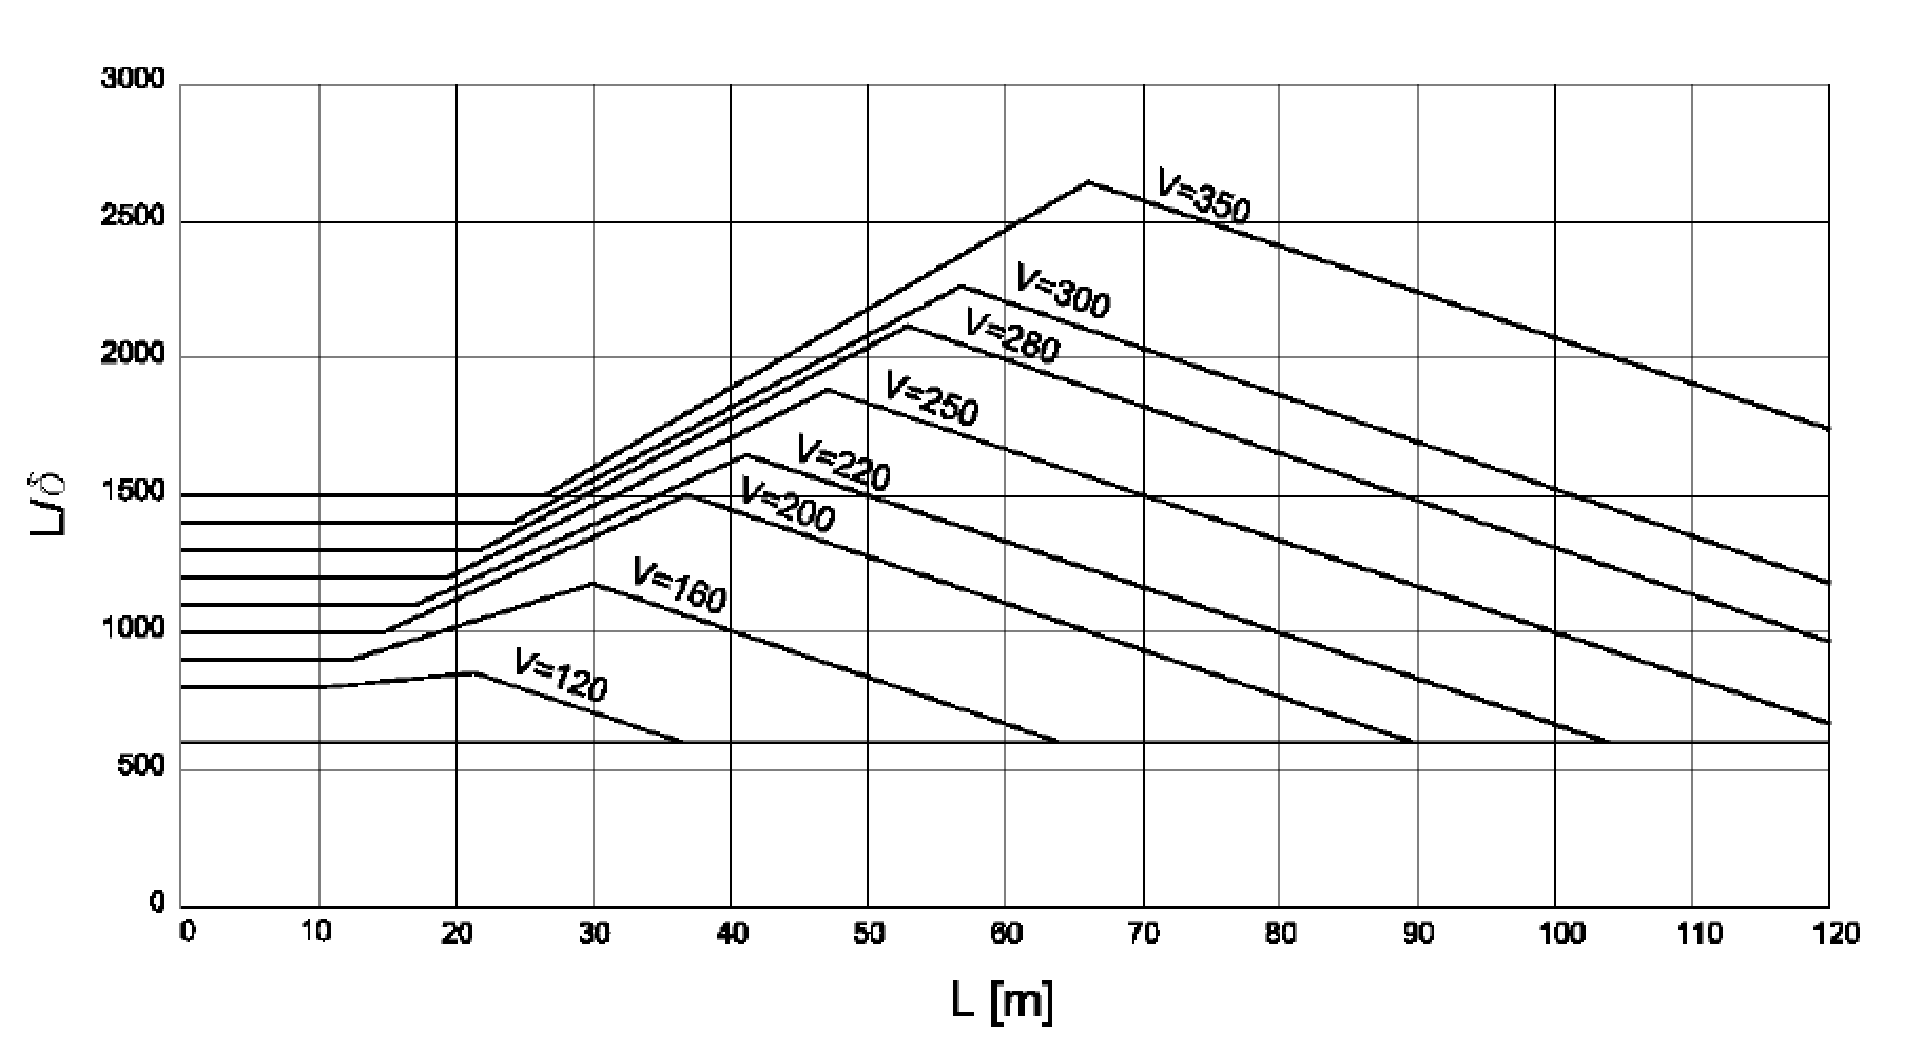
\includegraphics[width=0.8\textwidth]{recommendedlevelofcomfort.pdf}
	\caption{Maximum permissible vertical deflection $\delta$ for railway bridges with 3 or more successive simply supported spans corresponding to a permissible vertical acceleration of $b_v=1m/s^2$ in a coach for speed $V$[km/h]. Extracted from \cite[Figure A2.3]{1990a2}}
	\label{fig:recommendedlevelofcomfort}
\end{figure}

In order to limit vertical vehicle acceleration, being the limits defined in Table\ref{recommendedaccelerationsvalues},vertical displacements should be less than the maximum permissible vertical deflection, $\delta$, obtained from Figure\ref{fig:recommendedlevelofcomfort}. These values are expressed in function of the span length $L$[m], and train speed $V$[km/h], which is valid only for railway bridges with three or more successive simply supported spans. Alternatively these accelerations can be determined considering the vehicle-structure interaction dynamic analysis.

Additionally, the limiting values of $L/\delta$, defined in Figure\ref{fig:recommendedlevelofcomfort} are given for $b_v=1.0m/s^2$.

Vertical deflections should be determined with the LM 71 model multiplied by the factor $\phi$ and adopting $\alpha=1$, being only one track loaded for the case of bridges with two or more tracks.

\subsection{Principal supplementary checks}
\subsubsection{Verification of maximum peak deck acceleration along each track}
\subsubsection{Verification of whether the calculated load effects from high-speed rail traffic, including HSLM on high-speed interoperable routes, are greater than those of normal rail traffic loading(LM71''+''SW/0)}
\subsubsection{Additional verification for fatigue where dynamic analysis is required}
\subsubsection{Verification of limiting values for the maximum vertical deflection for passenger comfort}

\subsection{Diagram of general procedures}
By summarizing Eurocode several steps of calculation are extracted as following, arranged in chronological order.

\begin{enumerate}
	\item  Follow the conceptual check to avoid unsafe designs
	\item  Follow the logic diagram in Figure~\ref{fig:logicdiagram} to check whether dynamic analyses are required 
	\item  Find the appropriate train models, including 
	\begin{enumerate}
		\item-Hypotheses relating to rolling stock
		\item-Rolling stock for interoperability
		\item-Load models HSLM
		\item-Load distribution
		\item-Load combinations and partial factors
		\item-Train speeds to be considered
	\end{enumerate}
	\item Perform the static analyses
	\item  Examine bridge parameters, including
		\begin{enumerate}
			\item-Structural damping
			\item-Mass of the bridge
			\item-Stiffness of the bridge
		\end{enumerate}
	\item Perform the dynamic analyses
	\item  Principal supplementary design checks, including
	\begin{enumerate}
		\item-Verification of maximum peak deck acceleration along each track
		\item-Verification of whether the calculated load effects from high-speed rail traffic, including HSLM on high-speed interoperable routes, are greater than those of normal rail traffic loading(LM71''+''SW/0)
		\item-Additional verification for fatigue where dynamic analysis is required
		\item-Verification of limiting values for the maximum vertical deflection for passenger comfort
	\end{enumerate}
	\item The results of the dynamic analysis shall be compared with the results of the static
analysis multiplied by the dynamic factor $\varPhi$ in 6.4.5 The most unfavourable values of the load effects shall be used. 
\end{enumerate}

\section{Dynamic analysing methods}\label{sec:dynamic-analysing-methods}
There are several dynamic analysing methods developed in Europe over time since Eurocodes don't specify what method to be used during dynamic analysing. These methods differ from each other in the level of calculation complexity. For example, Dynamic train signature method is a good solution for simple structures with well-known train types since it cost less time and effort. On the other hand, Train-vehicle method is an inevitable process for some complicated bridge structures thanks to its wide applicability. However, generally, Train-vehicle method is much more time and money consuming. In following paragraphs, some state-of-art dynamic analysing methods will be reviewed.


\subsection{Method based on impact factor}

\subsection{Method based on dynamic train signature}
As mentioned in \cite[A.4.3]{uic}, the dynamic signature of a train is obtained by breaking down the load diagram of a train in Fourier series and by extrapolating it to the natural modes. It represents the dynamic excitation features of the train and is independent of the characteristics of the structure. The signature depends on axle spacing and loads only. However, newly developed Train dynamic signature method like LIR method takes structure characteristics into account, giving more applicable solutions for specific bridge projects.

Train dynamic signature is a useful method of producing quick analyses on resonance characteristics of the vehicle-bridge systems. The method is especially effective for simple bridge structures.

\subsubsection{DER method}

DER = Decomposition of the Resonance Excitation

The development used in DER method begins from the analysis of the frequency of excitation produced by a train of moving loads. This method is based in the following assumptions:

\begin{enumerate} [-]
	\item Applicable only on statistically determined bridges
	\item For the analysis of statistically determined bridges, is considered that the dynamic response is significantly represented by the first mode of vibration
\end{enumerate}

The development of the method is summarised as follows:

\begin{enumerate}
	\item Reduce the response of a statistically determinate beam to a single degree of freeedom system
	\item Decomposition of the dynamic response of the bridge, in Fourier series;
	\item Consideration of the term which corresponds to the condition of resonance frequencies.
\end{enumerate}

The maximum accelerations at the midspan of the beam for a certain speed, is given as follows:

\begin{equation}
	\ddot{y}(t)\leq C_t\cdot A(L/\lambda)\cdot G(\lambda)
\end{equation}

where the first factor is a constant that depends from bridge characteristics:

\begin{equation}
	C_t=\dfrac{8\pi f_0^2}{K}=\dfrac{4}{\rho\pi L}  
\end{equation}

The second factor is a function called dynamic influence line:

\begin{equation}
	A(L/\lambda )= \bigg\vert\dfrac{\cos (\pi L/\lambda)}{(2L/\lambda)^2-1} \bigg\vert
\end{equation}

and the third factor represents the train dynamic signature, defined as follows:

\begin{equation}
	G(\lambda)=\sqrt{[\sum_{k=1}^N F_k\cos(\dfrac{2\pi x_k}{\lambda})]^2+[\sum_{k=1}^N F_k \sin(\dfrac{2\pi x_k}{\lambda})]^2}\cdot (1-e^{-2\pi \xi \dfrac{x_N}{\lambda}})\cdot \dfrac{L}{\xi x_N}
\end{equation}

\subsubsection{LIR method}
LIR method is based on residual influence line. It is applicable only on statistically determined bridges, too. The solution of the displacements and accelerations in the midspan, of the simply supported beam, is developed by \citeauthor{dominguez2001dinamica}. The solution is given as follows:

\begin{equation}
	\centering
	y_{max}=C_{desp}\cdot A(r) \cdot G(\lambda)
\end{equation}

\begin{equation}
	\ddot{y}_{max}=C_{acel}\cdot A(r) \cdot G(\lambda)
\end{equation}

with,

\begin{equation}
	C_{desp} = \frac{1}{M\omega_0^2},
	C_{acel} = \frac{1}{M}
\end{equation}

The factor $ A(r) $ is the dynamic influence line, give as:

\begin{equation}
	A(r)=\frac{r}{1-r^2}\sqrt{e^{-2\xi \frac{\pi}{r}}+1+2\cos (\frac{\pi}{r})e^{-2\xi \frac{\pi}{r}}}
\end{equation}

with $ r=\lambda/2L $.

$G(\lambda)$ is named train dynamic signature, depending from train characteristics and from the damping coefficient of the structure, give as follows:

\begin{equation}
\end{equation}

To make $G(\lambda)$ representative for the maximum response, maximum value of $G(\lambda)$ for each different subtrain is considered the value of $G(\lambda)$

\begin{equation}
	G(\lambda) = \max_{i=1}^{N} \sqrt{[\sum_{x_1}^{x_i}F_i\cos (2\pi \delta_i) e^{-2\pi \xi \delta_i}]^2+[\sum_{x_1}^{x_i}F_i \sin (2\pi \delta_i) e^{-2\pi \xi \delta_i}]^2}
\end{equation}

\begin{figure}[h]
	\centering
	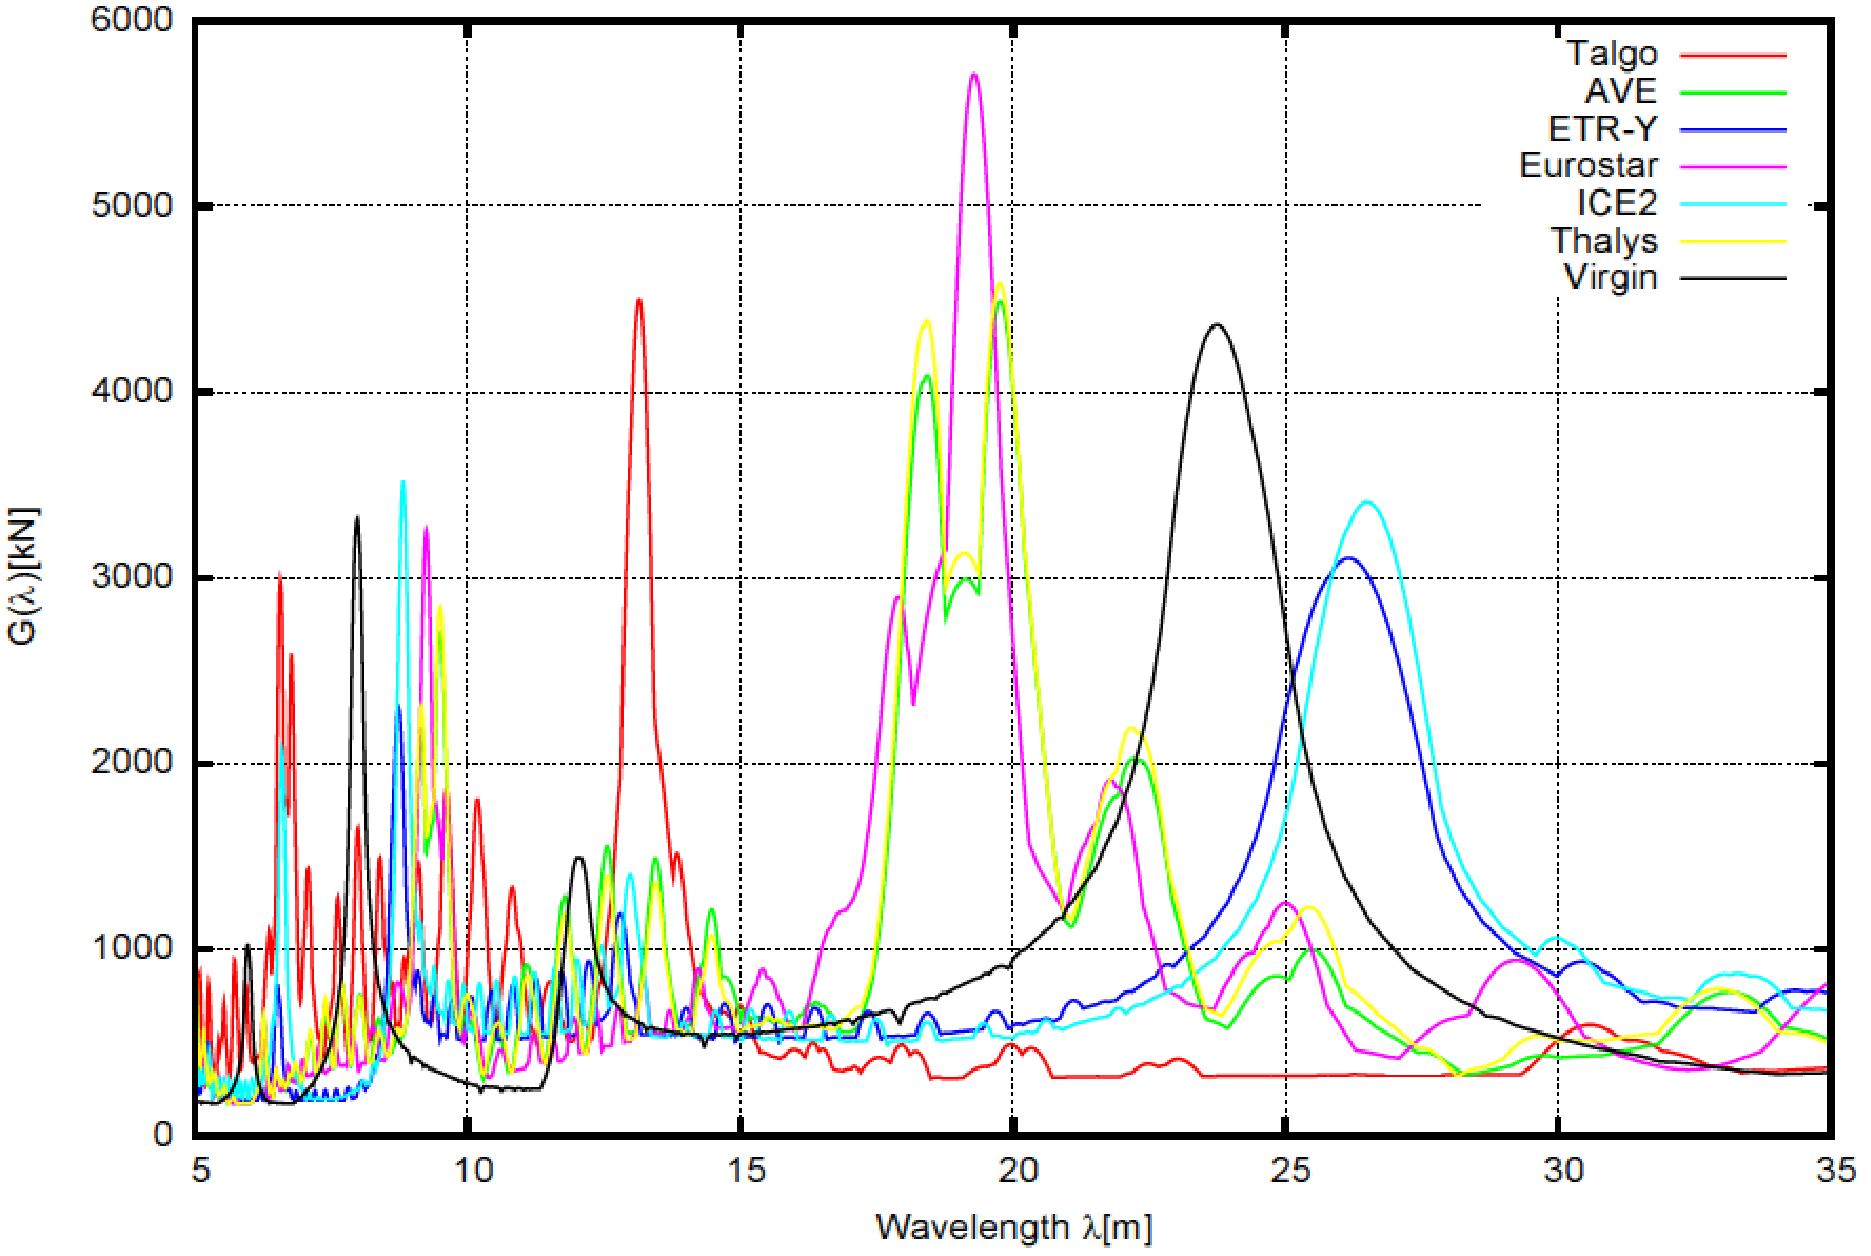
\includegraphics[width=0.6\textwidth]{trainsig.pdf}
	\caption{Train dynamic signatures for the seven real trains, considering a damping value of $\xi = 0.00$. Extracted from \cite[Figure 2.20]{da2007dynamic}}
	\label{trainsig}
\end{figure}

\subsection{Methods based on finite element models}
Finite element methods are the most applicable methods available. The methods are based on direct time integration.

\subsubsection{Direct time integration methods}
General equation of motion for a SDOF system can be given in following form:

\begin{equation}
	\boldsymbol{M\ddot{d}}+\boldsymbol{C\dot{d}}+\boldsymbol{Kd}=\boldsymbol{f}(t)
\end{equation}

where $\boldsymbol{M}$ is the mass matrix, $ \boldsymbol{c} $ is the damping matrix, $ \boldsymbol{K} $ is the stiffness matrix, $ \boldsymbol{f}(t) $ is the vector of external loads and $ \boldsymbol{d} $ the unknown vector of nodal displacements. 

Direct time integration method is the principle of finite element models. Due to the expected huge amount of calculation, computers are used to process time integration calculations. Thanks to the reliability and efficiency of computers, there are more and more project done with the help of computer FEM software nowadays.

\subsubsection{Modelling a train of moving loads}
The method of modelling spatial moving loads in FEM software is applying load histories in each convenient node. At a certain time-step, a load F, whose magnitude depending linearly on the distance from the axle to the node, is assigned to each node if the load axis is above an element that contains the node. The procedure is outlined in Figure.\ref{fig:movingloads}.

\begin{figure}[h]
	\centering
	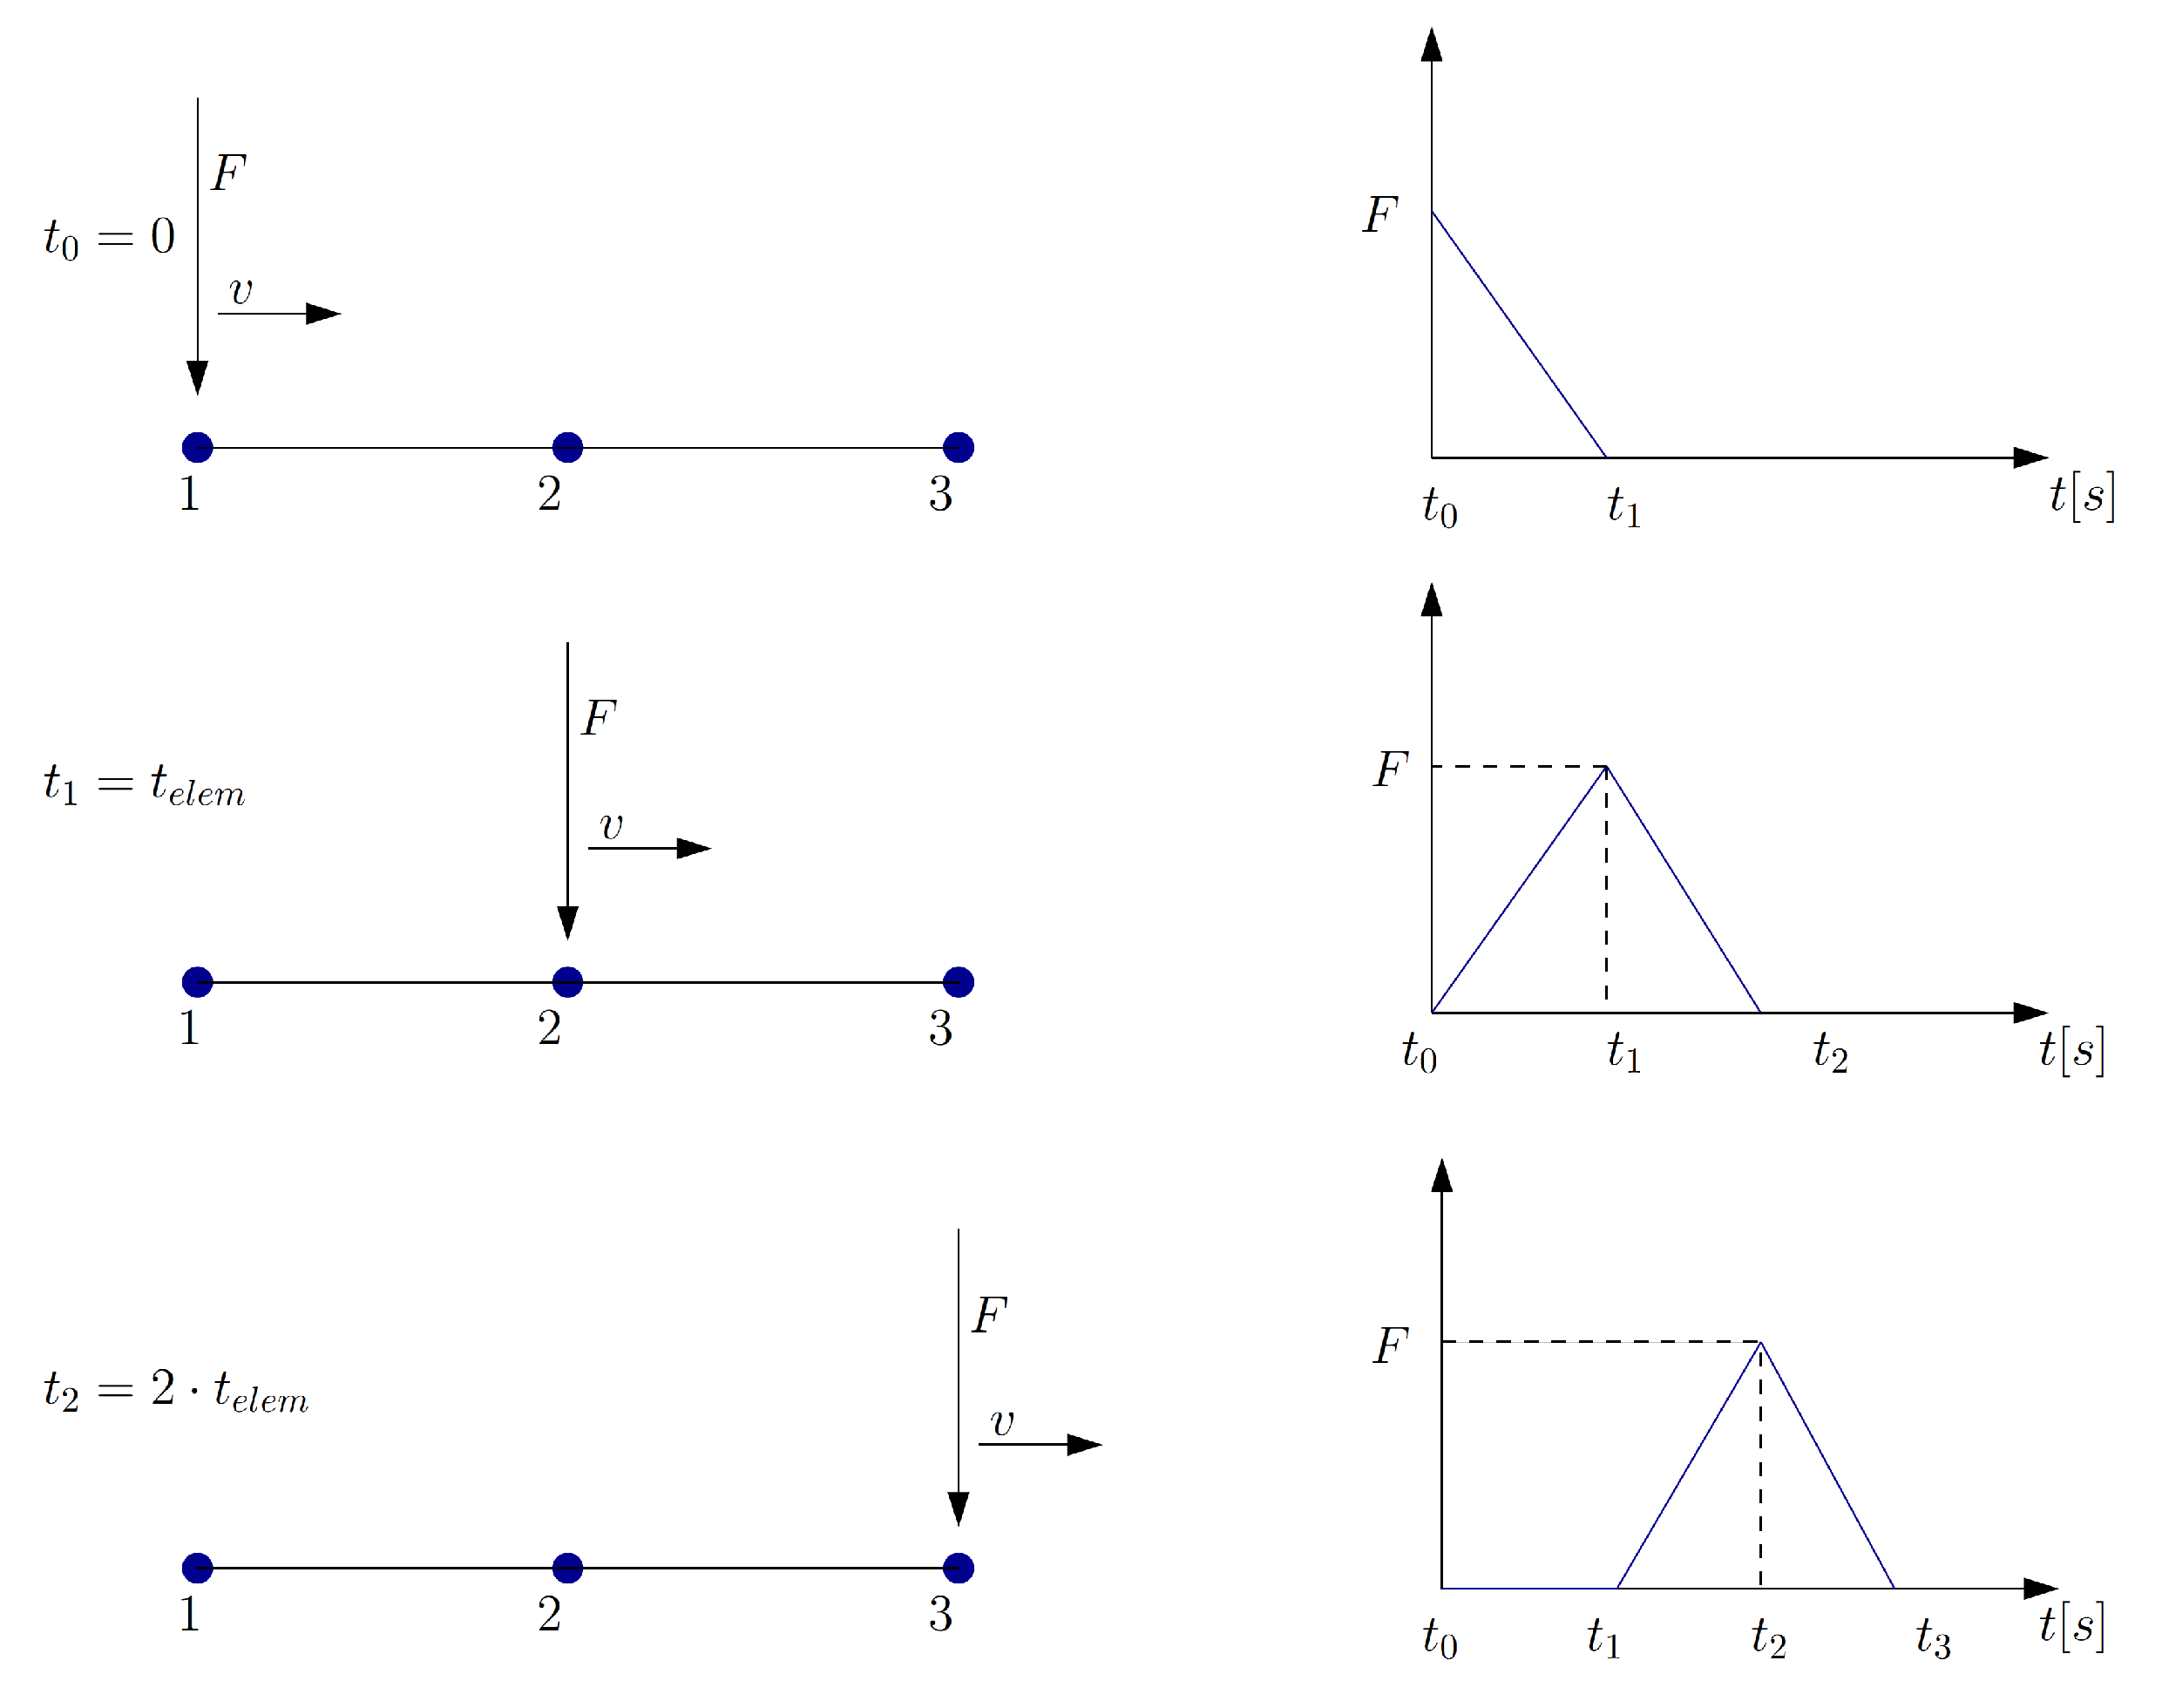
\includegraphics[width=0.8\textwidth]{movingloads.pdf}
	\caption{Nodal force time history definition for a single moving load $F$, with speed $v$. Extracted from \cite[Figure 2.15]{da2007dynamic}}
	\label{fig:movingloads}
\end{figure}

\subsection{Analytical methods based on modal analysis}
Modal analysis is the study of the dynamic properties of structures under vibrational excitation. Applied on railway bridge structures, the analysis can be simple if the bridge is modelled as a simply supported beam.

\subsubsection{Modal analysis of a simply supported beam}
blahblahblahblahblah stuff

\blindtext

Contents to be added

\subsubsection{Modes of vibration}

\blindtext

\subsubsection{Number of modes of vibration to consider in the analysis}

\blindtext


\subsection{Method based on vehicle-Structure interaction dynamic analysis}\label{sec:tds}
Different from point load models, vehicle-structure models takes suspension systems of train vehicles into account, providing associations between train carriage and structure. Impact of suspension system vibration on bridge structure can be neglected when the span of the bridge is comparably small since there's little chance for suspension system and bridge to resonant. As the span of bridges increase, the first vertical/transverse natural frequency of bridge can decrease into the natural frequency range of train suspension system. This means long-span bridges can resonant with train suspension system. To study the effects related to train suspension system, vehicle-structure interaction method is developed. 

A general model for a conventional coach on two bogies are shown in Figure.\ref{fig:vehicle-structure}, including the stiffness and damping $(K_P,c_P)$ of the primary suspension of each axle, the secondary suspension of the bogies $(K_s,c_s)$, the unsprung mass of the wheels $(M_w)$, the bogies $(M_b, J_b)$, and the vehicle body $(M,J)$. Similar models may be developed for articulated or regular trains.

\begin{figure}[h]
	\centering
	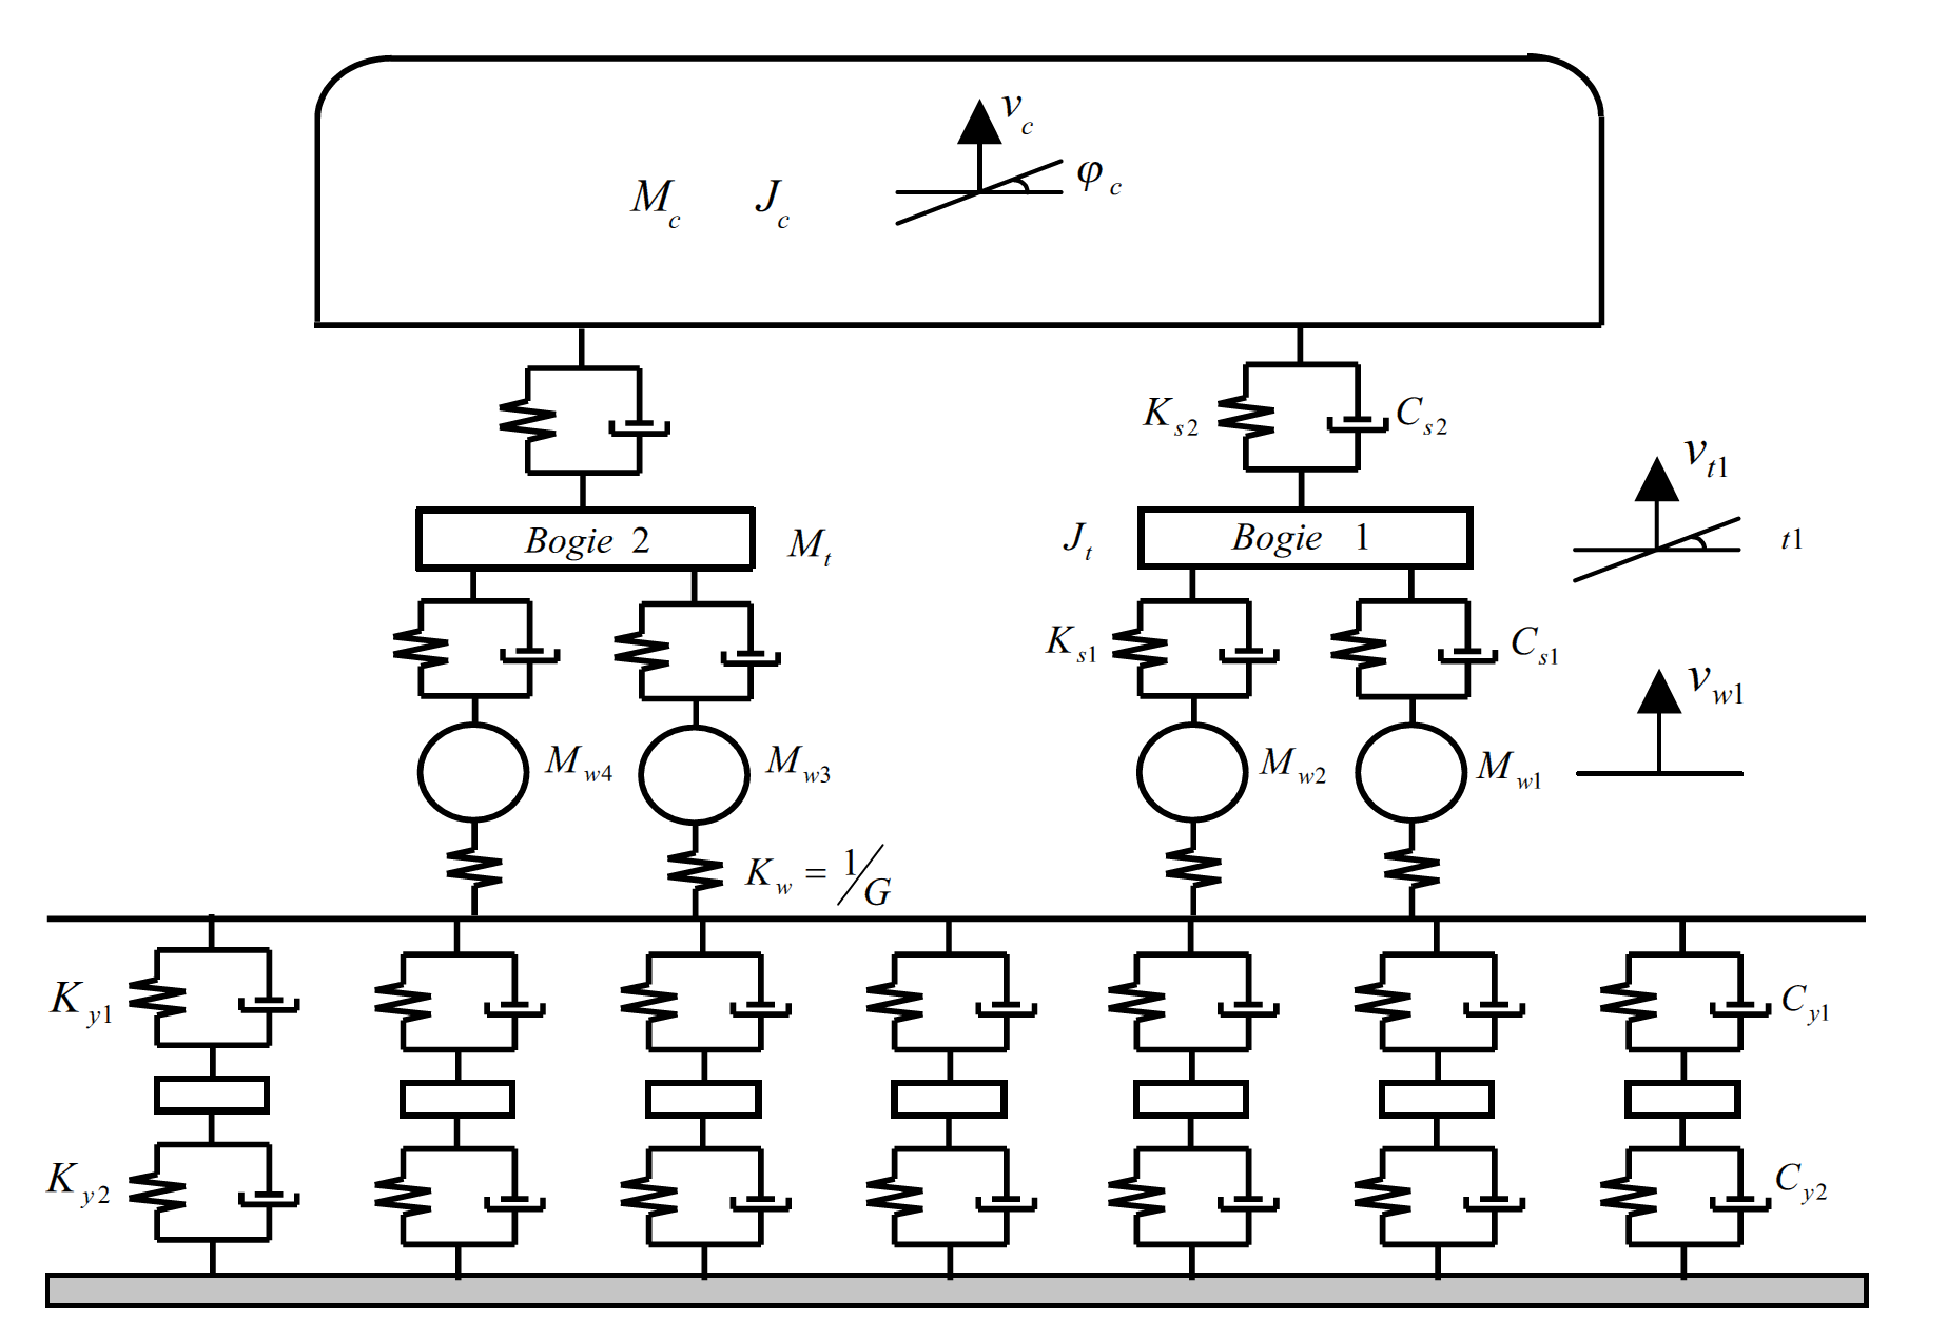
\includegraphics[width=0.8\textwidth]{vehicle-structure.pdf}
	\caption{Model for analysis of vehicle-structure system. Extracted from \cite[Figure 12]{lei2002analyses}}
	\label{fig:vehicle-structure}
\end{figure}

Sometimes more simplified model , represented by one mass, one spring and one damper per bogie can be considered, depending on the purpose of the analysis. See Figure\ref{fig:simplified-vehicle-structure} for example.

\begin{figure}[h]
	\centering
	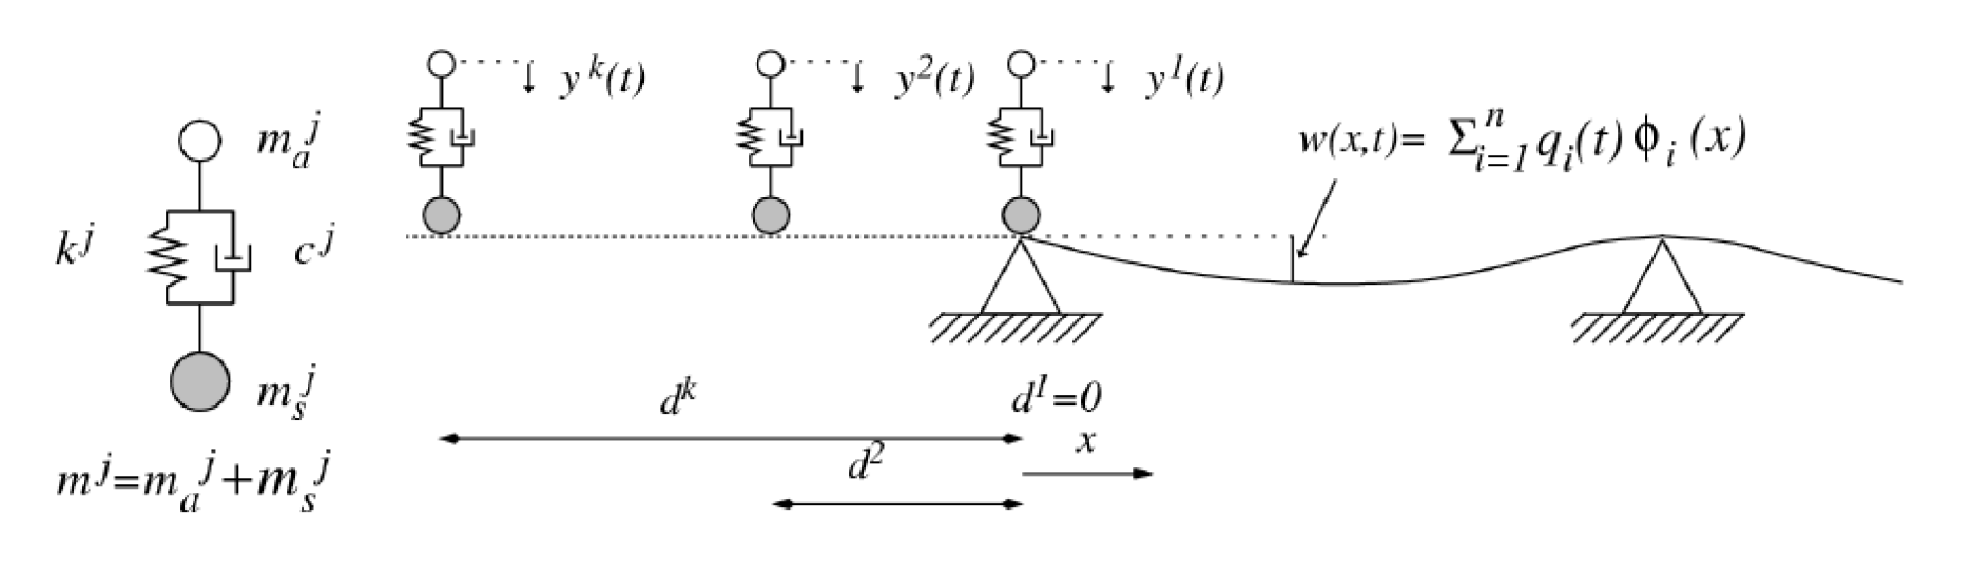
\includegraphics[width=0.8\textwidth]{simplifiedvehiclestructure.pdf}
	\caption{Load train with vehicle-bridge interaction: simplified interaction model and variables definition. Extracted from \cite[Figure15]{lei2002analyses}}
	\label{fig:simplified-vehicle-structure}
\end{figure}


%!TEX root = first try.tex

% \chapter{Background research for Criterion on Lateral Dynamics of Railway Bridges in Eurocode 1991-2}

% Eurocode is made by committees consist of experts from a variety of engineering fields. During the creating of Eurocode, it is believed that committee member will refer to existing scientific research to base code contents on. Since there isn't any explanation nor description for 1.2Hz criterion, this chapter aims to discover the supporting research behind this criterion. 

% Quoting mr. Paul Vos, one of the committee member composing Eurocode 1991-2 who is also a committee member of UIC ERRI D181 research committee, said a majority of the criteria/requirements regarding railway infrastructures are extracted from researching fruits of UIC. UIC stands for International Union of Railways. It regulates railway vehicle, infrastructure and maintenance standard for member countries all over the world. My investigation starts from reports created by ERRI, a scientific research department under UIC.

% \section{ERRI reports investigation}
% ERRI reports are created by ERRI committees, which are categorized into research topics. For example, committee D181, investigated lateral forces that acting on railway bridges. Among reports created by D181, origin of 1.2Hz criterion is found in RP6. 

% \subsection{Supporting report D181 RP6}\label{sec:1.2hz}

% Evidence of \cite{d181} is the origin of \cite[A.2.4.4.2.4(3)]{EC12} is found in \cite[p4.2: Lateral Frequencies]{d181}:

% In order to avoid the phenomena of lateral resonance in vehicles, the first natural frequency of lateral vibration of the span $f_{lt}$ such that:

% \begin{equation}
% f_{lt} \geq 1.2Hz
% \end{equation}

% The statement exactly coincides with criterion A.2.4.4.2.4(3) in Eurocode 1991. It is sufficient to acknowledge D181 RP6 as the origin of criterion A.2.4.4.2.4(3) because this report is created by UIC.

% The value of frequency limit, 1.2Hz is explained in \cite[p3.2: Criterion 2]{d181}:

% \begin{quote}
% To avoid the occurrence of resonance in the lateral motion of the vehicles due to the lateral motion of the bridge, a limit value lower than the first natural frequency $f_1t$ of the lateral vibration of the span studied should be fixed. The natural frequency for lateral movements is between 0.5 and 0.7 Hz for coaches and between 0.7 and 1 Hz for locomotives. We therefore propose a safety margin $F_{lt} \geq 1.2Hz$
% \end{quote}

% Till now, the origin of vehicle data involved in above explanation remains unknown. Since UIC publishes train vehicle standards to all its members including European Union, it is reasonable to believe researcher of Committee D181 use internal information of UIC to get the frequency of lateral vehicle moving.

% From this statement we can conclude that the background of 1.2Hz criterion is Eurocode 1991-2 avoids bridges having a first lateral natural frequency that falls between lateral vibrating frequency of running train. But this criterion can be judged as too conservative since it covers a frequency bandwidth of 0-1.2Hz, which is over 100\% exceeding the train frequency bandwidth 0.5-1.0Hz.

% It can also be concluded that the bridge is actually meeting the origin purpose of the criterion if the first lateral frequency of the bridge is out of the domain of train frequency. But it arouses another problem that trains' lateral movement frequency is completely dependent on train parameters. However, the train frequency domain proposed in RP6 is extracted from data obtained before 1996 in France. It means that for example, the train vehicle running on railways nowadays can be completely different from the train running before 1996. So updating train dynamics data is also essential to make use of this requirement.

% It's also important to study how did D181 committee obtained the train frequency data. The procedure is described in report D181 DT329 E\cite{d181dt329}. 

% \subsection{Supporting report D181 DT329 E}

% \subsubsection{Methodology adopted in D181 DT329 E}
% The methodology used to obtain train frequency was described as following quoting \cite[p.4]{d181dt329}:

% \begin{quote}
% The dynamic lateral response to the passage of different train types of various theoretical bridge models to be examined using VAMPIRE\cite{vampire}. The method of modelling behaviour adopted is the Theory of Normal Modes. Each train is modelled as a series of masses interconnected by suspension components of known characteristic. Time-step integrations are then performed to simulate the passage of a train over the bridge model along a track sample, which extends beyond the bridge.

% Comparisons of measured bridge responses with VAMPIRE simulations of the bridges and trains involved were the subject of earlier studies for ERRI Committee D 181, the results being documented in RP 3, RP 4, and RP 5 of the Committee. Each vibration model was derived from finite element analysis of the bridge structure.
% \end{quote}

% It can be acknowledged from above statement that 2 sets of data were taken into account, one is generated in simulations, the other is measure via situ tests. Please note that VAMPIRE is a simulation software developed and maintained by DeltaRail. An input file for VAMPIRE is given in \cite{d181dt329} but VAMPIRE is inaccessible since it's a commercial software. Thus the lateral effects taken into account are unclear. So hypothesis was made based on input data given by \cite{d181dt329}

% Inventory of input data
% \begin{enumerate}[-]
%     \item Vehicle parameters including train type, suspension parameters and speed
%     \item Contact data including rail inclination and wheel conicity
%     \item Track irregularity sample
%     \item bridge span
%     \item bridge mass per unit
% \end{enumerate}

% It is deducted that following effects are taken into account in the software. Please note this is not specified in any document but a hypothesis based on reasonable deduction. 
% \begin{enumerate}
%     \item Train kinetic movement(Klingel movement) because wheel conicity is introduced
%     \item Train lateral suspension system vibration because suspension parameters are introduced
%     \item Track irregular impacts on wheels since track irregularity profile is introduced
%     \item Train hunting effect. Please note that no evidence shows this effects was taken into account but because of the unpredictable characteristics of this effect, it's recommended to take this effect into consideration.
%     \item Vehicle-structure coupling vibration because moving train is modelled on bridge structure, calculated by time integration
% \end{enumerate}

% \subsubsection{Types of resonance investigated in DT329} \label{sec:resonanceinvestigated}

% Three sources of resonance have been examined according to DT 329 \cite{d181dt329}:

% \begin{quote}
% The first source of resonance considered was frequency coincidence between the axle repeat pattern in the trailing vehicles and the first lateral bending mode of the bridge. Secondly, coincidence between the kinematic wavelength at a given train speed and first lateral bending mode of the bridge was examined. Thirdly, coincidence between the length of the span and the kinematic wavelength of the trailing vehicles was considered.
% \end{quote}

% Explanations of these resonance effects have been given in DT 329:

% \begin{quote}
% Axle repeat patterns are wavelength phenomena - regardless of vehicle speed, the repeat length is constant. However, since frequency is speed divided by wavelength, the frequency of the axle repeat pattern vary with train speed. A table of axle repeat pattern lengths, and typical frequencies arising from train speed are given in \cite[Appendix C Table C1]{d181dt329}. This table is extracted as table\ref{tab:329axlerepeat}. 

% Kinematic wavelength also gives rise to frequencies which vary with speed for the same reason. For first lateral bending mode coincidence with kinematic frequency, the kinematic wavelength of each train type had to be established, by running each train at a range of typical operating speeds over a discrete lateral irregularity, and examining the frequency content of the lateral wheel motion. The resulting wavelength ranges are tabulated in \ref{tab:329kinematicwavelength}. The most likely possible resonance in the initial studies to be of this type was between the passenger train at 200km/h on passenger track and BR P1 profiles, and a span of 54m, stiffness 1/10000, mass/length of 6 tonnes/m. This combination was examined by varying the speed between 1/7000 and 1/12000 running the train at 55.556m/s. Another combination was examined - the ETR500 train running between 65 - 80 m/s on high speed track and BR P1 wheel profiles, for a span of 38m, stiffness 1/10000, and mass/length 10 tonne/m; the span in this case was chosen to coincide with the kinematic wavelength of the coaches.
% \end{quote}

% It is well stated in above quotes that the frequencies of resonance effects investigated in DT 329 are all dependant on speed of the train. The frequency of these resonance effects can easily exceeds 1.2Hz by slightly increasing the speed of the train. By reviewing the 1.2Hz criterion in Section.\ref{sec:1.2hz}, it is found that a certain natural frequency is mentioned but never discussed further. However, natural frequency is a constant characteristics of the dynamic behaviour of a given system, which doesn't vary with respect to for example, initial phase, speed or other vectors of the system. Therefore it is reasonable to conclude that the frequency range in 1.2Hz criterion proposed by D181 committee is irrelevant to any of the resonance effects studied in DT 329. 



% \section{Summary of result on resonant studies of D181 DT 329}


% In section 4.3.1, resonance caused by axle passing frequency coincidence with first bending mode is proved to be possible according to following statement:
% \begin{quote}
%     In the first set of runs, the resonant effect discovered in the viaduct study was examined by varying the speed of the train whilst keeping the bridge parameters constant. The first lateral bending mode of this bridge occurs at 1.08Hz. The axle repeat pattern is 13 m in length. Thus, for the axle passing frequency to coincide with the bridge mode the freight train needs to travel at 1.08*13 m/s, i.e. 14.04 m/s. So, at speeds either side of this, resonant build up of bridge lateral displacement should be less pronounced. This is shown in the peak values summary graph, Figure C1, and can also be seen in the time history plot, Figure C2...
% \end{quote}

% In section 4.3.2, resonance caused by kinematic frequency coincidence with first bending mode of the bridge was not thoroughly studied. Studies showed that resonance of this kind is hard to reproduce or predict according to following statement:
% \begin{quote}
%     Although resonance of this type has not been demonstrated conclusively by these runs, neither do they prove that it cannot happen. It appear that resonance with kinematic frequency, if it occurs at all, will occur over a broader range of frequencies than axle passing resonance. It follows that a broader range of train speeds would be required to show that it happens. However, as soon as a greater range of speeds is used, other resonances and speed dependent effects, such as axle passing resonance. It follows that a broader range of train speeds would be required to show that it happens....
% \end{quote}

% In section 4.3.3, resonance caused by kinematic wavelength with span is proven possible in Figure.C16(attached as Fig.\ref{fig:c16} in this report) and speed affects the amplitude of lateral acceleration of the bridge.

% \begin{figure}[h]
%     \centering
%     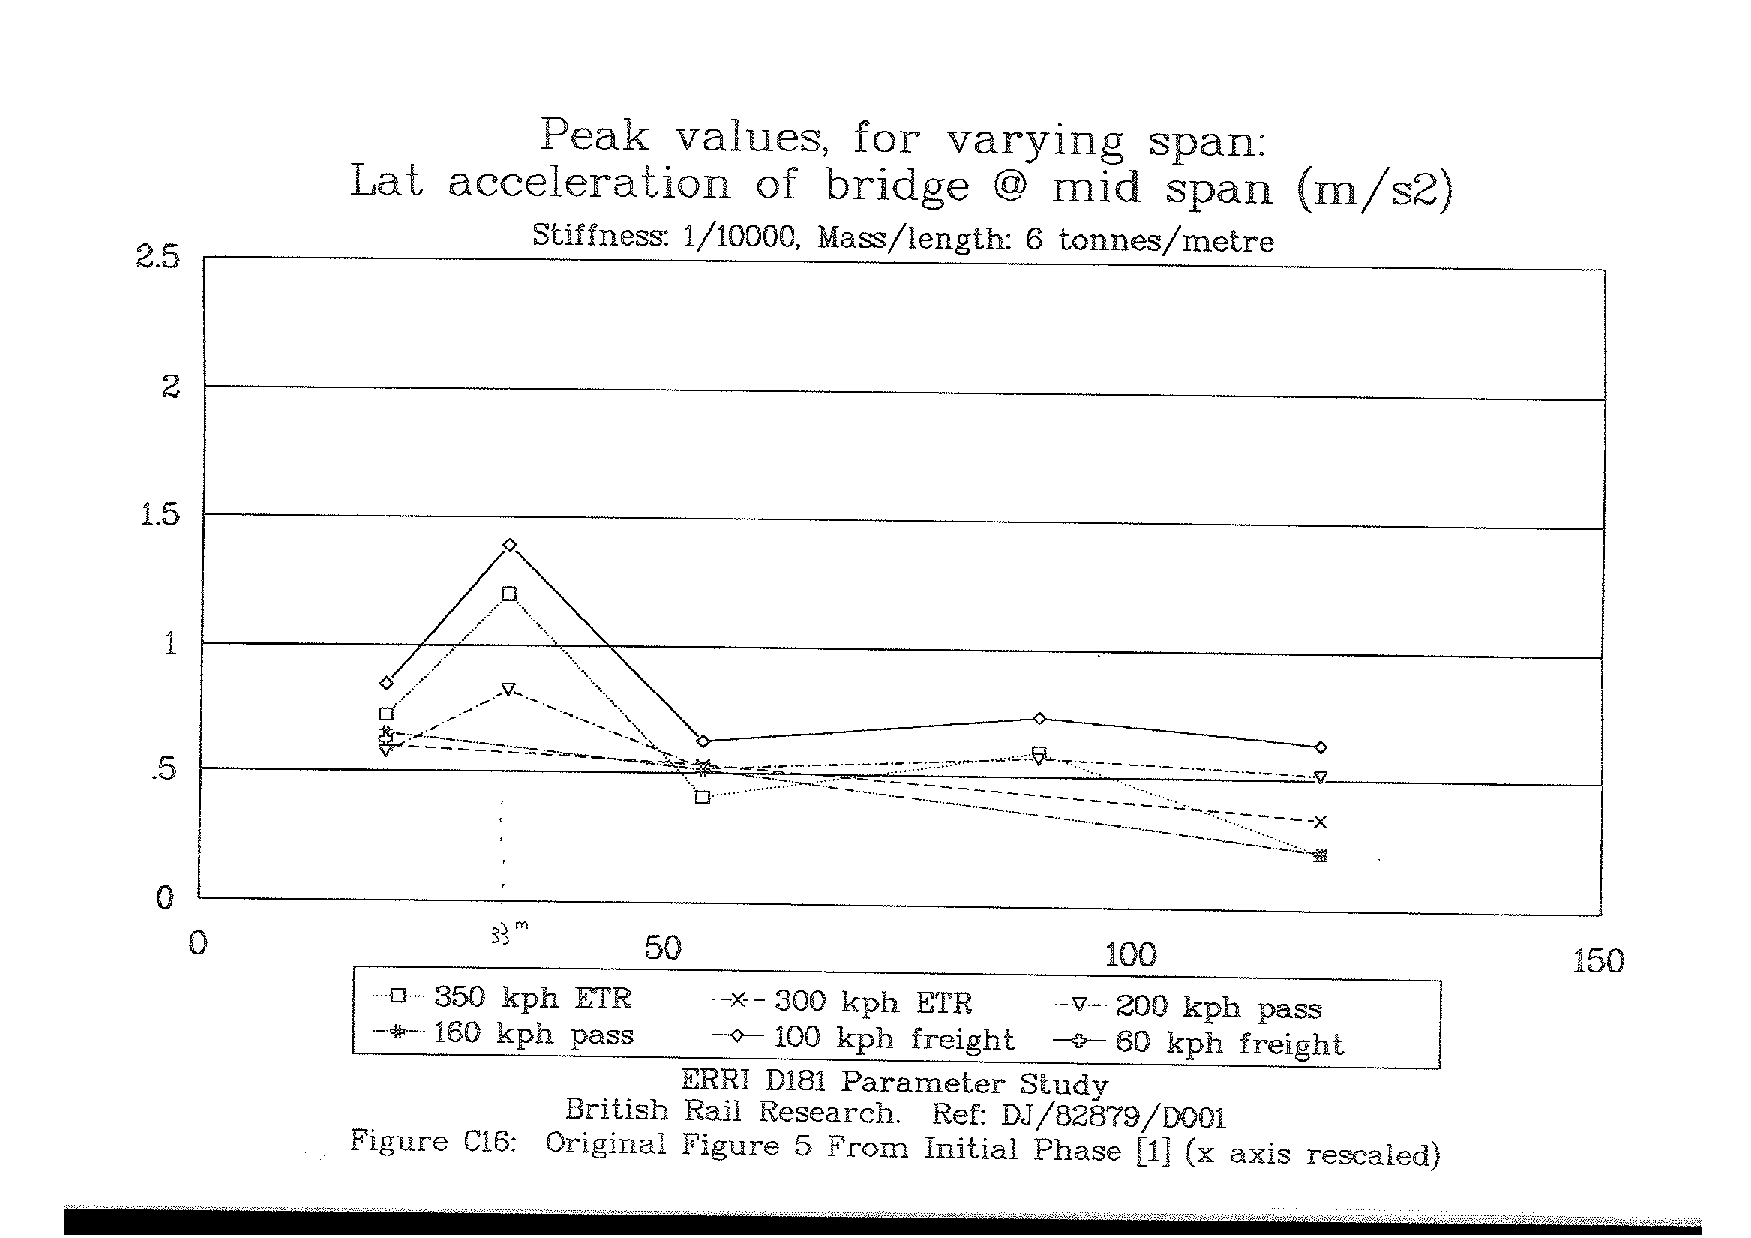
\includegraphics[width=0.8\textwidth]{c16.pdf}
%     \caption{Evidence of resonance caused by kinematic wavelength with span. Extract from \cite[C16]{d181dt329} }
%     \label{fig:c16}
% \end{figure}

% Although wavelength coincidence with span resonance is possible, for longer span bridges (span larger than 50m) it's hardly possible for this type of resonance to build up because the span of the bridge is greater than the wavelength of the train. However, resonance caused by kinematic frequency coincidence with first bending mode is possible even if wavelength and span doesn't match.

% In this report, emphasis is placed on long span bridges, thus resonance cause by kinematic wavelength with span is not investigated due to above reasons. On the other hand, frequencies of kinematic movements of trains will be studied. 

% \section{Conclusion}
% As discussed in Section.\ref{sec:1.2hz} that the origin of natural frequency remains unknown, it is highly doubted that it's actually the frequency range of vehicle suspension system. Rough calculations have been done to study the natural frequencies of the suspension systems of train examples provided in DT 329, proofing all of the frequencies calculated are within a range of 0.3Hz to 1.0Hz. This result mostly overlaps with the frequency range provided by 1.2Hz criterion proposal. 

% If this hypothesis is true, it can also be concluded that D181 committee made a serious mistake in their criterion proposing. Dynamics of the suspension system is only a factor that influence the global dynamic behaviour of a running train, so as track irregularities, train speeds, train layouts, etc. Proposing a criterion based only on natural frequencies of the suspension system is unacceptable. What's more, CEN committee using this proposed criterion in Eurocode 1991-2 was another unconscious mistake.


% \chapter{Train vehicles layouts and geometry}



% \section{Locomotives}
% \subsection{4-axle locomotives}
% Generally, the relevant parameters for categorisation of 4-axle locomotives are axle load P (18 t to 22,5 t) and the bogie axle spacing (2,2 m to 3,4 m).

% Typically the mass per unit length is less than 6,4 t/m and the distance from the end axle to the end of the nearest coupling plane is greater than 1,9 m

% \subsection{6-axle locomotives}

% Generally, the relevant parameters for categorisation of 6-axle locomotives are:

% \begin{enumerate}[-]
% \item the maximum axle load P (18 t to 22 t) in combination with;
% \item the distance between axles within a bogie (1,80 m to 2,25 m).
% \end{enumerate}

% Typically, the mass per unit length (p) is less than 6,4 t/m and the distance from end axle to the end of the nearest coupling plane (a) is greater than 2,1 m.

% \section{Passenger carriages}
 
% \section{Wheelset and track dimensions}

% Generally the track guage is used as a distance measured between the two rails, more specifically the distance between the inside of the railheads measured 14mm below the surface of the rail. By choosing 14 mm the measurement is less influenced by lipping or lateral wear on the rail head and by the radius r = 13 mm of the rail head face. On normal track the gauge is $1435^{+10}_{-3}$ mm with with a maximum gradient of 1:3000. For new track, however, NS apply the following standards:

% \begin{enumerate}
% \item Mean gauge per 200 m: $1435^{+10}_{-1}$ mm
% \item Standard deviation within a 200 m section less than 1 mm
% \end{enumerate}

% \begin{figure}[h]
% \centering
% 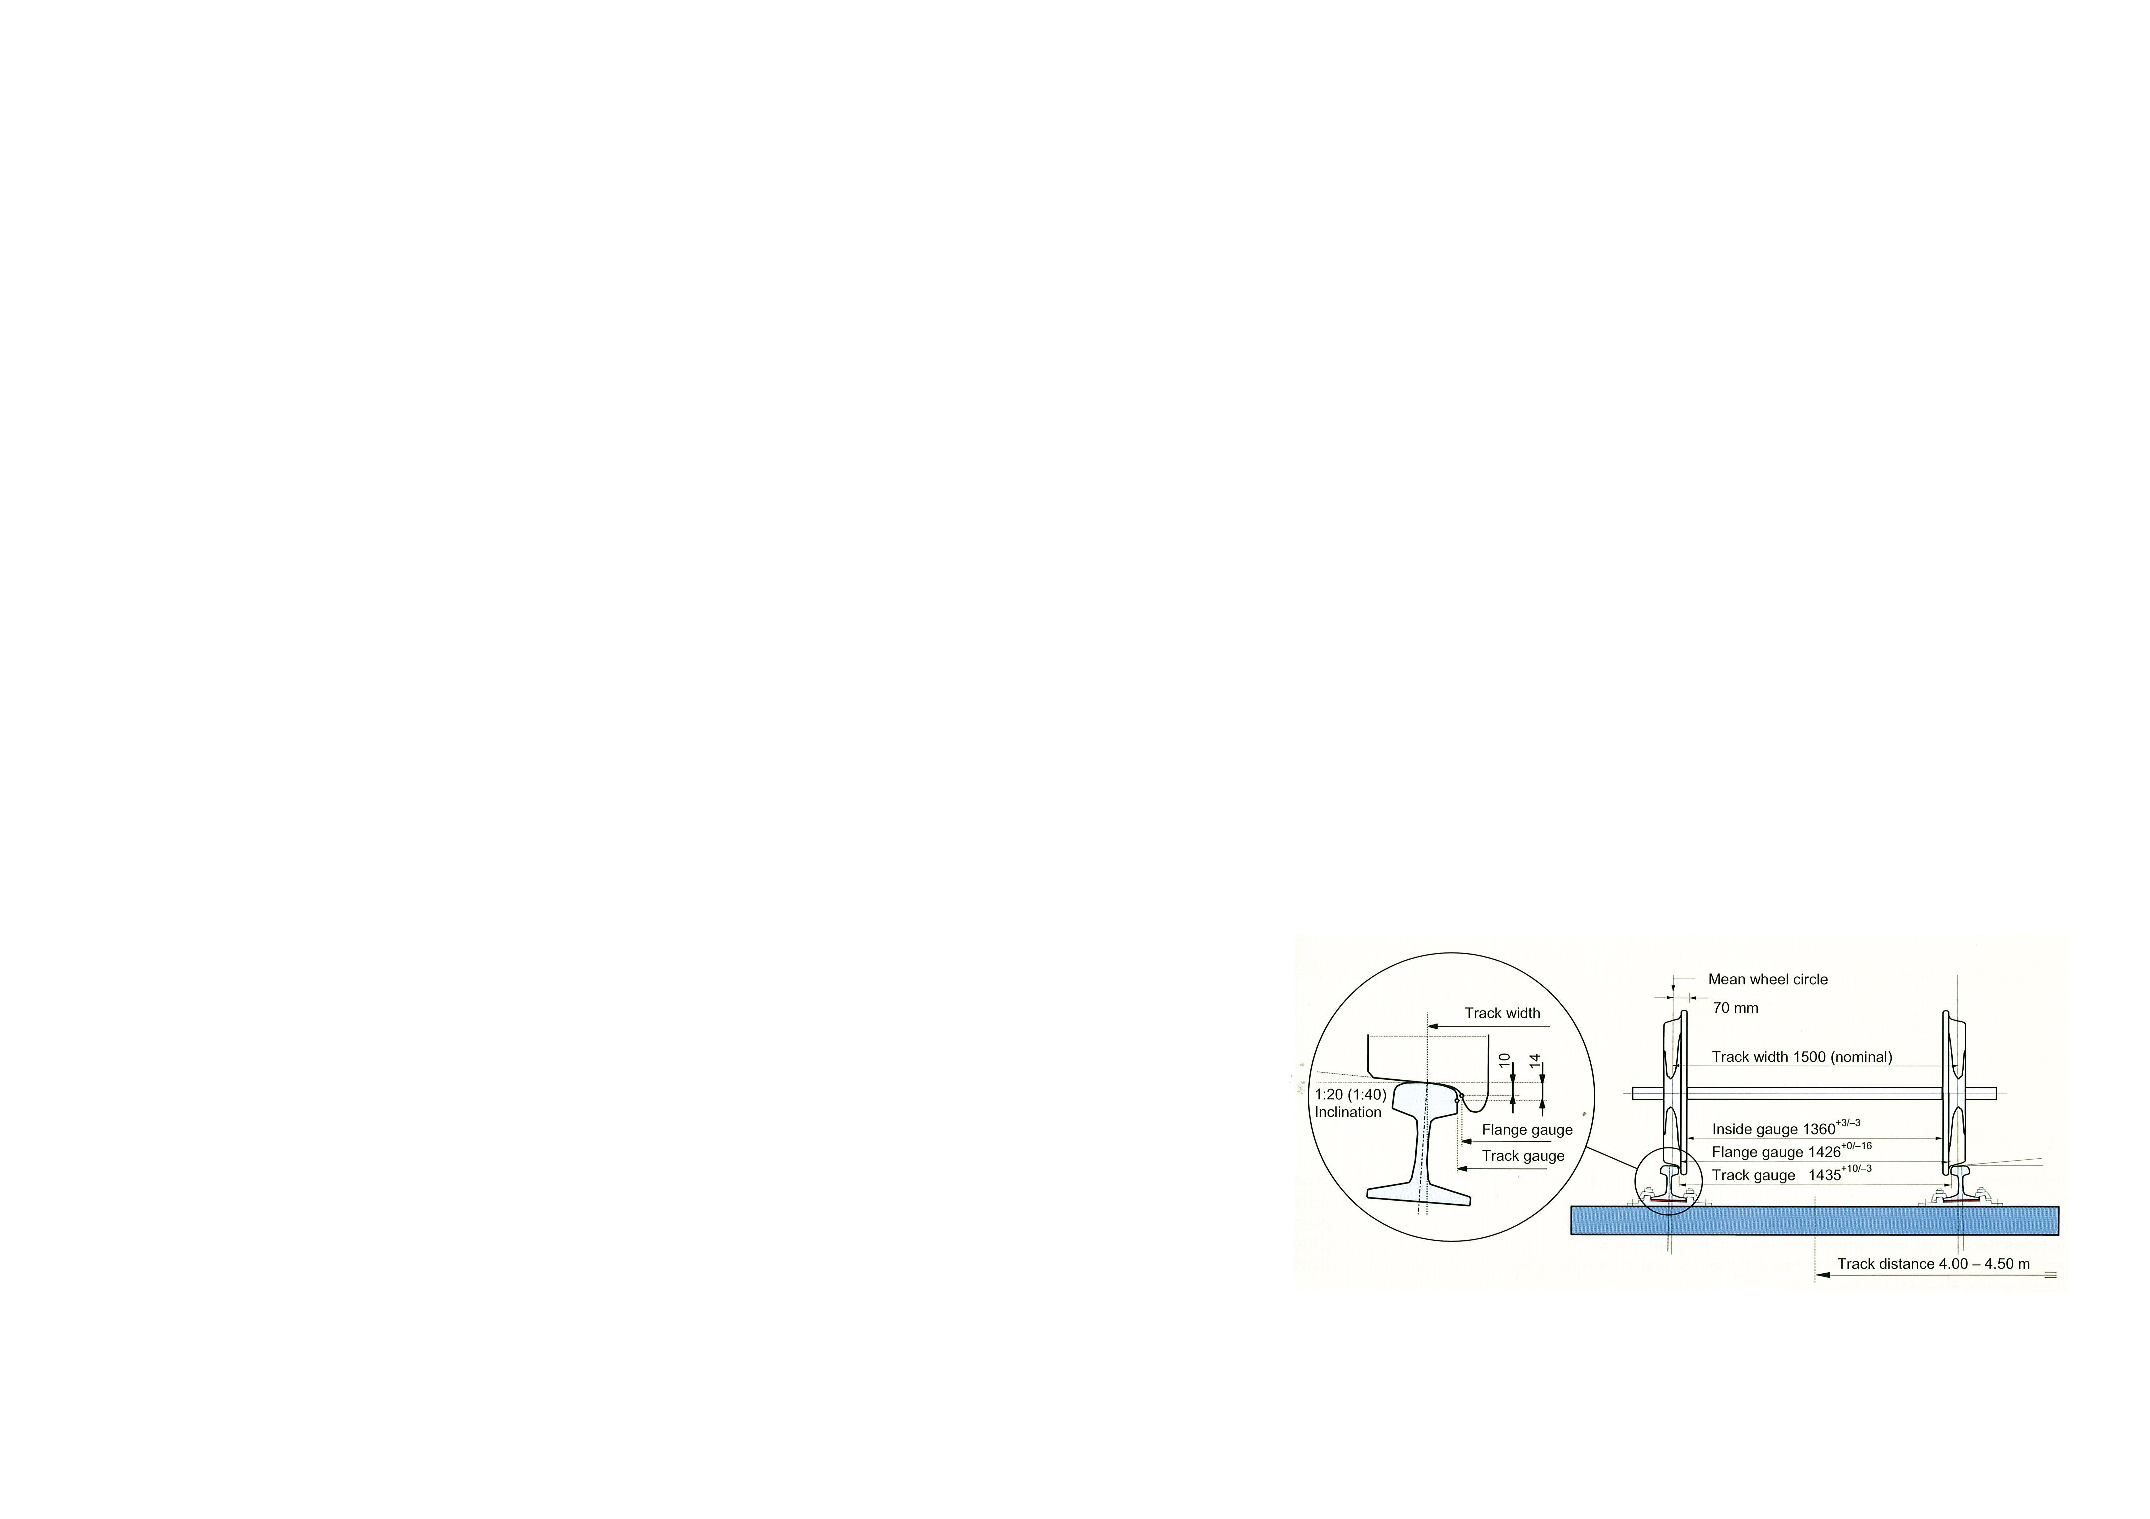
\includegraphics[width=0.8\textwidth]{wheelsettrackdimension.pdf}
% \caption{Wheelset and track dimensions for straight normal gauge track. Extracted from \cite[p.17]{esveld2001modern}}
% \label{fig:wheelset and track dimensions}
% \end{figure}


% \section{Conicity and Equivalent Conicity of Wheels}

% Originally conical tire profiles with an inclination of 1:20 were used. Since a centrally applied load on the railhead is desired, a rail inclination of 1:20, as shown in Figure 2.1, was also selected; this for instance still applies to NS profile NP 46. UIC 54 rail usually has an inclination of 1:40. This inclination matches the S 1002 worn wheel profile which is in general use in Europe. During manufacturing the tires are given a profile which matches the average shape cause by wear. In contrast to the straight conical profile this has a hollow form.

% It is clear that regarding a worn profile the conicity depends on the actual shape of the rail head and tire, including any wear, track gauge, and rail inclination. Likewise, elastic deformation of the wheelset and rail fastenings plays a role.

% Generally, the effective or equivalent conicity is defined as:

% $$ \gamma_e = \frac{\Delta r}{2y} = \frac{r_1 - r_2}{2y}  $$

% Here $r_1 - r_2$ is the instantaneous difference in rolling radius of the wheel treads; generally speaking this is a non-linear function of the lateral displacement y of the wheelset with respect to the central position. The difference between conical and worn profiles is given in Figure.\ref{fig:conicalwornprofiles}. To enable numerical comparisons $\gamma_e$ is determined at a certain lateral displacement $y=\bar{y}$.


% \begin{figure}[h]
%     \centering
%     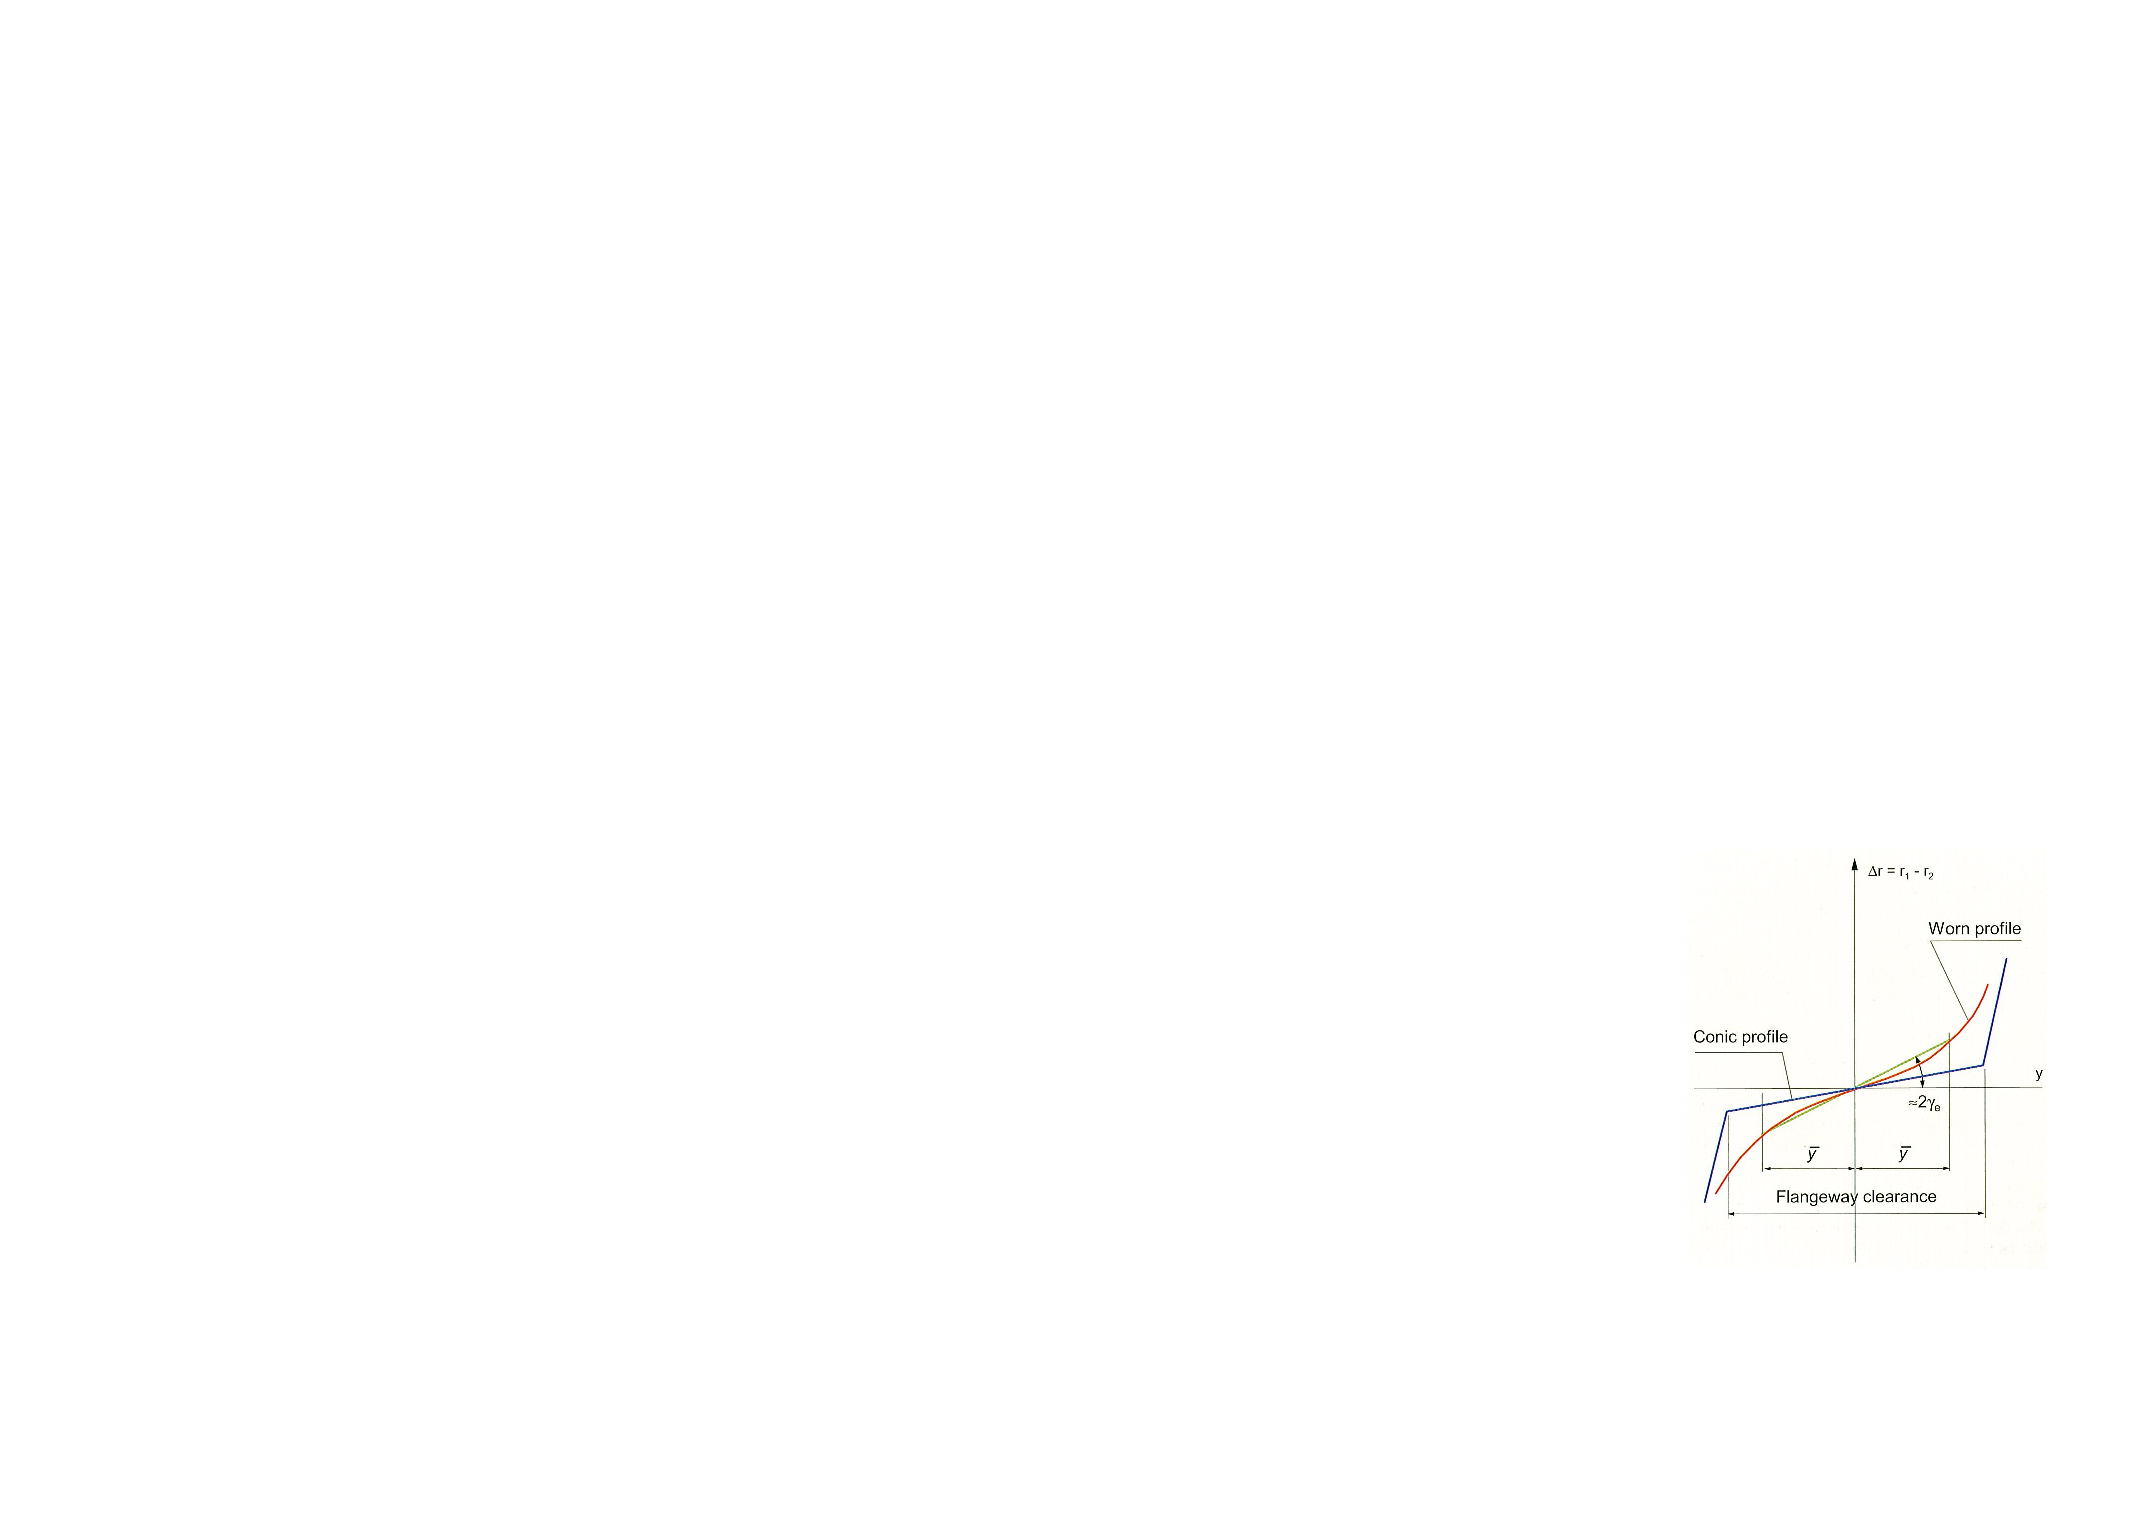
\includegraphics[width=0.6\textwidth]{conicalwornprofiles.pdf}
%     \caption{$y-\Delta r$ curves. Difference between conical and worn wheel profiles. Extracted from \cite[2.4]{esveld2001modern}}
%     \label{fig:conicalwornprofiles}
% \end{figure}

% With a conical profile the conicity is constant and above equation becomes:

% $$ \gamma_e = \frac{\Delta r}{2y} =\frac{(r+\gamma y)-(r-\gamma y)}{2y} = \gamma $$


% \section{Worn wheel profiles}

% A perfectly conical wheel profile is unstable as far as its shape is concerned, but will take on a shape that is stable as the effect of wear.

% Practical research has shown that over a period of time wheel profiles stabilise with wear at an equivalent conicity of 0.2 to 0.3. With regards to running stability, the equivalent conicity must remain below 0.4 and to ensure the centering effect it must be greater than 0.1.

% \section{Trains in Netherlands}

% Passenger trains now in service include following models:

% \begin{enumerate}
%     \item The DD-AR (Dubbeldeksaggloregiomaterieel) \\  EMUs were delivered as DDM-2/3 resembling the bilevel rail cars series DDM-1 from 1985 and operates in fixed formations of 3 or 4 coaches. 4 car trains use a class 1700 locomotive for traction, 3 car trains use an mDDM motorcar, which resembles a DD-AR driving trailer but has electric motors and a single passenger deck on top; the level of this deck is higher than that of a regular single deck rail car, but lower than the upper deck of the other coaches. Three types of coaches are available: Bv (second class), ABv (first and second class) and Bvk (second class driving trailer). The DDM-2/3 series are being modernised from 2010–2013 and after modernisation the series was renamed as NID (Nieuwe Intercity Dubbeldekker).
%     \item The VIRM (Verlengd Interregiomaterieel) \\ also called Regiorunner was partially rebuilt from trainsets DD-IRM (Dubbeldeks Interregiomaterieel). DD-IRM was delivered in 3- and 4-car trainsets. 3-car trainsets got one extra coach, 4-car trainsets got two extra coaches. Also, new 4- and 6-car trainsets were built. Thus, a train consists of one or more combinations of 4 or 6 double deck coaches; each combination (multiple unit) has electric motors. More than three hundred coaches are currently operative in the Netherlands.
%     \item The Koploper (ICM) (Intercitymaterieel) \\ is a 3- or 4-car multiple unit that when coupled with another one, allows passengers to walk through (the name Koploper being a play on words – literally "head walker", but in actual use meaning "front runner"). The Dutch Railway Company decided to close the heads permanently on 31 October 2005 because the mechanism broke down too often. A scheduled modernisation of around 7 million euro will see the ICM fleet updated. The renovated ICM trains provide 13\% more seats (reducing the leg room to uncomfortable small for the long haul journeys they serve in 2nd class, which is further aggravated by a waste bin that is placed on the backsides of the seats in front), have a new interior, a bathroom accessible by wheelchairs, airconditioning as well as upgrades to the engine and connection systems. The head doors are removed. Also, these (renovated) trains are the first trains in the NS fleet equipped with OBIS. OBIS provides a (free) WiFi-connection on board, along with in-train journey information provided through screens and (automated) vocal announcements through the trains speakers. This journey information provides the actual status, and thus is always up-to-date to the actual situation this trip, and the stations is passes.
%     \item The Sprinter (SGM, Stads Gewestelijk Materieel) \\ is a two or three car electric, used on small distances. They are named Sprinter because they're able to accelerate and brake quite fast, making them very suitable for 'stoptrein' services. They were also specifically designed for urban environments where they run commuter services. As a result, they are most commonly found in the Randstad area. The initial idea was that the Sprinter would provide somewhat of a subway/metro service but this plan failed as the cities of Amsterdam and Rotterdam continued to construct their own rapid transit systems. Nevertheless, in the densely populated Randstad, the Sprinters remain popular. Two car versions were revised and renamed to Citypendel. All Sprinters are now refurbished into the new white/yellow/dark blue livery.
% \end{enumerate}

% All of passenger train coaches have a wheel diameter of 920 mm. 

% Locomotives of freight trains have wheel diameter of 1000 mm.

% \section{Lateral Track Irregularities}
% This section describes allowable lateral track irregularities defined in EN13848-5\cite{13848}. 

% Lateral alignment irregularities was defined in EN13838-1. It states:"Deviation $y_p$ in y-direction of consecutive positions of point P... on any rail, expressed as an excursion from the mean horizontal position (reference line) covering the wavelength ranges stipulated below and calculated from successive measurements ...". See Figure \ref{fig:lateraldeviationdefine}.

% For lateral deviations, the following wavelengths shall be considered: $D1 = 3 -25 m$, $D2 = 25 - 70 m$ and $D3 = 70 - 200 m$. 

% \begin{figure}[h]
%     \centering
%     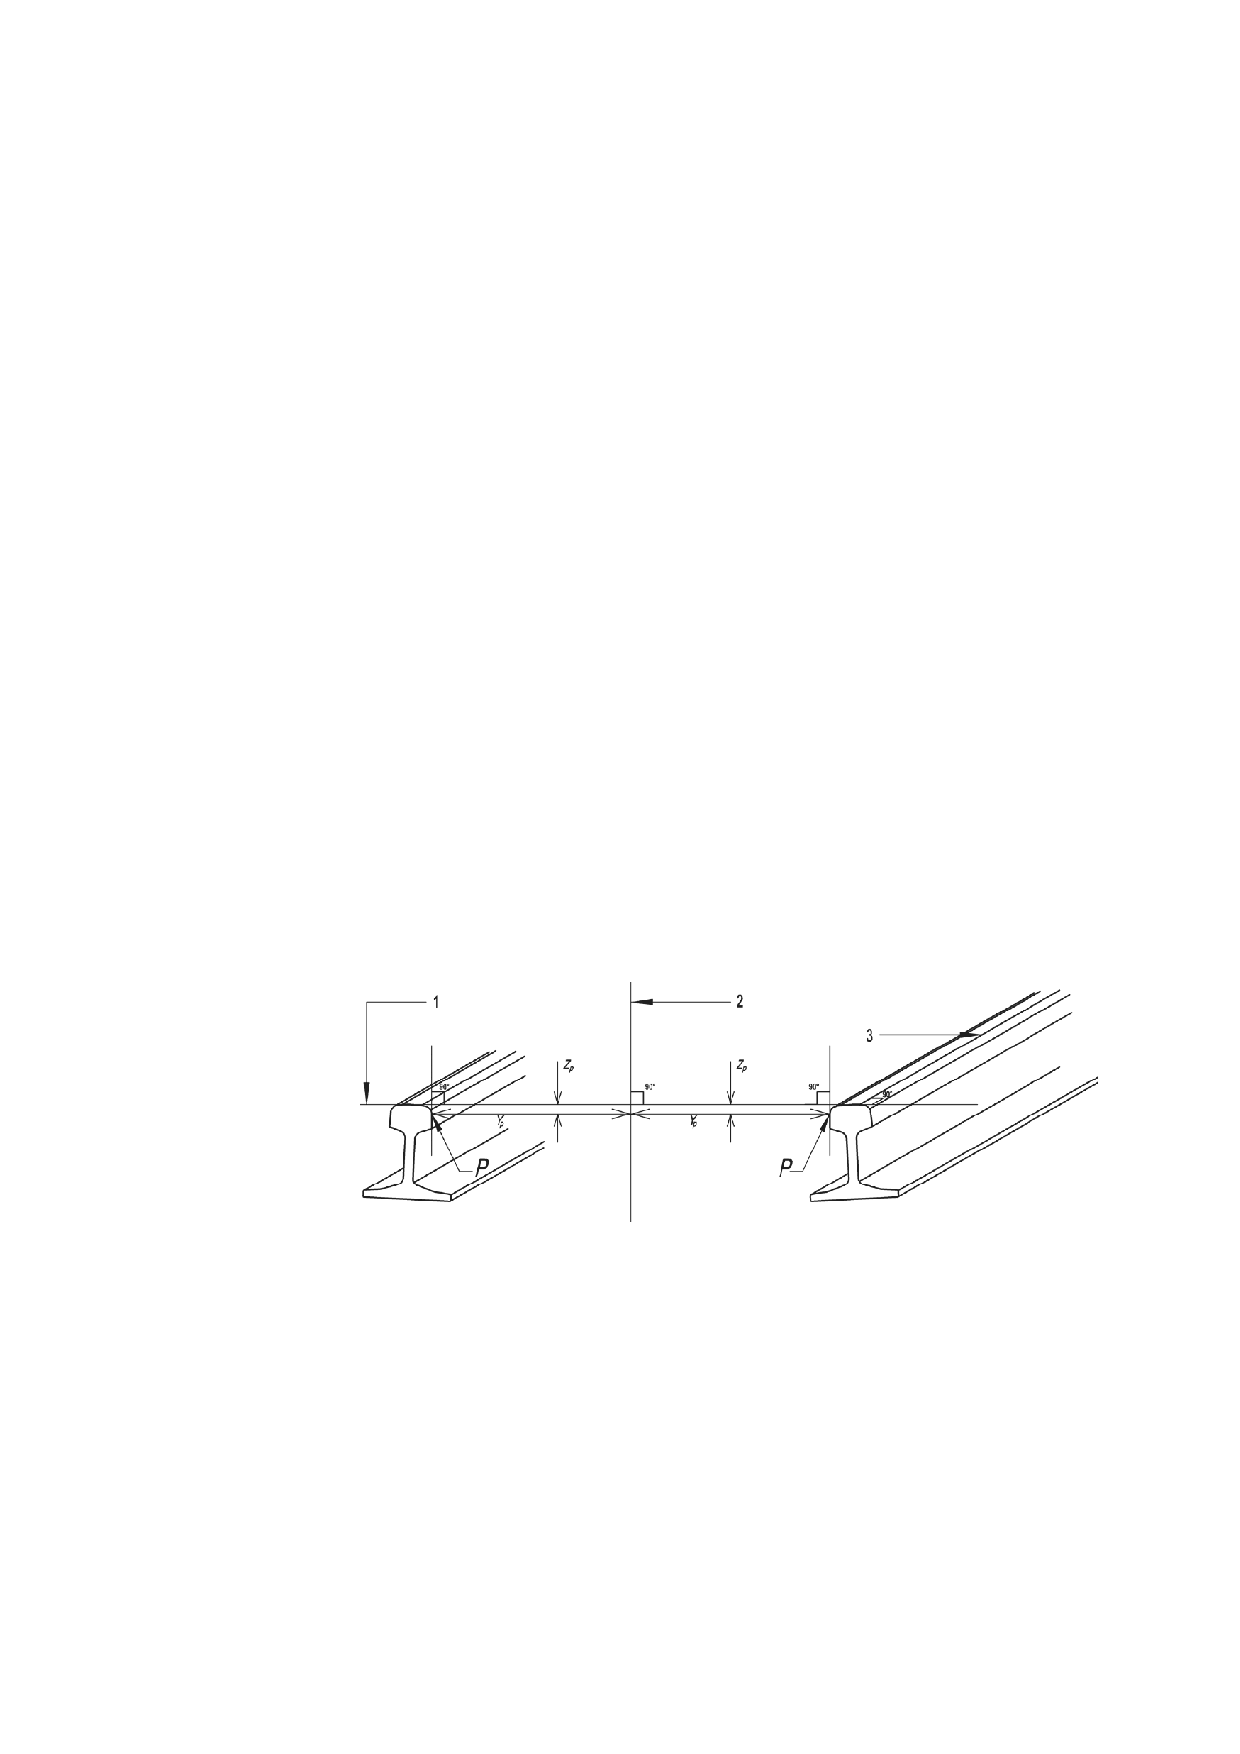
\includegraphics[width=0.8\textwidth]{lateraldeviationdefine}
%     \caption{Lateral deviation definition. Lateral deviations $y_p$ for each rail with 1: running surface, 2: reference line and 3: centre line of running table}
%     \label{fig:lateraldeviationdefine}
% \end{figure}

% Table \ref{tab:lateraldeviation} defines the allowable standard deviation for lateral track irregularities.

% \begin{table}[h]
%     \centering
%     \caption{Alignment - AL - Standard deviation. Extracted from \cite[Table B.6]{13848}}
%     \begin{tabular}{cc}
%         \hline
%         Speed(km/h) & Standard deviation(mm) \\
%         \hline
%         $V\leq 90$ & 1.5 to 1.8 \\
%         $80 < V \leq 120$ & 1.2 to 1.5 \\
%         $120 < V \leq 160$ & 1.0 to 1.3 \\
%         $160 <V \leq 230$ & 0.8 to 1.1 \\
%         $230 <V \leq 300$ & 0.7 to 1.0 \\
%         \hline
%     \end{tabular}
%     \label{tab:lateraldeviation}
% \end{table}


\chapter{Study on vehicle wavelength}
% The objective of parametric study is to observe lateral vibration frequency range of different trains types. Due to limited source of reliable vehicle data, train modelled in this study is the same train data used in ERRI Report RP6\cite{d181} where necessary. Considering effects that was assumed to have been taken into account by ERRI in previous chapter, following parameters to be checked are determined. 

% Parameters to be examined:
% \begin{enumerate}
% \item different layouts
% \item suspension system stiffness
% \item mass of the train
% \item track irregularities
% \item bridge span
% \item bridge mass
% \item bridge stiffness
% \end{enumerate}


% To assess the effects of different parameters on train lateral frequency, following parametric study using FEM software are conducted. Please note that by default, the loading of every single axle is 22.5t, according to the maximum allowable axle load defined in \cite{EC15528}

% The process will start from comparably easy models then develop them into more sophisticated ones. With the development of the models, effects will be added into account one by one. Details of modelling will be described in following sections.

% \section{Basic phenomenon modelling}
% Phenomenon to be modelled: kinetic movement. track irregularities impact. 
% The aim of modelling is to reproduce FEM analysis by VAMPIRE software done by ERRI D181 committee in 1996. 

% Complicated simulation of vehicle-structure system is broken done into more basic modules. The order of modelling is shown in Fig.\ref{fig:modellingsequence}. More sophisticated model develops basing on simpler ones to minimize the appearance of errors. 

% \begin{figure}[h]
%     \centering
%     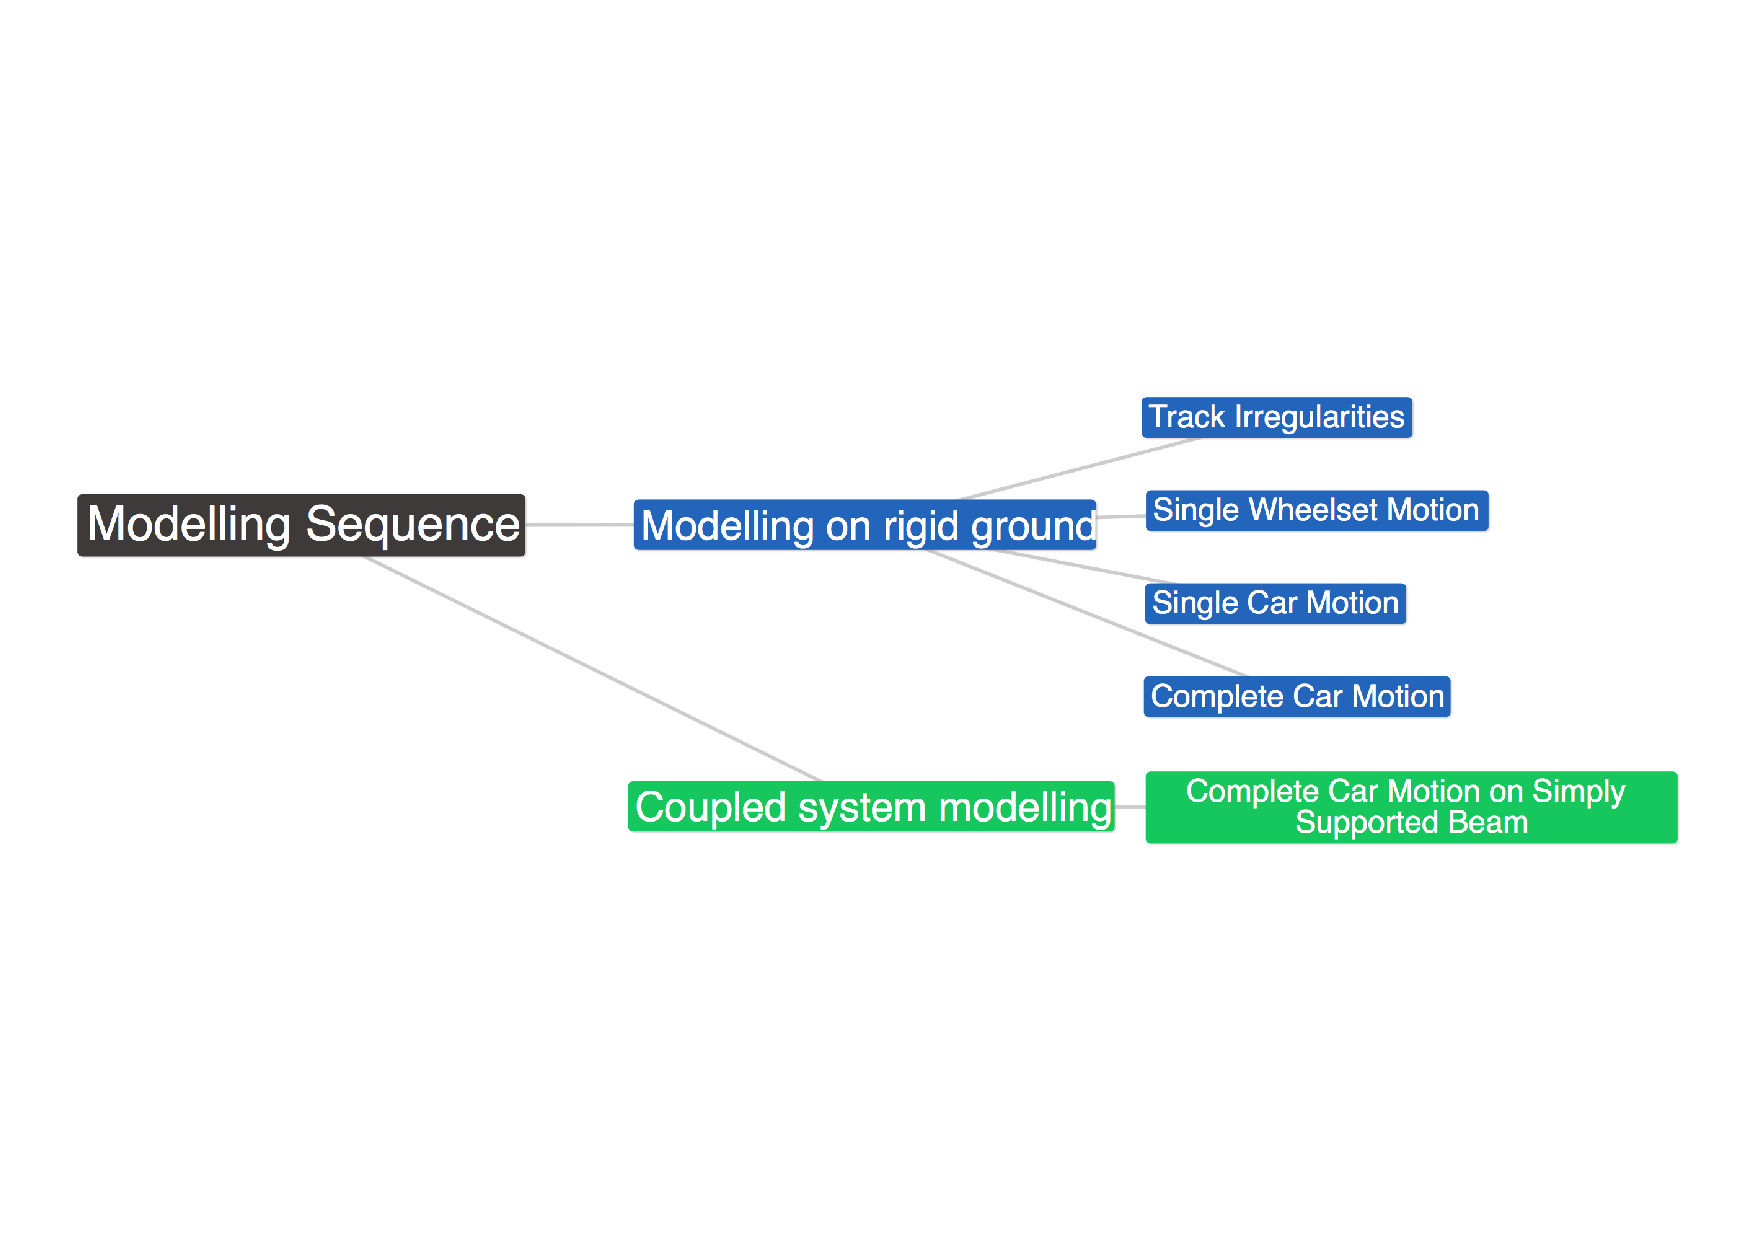
\includegraphics[width=0.8\textwidth]{modellingsequence.pdf}
%     \caption{Modelling sequence}
%     \label{fig:modellingsequence}
% \end{figure}


% \subsection{Track irregularities profile modelling}
% Trying to find a way of introducing track irregularities into the current model
% Track irregularities are small imperfections cause by manufacturing, train running, etc. Sample track irregularities over a certain length of track can be measured, as well as numerical generated. Track irregularities is the first effect to be modelled because it is the exciting source of other train lateral dynamic effects.

% An example of numerically generated track irrgularity profile is illustrated in Fig.\ref{fig:trackirregularities70_120}

% \begin{figure}[h]
%     \centering
%     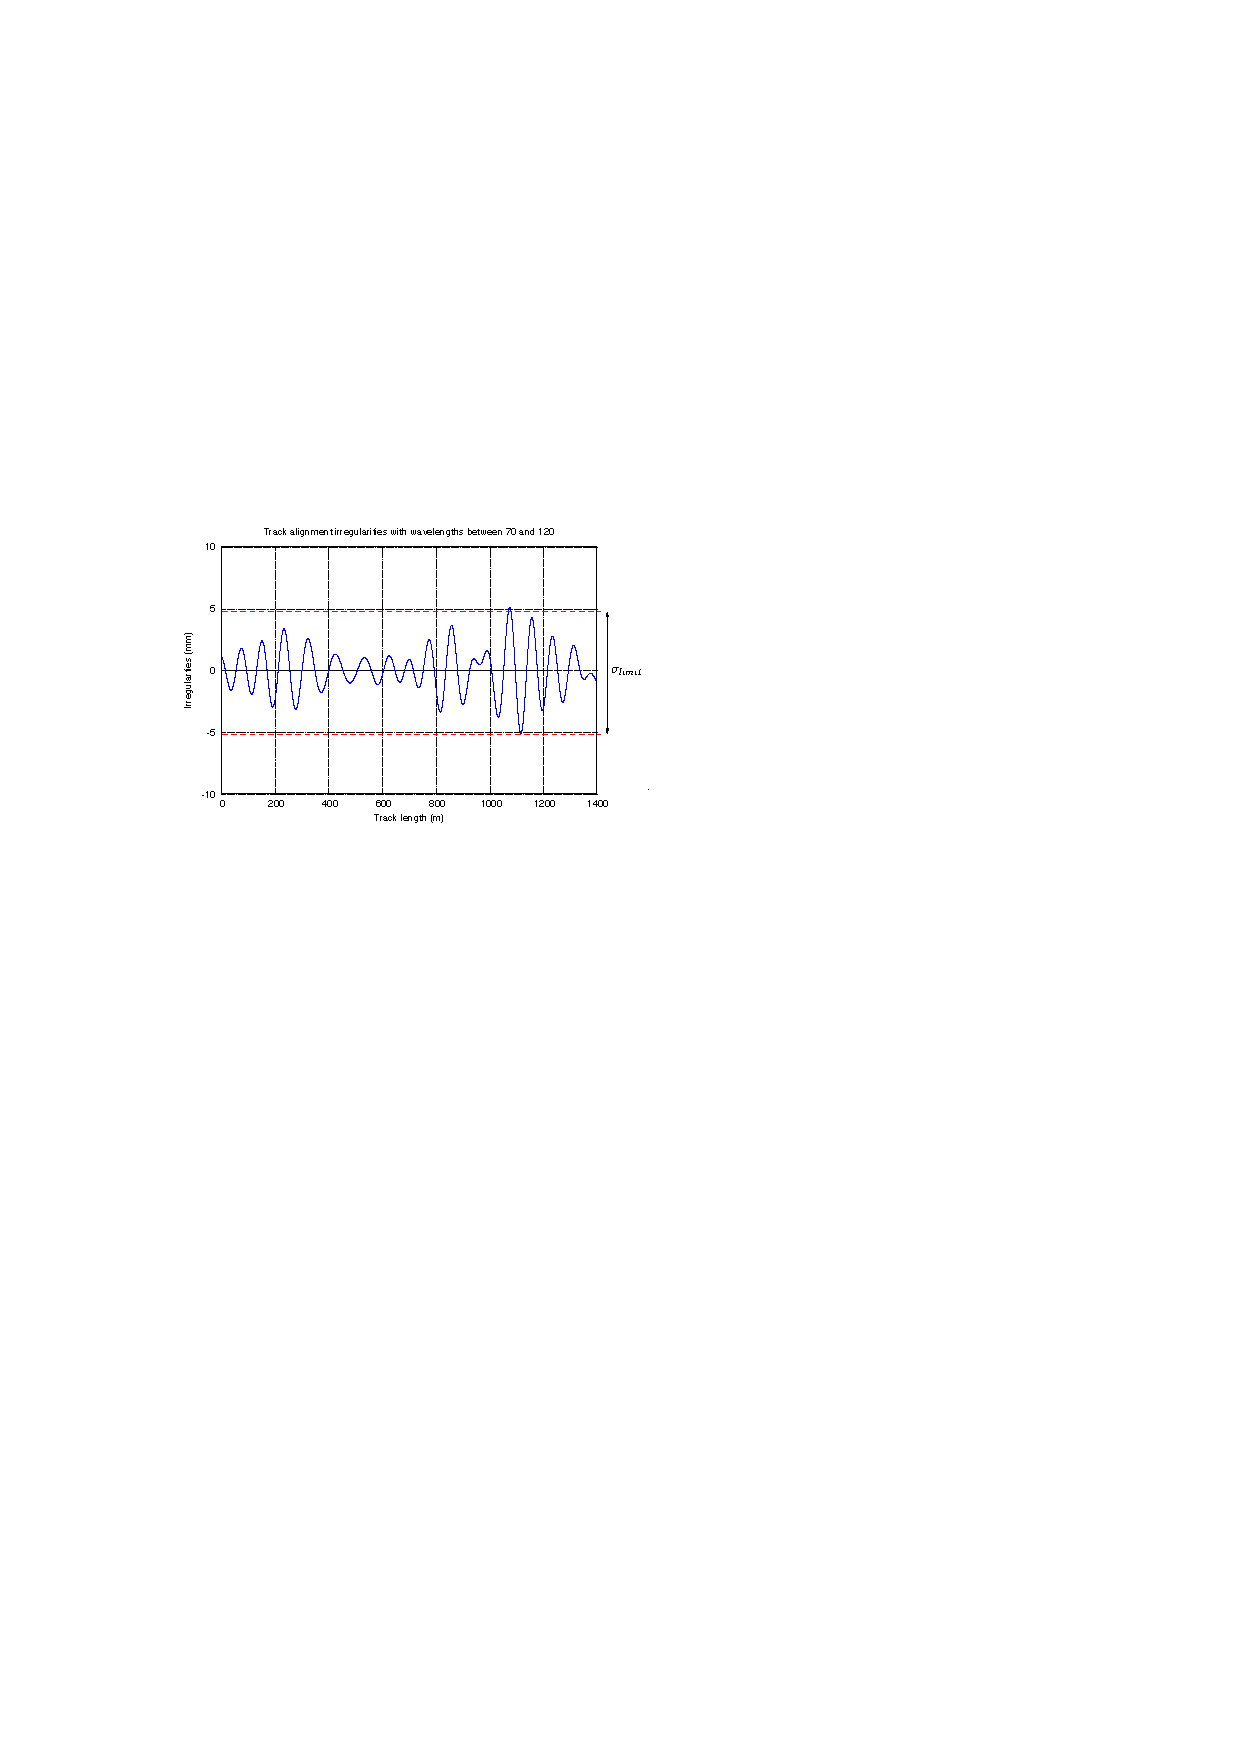
\includegraphics[width=0.8\textwidth]{trackirregularities70_120.pdf}
%     \caption{Track alignment irregularities with wavelengths between 70 and 120. Extracted from \cite{dias2008study}}
%     \label{fig:trackirregularities70_120}
% \end{figure}



% \subsection{Kinetic movement of single wheel-set}
% This step is to reproduce and evaluate the reliability of a basic wheelset-track model. The result of this model will be compared with Klingel formula.

% To be noted: Klignel kinematic movement description makes a number of simplifying assumptions since it neglects forces. For one, it assumes that the rolling resistance is zero. A wheelset (not attached to a train or truck), is given a push forward on a straight and level track. The wheelset starts coasting and never slows down since there are no forces (except downward forces on the wheelset to make it adhere to the track and not slip). But in the FEM model forces will be included to pave the way for following analyses.

% Research showed that Klingel's formula coincides well with measured data from experiments. This proves that if the result of this simulation coincides with what Klingel formula predicted, the model is reliable.

% This wheel-set will move on rigid and fixed tracks.

% Some thoughts:
% I need to model simplified contact stress, but due to unknown friction force, how do I maintain constant speed of train?

% \begin{figure}[h]
%     \centering
%     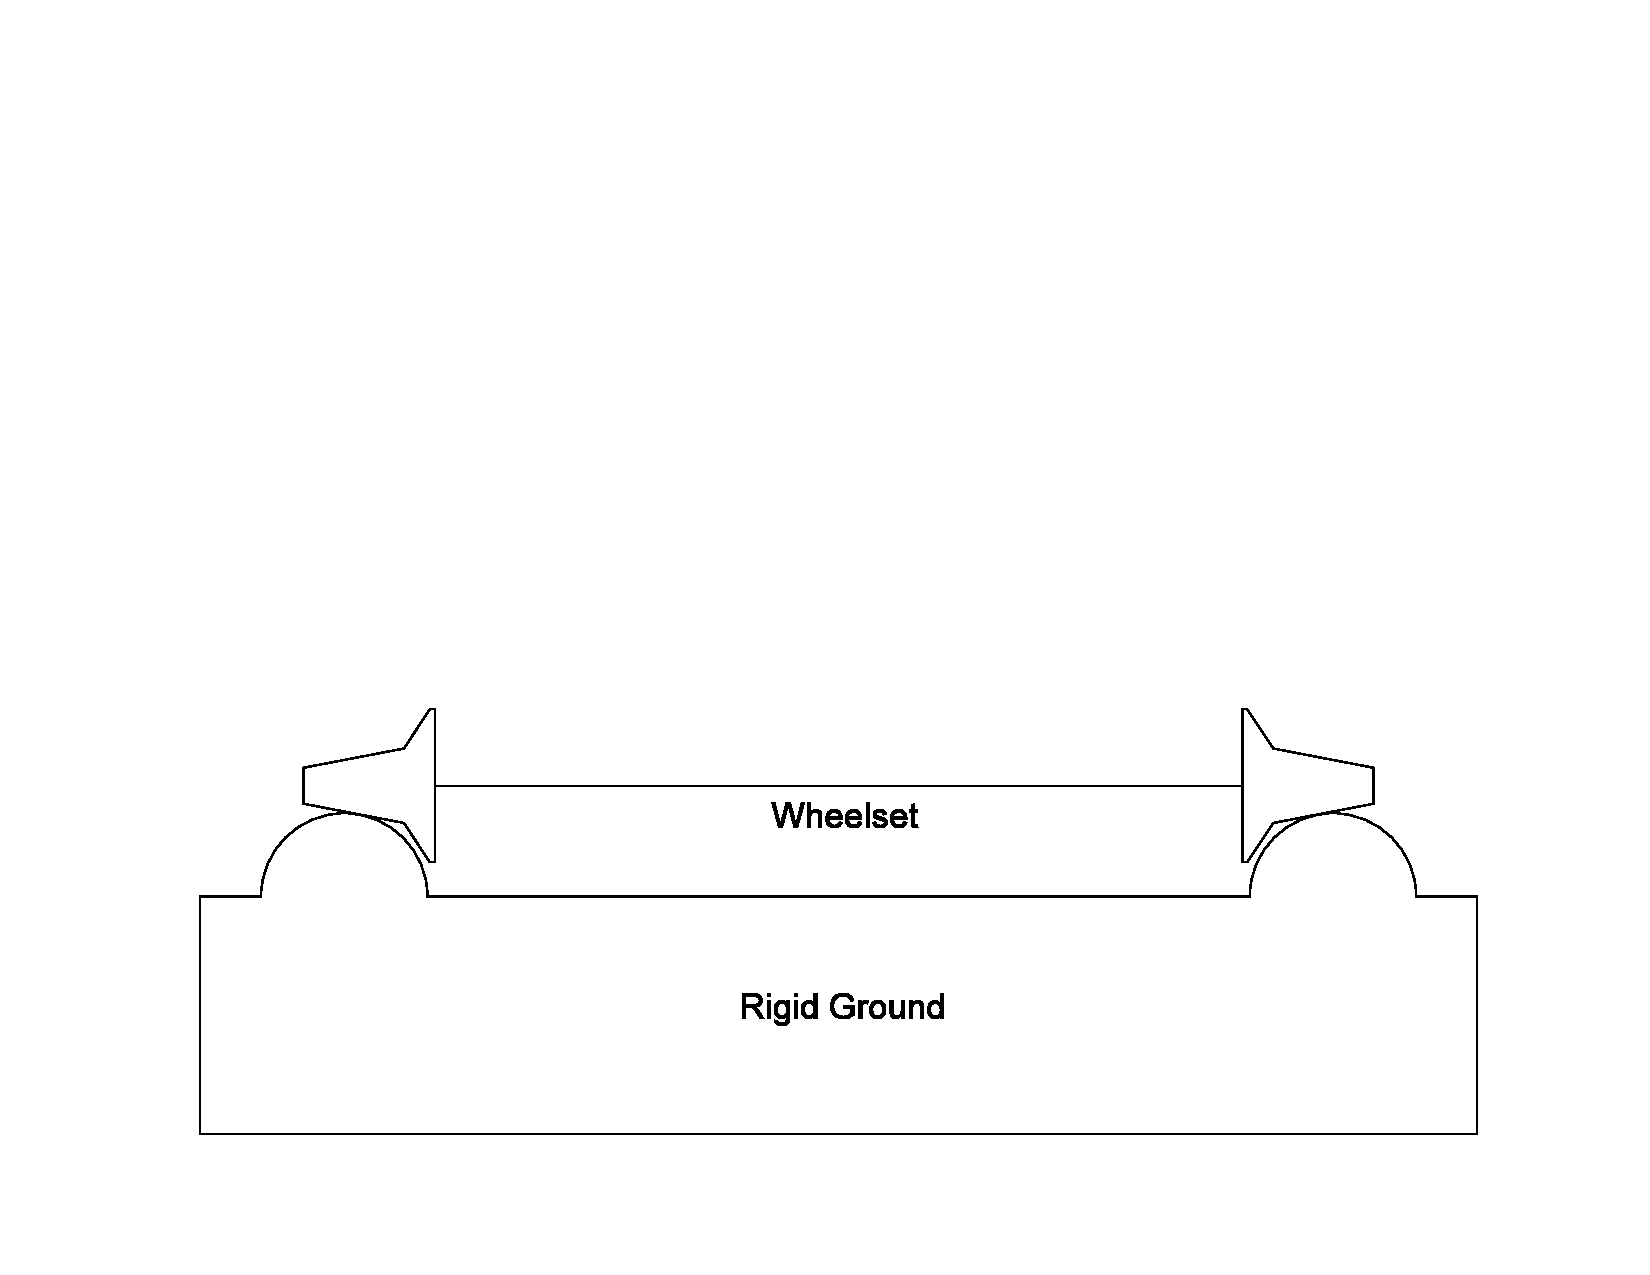
\includegraphics[width=0.5\textwidth]{wheelsetmodel.pdf}
%     \caption{Wheelset movement model}
%     \label{fig:wheelsetmovementmodel}
% \end{figure}

% \begin{figure}[h]
%     \centering
%     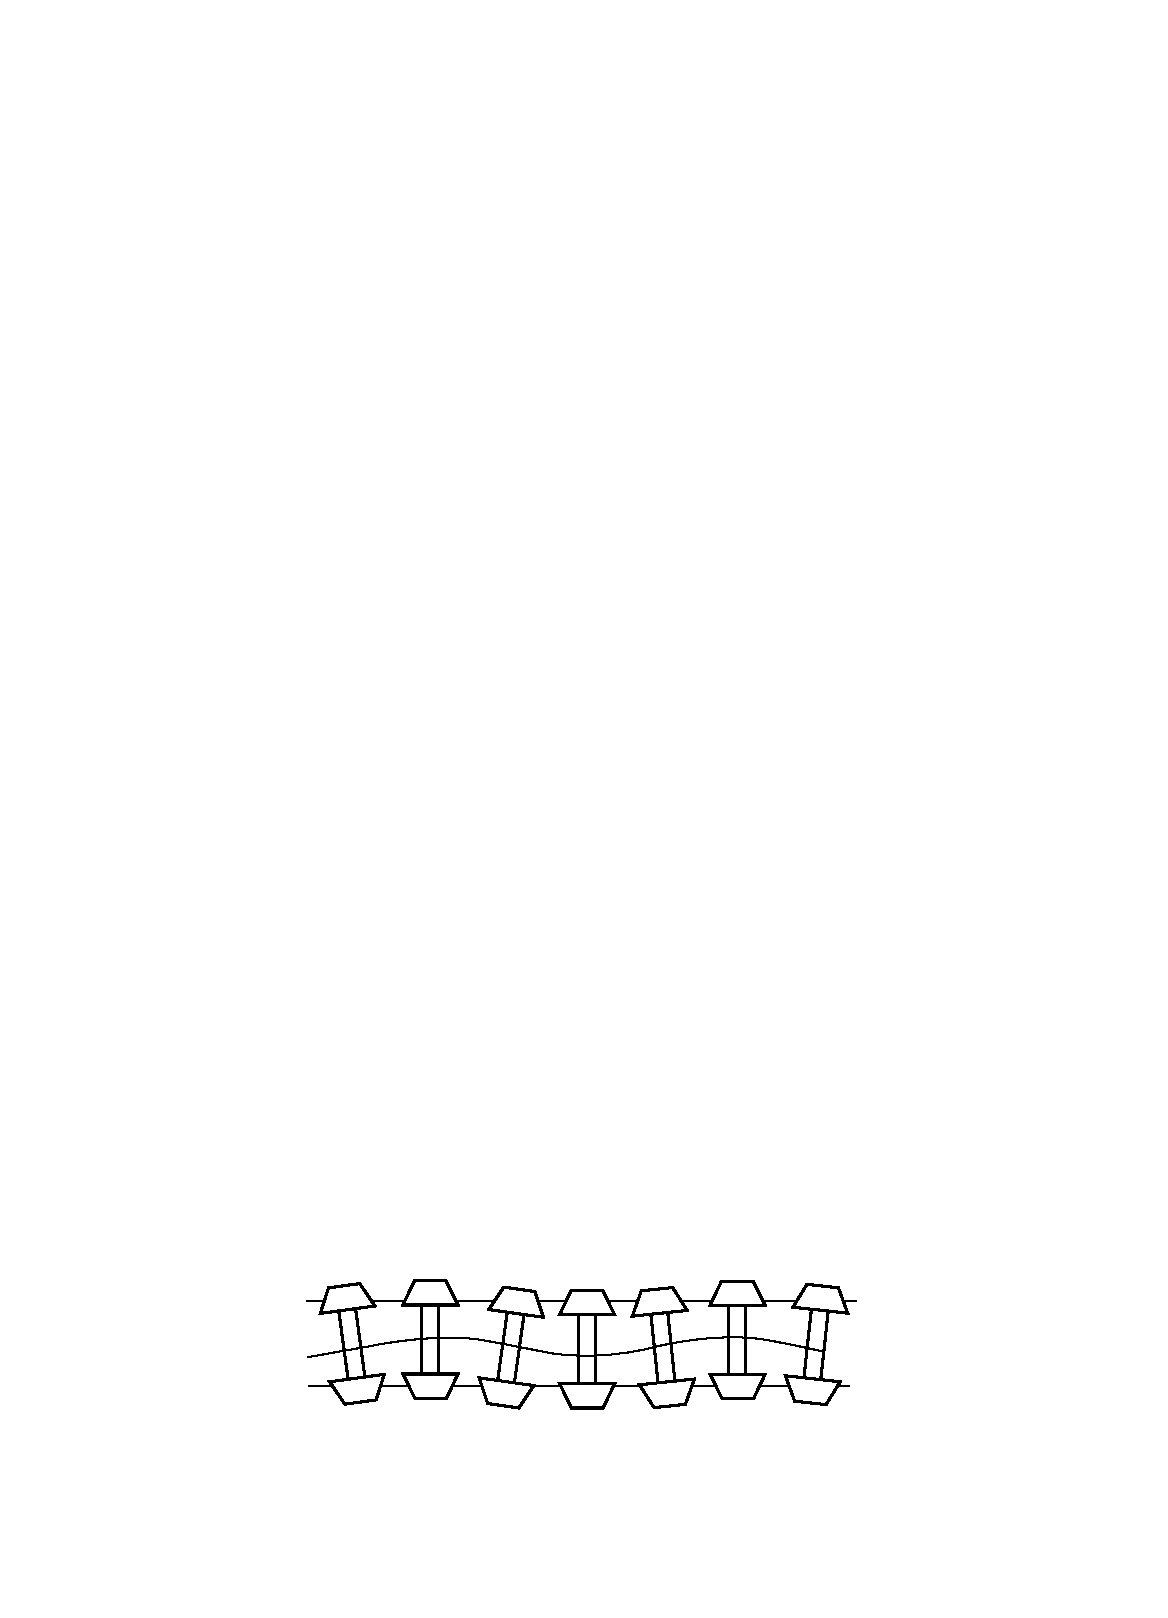
\includegraphics[width=0.8\textwidth]{singlewheelset.pdf}
%     \caption{Single wheel set kinetic oscillation view from top}
%     \label{fig:singlewheelset}
% \end{figure}


% \subsection{Kinetic movement of single car}
% This step is to add more sophisticated mass-spring system attached to the single wheel-set model in previous section. The mass-spring system represents the suspension system of cars in lateral direction. However, since the data to be used is the same data used in 1996, using more up-to-date train data is suggested for future researches.

% Several car types will be input including locomotives, passenger car and freight car.

% The car will move on flexible and fixed tracks. 

% \begin{figure}[h]
%     \centering
%     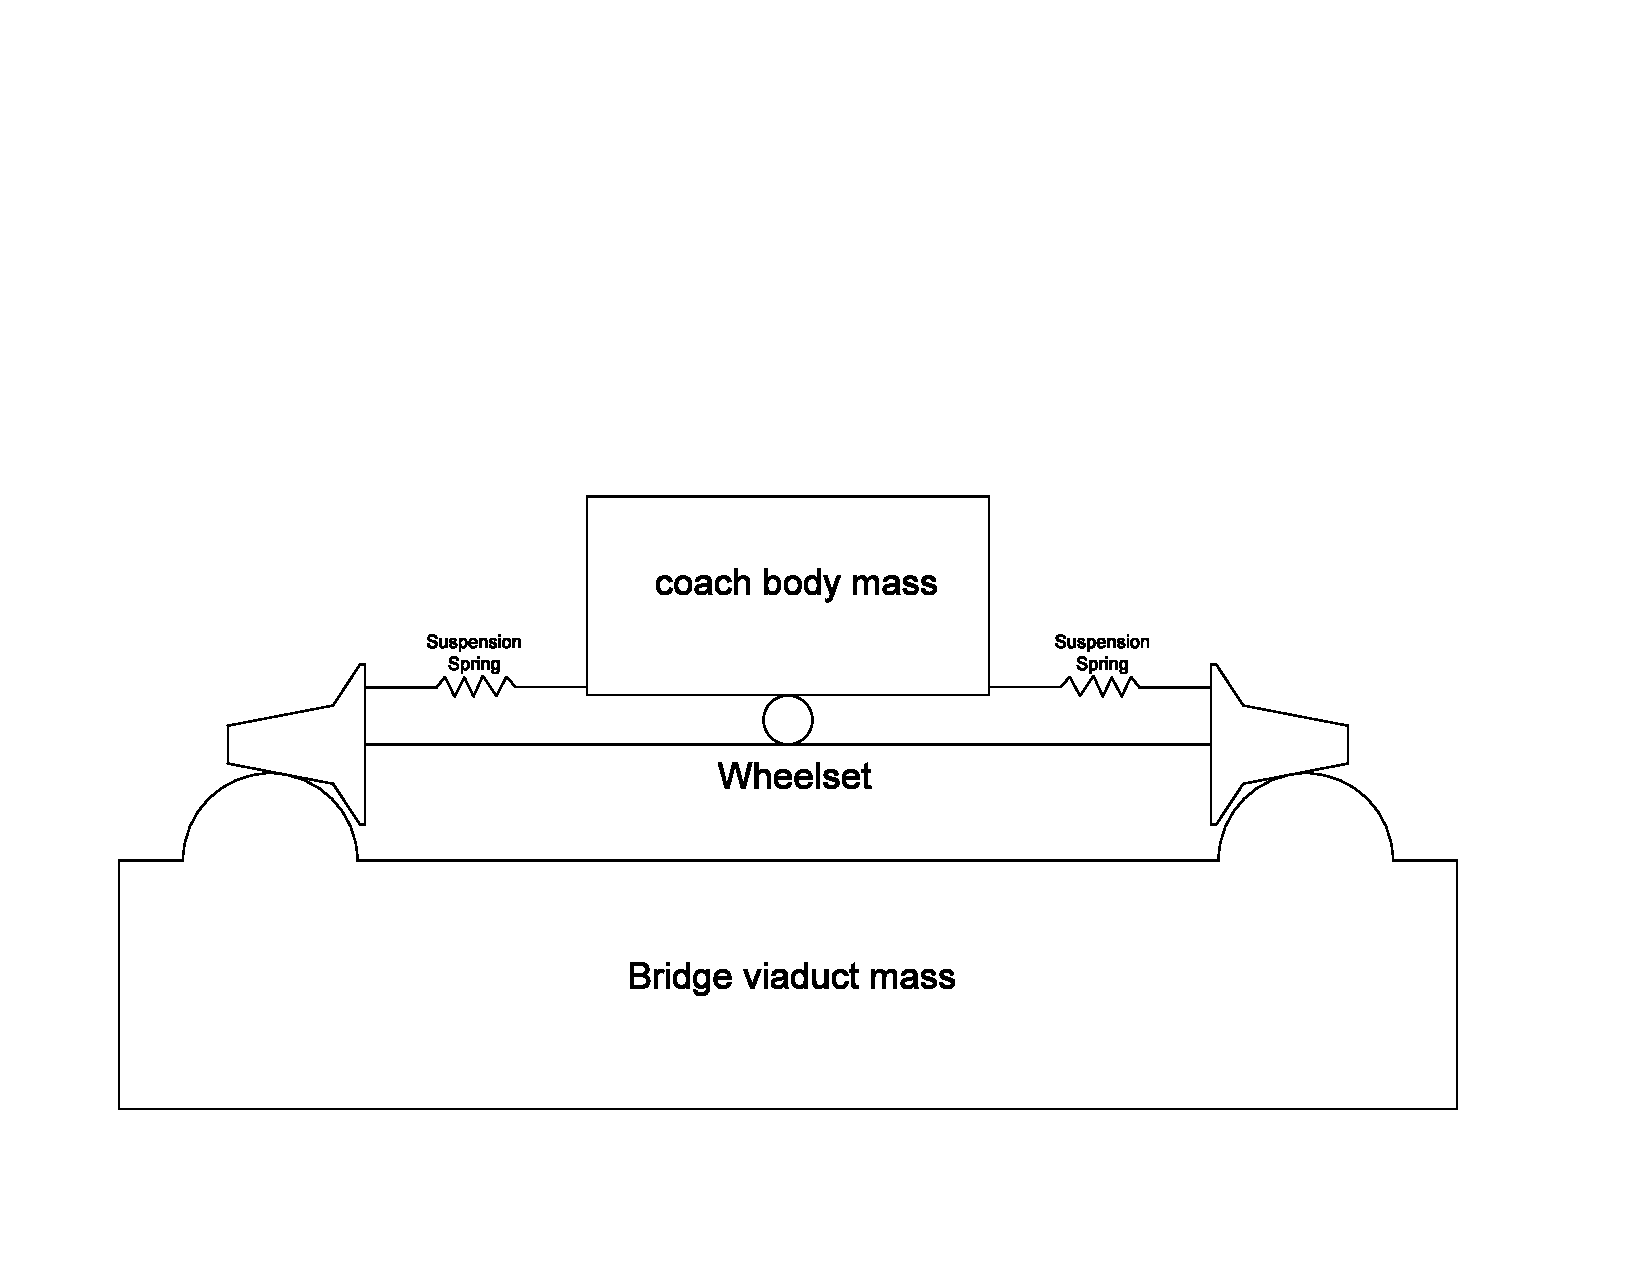
\includegraphics[width=0.5\textwidth]{trainmodellongwheelprofile.pdf}
%     \caption{Sample view of one single car model model used in FEM software from the front}
%     \label{fig:trainmodellong}
% \end{figure}

% \begin{figure}[h]
%     \centering
%     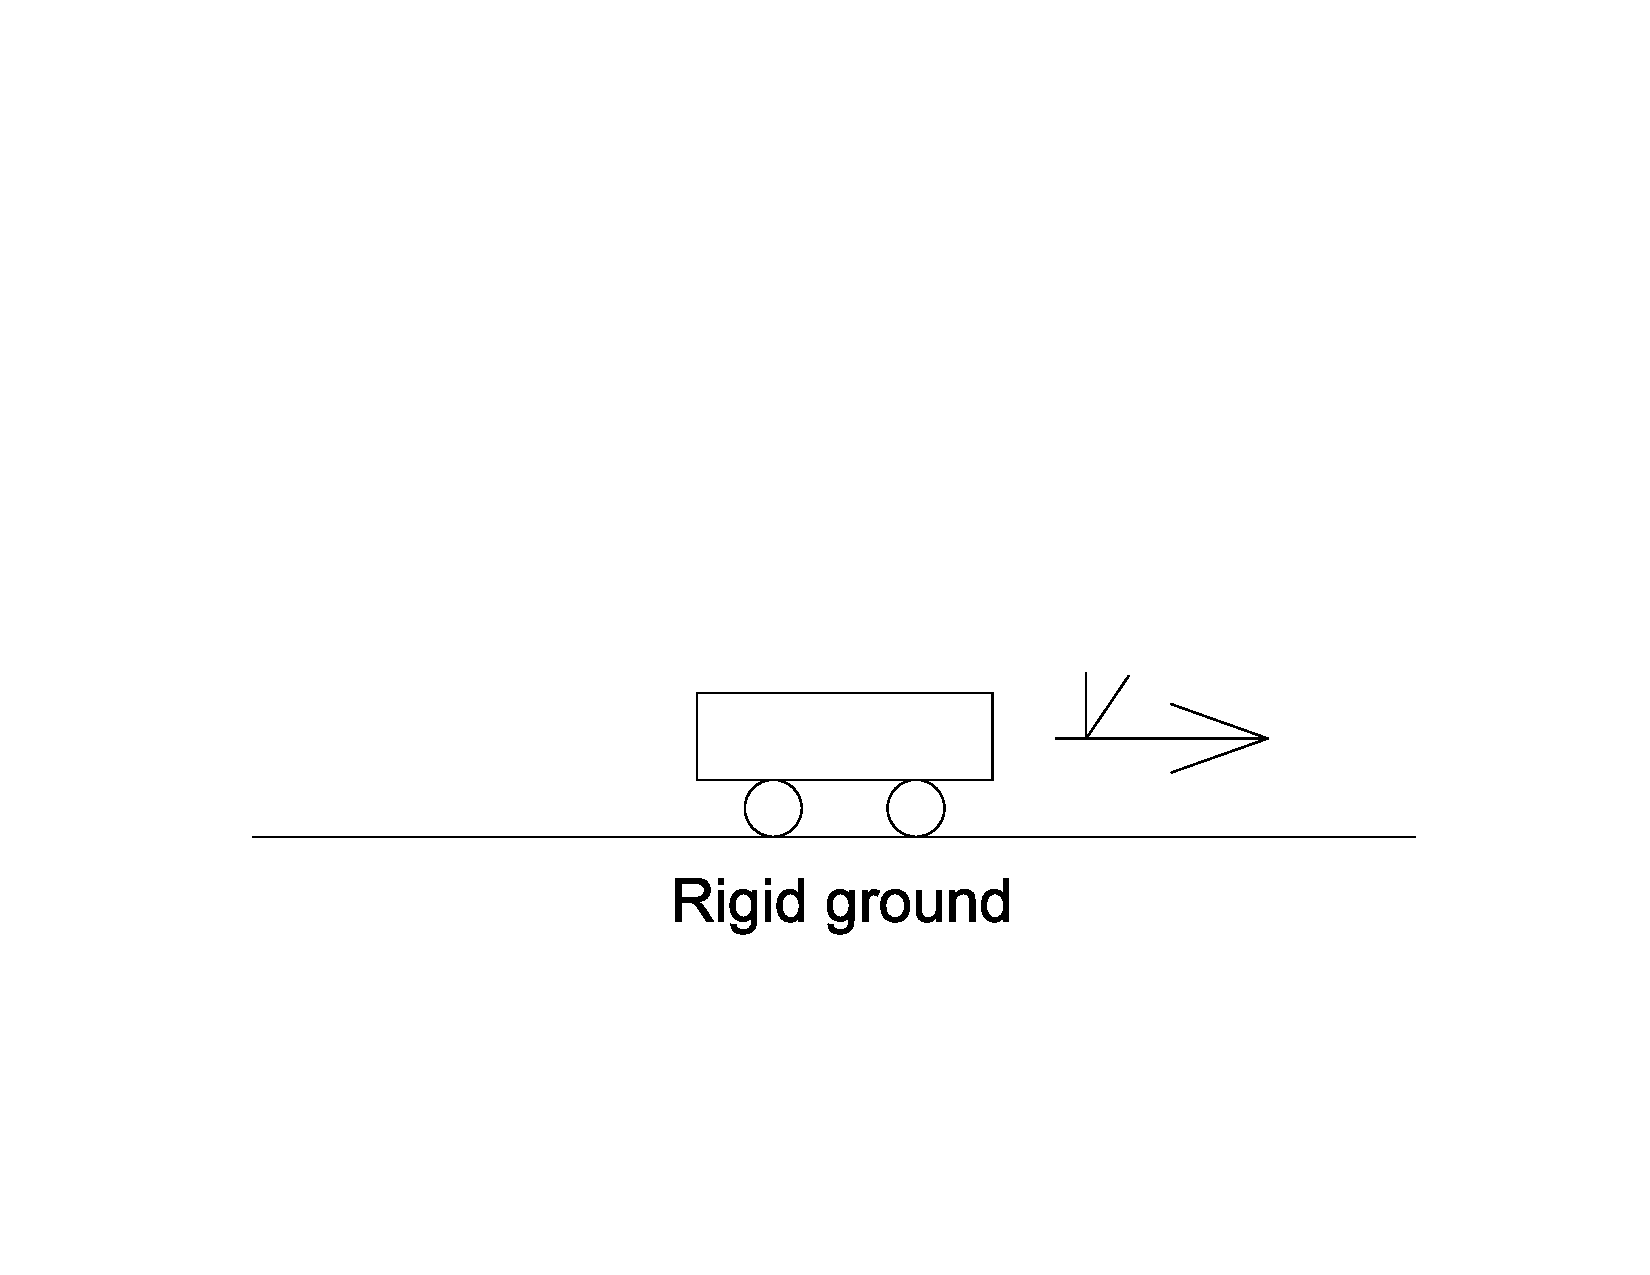
\includegraphics[width=0.8\textwidth]{trainmodellateralsimple.pdf}
%     \caption{Car model on rigid ground}
%     \label{fig:trainmodellateralsimple}
% \end{figure}

% An example of table of suspension parameters is listed in Fig.\ref{fig:suspensiondata}:

% \begin{figure}[h]
%     \centering
%     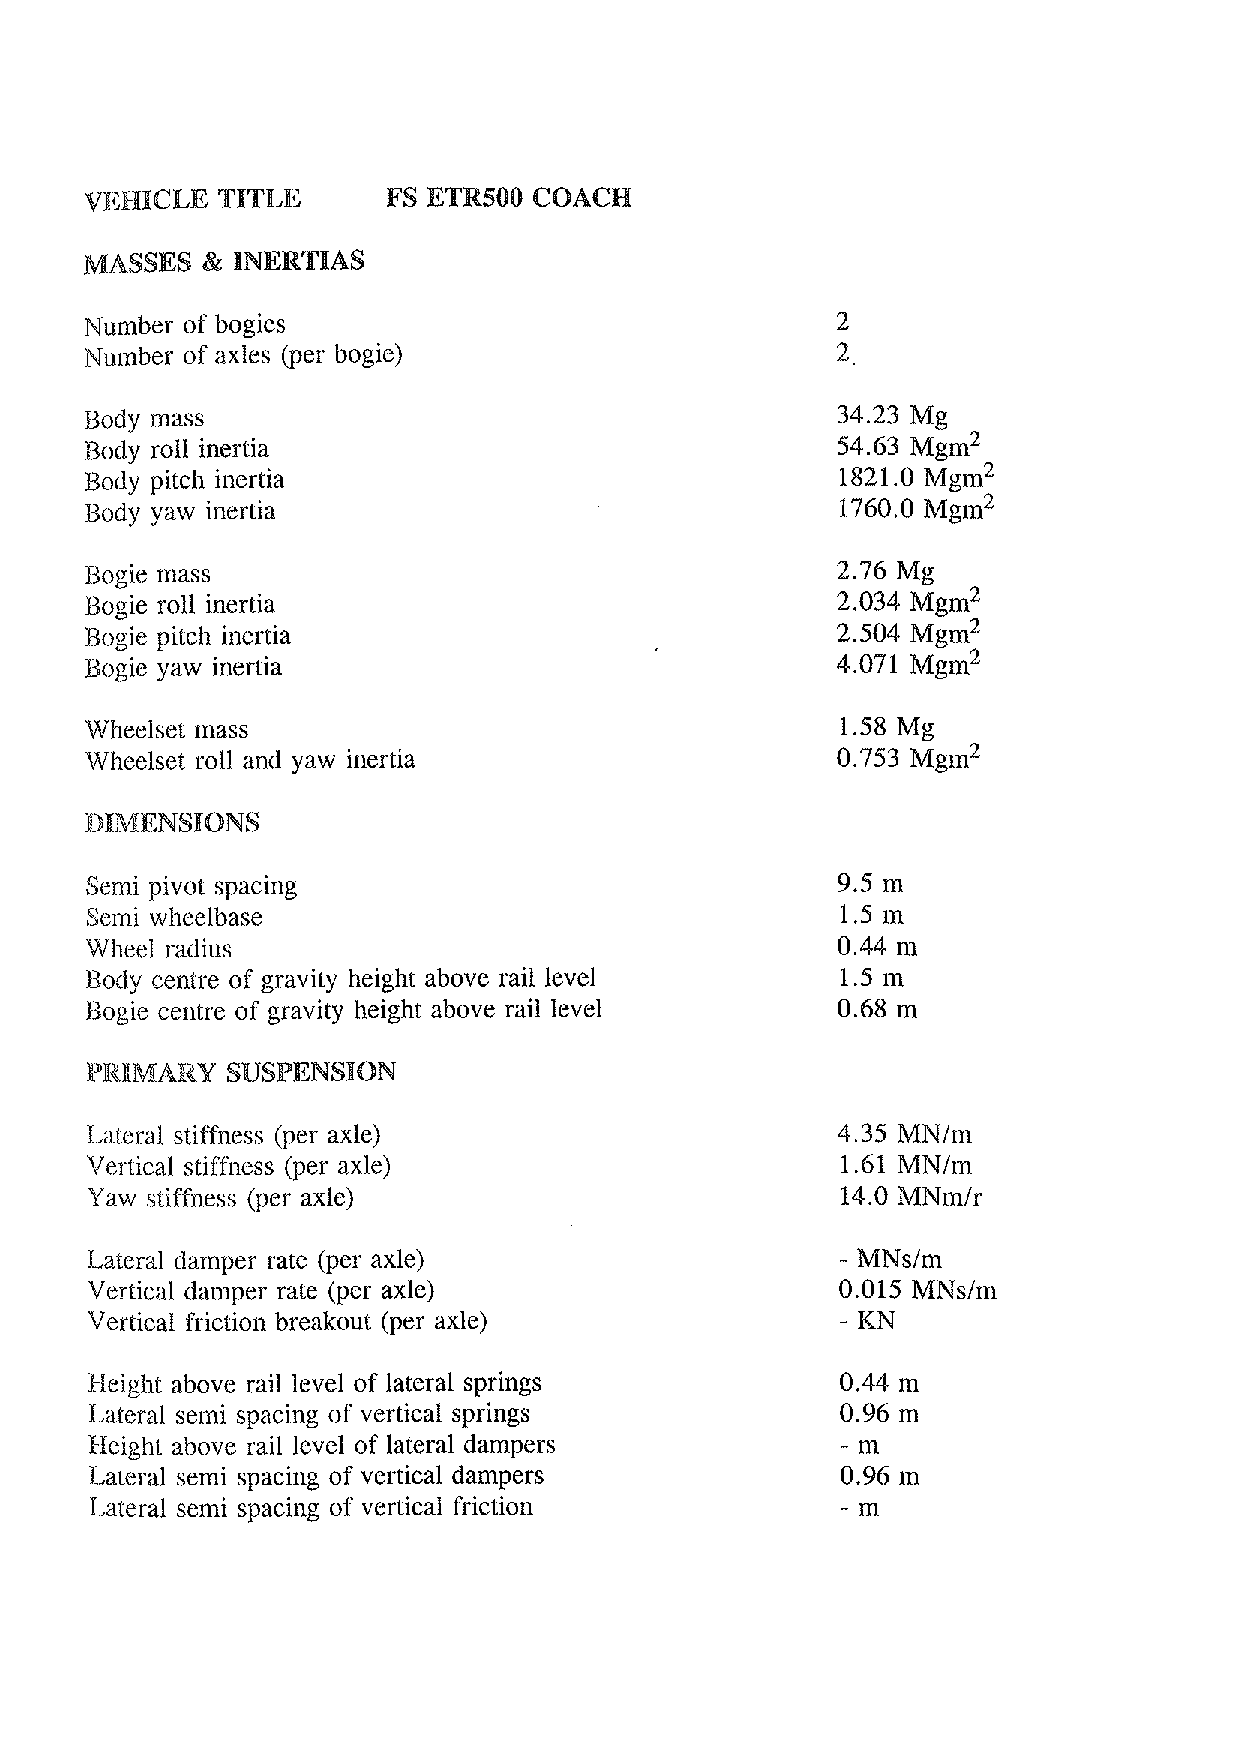
\includegraphics[width=0.8\textwidth]{suspensiondataexample.pdf}
%     \caption{example of table of suspension parameters extract from RP6\cite{d181}}
%     \label{fig:suspensiondata}
% \end{figure}

% Other parameter tables used are included in the appendix.

% \subsection{Kinetic movement of complete train}
% This step is to assemble car models defined in previous steps, trying to find out the influence of axle layouts on lateral frequency of single wheelset. Assemble rules are according to \cite{EC15528}. 

% The connections between cars are hinged. 

% \begin{figure}[h]
%     \centering
%     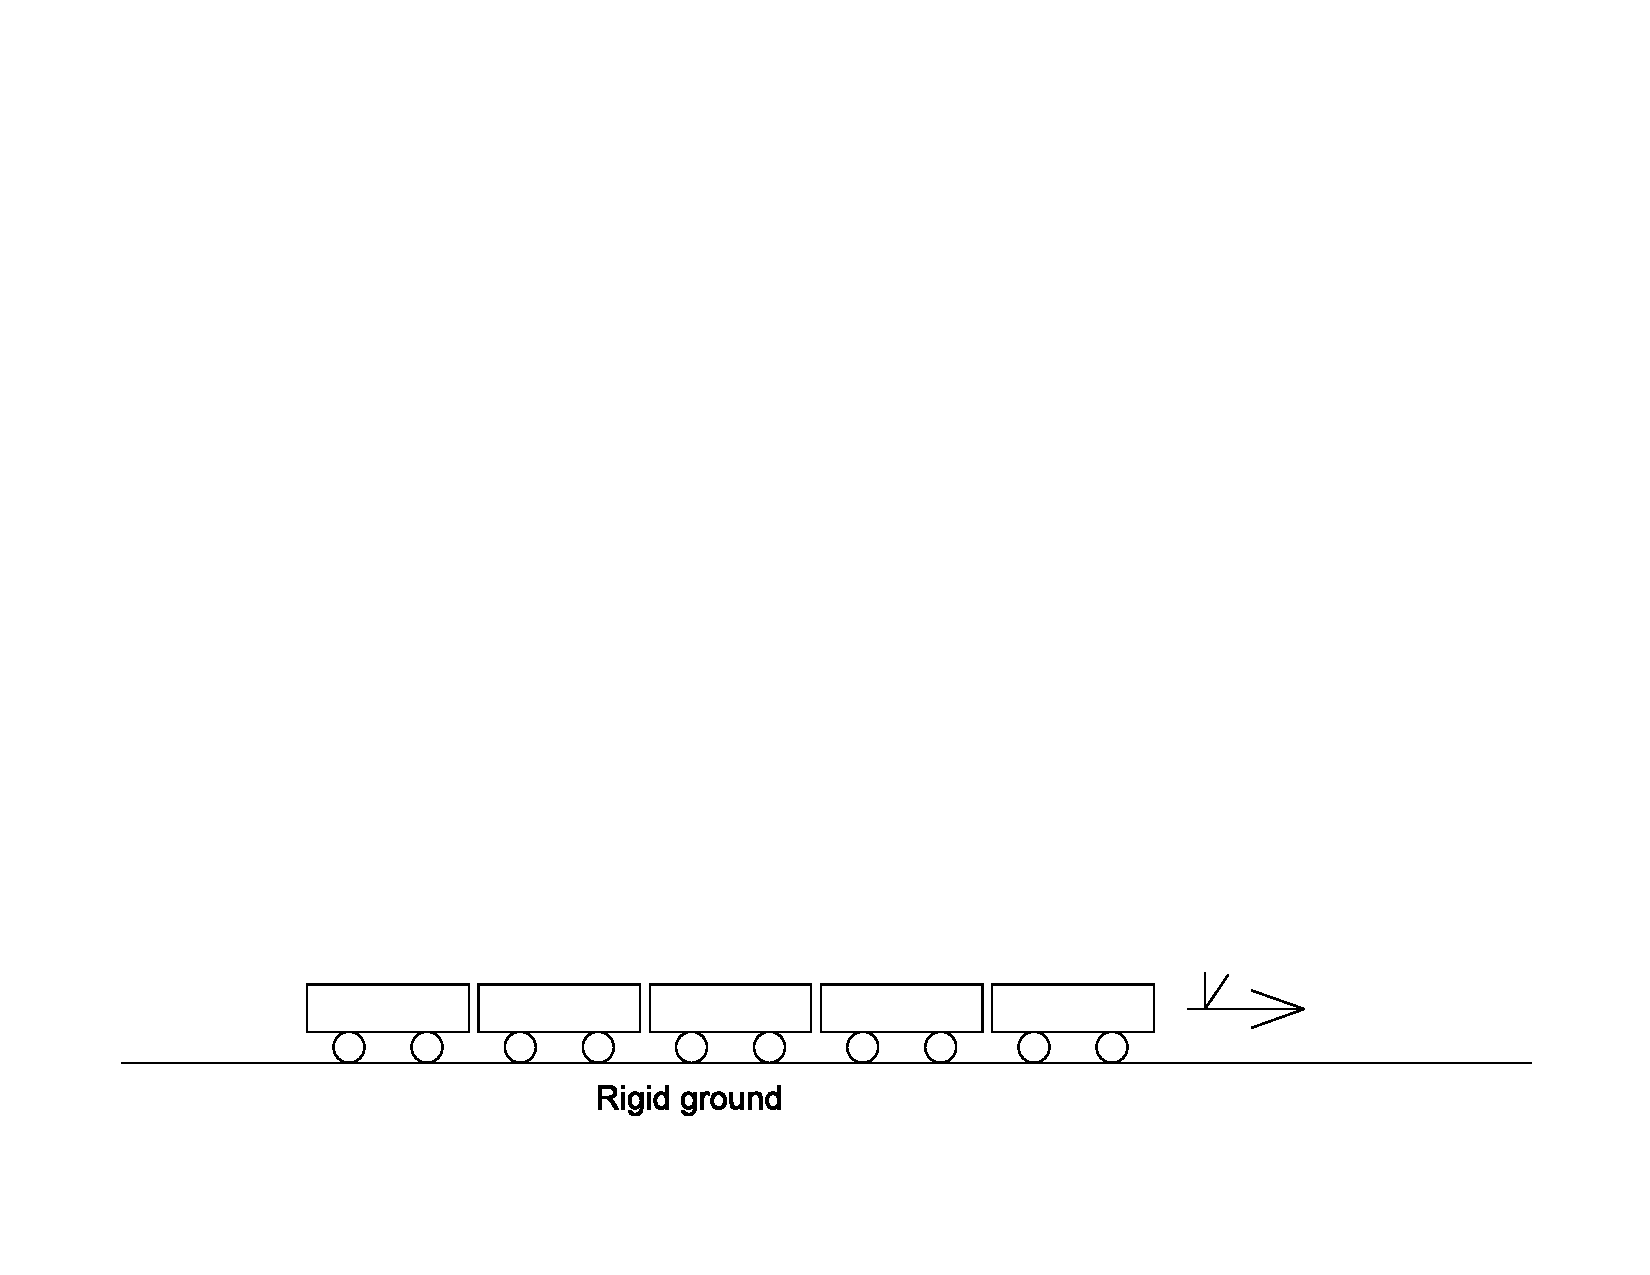
\includegraphics[width=0.8\textwidth]{trainmodellateralsimplecomplete.pdf}
%     \caption{Complete train model on rigid ground}
%     \label{fig:trainmodellateralsimplecomplete}
% \end{figure}


% \subsection{Coupled system modelling}
% From now on train model will move on bridge decks modelled as simply supported beams.

% Only one span of beam will be modelled because in RP6\cite[2.3]{d181} following statement mentioned 'there is no evidence that the resonant behaviour of the span has any effect on subsequent spans, since the resonant effects do not appear to grow from span to span.'. 

% Relative interfacing between track and bridge structure will be neglected. Thus ballast will not be modelled. Track and bridge structure will be modelled as a whole to shorten calculation time. 

% The interfacing of two systems will be investigated by following parametric studies.

% Till this step the basics of modelling are finished. Future parametric studies will use this 

% \begin{figure}[h]
%     \centering
%     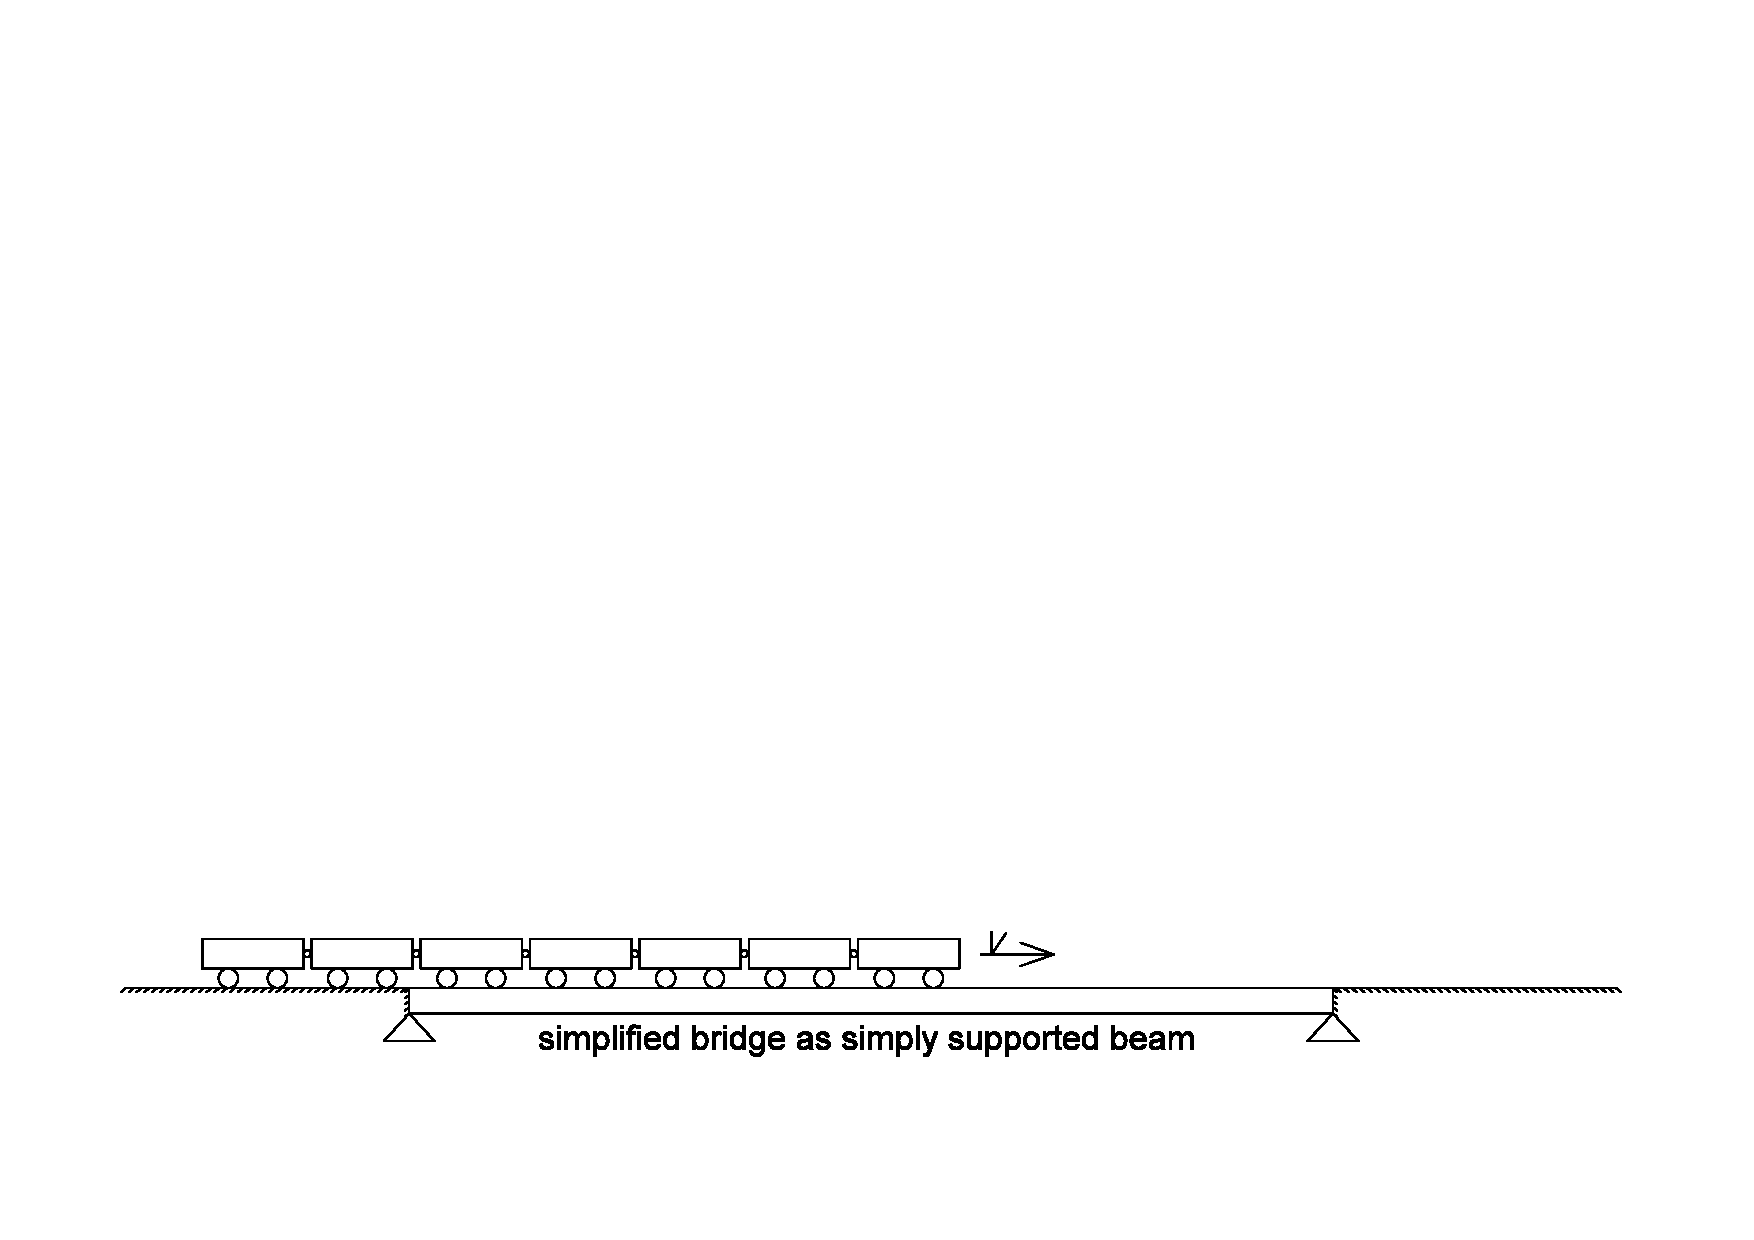
\includegraphics[width=0.8\textwidth]{trainmodellateral.pdf}
%     \caption{View of vehicle-Structure coupling model used in FEM software from the side3}
%     \label{fig:trainmodellateral}
% \end{figure}

% Parameters to be examined:
% \begin{enumerate}
% \item different layouts
% \item suspension system stiffness
% \item mass of the train
% \item track irregularities
% \item bridge span
% \item bridge mass
% \item bridge stiffness
% \end{enumerate}

\section{Effects investigated in wavelength study}

Effects investigated in this report will be the same effects investigated in DT 329, which is described in Sec.\ref{sec:resonanceinvestigated}. However, according to the statement in Sec.2.3[Summary of results] in the same report,

\begin{quote}
Even when the axle repeat frequency matches the first lateral bending mode of each span, there is no evidence that the resonant behaviour of the span and train has any effect on subsequent spans, since the resonant effects do not appear to grow from span to span.
\end{quote}

the third investigated resonance effect 'coincidence between the length of the span and the kinematic wavelength of the trailing vehicles' is neglected in this thesis. 


\section{Speed range of dynamic consideration}

The thesis will focus on normal speed trains because IV-Groep is only interested in normal speed train lines, which its projects are being built for. Higher boundary is set according to maximum speed allowed on Dutch railways, while lower boundary is set according to an estimation. The reason for a lower boundary speed is that dynamics issues for railway infrastructures increase with respect to vehicle speed, which means generally less concern is needed when the speed of train is low. It's certain that there exists a threshold of speed for every type of train that dynamic behaviour of them start to be a problem to concern but this threshold of speed varies from different scenarios. Till now no solid research can give a value to this threshold of speed so this is why estimation of lowest speed is adopted. 

My assumption of lower boundary of speed for consideration is 120 km/h. This is still very conservative because according to logic diagram Eurocode 1991-2\cite{EC12}, dynamic check is always needed when $V \geq 200km/h$ for vertical direction. Under same speed, the kinematic energy passed to bridge by running vehicle in vertical direction is apparently higher than that in lateral direction on a straight track. So it is believed that in lateral direction, the threshold will be even higher that 200 km/h according to Eurocode 1991-2. Value 120 km/h is taken according to \cite[Appendix F]{EC15528}: \textit{Speeds which do not require dynamic compatibility checks} where 120 km/h is the lowest speed can be found in the table, excluding special vehicle. This table is attached in this thesis in Appendix.\ref{app:speedsafe}.

Upper boundary for consideration:

Normal trains running on Dutch railway has a speed limit of 160 km/h so the upper boundary for speed is set to 160 km/h, which is also 44.44 m/s. 

$$ V_{max} = 44.44m/s $$

Lower boundary for consideration:

$$ V_{min} = 33.33m/s $$

However, it is strongly advised that future research investigate the lowest speed threshold for dynamic for consideration for train vehicles in the Netherlands due to the fact that the lower boundary used in this thesis in an assumption.

\section{Equivalent conicity used in this study}
According to \cite[Section.2.6]{esveld2001modern}, 

\begin{quote}
    Practical research has shown that over a period of time wheel profiles stabilise with wear at an equivalent conicity of 0.2 to 0.3. With regards to running stability, the equivalent conicity must remain below 0.4 and to ensure the centering effect it must be greater than 0.1.
\end{quote}

conicity range will be 0.2 to 0.3.

It is suggested that vehicle maintenance sector ensure wheels of train wheels stay in the safe zone of conicity. 


\section{Study on frequency of Klingel movement}

Klingel movement is proposed by Klingel which can well predict the moving trend of a single wheelset on a straight railway track. However, the kinematic movement of a certain wheelset assembled into a running train is different from the movement of a single free wheelset. This is due to multiple bodies interact with each other, introducing more complicated mechanism in wheel/rail interaction. 

This parametric study focuses on Klingel movement of a single wheelset. First part of the parametric study will try to discuss the relationship of Kiingle frequency of a wheelset and kinematic movement frequency of a whole train. Second part of the parametric study will use realistic data of Dutch railway/vehilces to assess the frequency bandwidth of Dutch native trains.

Parametric to be studied:

Speed of train, radius of the wheel and conicity of the wheel. 

Gauge distance is fixed to 1435mm according to UIC standard. 

Frequency is linear to speed if other parameters are fixed.

\section{Comparison between Klingle movement and train kinematic movement studied in D181 DT329}

By comparing the result from above parametric study and kinematic wavelength obtained by D181, presented as table.C2 in original report, parametric study results show close prediction for kinematic wavelength of freight train locomotive/coach/wagon. It's because freight train suspension system is simpler and stiffer compared to passenger train's, making the behaviour of train acts more similar to the behaviour of a single wheelset of bigger mass. However, results of  wavelength of single wheelset is 33\% shorter than kinematic wavelength of train because suspension system of passenger coaches are much more sophisticated. The wavelength of passenger coach is highly related to the characteristics of its suspension systems. These data is often difficult to obtain. 



The train parameter used in this part of parametric study is attached in the Appendix.\ref{app:mu}. 

% Table generated by Excel2LaTeX from sheet 'Sheet 1'
\begin{table}[htbp]
  \centering
  \caption{Add caption}
    \begin{tabular}{cccccccccccccccc}
    \toprule
    & Gauge & BWD & Radius & Conicity & Wavelength\_0() &Wavelength & Frequency(1m/s) \\
    \midrule
    BR CLASS 56 LOCOMOTIVE  & 1435 & 1500 & 290 & 0.0500 & 12.8175 & 18.5418 & 0.054 \\
    FS E444 LOCOMOTIVE  & 1435 & 1500 & 550 & 0.0500 & 17.6517 & 25.5349 & 0.039 \\
    FS ETR500 LOCOMOTIVE  & 1435 & 1500 & 550 & 0.0500 & 17.6517 & 25.5349 & 0.039 \\
    UIC FREIGHT WAGON (LADEN)  & 1435 & 1500 & 460 & 0.0500 & 16.1430 & 23.3524 & 0.043 \\
    FS ETR500 COACH  & 1435 & 1500 & 440 & 0.0500 & 15.7882 & 22.8391 & 0.044 \\
    UIC COACH  & 1435 & 1500 & 445 & 0.0500 & 15.8776 & 22.9685 & 0.044 \\
    \textbf{}       &       &       &       &       &       &       &  \\
    \textbf{} & 1435 & 1500 & 500 & 0.0250 & 23.8016 & 34.4313 & 0.029 \\
    \textbf{} & 1435 & 1500 & 500 & 0.2000 & 8.4151 & 12.1733 & 0.082 \\
    \textbf{} & 1435 & 1500 & 500 & 0.3000 & 6.8709 & 9.9395 & 0.101 \\
    \textbf{}       &       &       &       &       &       &       &  \\
    \textbf{} & 1435 & 1500 & 460 & 0.0250 & 22.8297 & 33.0253 & 0.030 \\
    \textbf{} & 1435 & 1500 & 460 & 0.2000 & 8.0715 & 11.6762 & 0.086 \\
    \textbf{} & 1435 & 1500 & 460 & 0.3000 & 6.5904 & 9.5336 & 0.105 \\
    \bottomrule
    \end{tabular}%
  \label{tab:addlabel}%
\end{table}%




\section{Assess of frequency bandwidth based on realistic data of Dutch Rail/Vehicle}

The wavelength of passenger coach is highly related to the characteristics of its suspension systems. These data is often difficult to obtain. To establish an easy approach, wavelength of passenger train calculated in this section will be multiplied by an amplification factor of 1.5. This value is obtain by train wavelength/wheelset wavelength ratio in previous parametric study. Please note this factor is an estimation. However, wavelength of freight train is not modified due to the conclusion that freight train's suspension system is stiff enough for the Klingle movement of a single wheelset to describe the kinematic movement of a whole freight train.

However, future research is highly recommended to be conducted to study the kinematic wavelength of complete vehicles in the Netherlands, using realistic data of their suspension systems.

Klingel's formula:
Klingel has done experiments and has given that the wavelength of a single wheelset:

$$ \lambda_0 = 2 \pi \sqrt{\frac{rG}{2\gamma} }$$

where:

G = Dynamic Gauge

r = Dynamic Wheels Radius

g = Conicity

For 2 wheelsets connected by a bogie:

$$ \lambda = \lambda_0 \sqrt{1+(\frac{I}{G})^2}  $$

where:

I = Rigid wheel base

Thus range of $\lambda$ is obtained by inputing data discussed in previous sections of this chapter.

Following plots are generated according to linear relationship between frequency and speed:

$$ f = v \frac{1}{\lambda} $$


\begin{figure}[h!]
\centering
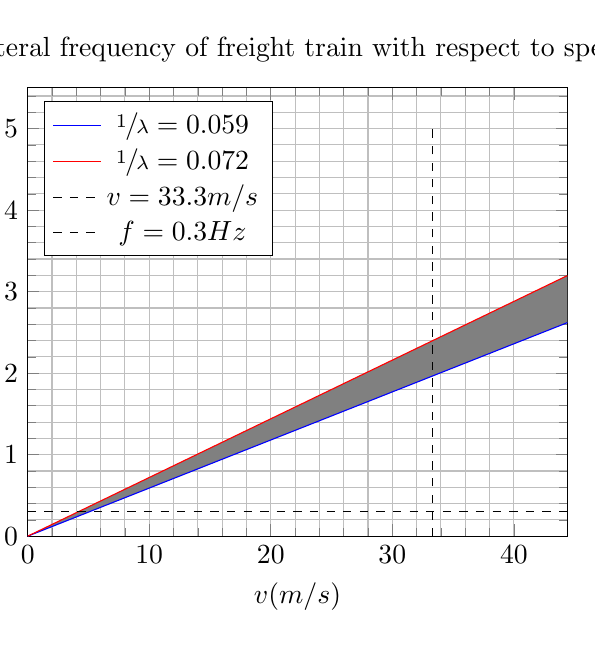
\begin{tikzpicture}[trim axis left, trim axis right]
\begin{axis}[
    title = {Lateral frequency of freight train with respect to speed},
    xlabel={$v(m/s)$},
    ylabel={$f(Hz)$},
    ymin = 0, xmin = 0, xmax = 44.4,
    legend entries={$\sfrac{1}{\lambda}=0.059$,$\sfrac{1}{\lambda} =0.072$,$v=33.3 m/s$,$f=0.3Hz$},
    grid = both,
    minor y tick num= 4,
    minor x tick num= 4,
    legend pos = north west,
]
\addplot[blue, domain = 0:44.4,samples=201,name path = A]{0.059*x};
\addplot[red, domain = 0:44.4,samples=201, name path = B]{0.072*x};
\addplot[mark=none, dashed]  coordinates {(33.3,0) (33.3,5) };
\addplot[domain = 0:44.4,samples=10,dashed]{0.3};
\addplot[gray] fill between[of=A and B];
\end{axis}
\end{tikzpicture}
\end{figure}

\begin{figure}[h!]
\centering
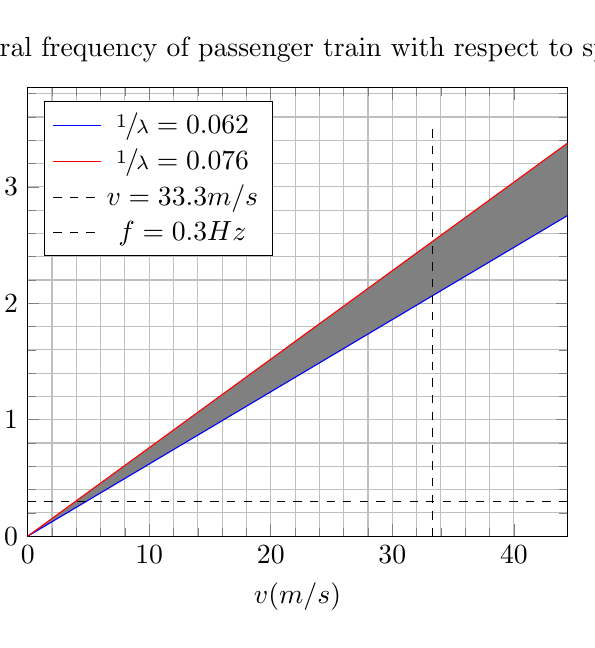
\begin{tikzpicture}[trim axis left, trim axis right]
\begin{axis}[
    title = {Lateral frequency of passenger train with respect to speed},
    xlabel={$v(m/s)$},
    ylabel={$f(Hz)$},
    ymin = 0, xmin = 0, xmax = 44.4,
    legend entries={$\sfrac{1}{\lambda}=0.062$,$\sfrac{1}{\lambda}=0.076$,$v=33.3 m/s$,$f=0.3Hz$},
    grid = both,
    minor y tick num= 4,
    minor x tick num= 4,
    legend pos = north west,
]
\addplot[blue, domain = 0:44.4,samples=201, name path = A]{0.062*x};
\addplot[red, domain = 0:44.4,samples=201, name path = B]{0.076*x};
\addplot[mark=none,dashed]  coordinates {(33.3,0) (33.3,3.5) };
\addplot[domain = 0:44.4,samples=10,dashed]{0.3};
\addplot[gray] fill between[of=A and B];
\end{axis}
\end{tikzpicture}

\end{figure}

\section{Study on frequency caused by axle repeat pattern}

Following wavelength of axle repeat pattern is obtained by extracting MU standards in \cite{EC15528}. Detailed information can be found in Appendix.\ref{app:mu}
% Table generated by Excel2LaTeX from sheet 'Axle repeat pattern'
\begin{table}[h!]
  \centering
  \caption{Wavelength of axle repeat pattern(m)}
    \begin{tabular}{rrrrrrrrr}
    \toprule
    \textbf{Type} & \textbf{L\_coa min} & \textbf{L\_coa max} & \textbf{2*L\_coa min } & \textbf{2*L\_coa max} \\
    \midrule
    \textbf{CB\_1} & 23.8  & 25.3  & 47.6  & 50.6 \\
    \textbf{CB\_2} & 25.3  & 27.5  & 50.6  & 55    \\
    \textbf{AB\_1} & 14.9  & 16    & 29.8  & 32     \\
    \textbf{AB\_2} & 18.8  & 19.5  & 37.6  & 39    \\
    \textbf{AB\_3} & 17    & 17.5  & 34    & 35   \\
    \textbf{AB\_4} & 18.7  & 19.2  & 37.4  & 38.4  \\
    \textbf{SA\_1} & 9.2   & 9.8   & 18.4  & 19.6  \\
    \textbf{SA\_2} & 12.8  & 13.5  & 25.6  & 27    \\
    \bottomrule
    \end{tabular}%
  \label{tab:wavelengthaxlerepeat}%
\end{table}%

Range of wavelength(m) of first repeat pattern mode:

$$ \lambda_{1stRepeat} \in (9.2,9.8) \cup (12.8,13.5) \cup (14.9, 16) \cup (17,17,5) \cup (18.7, 19.5) \cup (23.8,27.5)$$

Range of wavelength(m) of second repeat pattern mode:

$$ \lambda_{2ndRepeat} \in (18.4,19.6) \cup (25.6,27) \cup (29.8, 32) \cup (34,35) \cup (37.4, 39) \cup (37.6,55)$$

Range of frequency(Hz) yielded by dividing 1m/s with wavelength of first repeat pattern mode:

$$ \frac{1}{\lambda_{1stRepeat}} \in (0.036,0.042) \cup (0.051,0.053) \cup (0.057,0.059) \cup (0.063,0.067) \cup (0.074,0.078) \cup (0.102,0.109)   $$

Range of frequency(Hz) yielded by dividing 1m/s with wavelength of second repeat pattern mode:

$$ \frac{1}{\lambda_{2ndRepeat}} \in (0.018,0.021) \cup (0.026,0.027) \cup (0.029,0.029) \cup (0.031,0.034) \cup (0.037,0.039) \cup (0.051,0.054)   $$

Following plot is generated according to linear relationship between frequency and speed:

$$ f = v \frac{1}{\lambda_{repeat}} $$

\begin{figure}[h]
\centering
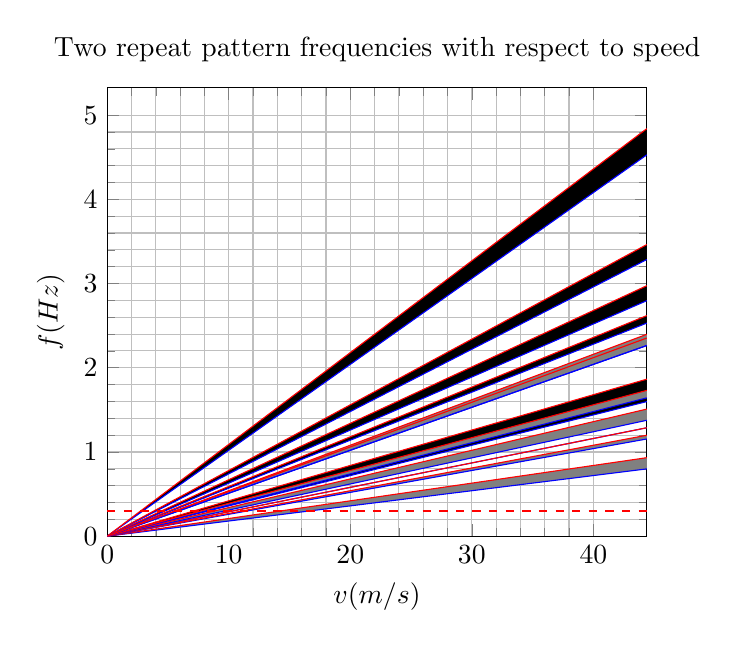
\begin{tikzpicture} 
    \begin{axis}[
    title = {Two repeat pattern frequencies with respect to speed},
    xlabel={$v(m/s)$},
    ylabel={$f(Hz)$},
    ymin = 0, xmin = 0, xmax = 44.4,
    %legend entries={$i=0.057$,$i=0.07$,$v=33.3 m/s$,$f=0.3Hz$},
    grid = both,
    minor y tick num= 4,
    minor x tick num= 4,
    ]
    \addplot[blue,name path=A,domain=0:44.4] {0.036*x};
    \addplot[red, name path=B,domain=0:44.4] {0.042*x};
    \addplot[black] fill between[of=A and B];
    \addplot[blue,name path=C,domain=0:44.4] {0.051*x};
    \addplot[red, name path=D,domain=0:44.4] {0.053*x};
    \addplot[black] fill between[of=C and D];
    \addplot[blue,name path=E,domain=0:44.4] {0.057*x};
    \addplot[red, name path=F,domain=0:44.4] {0.059*x};
    \addplot[black] fill between[of=E and F];
    \addplot[blue,name path=G,domain=0:44.4] {0.063*x};
    \addplot[red, name path=H,domain=0:44.4] {0.067*x};
    \addplot[black] fill between[of=G and H];
    \addplot[blue,name path=I,domain=0:44.4] {0.074*x};
    \addplot[red, name path=J,domain=0:44.4] {0.078*x};
    \addplot[black] fill between[of=I and J];
    \addplot[blue,name path=K,domain=0:44.4] {0.102*x};
    \addplot[red, name path=L,domain=0:44.4] {0.109*x};
    \addplot[black] fill between[of=K and L];
    \addplot[blue,name path=M,domain=0:44.4] {0.018*x};
    \addplot[red, name path=N,domain=0:44.4] {0.021*x};
    \addplot[gray] fill between[of=M and N];
    \addplot[blue,name path=O,domain=0:44.4] {0.026*x};
    \addplot[red, name path=P,domain=0:44.4] {0.027*x};
    \addplot[gray] fill between[of=O and P];
    \addplot[blue,name path=Q,domain=0:44.4] {0.029*x};
    \addplot[red, name path=R,domain=0:44.4] {0.029*x};
    \addplot[gray] fill between[of=Q and R];
    \addplot[blue,name path=S,domain=0:44.4] {0.031*x};
    \addplot[red, name path=T,domain=0:44.4] {0.034*x};
    \addplot[gray] fill between[of=S and T];
    \addplot[blue,name path=U,domain=0:44.4] {0.037*x};
    \addplot[red, name path=V,domain=0:44.4] {0.039*x};
    \addplot[gray] fill between[of=U and V];
    \addplot[blue,name path=W,domain=0:44.4] {0.051*x};
    \addplot[red, name path=X,domain=0:44.4] {0.054*x};
    \addplot[gray] fill between[of=W and X];
    \addplot[dashed,thick,red, domain=0:44.4] {0.3};
\end{axis}
\end{tikzpicture}
\end{figure}

\section{Conclusion of wavelength study}

This wavelength study illustrates a tool of obtaining danger zone for train speed for a specific bridge first lateral natural frequency. 

For example, if a bridge has a first lateral natural frequency of 0.3Hz:

\begin{enumerate}
\item To avoid resonance between freight train and bridge caused by kinematic frequency coincidence, speed of train should be regulated above 4m/s

\item To avoid resonance between passenger train and bridge caused by kinematic frequency coincidence, speed of train should be regulated above 5m/s

\item To avoid resonance caused by axle repeat pattern, speed of train should be regulated above 16m/s

\end{enumerate}

As a conclusion, if the speed of train is regulated above 16m/s, there won't be resonance between bridge and train.


\chapter{Fundamental of analytical approach to be adopted in practical checking method}
 
\section{Introduction}
This chapter aims to give a preliminary knowledge of a selected analytical model that simulates the perfect resonance scenario for railway bridge under lateral dynamic load. The knowledge contains the simplified model itself, its assumptions, field of application and explicit solutions. 

The output response of the solution to the analytical model is able to provide the maximum bridge response in worst case scenario. Thus it is sufficient to be adopted in practical purposes for verifications of lateral railway bridge dynamics.


\section{Overview}

To give a clear view of this chapter, following overview is created:

\begin{enumerate}
    \item The model, its assumptions and field of application. 
    \item Procedure of solution deduction
    \item Damping
\end{enumerate}

\section{The model, its assumptions and field of application}

\begin{figure}[h]
    \centering
    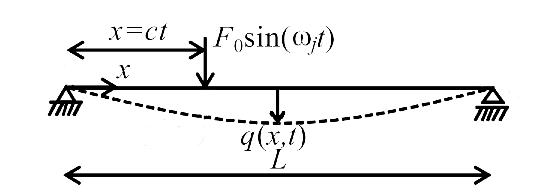
\includegraphics[width=0.5\textwidth]{harmonicloadbeam}
    \caption{Schematic representation of a generic beam crossed by a harmonic load}
    \label{fig:harmonicloadbeam}
\end{figure}

Presented in Figure.\ref{fig:harmonicloadbeam}, the model features a simply supported beam which is the simplification of bridge structure and a moving harmonic load introducing resonant dynamic effects caused by the presence of moving train.

The beam is assumed to be uniform in both geometry and material. The stiffness of the beam is the equivalent uniform lateral bending stiffness of the bridge. 

The load is moving in the same speed as the train. The magnitude of load amplitude in going to be discussed in the following chapter. And the load's self vibration frequency is equal to the first natural lateral bending frequency of the beam.


This model is valid for single span railway bridges that has a sinuous first natural lateral vibration shape.  

\section{Solution deduction}

Solution provided by Fryba\cite{fryba1999vibration} is used to analyse the problem. A harmonic moving along a beam is a fundamental dynamics topic and was first solved by S.P.Timoshenko. Fryba further deduced the basic results, and set them forth in the form of useful formulae. This model is used to simulate a perfect resonance scenario which yields conservative results for designing and checking of the dynamics behaviour of the bridge. Deduction procedure is extracted from \cite[Section II.2.1]{fryba1999vibration} and presented below.

\begin{quote}

The solution of the problem of a harmonic concentrated force moving at constant speed $c$ over a simply supported beam with span $l$ is carried out under the same assumptions as that discussed in Chap. 1. The time-variable concentrated force is of the form

\begin{equation}
    P(t) = Q \sin \Omega t
\end{equation}

where $Q$ is the amplitude and $\Omega$ is the circular frequency of the harmonic force. Vibration of the beam is then described by the equation

\begin{equation}\label{eq:equationofmotion}
    EJ\frac{\partial^4 v(x,t)}{\partial x^4} + \mu\frac{\partial^2 v(x,t)}{\partial t^2} +2\mu\omega_b \frac{\partial v(x,t)}{\partial t} = \delta(x-ct)Q\sin\Omega t 
\end{equation}

by the boundary conditions (1.2) and by the initial conditions (1.3). The symbols used in \ref{eq:equationofmotion} have the same meaning as those of Chap. 1.

Eq.\ref{eq:equationofmotion} together with conditions (1.2) and (1.3) will again be solved by the method of integral transformations. Following the Fourier sine transformation according to (1.9), Eqs.\ref{eq:equationofmotion} and (1.2) give

\begin{equation}
    \frac{d^2 V(j,t)}{d t^2} + 2\omega_b\frac{dV(j,t)}{dt} + \omega_{(j)}^2 V(j,t) = \frac{Q}{\mu} \sin\Omega t \sin j\omega t
\end{equation}

Solving the above with (1.3) by the Laplace-Carson transformation (1.15) - making use of Eq.(27.24) in doing so and of the notation

\begin{equation}
    \begin{tabular}{cc}
        $r_1 = \Omega + j\omega$; & $r_2 = \Omega - j\omega$ \\
    \end{tabular}
\end{equation}

we get

\begin{equation}\label{eq:V*}
    V^* (j,p) = \frac{Q}{2\mu} (\frac{1}{p^2+r_2^2}-\frac{1}{p^2+r_1^2})\frac{p^2}{(p+\omega_b)^2+\omega_{(j)}^{'2}}
\end{equation}

After inverse transformations of Eq.\ref{eq:V*} according to (27.24) and (1.9) the required result for $t \leq T$ is

\begin{dmath}\label{eq:v(x,t)complicated}
    v(x,t) = \sum_{j=1}^{\infty} \frac{Q}{\mu l}\{\frac{1}{(\omega_{(j)}^2 - r_2^2)+4\omega_b^2r_2^2}[(\omega_{j}^2-r_2^2])(\cos r_2t-e^{-\omega_bt}\cos \omega_{(j)}^' t) + 2\omega_b r_2 \sin r_2 t - \frac{\omega_b}{\omega_{(j)}^'}(\omega_{(j)}^2 + r_2^2)e^{-\omega_b t}\sin \omega_{(j)}^'t]-\frac{1}{(\omega_{(J)}^2 - r_1^2)^2 + 4\omega_b^2r_1^2}[(\omega_{(j)}^2-r_1^2)(\cos r_1t-e^{-\omega_b t}\cos\omega{(j)}^'t)+2\omega_b r_1 \sin r_1 t- \frac{\omega_b}{\omega_{(j)}^'}(\omega_{(j)}^2+r_1^2)e^{-\omega_b t}\sin \omega_{(j)}^' t]\}\sin\frac{j\pi x}{l}
\end{dmath}

We shall now simplify Eq.\ref{eq:v(x,t)complicated} to fit the case most frequently met with in practical applications. Thus, for example, it is entirely satisfactory to use only the first of its terms($j=1$); further, as we know from Chap. 1, parameters $\alpha$ and $\beta$ are usually much smaller than 1 ($\alpha = \sfrac{\omega}{\omega_{(1)}} \ll 1$, $\beta = \sfrac{\omega_b}{\omega_{(1)}} \ll 1$). And finally, since in practice a harmonic force is always accompanied by a constant force $P$, we shall introduce in \ref{eq:v(x,t)complicated} also the deflection $v_0$ according to (1.21). Following these simplifications Eq.(2.6) takes on the form

\begin{dmath}\label{eq:v(x,t)withP}
v(x,t) = v_0 \frac{Q}{p}\frac{\omega_{(1)}^2}{\Omega^2}\frac{1}{(\frac{\omega_{(1)}^2}{\Omega^2}-1)^2+4(\frac{\omega^2}{\Omega^2}+\frac{\omega_b^2}{\Omega^2})}\{[(\frac{\omega_{(1)}^2}{\Omega^2}-1)^2+4\frac{\omega_b^2}{\Omega^2}]^{\sfrac{1}{2}} \sin (\Omega t + \varphi)\sin \omega t + 2\frac{\omega}{\Omega}(\cos \Omega t \cos \omega t - e^{-\omega_b t}\cos \omega_{(1)}t)\}\sin\frac{\pi x}{l}
\end{dmath}

where

\begin{equation}
    \tan \varphi = -\frac{2\sfrac{\omega_b}{\Omega}}{\sfrac{\omega_{(1)}^2}{\Omega^2}-1}
\end{equation}

The beam reaches the state of highest dynamic stressing in the region of resonance, i.e. whenever $\Omega$ is close or just equal to $\omega_{(1)}$, i.e.

\begin{equation}
    \Omega = \omega_{(1)}
\end{equation}

In such a case Eq.\ref{eq:v(x,t)withP} can further be simplified to 

\begin{equation}\label{eq:v(x,t)simplewithP}
    v(x,t) = v_0 \frac{Q\omega_{(1)}}{2P}\frac{\cos \omega_{(1)}t}{\omega^2+\omega_b^2}[\omega(\cos\omega t - e^{-\omega_b t})-\omega_b\sin\omega t]\sin\frac{\pi x}{l}
\end{equation}

\end{quote}

According to (1.21)

\begin{equation}
    v_0 = \frac{Pl^3}{48EJ} \approx \frac{2P}{\mu l \omega_{(1)}^2} = \frac{2Pl^3}{\pi ^4 EJ}
\end{equation}

substitute $v_0$ into Eq.\ref{eq:v(x,t)simplewithP}

\begin{equation}\label{eq:v(x,t)simpleharmonic}
    v(x,t) = \frac{l^3Q\omega_{(1)}}{\pi^4 EJ}\frac{\cos \omega_{(1)}t}{\omega^2+\omega_b^2}[\omega(\cos\omega t - e^{-\omega_b t})-\omega_b\sin\omega t]\sin\frac{\pi x}{l}
\end{equation}

And the mid-span response time-history for deflection is :

\begin{equation}\label{eq:v(x,t)simpleharmonic}
    v(\sfrac{l}{2},t) = \frac{l^3Q\omega_{(1)}}{\pi^4 EJ}\frac{\cos \omega_{(1)}t}{\omega^2+\omega_b^2}[\omega(\cos\omega t - e^{-\omega_b t})-\omega_b\sin\omega t]
\end{equation}

Above expression is the ready-to-use expression being adopted in practical checking method to be discussed in following chapter.

% \section{Refining analytical solution}
% In the case of lateral dynamics, constant force $P$ in Eq.\ref{eq:v(x,t)simplewithP} doesn't exist. 

% According to (1.21)

% \begin{equation}
%     v_0 = \frac{Pl^3}{48EJ} \approx \frac{2P}{\mu l \omega_{(1)}^2} = \frac{2Pl^3}{\pi ^4 EJ}
% \end{equation}


% substitute $v_0$ into Eq.\ref{eq:v(x,t)simplewithP}

% \begin{equation}\label{eq:v(x,t)simpleharmonic}
%     v(x,t) = \frac{l^3Q\omega_{(1)}}{\pi^4 EJ}\frac{\cos \omega_{(1)}t}{\omega^2+\omega_b^2}[\omega(\cos\omega t - e^{-\omega_b t})-\omega_b\sin\omega t]\sin\frac{\pi x}{l}
% \end{equation}

% with 

% \begin{dmath}
%     \begin{tabular}{c c c}
%         $Q = \{$\begin{tabular}{c c c}
%             $5.2064\cdot c^{0.7495}$ & $c \leq 120 km/h$ \\
%             $3.58\cdot c^{0.7495}$ & $120 km/h < c \leq  200 km/h $\\
%             $3.10\cdot c^{0.7495}$ & $200 km/h \leq c \leq 350 km/h$ \\ \end{tabular}; 

%         & $\omega_1 = \frac{\pi^2}{l^2}\sqrt{\frac{EJ}{\mu}}$ ;

%         & $\omega = \frac{\pi c}{l}$ \\ 
 
%     \end{tabular}
% \end{dmath}

% A matlab script is written to perform iterate calculations based on Eq.\ref{eq:v(x,t)simpleharmonic}. The code is titled as \textit{fog.m}, attached in Appendix.\ref{sec:matlabscripts}. 

\section{Damping}
Damping is an important parameter influencing the dynamic behaviour of a structure. \ref{eq:equationofmotion} uses a different form of damping expression $\omega_b$, which can be converted from normal damping coefficient. Equation of motion using damping coefficient:

\begin{equation}\label{eq:equationofmotiondampingcoefficient}
    EJ\frac{\partial^4 v(x,t)}{\partial x^4} + \mu\frac{\partial^2 v(x,t)}{\partial t^2} +\chi \frac{\partial v(x,t)}{\partial t} = \delta(x-ct)Q\sin\Omega t 
\end{equation}

where $\chi$ stands for damping coefficient. By comparing \ref{eq:equationofmotiondampingcoefficient} and \ref{eq:equationofmotion}:

\begin{equation}
    \omega_b = \frac{\chi}{2\mu}
\end{equation}

where:

$\omega_b$: circular frequency of damping

$\chi$: damping coefficient

$\mu$: mass per unit length of the bridge

also, in \cite[Page.704]{abu2000vibration} it is mentioned that:

\begin{quote}
    The external and internal damping of the beam are assumed to be proportional to the mass and stiffness of the beam respectively,i.e., $r_a = \gamma_1 \mu$.., where $\gamma_1$ and $\gamma_2$ are proportionality constants.
\end{quote}

thus:


\begin{equation}
    \omega_b = \frac{\gamma_1}{2}
\end{equation}

and it is mentioned in \cite[Eq.8]{abu2000vibration} that:

$$\zeta = \frac{\gamma_1}{\omega_1}$$

so:

$$\gamma_1 = \zeta\omega_1$$

so:

$$\omega_b = \frac{1}{2}\zeta\omega_1 = \frac{1}{2}\frac{\zeta\pi^2}{l^2}\sqrt{\frac{EJ}{\mu}}$$

where $\zeta$ is the structure damping ratio stated in EN1991-

Adopting $\zeta = 0.001$ for steel railway bridges. This $\zeta$ value is used among all DT329 simulations run files. See Figure.\ref{fig:examplerunfile} for example.

\section{Script structure}
\begin{figure}[h]
\centering
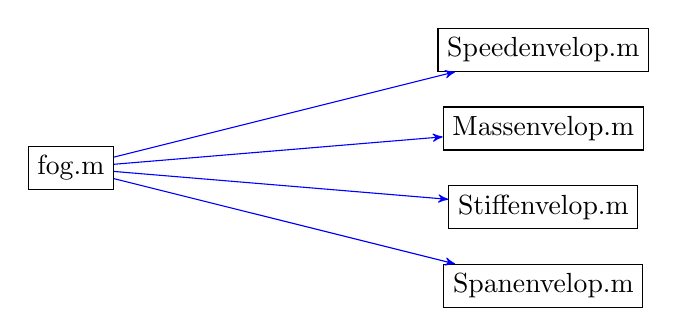
\begin{tikzpicture}
    \node[draw] (fog) at (0,0) {
        fog.m
    };
    \node[draw] (speed) at (6,1.5) {
        Speedenvelop.m
    };
    \node[draw] (mass) at (6,0.5) {
        Massenvelop.m
    };
    \node[draw] (stiff) at (6,-0.5) {
        Stiffenvelop.m
    };
    \node[draw] (span) at (6,-1.5) {
        Spanenvelop.m
    };
    \draw[->,draw=blue] (fog) to (speed);
    \draw[->,draw=blue] (fog) to (mass);
    \draw[->,draw=blue] (fog) to (stiff);
    \draw[->,draw=blue] (fog) to (span);
\end{tikzpicture}

\caption{Overview of script structure }
\label{fig:scriptstructure}
\end{figure}

In order to conduct the study efficiently, scripts in Matlab language are written to automate research procedure. See Appendix.\ref{sec:matlabscripts} for codes.

\textit{fog.m} is the core file for response calculation. This file is responsible for receiving bridge/train parameter input and yield time-history response for mid-span of the bridge. It also handles conversion of force amplitude from train speed. Calculation of bridge stiffness is also implemented, making it easier to input stiffness representing routine used in DT329.

Other scripts files are written to iterate fog.m in different parameters in order to conduct parametric study.

Read comments between the code for detailed explanation.
\textbf{remember to add comment}

\section{Comparison between analytical model and DT329 simulation results}


Several resonance phenomenon were produced during DT329 resonance study. By comparing with the output of reproduced resonance in DT329, the analytical model can be verified.

\subsection{First attempt}

\begin{figure}[h!]
    \centering
    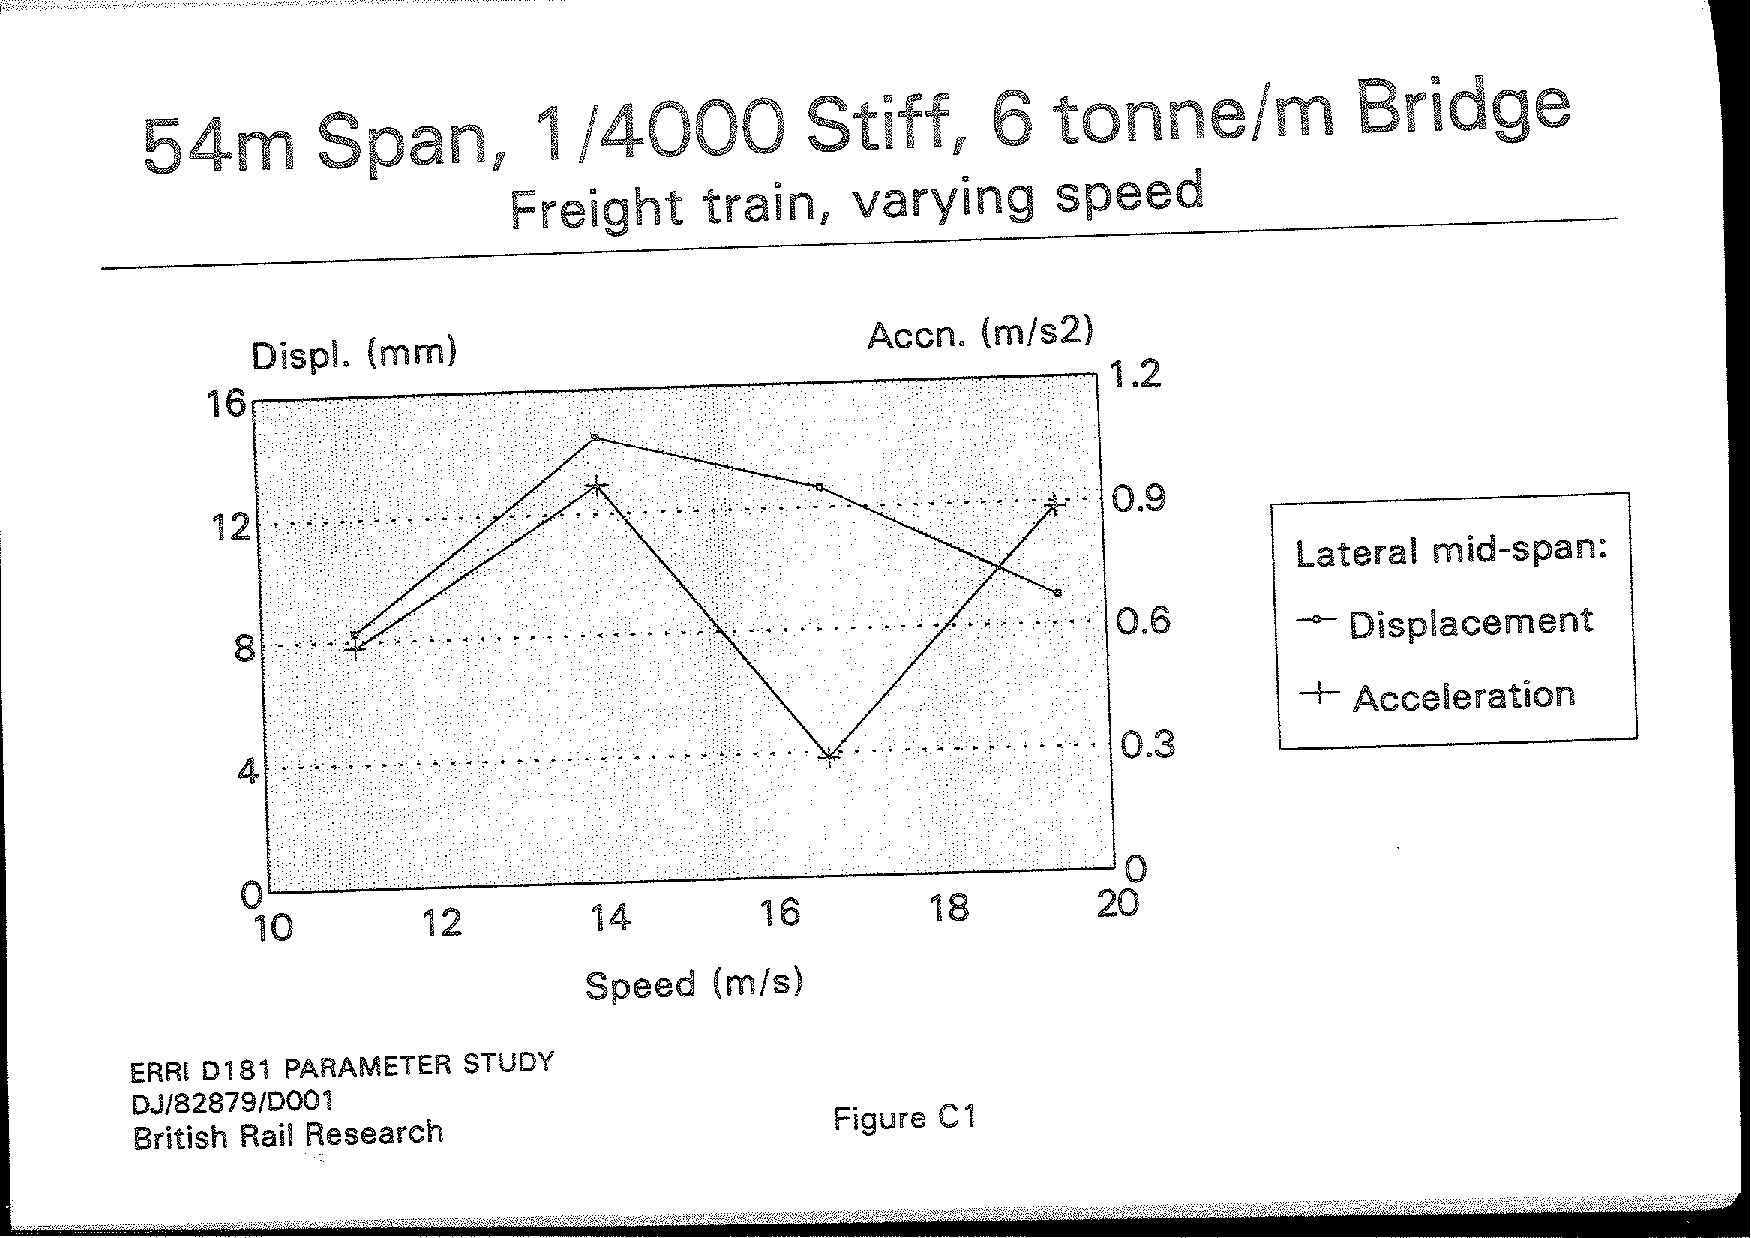
\includegraphics[width=0.8\textwidth]{c1}
    \caption{Figure C1 extracted from \cite{d181dt329} }
    \label{fig:c1}
\end{figure}

It can be observed in Figure.\ref{fig:c1} that the greatest resonance happened at train running at $14m/s$, on a bridge with following parameters: $l=54m$, $EJ=2.43e10Nm^2$, $mu=6000kg/m$. Displacement is approximately $15mm$ and acceleration is approximately $1.0m/s^2$.

A analytical run is done using the exactly same bridge parameters and using the load model proposed in Figure.\ref{fig:peaklateralforceregression}. 

\begin{figure}[h!]
\centering 
\newlength\figureheight 
\newlength\figurewidth 
\setlength\figureheight{6cm} 
\setlength\figurewidth{6cm} 
\input{./matlab/EJ24300000000L54mu6000c14.tikz} 
\caption{EJ24300000000L54mu6000c14.tikz} 
\label{fig:EJ24300000000L54mu6000c14} 
\end{figure}

Output is presented in Figure.\ref{fig:EJ24300000000L54mu6000c14}. Figure.\ref{fig:EJ24300000000L54mu6000c14} shows the time-history of mid-span response under model moving at $14m/s$, with maximum deflection at $17.1mm$ and maximum acceleration at $0.97 m/s^2$.

It can be concluded than analytical solution coincides well with the output of the simulations in the first comparison attempt because the output were close to each other and analytical output is slightly higher. This is acceptable because analytical model simulates a perfect resonance scenario while DT329 simulations takes multiple-axles into account. Axles may interfere with each other(different axle spacing) in the sense of harmoniously exciting the bridge, introducing disturbance into the development of resonance. So DT329 simulations are not perfect resonance scenarios and their output is supposed to be lower than analytical solutions.

\subsection{Second attempt}

The second attempt of comparison is conducted by extracting data from Figure.\ref{fig:c3}.  The bridge parameters are $l=54m$, $EJ=2.43e10Nm^2$, $mu=6000kg/m$, train is running at $60km/h$, converted to $16.67m/s$. 

\begin{figure}[h!]
    \centering
    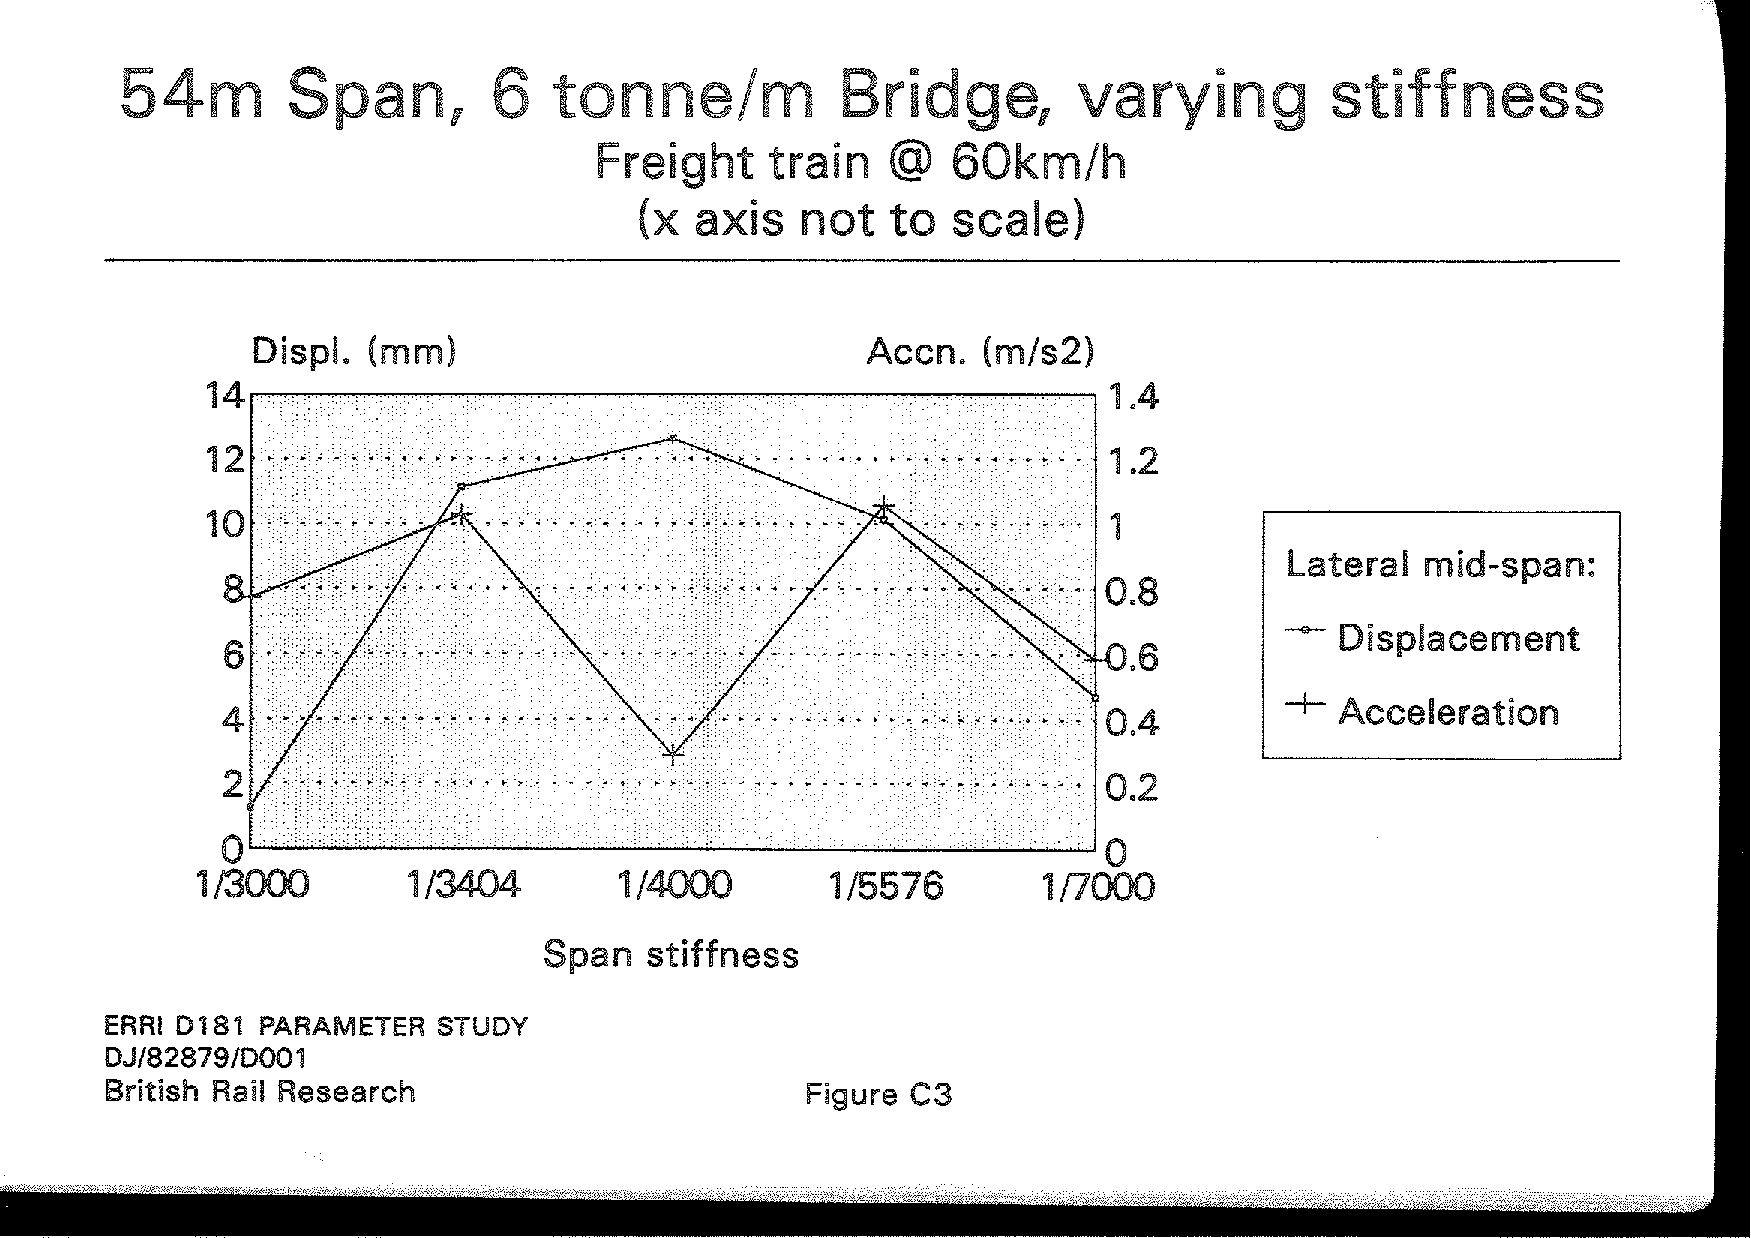
\includegraphics[width=0.8\textwidth]{c3}
    \caption{Figure C3 extracted from \cite{d181dt329} }
    \label{fig:c3}
\end{figure}

Maximum displacement in simulation is approximately $12.5mm$ and acceleration is approximately 0$.3m/s$. The acceleration value is surprisingly low with a step change. The reason causing this unexpected trend in acceleration is unknown, it is recommended to adopt $1.0m/s$ as a more general acceleration value. $1.0m/s$ is the acceleration for $1/3404$ stiffness and $1/5576$ stiffness. It can been seen that at these 2 stiffness, the resonance effect is already building up.

\begin{figure}[h!]
\centering 
\setlength\figureheight{6cm} 
\setlength\figurewidth{6cm} 
% This file was created by matlab2tikz v0.4.7 (commit d412d9f5e9b0b532484ca0001381d1809ceeed7a) running on MATLAB 8.3.
% Copyright (c) 2008--2014, Nico Schlmer <nico.schloemer@gmail.com>
% All rights reserved.
% Minimal pgfplots version: 1.3
% 
\begin{tikzpicture}

\begin{axis}[%
width=\figurewidth,
height=\figureheight,
scale only axis,
xmin=0,
xmax=3.5,
ymin=-1.5,
ymax=1.5,
title={Max Deflection:0.0218101765059296,Max Acceleration:1.06144343401643}
]
\addplot [color=blue,solid,forget plot]
  table[row sep=crcr]{%
0	0\\
0.00323935212957408	1.6826092635348e-06\\
0.00647870425914817	2.85000423783589e-06\\
0.00971805638872225	3.50491852469601e-06\\
0.0129574085182963	3.6515464421305e-06\\
0.0161967606478704	3.29552493404265e-06\\
0.0194361127774445	2.44391384728895e-06\\
0.0226754649070186	1.1051746059828e-06\\
0.0259148170365927	-7.10852685913743e-07\\
0.0291541691661668	-2.99297368135354e-06\\
0.0323935212957408	-5.72866573281395e-06\\
0.0356328734253149	-8.90410530599178e-06\\
0.038872225554889	-1.25041968287469e-05\\
0.0421115776844631	-1.65126029383019e-05\\
0.0453509298140372	-2.09117760886391e-05\\
0.0485902819436113	-2.56829914790215e-05\\
0.0518296340731854	-3.08063812635238e-05\\
0.0550689862027594	-3.62609700005339e-05\\
0.0583083383323335	-4.20247113002474e-05\\
0.0615476904619076	-4.80745256272663e-05\\
0.0647870425914817	-5.4386339214634e-05\\
0.0680263947210558	-6.09351240447422e-05\\
0.0712657468506299	-6.7694938851863e-05\\
0.074505098980204	-7.46389711002811e-05\\
0.077744451109778	-8.17395798913437e-05\\
0.0809838032393521	-8.8968339752089e-05\\
0.0842231553689262	-9.62960852575174e-05\\
0.0874625074985003	-0.000103692956438034\\
0.0907018596280744	-0.000111128444923029\\
0.0939412117576485	-0.000118571440771133\\
0.0971805638872225	-0.000125990279937226\\
0.100419916016797	-0.000133352792325925\\
0.103659268146371	-0.000140626350380882\\
0.106898620275945	-0.000147777918158962\\
0.110137972405519	-0.000154774100838114\\
0.113377324535093	-0.000161581194607494\\
0.116616676664667	-0.000168165236888292\\
0.119856028794241	-0.000174492056833511\\
0.123095380923815	-0.000180527326054941\\
0.126334733053389	-0.00018623660952546\\
0.129574085182963	-0.000191585416604847\\
0.132813437312537	-0.000196539252137311\\
0.136052789442112	-0.000201063667569024\\
0.139292141571686	-0.000205124312034106\\
0.14253149370126	-0.000208686983357636\\
0.145770845830834	-0.000211717678924522\\
0.149010197960408	-0.000214182646363302\\
0.152249550089982	-0.000216048433994211\\
0.155488902219556	-0.000217281940991263\\
0.15872825434913	-0.000217850467208399\\
0.161967606478704	-0.000217721762620207\\
0.165206958608278	-0.000216864076328191\\
0.168446310737852	-0.000215246205084023\\
0.171685662867427	-0.000212837541281792\\
0.174925014997001	-0.000209608120371803\\
0.178164367126575	-0.000205528667649108\\
0.181403719256149	-0.000200570644370612\\
0.184643071385723	-0.000194706293155244\\
0.187882423515297	-0.000187908682622448\\
0.191121775644871	-0.000180151751224977\\
0.194361127774445	-0.000171410350232766\\
0.197600479904019	-0.000161660285825506\\
0.200839832033593	-0.00015087836025236\\
0.204079184163167	-0.000139042412018195\\
0.207318536292741	-0.000126131355056591\\
0.210557888422316	-0.00011212521685085\\
0.21379724055189	-9.70051754652217e-05\\
0.217036592681464	-8.07535954495563e-05\\
0.220275944811038	-6.33540625816379e-05\\
0.223515296940612	-4.4791417412525e-05\\
0.226754649070186	-2.50517875813073e-05\\
0.22999400119976	-4.12261886681184e-06\\
0.233233353329334	1.80072950550656e-05\\
0.236472705458908	4.13477841785714e-05\\
0.239712057588482	6.59072750888103e-05\\
0.242951409718056	9.16927652637346e-05\\
0.24619076184763	0.000118709798783936\\
0.249430113977205	0.000146962443475515\\
0.252669466106779	0.000176453269510047\\
0.255908818236353	0.000207183329484358\\
0.259148170365927	0.000239152140001536\\
0.262387522495501	0.000272357664773275\\
0.265626874625075	0.000306796299262314\\
0.268866226754649	0.000342462856882396\\
0.272105578884223	0.000379350556771794\\
0.275344931013797	0.0004174510131551\\
0.278584283143371	0.000456754226306574\\
0.281823635272945	0.000497248575126965\\
0.285062987402519	0.000538920811344316\\
0.288302339532094	0.000581756055347882\\
0.291541691661668	0.000625737793662804\\
0.294781043791242	0.00067084787807187\\
0.298020395920816	0.000717066526389192\\
0.30125974805039	0.000764372324889227\\
0.304499100179964	0.000812742232393162\\
0.307738452309538	0.000862151586013224\\
0.310977804439112	0.000912574108554104\\
0.314217156568686	0.000963981917569171\\
0.31745650869826	0.00101634553606784\\
0.320695860827834	0.00106963390486897\\
0.323935212957409	0.00112381439659372\\
0.327174565086983	0.00117885283129004\\
0.330413917216557	0.00123471349367937\\
0.333653269346131	0.00129135915201491\\
0.336892621475705	0.00134875107853926\\
0.340131973605279	0.00140684907152809\\
0.343371325734853	0.00146561147890495\\
0.346610677864427	0.00152499522341093\\
0.349850029994001	0.00158495582931186\\
0.353089382123575	0.0016454474506241\\
0.356328734253149	0.00170642290083871\\
0.359568086382723	0.00176783368412276\\
0.362807438512298	0.00182963002797489\\
0.366046790641872	0.00189176091731123\\
0.369286142771446	0.00195417412995659\\
0.37252549490102	0.00201681627351433\\
0.375764847030594	0.00207963282358741\\
0.379004199160168	0.0021425681633219\\
0.382243551289742	0.00220556562424294\\
0.385482903419316	0.00226856752835207\\
0.38872225554889	0.00233151523145395\\
0.391961607678464	0.00239434916767907\\
0.395200959808038	0.00245700889516823\\
0.398440311937612	0.00251943314288353\\
0.401679664067187	0.00258155985850959\\
0.404919016196761	0.00264332625740758\\
0.408158368326335	0.00270466887258409\\
0.411397720455909	0.00276552360563557\\
0.414637072585483	0.00282582577862832\\
0.417876424715057	0.00288551018687342\\
0.421115776844631	0.00294451115255464\\
0.424355128974205	0.00300276257916716\\
0.427594481103779	0.00306019800672369\\
0.430833833233353	0.00311675066768431\\
0.434073185362927	0.00317235354356519\\
0.437312537492501	0.00322693942218121\\
0.440551889622076	0.00328044095547637\\
0.44379124175165	0.00333279071789577\\
0.447030593881224	0.00338392126525207\\
0.450269946010798	0.00343376519403893\\
0.453509298140372	0.00348225520114357\\
0.456748650269946	0.00352932414390992\\
0.45998800239952	0.00357490510050376\\
0.463227354529094	0.00361893143053049\\
0.466466706658668	0.0036613368358562\\
0.469706058788242	0.00370205542158229\\
0.472945410917816	0.00374102175712357\\
0.47618476304739	0.00377817093733962\\
0.479424115176965	0.00381343864366919\\
0.482663467306539	0.00384676120521689\\
0.485902819436113	0.00387807565974187\\
0.489142171565687	0.00390731981449753\\
0.492381523695261	0.00393443230687182\\
0.495620875824835	0.00395935266477742\\
0.498860227954409	0.00398202136674123\\
0.502099580083983	0.00400237990164264\\
0.505338932213557	0.00402037082805039\\
0.508578284343131	0.00403593783310773\\
0.511817636472705	0.00404902579091602\\
0.51505698860228	0.00405958082036708\\
0.518296340731854	0.00406755034237494\\
0.521535692861428	0.0040728831364579\\
0.524775044991002	0.00407552939662228\\
0.528014397120576	0.00407544078649951\\
0.53125374925015	0.00407257049368889\\
0.534493101379724	0.00406687328325851\\
0.537732453509298	0.00405830555035763\\
0.540971805638872	0.00404682537189428\\
0.544211157768446	0.00403239255723228\\
0.54745050989802	0.00401496869786279\\
0.550689862027594	0.00399451721600588\\
0.553929214157169	0.00397100341209858\\
0.557168566286743	0.00394439451112634\\
0.560407918416317	0.0039146597077557\\
0.563647270545891	0.00388177021022691\\
0.566886622675465	0.00384569928296584\\
0.570125974805039	0.00380642228787546\\
0.573365326934613	0.00376391672426816\\
0.576604679064187	0.00371816226740093\\
0.579844031193761	0.00366914080557662\\
0.583083383323335	0.00361683647577511\\
0.586322735452909	0.00356123569777963\\
0.589562087582484	0.0035023272067643\\
0.592801439712058	0.00344010208430995\\
0.596040791841632	0.00337455378781658\\
0.599280143971206	0.00330567817828182\\
0.60251949610078	0.00323347354641585\\
0.605758848230354	0.0031579406370645\\
0.608998200359928	0.00307908267191345\\
0.612237552489502	0.00299690537044745\\
0.615476904619076	0.00291141696914012\\
0.61871625674865	0.00282262823885063\\
0.621955608878224	0.00273055250040535\\
0.625194961007798	0.00263520563834343\\
0.628434313137373	0.0025366061128068\\
0.631673665266947	0.00243477496955644\\
0.634913017396521	0.00232973584809794\\
0.638152369526095	0.00222151498790079\\
0.641391721655669	0.00211014123269746\\
0.644631073785243	0.00199564603284921\\
0.647870425914817	0.00187806344576745\\
0.651109778044391	0.00175743013438066\\
0.654349130173965	0.00163378536363827\\
0.657588482303539	0.00150717099504439\\
0.660827834433113	0.00137763147921578\\
0.664067186562687	0.00124521384645979\\
0.667306538692262	0.00110996769536934\\
0.670545890821836	0.000971945179433906\\
0.67378524295141	0.000831200991666317\\
0.677024595080984	0.000687792347247184\\
0.680263947210558	0.000541778964189856\\
0.683503299340132	0.000393223042030495\\
0.686742651469706	0.000242189238549288\\
0.68998200359928	8.87446445300665e-05\\
0.693221355728854	-6.70412434325735e-05\\
0.696460707858428	-0.000225096552068381\\
0.699700059988002	-0.000385347062497029\\
0.702939412117576	-0.000547716243210795\\
0.706178764247151	-0.000712125284959685\\
0.709418116376725	-0.000878493137522973\\
0.712657468506299	-0.00104673654834937\\
0.715896820635873	-0.00121677010304707\\
0.719136172765447	-0.00138850626770317\\
0.722375524895021	-0.00156185543301074\\
0.725614877024595	-0.00173672596018031\\
0.728854229154169	-0.00191302422861135\\
0.732093581283743	-0.00209065468529783\\
0.735332933413317	-0.00226951989594052\\
0.738572285542891	-0.00244952059773778\\
0.741811637672465	-0.0026305557538246\\
0.74505098980204	-0.0028125226093291\\
0.748290341931614	-0.00299531674901397\\
0.751529694061188	-0.00317883215646908\\
0.754769046190762	-0.00336296127482061\\
0.758008398320336	-0.00354759506892046\\
0.76124775044991	-0.00373262308897873\\
0.764487102579484	-0.00391793353560085\\
0.767726454709058	-0.00410341332618987\\
0.770965806838632	-0.00428894816267314\\
0.774205158968206	-0.00447442260051168\\
0.77744451109778	-0.00465972011894953\\
0.780683863227355	-0.00484472319245914\\
0.783923215356929	-0.00502931336333801\\
0.787162567486503	-0.00521337131541087\\
0.790401919616077	-0.00539677694879049\\
0.793641271745651	-0.00557940945564974\\
0.796880623875225	-0.00576114739695608\\
0.800119976004799	-0.00594186878011934\\
0.803359328134373	-0.00612145113750253\\
0.806598680263947	-0.00629977160574475\\
0.809838032393521	-0.00647670700584438\\
0.813077384523095	-0.00665213392395034\\
0.816316736652669	-0.00682592879280812\\
0.819556088782244	-0.00699796797380696\\
0.822795440911818	-0.00716812783957378\\
0.826034793041392	-0.00733628485705906\\
0.829274145170966	-0.00750231567105896\\
0.83251349730054	-0.00766609718811812\\
0.835752849430114	-0.0078275066607564\\
0.838992201559688	-0.00798642177196287\\
0.842231553689262	-0.00814272071989997\\
0.845470905818836	-0.00829628230276003\\
0.84871025794841	-0.00844698600371658\\
0.851949610077984	-0.00859471207591211\\
0.855188962207558	-0.00873934162742417\\
0.858428314337133	-0.00888075670615096\\
0.861667666466707	-0.00901884038455818\\
0.864907018596281	-0.00915347684422798\\
0.868146370725855	-0.00928455146015132\\
0.871385722855429	-0.009411950884705\\
0.874625074985003	-0.0095355631312543\\
0.877864427114577	-0.00965527765732251\\
0.881103779244151	-0.0097709854472688\\
0.884343131373725	-0.00988257909441563\\
0.887582483503299	-0.00998995288256758\\
0.890821835632873	-0.0100930028668632\\
0.894061187762447	-0.0101916269539019\\
0.897300539892022	-0.0102857249810894\\
0.900539892021596	-0.0103751987951418\\
0.90377924415117	-0.010459952329695\\
0.907018596280744	-0.0105398916819599\\
0.910257948410318	-0.0106149251883692\\
0.913497300539892	-0.0106849634991592\\
0.916736652669466	-0.0107499196518328\\
0.91997600479904	-0.0108097091434476\\
0.923215356928614	-0.0108642500016777\\
0.926454709058188	-0.0109134628545934\\
0.929694061187762	-0.0109572709991086\\
0.932933413317336	-0.0109956004680423\\
0.936172765446911	-0.0110283800957454\\
0.939412117576485	-0.0110555415822402\\
0.942651469706059	-0.0110770195558252\\
0.945890821835633	-0.011092751634096\\
0.949130173965207	-0.0111026784833346\\
0.952369526094781	-0.0111067438762209\\
0.955608878224355	-0.0111048947478204\\
0.958848230353929	-0.0110970812498036\\
0.962087582483503	-0.0110832568028543\\
0.965326934613077	-0.011063378147222\\
0.968566286742651	-0.0110374053913806\\
0.971805638872225	-0.0110053020587491\\
0.9750449910018	-0.0109670351324387\\
0.978284343131374	-0.0109225750979855\\
0.981523695260948	-0.010871895984035\\
0.984763047390522	-0.0108149754009397\\
0.988002399520096	-0.0107517945772387\\
0.99124175164967	-0.0106823383939839\\
0.994481103779244	-0.0106065954168835\\
0.997720455908818	-0.0105245579262305\\
1.00095980803839	-0.0104362219445887\\
1.00419916016797	-0.0103415872622087\\
1.00743851229754	-0.0102406574601472\\
1.01067786442711	-0.0101334399310656\\
1.01391721655669	-0.0100199458976843\\
1.01715656868626	-0.0099001904288723\\
1.02039592081584	-0.00977419245334942\\
1.02363527294541	-0.00964197477098575\\
1.02687462507498	-0.00950356406167851\\
1.03011397720456	-0.00935899089179224\\
1.03335332933413	-0.00920828971814783\\
1.03659268146371	-0.00905149888954797\\
1.03983203359328	-0.00888866064582835\\
1.04307138572286	-0.00871982111442507\\
1.04631073785243	-0.00854503030445084\\
1.049550089982	-0.00836434209827388\\
1.05278944211158	-0.00817781424059501\\
1.05602879424115	-0.00798550832502011\\
1.05926814637073	-0.00778748977812704\\
1.0625074985003	-0.00758382784102718\\
1.06574685062987	-0.00737459554842375\\
1.06898620275945	-0.00715986970517101\\
1.07222555488902	-0.00693973086033919\\
1.0754649070186	-0.00671426327879263\\
1.07870425914817	-0.00648355491028973\\
1.08194361127774	-0.00624769735611476\\
1.08518296340732	-0.0060067858332539\\
1.08842231553689	-0.0057609191361289\\
1.09166166766647	-0.00551019959590358\\
1.09490101979604	-0.00525473303738008\\
1.09814037192561	-0.00499462873350333\\
1.10137972405519	-0.00472999935749393\\
1.10461907618476	-0.00446096093263078\\
1.10785842831434	-0.00418763277970722\\
1.11109778044391	-0.00391013746218513\\
1.11433713257349	-0.00362860072907348\\
1.11757648470306	-0.00334315145555956\\
1.12081583683263	-0.00305392158142205\\
1.12405518896221	-0.00276104604725699\\
1.12729454109178	-0.00246466272854948\\
1.13053389322136	-0.00216491236762482\\
1.13377324535093	-0.00186193850351446\\
1.1370125974805	-0.00155588739977419\\
1.14025194961008	-0.00124690797029239\\
1.14349130173965	-0.00093515170312822\\
1.14673065386923	-0.000620772582421284\\
1.1499700059988	-0.000303927008414636\\
1.15320935812837	1.52262843646091e-05\\
1.15644871025795	0.000336526310722091\\
1.15968806238752	0.000659809920163839\\
1.1629274145171	0.000984911883967367\\
1.16616676664667	0.00131166498390716\\
1.16940611877624	0.00163990010258421\\
1.17264547090582	0.00196944631530881\\
1.17588482303539	0.00230013098348391\\
1.17912417516497	0.00263177984943535\\
1.18236352729454	0.00296421713263485\\
1.18560287942412	0.00329726562725981\\
1.18884223155369	0.00363074680103309\\
1.19208158368326	0.00396448089528578\\
1.19532093581284	0.00429828702618365\\
1.19856028794241	0.00463198328705854\\
1.20179964007199	0.00496538685178365\\
1.20503899220156	0.0052983140791323\\
1.20827834433113	0.00563058061805757\\
1.21151769646071	0.00596200151383054\\
1.21475704859028	0.00629239131497362\\
1.21799640071986	0.00662156418092462\\
1.22123575284943	0.00694933399036717\\
1.224475104979	0.00727551445016212\\
1.22771445710858	0.00759991920481361\\
1.23095380923815	0.00792236194640396\\
1.23419316136773	0.00824265652493034\\
1.2374325134973	0.00856061705897548\\
1.24067186562687	0.00887605804664537\\
1.24391121775645	0.00918879447670558\\
1.24715056988602	0.00949864193984762\\
1.2503899220156	0.00980541674001723\\
1.25362927414517	0.0101089360057353\\
1.25686862627475	0.0104090178013429\\
1.26010797840432	0.0107054812381001\\
1.26334733053389	0.0109981465850719\\
1.26658668266347	0.0112868353797282\\
1.26982603479304	0.0115713705381924\\
1.27306538692262	0.0118515764650669\\
1.27630473905219	0.0121272791627666\\
1.27954409118176	0.012398306340293\\
1.28278344331134	0.0126644875213779\\
1.28602279544091	0.0129256541519298\\
1.28926214757049	0.0131816397067136\\
1.29250149970006	0.0134322797951958\\
1.29574085182963	0.013677412266488\\
1.29898020395921	0.0139168773133206\\
1.30221955608878	0.0141505175749807\\
1.30545890821836	0.0143781782391466\\
1.30869826034793	0.0145997071425549\\
1.3119376124775	0.0148149548704326\\
1.31517696460708	0.0150237748546316\\
1.31841631673665	0.0152260234704002\\
1.32165566886623	0.0154215601317295\\
1.3248950209958	0.0156102473852101\\
1.32813437312537	0.0157919510023399\\
1.33137372525495	0.0159665400702197\\
1.33461307738452	0.0161338870805779\\
1.3378524295141	0.0162938680170643\\
1.34109178164367	0.0164463624407548\\
1.34433113377325	0.0165912535738102\\
1.34757048590282	0.016728428381232\\
1.35080983803239	0.0168577776506601\\
1.35404919016197	0.0169791960701592\\
1.35728854229154	0.0170925823039383\\
1.36052789442112	0.0171978390659554\\
1.36376724655069	0.0172948731913518\\
1.36700659868026	0.0173835957056714\\
1.37024595080984	0.0174639218918122\\
1.37348530293941	0.0175357713546672\\
1.37672465506899	0.0175990680834054\\
1.37996400719856	0.017653740511352\\
1.38320335932813	0.0176997215734214\\
1.38644271145771	0.0177369487610652\\
1.38968206358728	0.0177653641746922\\
1.39292141571686	0.0177849145735231\\
1.39616076784643	0.0177955514228435\\
1.399400119976	0.0177972309386178\\
1.40263947210558	0.0177899141294321\\
1.40587882423515	0.0177735668357321\\
1.40911817636473	0.017748159766326\\
1.4123575284943	0.0177136685321228\\
1.41559688062388	0.0176700736770792\\
1.41883623275345	0.0176173607063276\\
1.42207558488302	0.0175555201114632\\
1.4253149370126	0.0174845473929652\\
1.42855428914217	0.0174044430797337\\
1.43179364127175	0.0173152127457213\\
1.43503299340132	0.0172168670236428\\
1.43827234553089	0.0171094216157483\\
1.44151169766047	0.0169928973016437\\
1.44475104979004	0.0168673199431488\\
1.44799040191962	0.0167327204861816\\
1.45122975404919	0.0165891349596604\\
1.45446910617876	0.0164366044714176\\
1.45770845830834	0.0162751752011195\\
1.46094781043791	0.0161048983901902\\
1.46418716256749	0.0159258303287375\\
1.46742651469706	0.0157380323394821\\
1.47066586682663	0.0155415707586923\\
1.47390521895621	0.015336516914128\\
1.47714457108578	0.0151229471000022\\
1.48038392321536	0.0149009425489646\\
1.48362327534493	0.0146705894011211\\
1.4868626274745	0.0144319786700974\\
1.49010197960408	0.0141852062061621\\
1.49334133173365	0.0139303726564249\\
1.49658068386323	0.0136675834221253\\
1.4998200359928	0.0133969486130322\\
1.50305938812238	0.013118582998975\\
1.50629874025195	0.0128326059585279\\
1.50953809238152	0.0125391414248723\\
1.5127774445111	0.0122383178288641\\
1.51601679664067	0.0119302680393314\\
1.51925614877025	0.011615129300635\\
1.52249550089982	0.0112930431675208\\
1.52573485302939	0.0109641554372981\\
1.52897420515897	0.0106286160793786\\
1.53221355728854	0.0102865791622112\\
1.53545290941812	0.00993820277765244\\
1.53869226154769	0.00958364896281002\\
1.54193161367726	0.0092230836194029\\
1.54517096580684	0.00885667643067874\\
1.54841031793641	0.00848460077593413\\
1.55164967006599	0.00810703364268335\\
1.55488902219556	0.00772415553652277\\
1.55812837432513	0.0073361503887397\\
1.56136772645471	0.00694320546171656\\
1.56460707858428	0.00654551125218133\\
1.56784643071386	0.00614326139235799\\
1.57108578284343	0.00573665254907097\\
1.57432513497301	0.00532588432085998\\
1.57756448710258	0.00491115913316171\\
1.58080383923215	0.00449268213161713\\
1.58404319136173	0.00407066107356395\\
1.5872825434913	0.00364530621777516\\
1.59052189562088	0.00321683021250498\\
1.59376124775045	0.00278544798190633\\
1.59700059988002	0.00235137661088306\\
1.6002399520096	0.0019148352284425\\
1.60347930413917	0.00147604488961484\\
1.60671865626875	0.00103522845600599\\
1.60995800839832	0.000592610475052297\\
1.61319736052789	0.000148417058046412\\
1.61643671265747	-0.000297124242996376\\
1.61967606478704	-0.00074378455956044\\
1.62291541691662	-0.00119133383186894\\
1.62615476904619	-0.00163954093506829\\
1.62939412117576	-0.00208817380628482\\
1.63263347330534	-0.00253699957247973\\
1.63587282543491	-0.00298578467902936\\
1.63911217756449	-0.00343429501895479\\
1.64235152969406	-0.00388229606272706\\
1.64559088182364	-0.00432955298857116\\
1.64883023395321	-0.00477583081319399\\
1.65206958608278	-0.0052208945228589\\
1.65530893821236	-0.0056645092047309\\
1.65854829034193	-0.00610644017841551\\
1.66178764247151	-0.00654645312761345\\
1.66502699460108	-0.00698431423181477\\
1.66826634673065	-0.00741979029795449\\
1.67150569886023	-0.0078526488919518\\
1.6747450509898	-0.00828265847005618\\
1.67798440311938	-0.00870958850992214\\
1.68122375524895	-0.00913320964133504\\
1.68446310737852	-0.00955329377651115\\
1.6877024595081	-0.00996961423989421\\
1.69094181163767	-0.0103819458973714\\
1.69418116376725	-0.0107900652848321\\
1.69742051589682	-0.0111937507359934\\
1.70065986802639	-0.0115927825094145\\
1.70389922015597	-0.0119869429146266\\
1.70713857228554	-0.0123760164373006\\
1.71037792441512	-0.0127597898633797\\
1.71361727654469	-0.013138052402101\\
1.71685662867427	-0.013510595807833\\
1.72009598080384	-0.0138772145006562\\
1.72333533293341	-0.0142377056856132\\
1.72657468506299	-0.0145918694705576\\
1.72981403719256	-0.0149395089825305\\
1.73305338932214	-0.0152804304825931\\
1.73629274145171	-0.0156144434790479\\
1.73953209358128	-0.0159413608389782\\
1.74277144571086	-0.01626099889804\\
1.74601079784043	-0.0165731775684378\\
1.74925014997001	-0.0168777204450202\\
1.75248950209958	-0.01717445490943\\
1.75572885422915	-0.017463212232245\\
1.75896820635873	-0.0177438276730486\\
1.7622075584883	-0.0180161405783664\\
1.76544691061788	-0.018279994477412\\
1.76868626274745	-0.0185352371755799\\
1.77192561487702	-0.0187817208456314\\
1.7751649670066	-0.0190193021165142\\
1.77840431913617	-0.019247842159763\\
1.78164367126575	-0.0194672067734271\\
1.78488302339532	-0.0196772664634727\\
1.78812237552489	-0.0198778965226092\\
1.79136172765447	-0.0200689771064914\\
1.79460107978404	-0.0202503933072489\\
1.79784043191362	-0.0204220352242976\\
1.80107978404319	-0.0205837980323877\\
1.80431913617277	-0.0207355820468472\\
1.80755848830234	-0.0208772927859773\\
1.81079784043191	-0.0210088410305628\\
1.81403719256149	-0.021130142880457\\
1.81727654469106	-0.021241119808207\\
1.82051589682064	-0.0213416987096838\\
1.82375524895021	-0.0214318119516848\\
1.82699460107978	-0.0215113974164784\\
1.83023395320936	-0.02158039854326\\
1.83347330533893	-0.0216387643664937\\
1.83671265746851	-0.021686449551114\\
1.83995200959808	-0.0217234144245623\\
1.84319136172765	-0.0217496250056385\\
1.84643071385723	-0.0217650530301466\\
1.8496700659868	-0.0217696759733162\\
1.85290941811638	-0.0217634770689847\\
1.85614877024595	-0.0217464453255246\\
1.85938812237552	-0.0217185755385053\\
1.8626274745051	-0.0216798683000773\\
1.86586682663467	-0.0216303300050719\\
1.86910617876425	-0.0215699728538089\\
1.87234553089382	-0.0214988148516079\\
1.8755848830234	-0.0214168798050015\\
1.87882423515297	-0.0213241973146488\\
1.88206358728254	-0.0212208027649506\\
1.88530293941212	-0.0211067373103702\\
1.88854229154169	-0.020982047858465\\
1.89178164367127	-0.0208467870496352\\
1.89502099580084	-0.0207010132336\\
1.89826034793041	-0.0205447904426116\\
1.90149970005999	-0.0203781883614202\\
1.90473905218956	-0.0202012822940056\\
1.90797840431914	-0.0200141531270908\\
1.91121775644871	-0.019816887290459\\
1.91445710857828	-0.0196095767140917\\
1.91769646070786	-0.0193923187821526\\
1.92093581283743	-0.0191652162838421\\
1.92417516496701	-0.0189283773611467\\
1.92741451709658	-0.0186819154535135\\
1.93065386922615	-0.0184259492394793\\
1.93389322135573	-0.0181606025752862\\
1.9371325734853	-0.0178860044305169\\
1.94037192561488	-0.0176022888207865\\
1.94361127774445	-0.0173095947375267\\
1.94685062987403	-0.0170080660749017\\
1.9500899820036	-0.0166978515538981\\
1.95332933413317	-0.0163791046436285\\
1.95656868626275	-0.0160519834798952\\
1.95980803839232	-0.015716650781059\\
1.9630473905219	-0.0153732737612596\\
1.96628674265147	-0.0150220240410385\\
1.96952609478104	-0.0146630775554123\\
1.97276544691062	-0.0142966144594518\\
1.97600479904019	-0.0139228190314166\\
1.97924415116977	-0.0135418795735036\\
1.98248350329934	-0.0131539883102638\\
1.98572285542891	-0.0127593412847463\\
1.98896220755849	-0.012358138252428\\
1.99220155968806	-0.0119505825729901\\
1.99544091181764	-0.0115368811000032\\
1.99868026394721	-0.0111172440685838\\
2.00191961607678	-0.0106918849810872\\
2.00515896820636	-0.010261020490901\\
2.00839832033593	-0.00982487028440838\\
2.01163767246551	-0.00938365696118554\\
2.01487702459508	-0.00893760591250549\\
2.01811637672466	-0.00848694519821576\\
2.02135572885423	-0.00803190542206208\\
2.0245950809838	-0.0075727196055292\\
2.02783443311338	-0.00710962306027228\\
2.03107378524295	-0.00664285325921163\\
2.03431313737253	-0.00617264970636534\\
2.0375524895021	-0.0056992538054959\\
2.04079184163167	-0.00522290872764511\\
2.04403119376125	-0.0047438592776347\\
2.04727054589082	-0.00426235175961035\\
2.0505098980204	-0.00377863384170551\\
2.05374925014997	-0.00329295441990442\\
2.05698860227954	-0.00280556348118263\\
2.06022795440912	-0.00231671196600434\\
2.06346730653869	-0.00182665163025621\\
2.06670665866827	-0.00133563490669754\\
2.06994601079784	-0.000843914766007023\\
2.07318536292741	-0.000351744577506812\\
2.07642471505699	0.000140622030355467\\
2.07966406718656	0.000632931309686284\\
2.08290341931614	0.0011249295329057\\
2.08614277144571	0.00161636313250611\\
2.08938212357528	0.00210697884072949\\
2.09262147570486	0.00259652382908142\\
2.09586082783443	0.00308474584760168\\
2.09910017996401	0.00357139336381022\\
2.10233953209358	0.00405621570124813\\
2.10557888422316	0.00453896317753304\\
2.10881823635273	0.00501938724184917\\
2.1120575884823	0.00549724061179193\\
2.11529694061188	0.00597227740948842\\
2.11853629274145	0.00644425329691352\\
2.12177564487103	0.00691292561032478\\
2.1250149970006	0.00737805349373731\\
2.12825434913017	0.00783939803136074\\
2.13149370125975	0.00829672237892289\\
2.13473305338932	0.00874979189380288\\
2.1379724055189	0.00919837426389901\\
2.14121175764847	0.00964223963515615\\
2.14445110977804	0.0100811607376794\\
2.14769046190762	0.0105149130103609\\
2.15092981403719	0.010943274723947\\
2.15416916616677	0.0113660271024763\\
2.15740851829634	0.0117829544430157\\
2.16064787042591	0.0121938442336282\\
2.16388722255549	0.0125984872695021\\
2.16712657468506	0.0129966777671759\\
2.17036592681464	0.0133882134767918\\
2.17360527894421	0.0137728957923146\\
2.17684463107379	0.014150529859651\\
2.18008398320336	0.014520924682608\\
2.18332333533293	0.0148838932266288\\
2.18656268746251	0.0152392525202475\\
2.18980203959208	0.0155868237542028\\
2.19304139172166	0.0159264323781556\\
2.19628074385123	0.0162579081949536\\
2.1995200959808	0.0165810854523892\\
2.20275944811038	0.0168958029324\\
2.20599880023995	0.017201904037657\\
2.20923815236953	0.017499236875496\\
2.2124775044991	0.01778765433914\\
2.21571685662867	0.0180670141861694\\
2.21895620875825	0.0183371791141939\\
2.22219556088782	0.0185980168336841\\
2.2254349130174	0.0188494001379202\\
2.22867426514697	0.0190912069700209\\
2.23191361727654	0.0193233204870114\\
2.23515296940612	0.0195456291208978\\
2.23839232153569	0.0197580266367114\\
2.24163167366527	0.0199604121874917\\
2.24487102579484	0.0201526903661773\\
2.24811037792441	0.0203347712543756\\
2.25134973005399	0.0205065704679855\\
2.25458908218356	0.0206680091996468\\
2.25782843431314	0.0208190142579945\\
2.26106778644271	0.0209595181036955\\
2.26430713857229	0.0210894588822498\\
2.26754649070186	0.0212087804535385\\
2.27078584283143	0.0213174324181023\\
2.27402519496101	0.0214153701401379\\
2.27726454709058	0.0215025547672016\\
2.28050389922016	0.0215789532466082\\
2.28374325134973	0.0216445383385206\\
2.2869826034793	0.0216992886257219\\
2.29022195560888	0.0217431885200681\\
2.29346130773845	0.021776228265619\\
2.29670065986803	0.021798403938448\\
2.2999400119976	0.0218097174431323\\
2.30317936412717	0.0218101765059296\\
2.30641871625675	0.0217997946646445\\
2.30965806838632	0.0217785912551966\\
2.3128974205159	0.0217465913948968\\
2.31613677264547	0.0217038259624468\\
2.31937612477504	0.0216503315746735\\
2.32261547690462	0.0215861505600167\\
2.32585482903419	0.0215113309287854\\
2.32909418116377	0.0214259263402045\\
2.33233353329334	0.0213299960662728\\
2.33557288542292	0.021223604952456\\
2.33881223755249	0.0211068233752402\\
2.34205158968206	0.0209797271965724\\
2.34529094181164	0.0208423977152194\\
2.34853029394121	0.0206949216150728\\
2.35176964607079	0.0205373909104359\\
2.35500899820036	0.020369902888325\\
2.35824835032993	0.0201925600478223\\
2.36148770245951	0.0200054700365182\\
2.36472705458908	0.0198087455840824\\
2.36796640671866	0.0196025044330061\\
2.37120575884823	0.019386869266557\\
2.3744451109778	0.0191619676339932\\
2.37768446310738	0.0189279318730808\\
2.38092381523695	0.0186848990299647\\
2.38416316736653	0.0184330107764404\\
2.3874025194961	0.0181724133246789\\
2.39064187162567	0.0179032573394562\\
2.39388122375525	0.0176256978479422\\
2.39712057588482	0.0173398941471028\\
2.4003599280144	0.0170460097087739\\
2.40359928014397	0.0167442120824624\\
2.40683863227355	0.016434672795937\\
2.41007798440312	0.0161175672536661\\
2.41331733653269	0.015793074633166\\
2.41655668866227	0.0154613777793232\\
2.41979604079184	0.0151226630967533\\
2.42303539292142	0.0147771204402624\\
2.42627474505099	0.0144249430034779\\
2.42951409718056	0.0140663272057149\\
2.43275344931014	0.013701472577148\\
2.43599280143971	0.013330581642356\\
2.43923215356929	0.0129538598023116\\
2.44247150569886	0.0125715152148855\\
2.44571085782843	0.0121837586739382\\
2.44895020995801	0.0117908034870714\\
2.45218956208758	0.0113928653521117\\
2.45542891421716	0.0109901622324031\\
2.45866826634673	0.0105829142309799\\
2.4619076184763	0.010171343463698\\
2.46514697060588	0.00975567393139921\\
2.46838632273545	0.00933613139118411\\
2.47162567486503	0.00891294322687311\\
2.4748650269946	0.00848633831872979\\
2.47810437912417	0.00805654691252614\\
2.48134373125375	0.00762380048802675\\
2.48458308338332	0.00718833162697093\\
2.4878224355129	0.00675037388063021\\
2.49106178764247	0.00631016163702059\\
2.49430113977205	0.00586792998784762\\
2.49754049190162	0.00542391459526415\\
2.50077984403119	0.00497835155851821\\
2.50401919616077	0.00453147728057089\\
2.50725854829034	0.00408352833476219\\
2.51049790041992	0.00363474133160451\\
2.51373725254949	0.00318535278578096\\
2.51697660467906	0.00273559898342768\\
2.52021595680864	0.00228571584977745\\
2.52345530893821	0.00183593881724342\\
2.52669466106779	0.00138650269401875\\
2.52993401319736	0.000937641533270283\\
2.53317336532693	0.000489588503002259\\
2.53641271745651	4.2575756666116e-05\\
2.53965206958608	-0.000403165695408116\\
2.54289142171566	-0.00084740611368392\\
2.54613077384523	-0.00128991715612006\\
2.5493701259748	-0.00173047200382739\\
2.55260947810438	-0.00216884548560925\\
2.55584883023395	-0.00260481420131225\\
2.55908818236353	-0.00303815664391697\\
2.5623275344931	-0.00346865332029704\\
2.56556688662268	-0.00389608687057844\\
2.56880623875225	-0.00432024218602936\\
2.57204559088182	-0.00474090652541335\\
2.5752849430114	-0.00515786962973916\\
2.57852429514097	-0.00557092383534157\\
2.58176364727055	-0.00597986418522869\\
2.58500299940012	-0.00638448853863288\\
2.58824235152969	-0.00678459767870194\\
2.59148170365927	-0.00717999541827093\\
2.59472105578884	-0.00757048870365409\\
2.59796040791842	-0.00795588771639839\\
2.60119976004799	-0.00833600597294215\\
2.60443911217756	-0.00871066042212182\\
2.60767846430714	-0.00907967154047367\\
2.61091781643671	-0.00944286342527695\\
2.61415716856629	-0.00980006388528609\\
2.61739652069586	-0.0101511045291033\\
2.62063587282543	-0.0104958208511419\\
2.62387522495501	-0.0108340523151334\\
2.62711457708458	-0.0111656424351334\\
2.63035392921416	-0.0114904388539813\\
2.63359328134373	-0.011808293419173\\
2.6368326334733	-0.0121190622561035\\
2.64007198560288	-0.012422605838644\\
2.64331133773245	-0.0127187890570111\\
2.64655068986203	-0.0130074812828978\\
2.6497900419916	-0.0132885564318279\\
2.65302939412118	-0.0135618930227046\\
2.65626874625075	-0.0138273742345202\\
2.65950809838032	-0.0140848879602013\\
2.6627474505099	-0.0143343268575593\\
2.66598680263947	-0.0145755883973232\\
2.66922615476905	-0.0148085749082312\\
2.67246550689862	-0.0150331936191581\\
2.67570485902819	-0.0152493566982609\\
2.67894421115777	-0.0154569812891234\\
2.68218356328734	-0.0156559895438844\\
2.68542291541692	-0.0158463086533349\\
2.68866226754649	-0.0160278708739729\\
2.69190161967606	-0.0162006135520048\\
2.69514097180564	-0.0163644791442852\\
2.69838032393521	-0.0165194152361884\\
2.70161967606479	-0.016665374556407\\
2.70485902819436	-0.0168023149886748\\
2.70809838032394	-0.0169301995804129\\
2.71133773245351	-0.0170489965483004\\
2.71457708458308	-0.0171586792807717\\
2.71781643671266	-0.0172592263374461\\
2.72105578884223	-0.0173506214454957\\
2.72429514097181	-0.0174328534929601\\
2.72753449310138	-0.0175059165190184\\
2.73077384523095	-0.0175698097012303\\
2.73401319736053	-0.0176245373397606\\
2.7372525494901	-0.0176701088386033\\
2.74049190161968	-0.0177065386838216\\
2.74373125374925	-0.0177338464188248\\
2.74697060587882	-0.0177520566167026\\
2.7502099580084	-0.0177611988496393\\
2.75344931013797	-0.0177613076554336\\
2.75668866226755	-0.0177524225011503\\
2.75992801439712	-0.0177345877439313\\
2.76316736652669	-0.0177078525889966\\
2.76640671865627	-0.017672271044867\\
2.76964607078584	-0.0176279018758409\\
2.77288542291542	-0.0175748085517612\\
2.77612477504499	-0.0175130591951075\\
2.77936412717456	-0.0174427265254528\\
2.78260347930414	-0.0173638878013239\\
2.78584283143371	-0.0172766247595068\\
2.78908218356329	-0.0171810235518389\\
2.79232153569286	-0.017077174679534\\
2.79556088782244	-0.0169651729250836\\
2.79880023995201	-0.0168451172817832\\
2.80203959208158	-0.016717110880931\\
2.80527894421116	-0.0165812609167489\\
2.80851829634073	-0.0164376785690777\\
2.81175764847031	-0.0162864789238975\\
2.81499700059988	-0.0161277808917279\\
2.81823635272945	-0.0159617071239628\\
2.82147570485903	-0.0157883839271951\\
2.8247150569886	-0.0156079411755895\\
2.82795440911818	-0.0154205122213608\\
2.83119376124775	-0.015226233803417\\
2.83443311337732	-0.0150252459542292\\
2.8376724655069	-0.0148176919049866\\
2.84091181763647	-0.0146037179891025\\
2.84415116976605	-0.0143834735441315\\
2.84739052189562	-0.0141571108121636\\
2.85062987402519	-0.0139247848387604\\
2.85386922615477	-0.0136866533704977\\
2.85710857828434	-0.0134428767511821\\
2.86034793041392	-0.0131936178168083\\
2.86358728254349	-0.0129390417893259\\
2.86682663467307	-0.0126793161692819\\
2.87006598680264	-0.0124146106274108\\
2.87330533893221	-0.0121450968952394\\
2.87654469106179	-0.0118709486547777\\
2.87978404319136	-0.0115923414273664\\
2.88302339532094	-0.0113094524617509\\
2.88626274745051	-0.0110224606214537\\
2.88950209958008	-0.0107315462715172\\
2.89274145170966	-0.0104368911646875\\
2.89598080383923	-0.010138678327112\\
2.89922015596881	-0.00983709194362305\\
2.90245950809838	-0.00953231724267925\\
2.90569886022795	-0.0092245403810376\\
2.90893821235753	-0.00891394832822819\\
2.9121775644871	-0.00860072875090431\\
2.91541691661668	-0.00828506989713999\\
2.91865626874625	-0.00796716048074721\\
2.92189562087582	-0.00764718956568527\\
2.9251349730054	-0.00732534645063347\\
2.92837432513497	-0.00700182055379928\\
2.93161367726455	-0.0066768012980332\\
2.93485302939412	-0.00635047799632102\\
2.9380923815237	-0.00602303973772483\\
2.94133173365327	-0.00569467527384218\\
2.94457108578284	-0.00536557290585338\\
2.94781043791242	-0.00503592037222682\\
2.95104979004199	-0.00470590473714995\\
2.95428914217157	-0.00437571227975486\\
2.95752849430114	-0.00404552838420529\\
2.96076784643071	-0.0037155374307127\\
2.96400719856029	-0.00338592268754642\\
2.96724655068986	-0.003056866204104\\
2.97048590281944	-0.00272854870510592\\
2.97372525494901	-0.00240114948597842\\
2.97696460707858	-0.00207484630948724\\
2.98020395920816	-0.00174981530368391\\
2.98344331133773	-0.00142623086122624\\
2.98668266346731	-0.00110426554013192\\
2.98992201559688	-0.000784089966024898\\
2.99316136772645	-0.000465872735932131\\
2.99640071985603	-0.000149780323687186\\
2.9996400719856	0.000164023013002962\\
3.00287942411518	0.000475375323774481\\
3.00611877624475	0.000784117055052622\\
3.00935812837433	0.00109009113767532\\
3.0125974805039	0.00139314307264372\\
3.01583683263347	0.00169312101495002\\
3.01907618476305	0.001989875855435\\
3.02231553689262	0.00228326130062754\\
3.0255548890222	0.00257313395052185\\
3.02879424115177	0.00285935337424766\\
3.03203359328134	0.00314178218359108\\
3.03527294541092	0.00342028610432527\\
3.03851229754049	0.00369473404531065\\
3.04175164967007	0.00396499816532743\\
3.04499100179964	0.00423095393760327\\
3.04823035392921	0.00449248021200145\\
3.05146970605879	0.0047494592748355\\
3.05470905818836	0.00500177690627924\\
3.05794841031794	0.0052493224353416\\
3.06118776244751	0.00549198879237714\\
3.06442711457708	0.00572967255910623\\
3.06766646670666	0.00596227401611876\\
3.07090581883623	0.00618969718783807\\
3.07414517096581	0.00641184988492322\\
3.07738452309538	0.00662864374408878\\
3.08062387522495	0.00683999426532425\\
3.08386322735453	0.00704582084649581\\
3.0871025794841	0.0072460468153153\\
3.09034193161368	0.00744059945866308\\
3.09358128374325	0.00762941004925299\\
3.09682063587283	0.00781241386962974\\
3.1000599880024	0.00798955023348987\\
3.10329934013197	0.00816076250432068\\
3.10653869226155	0.00832599811135172\\
3.10977804439112	0.00848520856281623\\
3.1130173965207	0.00863834945652111\\
3.11625674865027	0.00878538048772626\\
3.11949610077984	0.008926265454335\\
3.12273545290942	0.0090609722594002\\
3.12597480503899	0.00918947291095146\\
3.12921415716857	0.00931174351915089\\
3.13245350929814	0.00942776429078671\\
3.13569286142771	0.00953751952111571\\
3.13893221355729	0.0096409975830666\\
3.14217156568686	0.00973819091381944\\
3.14541091781644	0.00982909599877629\\
3.14865026994601	0.00991371335294115\\
3.15188962207558	0.00999204749972837\\
3.15512897420516	0.0100641069472205\\
3.15836832633473	0.0101299041618978\\
3.16160767846431	0.0101894555398643\\
3.16484703059388	0.0102427813755955\\
3.16808638272346	0.0102899058282346\\
3.17132573485303	0.0103308568854678\\
3.1745650869826	0.010365666325007\\
3.17780443911218	0.0103943696737133\\
3.18104379124175	0.0104170061643938\\
3.18428314337133	0.0104336186903068\\
3.1875224955009	0.010444253757412\\
3.19076184763047	0.0104489614344024\\
3.19400119976005	0.0104477953005584\\
3.19724055188962	0.010440812391463\\
3.2004799040192	0.0104280731426208\\
3.20371925614877	0.0104096413310232\\
3.20695860827834	0.010385584014705\\
3.21019796040792	0.0103559714703365\\
3.21343731253749	0.0103208771288994\\
3.21667666466707	0.0102803775094931\\
3.21991601679664	0.0102345521513213\\
3.22315536892621	0.0101834835439083\\
3.22639472105579	0.010127257055597\\
3.22963407318536	0.0100659608603806\\
3.23287342531494	0.0099996858631204\\
3.23611277744451	0.00992852562320527\\
3.23935212957409	0.00985257627670713\\
};
\addplot [color=black!50!green,solid,forget plot]
  table[row sep=crcr]{%
0	-0.0492304666925672\\
0.00323935212957408	-0.0488384136656454\\
0.00647870425914817	-0.04830524437547\\
0.00971805638872225	-0.0476327534386886\\
0.0129574085182963	-0.0468228940077965\\
0.0161967606478704	-0.0458777748903273\\
0.0194361127774445	-0.0447996575430381\\
0.0226754649070186	-0.043590952944195\\
0.0259148170365927	-0.0422542183471397\\
0.0291541691661668	-0.0407921539183974\\
0.0323935212957408	-0.0392075992636567\\
0.0356328734253149	-0.0375035298450278\\
0.038872225554889	-0.0356830532930496\\
0.0421115776844631	-0.0337494056169825\\
0.0453509298140372	-0.0317059473169894\\
0.0485902819436113	-0.0295561594018619\\
0.0518296340731854	-0.0273036393160101\\
0.0550689862027594	-0.0249520967794858\\
0.0583083383323335	-0.0225053495448595\\
0.0615476904619076	-0.0199673190748223\\
0.0647870425914817	-0.0173420261444238\\
0.0680263947210558	-0.0146335863719045\\
0.0712657468506299	-0.0118462056821141\\
0.074505098980204	-0.00898417570654927\\
0.077744451109778	-0.00605186912406987\\
0.0809838032393521	-0.00305373494638819\\
0.0842231553689262	5.70624755092883e-06\\
0.0874625074985003	0.0031218671241584\\
0.0907018596280744	0.00629009845059436\\
0.0939412117576485	0.00950569398878894\\
0.0971805638872225	0.0127638954238972\\
0.100419916016797	0.0160598973229855\\
0.103659268146371	0.0193888521197365\\
0.106898620275945	0.0227458751209595\\
0.110137972405519	0.026126049530687\\
0.113377324535093	0.0295244314876434\\
0.116616676664667	0.0329360551118744\\
0.119856028794241	0.0363559375563344\\
0.123095380923815	0.039779084059241\\
0.126334733053389	0.0432004929930164\\
0.129574085182963	0.0466151609056567\\
0.132813437312537	0.0500180875503868\\
0.136052789442112	0.0534042808994828\\
0.139292141571686	0.0567687621381687\\
0.14253149370126	0.0601065706345257\\
0.145770845830834	0.0634127688813791\\
0.149010197960408	0.0666824474061673\\
0.152249550089982	0.0699107296448319\\
0.155488902219556	0.0730927767758082\\
0.15872825434913	0.0762237925102394\\
0.161967606478704	0.0792990278345822\\
0.165206958608278	0.0823137857018201\\
0.168446310737852	0.0852634256675522\\
0.171685662867427	0.0881433684672767\\
0.174925014997001	0.0909491005312482\\
0.178164367126575	0.0936761784333409\\
0.181403719256149	0.0963202332704161\\
0.184643071385723	0.0988769749687521\\
0.187882423515297	0.101342196514162\\
0.191121775644871	0.10371177810249\\
0.194361127774445	0.105981691207256\\
0.197600479904019	0.108148002561273\\
0.200839832033593	0.110206878049158\\
0.204079184163167	0.112154586507716\\
0.207318536292741	0.113987503431265\\
0.210557888422316	0.115702114579044\\
0.21379724055189	0.11729501948194\\
0.217036592681464	0.118762934845836\\
0.220275944811038	0.12010269784898\\
0.223515296940612	0.121311269330872\\
0.226754649070186	0.122385736870223\\
0.22999400119976	0.123323317749673\\
0.233233353329334	0.124121361805012\\
0.236472705458908	0.12477735415676\\
0.239712057588482	0.125288917822052\\
0.242951409718056	0.125653816204874\\
0.24619076184763	0.125869955462787\\
0.249430113977205	0.125935386748381\\
0.252669466106779	0.125848308323793\\
0.255908818236353	0.125607067546734\\
0.259148170365927	0.125210162726571\\
0.262387522495501	0.124656244849094\\
0.265626874625075	0.123944119168726\\
0.268866226754649	0.123072746667027\\
0.272105578884223	0.122041245376441\\
0.275344931013797	0.120848891568359\\
0.278584283143371	0.119495120804649\\
0.281823635272945	0.117979528851939\\
0.285062987402519	0.116301872458024\\
0.288302339532094	0.114462069989891\\
0.291541691661668	0.112460201932941\\
0.294781043791242	0.110296511251123\\
0.298020395920816	0.107971403607773\\
0.30125974805039	0.105485447447077\\
0.304499100179964	0.102839373936179\\
0.307738452309538	0.100034076768055\\
0.310977804439112	0.0970706118253895\\
0.314217156568686	0.09395019670579\\
0.31745650869826	0.0906742101087854\\
0.320695860827834	0.0872441910851522\\
0.323935212957409	0.0836618381492272\\
0.327174565086983	0.0799290082549578\\
0.330413917216557	0.0760477156365512\\
0.333653269346131	0.0720201305146855\\
0.336892621475705	0.0678485776693429\\
0.340131973605279	0.0635355348804287\\
0.343371325734853	0.0590836312374394\\
0.346610677864427	0.0544956453195412\\
0.349850029994001	0.0497745032475145\\
0.353089382123575	0.0449232766091199\\
0.356328734253149	0.0399451802595355\\
0.359568086382723	0.0348435699986051\\
0.362807438512298	0.0296219401267312\\
0.366046790641872	0.0242839208813414\\
0.369286142771446	0.0188332757559353\\
0.37252549490102	0.0132738987038178\\
0.375764847030594	0.00760981122870424\\
0.379004199160168	0.00184515936446611\\
0.382243551289742	-0.0040157894536277\\
0.385482903419316	-0.00996864962373994\\
0.38872225554889	-0.0160089207158542\\
0.391961607678464	-0.0221319909111338\\
0.395200959808038	-0.028333140539586\\
0.398440311937612	-0.0346075457132984\\
0.401679664067187	-0.0409502820524341\\
0.404919016196761	-0.0473563285011169\\
0.408158368326335	-0.0538205712302587\\
0.411397720455909	-0.0603378076243247\\
0.414637072585483	-0.0669027503489686\\
0.417876424715057	-0.0735100314964076\\
0.421115776844631	-0.0801542068053531\\
0.424355128974205	-0.0868297599522556\\
0.427594481103779	-0.0935311069105709\\
0.430833833233353	-0.100252600374702\\
0.434073185362927	-0.106988534245229\\
0.437312537492501	-0.113733148171986\\
0.440551889622076	-0.120480632151512\\
0.44379124175165	-0.127225131175343\\
0.447030593881224	-0.133960749925606\\
0.450269946010798	-0.140681557514312\\
0.453509298140372	-0.147381592262715\\
0.456748650269946	-0.154054866517106\\
0.45998800239952	-0.160695371497331\\
0.463227354529094	-0.167297082174358\\
0.466466706658668	-0.173853962173131\\
0.469706058788242	-0.180359968696997\\
0.472945410917816	-0.186809057469917\\
0.47618476304739	-0.193195187692696\\
0.479424115176965	-0.199512327009442\\
0.482663467306539	-0.205754456480455\\
0.485902819436113	-0.211915575557753\\
0.489142171565687	-0.217989707059409\\
0.492381523695261	-0.223970902138923\\
0.495620875824835	-0.229853245245802\\
0.498860227954409	-0.235630859073567\\
0.502099580083983	-0.241297909491391\\
0.505338932213557	-0.246848610455594\\
0.508578284343131	-0.252277228897225\\
0.511817636472705	-0.257578089581994\\
0.51505698860228	-0.26274557993881\\
0.518296340731854	-0.267774154853235\\
0.521535692861428	-0.272658341422155\\
0.524775044991002	-0.277392743666023\\
0.528014397120576	-0.281972047195037\\
0.53125374925015	-0.28639102382567\\
0.534493101379724	-0.290644536143985\\
0.537732453509298	-0.294727542012205\\
0.540971805638872	-0.298635099015071\\
0.544211157768446	-0.302362368842534\\
0.54745050989802	-0.305904621605386\\
0.550689862027594	-0.309257240080486\\
0.553929214157169	-0.312415723882275\\
0.557168566286743	-0.315375693557328\\
0.560407918416317	-0.318132894598763\\
0.563647270545891	-0.320683201377348\\
0.566886622675465	-0.323022620986244\\
0.570125974805039	-0.325147296996353\\
0.573365326934613	-0.327053513119321\\
0.576604679064187	-0.328737696775298\\
0.579844031193761	-0.330196422562643\\
0.583083383323335	-0.3314264156268\\
0.586322735452909	-0.332424554925673\\
0.589562087582484	-0.333187876388894\\
0.592801439712058	-0.333713575968423\\
0.596040791841632	-0.333999012578046\\
0.599280143971206	-0.334041710919375\\
0.60251949610078	-0.333839364192049\\
0.605758848230354	-0.33338983668591\\
0.608998200359928	-0.332691166253037\\
0.612237552489502	-0.331741566657554\\
0.615476904619076	-0.330539429801273\\
0.61871625674865	-0.329083327823275\\
0.621955608878224	-0.327372015071653\\
0.625194961007798	-0.325404429945696\\
0.628434313137373	-0.323179696606932\\
0.631673665266947	-0.320697126557493\\
0.634913017396521	-0.317956220084386\\
0.638152369526095	-0.314956667568347\\
0.641391721655669	-0.311698350656041\\
0.644631073785243	-0.30818134329447\\
0.647870425914817	-0.304405912626559\\
0.651109778044391	-0.300372519746972\\
0.654349130173965	-0.296081820317323\\
0.657588482303539	-0.291534665040034\\
0.660827834433113	-0.286732099990207\\
0.664067186562687	-0.281675366804956\\
0.667306538692262	-0.276365902729776\\
0.670545890821836	-0.270805340521596\\
0.67378524295141	-0.264995508208279\\
0.677024595080984	-0.258938428704452\\
0.680263947210558	-0.2526363192836\\
0.683503299340132	-0.246091590906526\\
0.686742651469706	-0.23930684740633\\
0.68998200359928	-0.232284884530173\\
0.693221355728854	-0.225028688838221\\
0.696460707858428	-0.217541436460224\\
0.699700059988002	-0.209826491710326\\
0.702939412117576	-0.201887405560763\\
0.706178764247151	-0.19372791397525\\
0.709418116376725	-0.185351936102917\\
0.712657468506299	-0.176763572333788\\
0.715896820635873	-0.167967102216866\\
0.719136172765447	-0.158966982242015\\
0.722375524895021	-0.149767843486891\\
0.725614877024595	-0.140374489130318\\
0.728854229154169	-0.130791891833553\\
0.732093581283743	-0.121025190991006\\
0.735332933413317	-0.11107968985208\\
0.738572285542891	-0.100960852515858\\
0.741811637672465	-0.0906743008004973\\
0.74505098980204	-0.0802258109892387\\
0.748290341931614	-0.0696213104550651\\
0.751529694061188	-0.0588668741661069\\
0.754769046190762	-0.0479687210739882\\
0.758008398320336	-0.036933210387389\\
0.76124775044991	-0.0257668377331875\\
0.764487102579484	-0.0144762312076215\\
0.767726454709058	-0.00306814731999241\\
0.770965806838632	0.00845053316848735\\
0.774205158968206	0.0200728095080228\\
0.77744451109778	0.0317915653229946\\
0.780683863227355	0.0435995730713137\\
0.783923215356929	0.0554894985974756\\
0.787162567486503	0.067453905776355\\
0.790401919616077	0.0794852612446938\\
0.793641271745651	0.0915759392171976\\
0.796880623875225	0.103718226384061\\
0.800119976004799	0.115904326886711\\
0.803359328134373	0.12812636736848\\
0.806598680263947	0.140376402096864\\
0.809838032393521	0.15264641815398\\
0.813077384523095	0.164928340691769\\
0.816316736652669	0.177214038248441\\
0.819556088782244	0.189495328122639\\
0.822795440911818	0.201763981801701\\
0.826034793041392	0.214011730440416\\
0.829274145170966	0.226230270386575\\
0.83251349730054	0.238411268749628\\
0.835752849430114	0.250546369008681\\
0.838992201559688	0.262627196656057\\
0.842231553689262	0.274645364872627\\
0.845470905818836	0.286592480231044\\
0.84871025794841	0.298460148423037\\
0.851949610077984	0.310239980006871\\
0.855188962207558	0.321923596171065\\
0.858428314337133	0.333502634510447\\
0.861667666466707	0.344968754810607\\
0.864907018596281	0.356313644836788\\
0.868146370725855	0.367529026123272\\
0.871385722855429	0.378606659759267\\
0.874625074985003	0.389538352167358\\
0.877864427114577	0.400315960870511\\
0.881103779244151	0.41093140024369\\
0.884343131373725	0.421376647246095\\
0.887582483503299	0.431643747130081\\
0.890821835632873	0.441724819122784\\
0.894061187762447	0.451612062076531\\
0.897300539892022	0.461297760084104\\
0.900539892021596	0.470774288054938\\
0.90377924415117	0.480034117248387\\
0.907018596280744	0.489069820760172\\
0.910257948410318	0.497874078958182\\
0.913497300539892	0.506439684863807\\
0.916736652669466	0.514759549475033\\
0.91997600479904	0.522826707027539\\
0.923215356928614	0.530634320190083\\
0.926454709058188	0.538175685190514\\
0.929694061187762	0.54544423686875\\
0.932933413317336	0.552433553653167\\
0.936172765446911	0.55913736245681\\
0.939412117576485	0.565549543489968\\
0.942651469706059	0.571664134985633\\
0.945890821835633	0.577475337834471\\
0.949130173965207	0.582977520125954\\
0.952369526094781	0.588165221592364\\
0.955608878224355	0.593033157952469\\
0.958848230353929	0.59757622515168\\
0.962087582483503	0.60178950349562\\
0.965326934613077	0.60566826167405\\
0.968566286742651	0.609207960672208\\
0.971805638872225	0.612404257566659\\
0.9750449910018	0.61525300920284\\
0.978284343131374	0.617750275751547\\
0.981523695260948	0.61989232414171\\
0.984763047390522	0.621675631366847\\
0.988002399520096	0.623096887662699\\
0.99124175164967	0.624152999553606\\
0.994481103779244	0.624841092765289\\
0.997720455908818	0.625158515001769\\
1.00095980803839	0.625102838584246\\
1.00419916016797	0.624671862949858\\
1.00743851229754	0.623863617008325\\
1.01067786442711	0.622676361354564\\
1.01391721655669	0.62110859033546\\
1.01715656868626	0.619159033969096\\
1.02039592081584	0.616826659714785\\
1.02363527294541	0.614110674092402\\
1.02687462507498	0.611010524149568\\
1.03011397720456	0.607525898775371\\
1.03335332933413	0.603656729859368\\
1.03659268146371	0.599403193294762\\
1.03983203359328	0.594765709824698\\
1.04307138572286	0.589744945730766\\
1.04631073785243	0.584341813362874\\
1.049550089982	0.578557471509776\\
1.05278944211158	0.572393325609626\\
1.05602879424115	0.565851027800052\\
1.05926814637073	0.558932476807338\\
1.0625074985003	0.551639817674406\\
1.06574685062987	0.543975441327401\\
1.06898620275945	0.53594198398079\\
1.07222555488902	0.52754232638099\\
1.0754649070186	0.518779592888627\\
1.07870425914817	0.509657150399684\\
1.08194361127774	0.50017860710584\\
1.08518296340732	0.490347811094451\\
1.08842231553689	0.480168848788731\\
1.09166166766647	0.469646043228755\\
1.09490101979604	0.458783952194063\\
1.09814037192561	0.44758736616872\\
1.10137972405519	0.436061306149798\\
1.10461907618476	0.424211021300342\\
1.10785842831434	0.412041986448009\\
1.11109778044391	0.399559899430651\\
1.11433713257349	0.386770678290204\\
1.11757648470306	0.3736804583164\\
1.12081583683263	0.360295588941849\\
1.12405518896221	0.346622630490184\\
1.12729454109178	0.332668350779059\\
1.13053389322136	0.318439721579864\\
1.13377324535093	0.303943914936128\\
1.1370125974805	0.289188299342706\\
1.14025194961008	0.274180435787875\\
1.14349130173965	0.258928073660626\\
1.14673065386923	0.24343914652549\\
1.1499700059988	0.227721767767332\\
1.15320935812837	0.211784226108647\\
1.15644871025795	0.195634981001963\\
1.15968806238752	0.179282657900072\\
1.1629274145171	0.162736043406835\\
1.16616676664667	0.146004080311465\\
1.16940611877624	0.129095862509213\\
1.17264547090582	0.112020629811481\\
1.17588482303539	0.09478776264847\\
1.17912417516497	0.0774067766675441\\
1.18236352729454	0.0598873172305401\\
1.18560287942412	0.0422391538133557\\
1.18884223155369	0.0244721743112138\\
1.19208158368326	0.00659637925302808\\
1.19532093581284	-0.0113781240715757\\
1.19856028794241	-0.0294411275690364\\
1.20179964007199	-0.0475823283787542\\
1.20503899220156	-0.0657913349864493\\
1.20827834433113	-0.0840576734101866\\
1.21151769646071	-0.102370793455292\\
1.21475704859028	-0.120720075034293\\
1.21799640071986	-0.139094834547959\\
1.22123575284943	-0.157484331323518\\
1.224475104979	-0.175877774106048\\
1.22771445710858	-0.194264327598981\\
1.23095380923815	-0.212633119049689\\
1.23419316136773	-0.230973244876012\\
1.2374325134973	-0.24927377732959\\
1.24067186562687	-0.267523771191841\\
1.24391121775645	-0.285712270498381\\
1.24715056988602	-0.303828315287633\\
1.2503899220156	-0.321860948369435\\
1.25362927414517	-0.339799222109321\\
1.25686862627475	-0.35763220522423\\
1.26010797840432	-0.37534898958533\\
1.26334733053389	-0.392938697023664\\
1.26658668266347	-0.410390486134266\\
1.26982603479304	-0.427693559074468\\
1.27306538692262	-0.444837168352047\\
1.27630473905219	-0.46181062359888\\
1.27954409118176	-0.478603298325809\\
1.28278344331134	-0.495204636654369\\
1.28602279544091	-0.511604160021088\\
1.28926214757049	-0.527791473850054\\
1.29250149970006	-0.543756274189465\\
1.29574085182963	-0.559488354307881\\
1.29898020395921	-0.574977611245949\\
1.30221955608878	-0.59021405231936\\
1.30545890821836	-0.605187801568826\\
1.30869826034793	-0.619889106152922\\
1.3119376124775	-0.634308342679634\\
1.31517696460708	-0.648436023472495\\
1.31841631673665	-0.66226280276724\\
1.32165566886623	-0.67577948283495\\
1.3248950209958	-0.68897702002765\\
1.32813437312537	-0.70184653074245\\
1.33137372525495	-0.714379297300293\\
1.33461307738452	-0.726566773735443\\
1.3378524295141	-0.738400591491928\\
1.34109178164367	-0.74987256502316\\
1.34433113377325	-0.76097469729103\\
1.34757048590282	-0.771699185160857\\
1.35080983803239	-0.782038424688582\\
1.35404919016197	-0.791985016296708\\
1.35728854229154	-0.801531769835519\\
1.36052789442112	-0.8106717095262\\
1.36376724655069	-0.819398078782545\\
1.36700659868026	-0.827704344907991\\
1.37024595080984	-0.835584203664837\\
1.37348530293941	-0.843031583712525\\
1.37672465506899	-0.85004065091199\\
1.37996400719856	-0.856605812493132\\
1.38320335932813	-0.862721721082564\\
1.38644271145771	-0.868383278588862\\
1.38968206358728	-0.873585639942641\\
1.39292141571686	-0.878324216688862\\
1.39616076784643	-0.882594680428858\\
1.399400119976	-0.886392966109677\\
1.40263947210558	-0.889715275158414\\
1.40587882423515	-0.892558078459308\\
1.40911817636473	-0.894918119171474\\
1.4123575284943	-0.89679241538524\\
1.41559688062388	-0.898178262615154\\
1.41883623275345	-0.899073236127826\\
1.42207558488302	-0.899475193102874\\
1.4253149370126	-0.899382274625349\\
1.42855428914217	-0.898792907508107\\
1.43179364127175	-0.897705805942712\\
1.43503299340132	-0.896119972977555\\
1.43827234553089	-0.894034701821977\\
1.44151169766047	-0.891449576975304\\
1.44475104979004	-0.888364475179794\\
1.44799040191962	-0.884779566196621\\
1.45122975404919	-0.880695313404109\\
1.45446910617876	-0.876112474217585\\
1.45770845830834	-0.871032100330258\\
1.46094781043791	-0.865455537774718\\
1.46418716256749	-0.859384426804716\\
1.46742651469706	-0.852820701597009\\
1.47066586682663	-0.845766589773156\\
1.47390521895621	-0.838224611741305\\
1.47714457108578	-0.830197579858063\\
1.48038392321536	-0.821688597410689\\
1.48362327534493	-0.812701057419986\\
1.4868626274745	-0.803238641264306\\
1.49010197960408	-0.793305317125283\\
1.49334133173365	-0.782905338255952\\
1.49658068386323	-0.772043241072071\\
1.4998200359928	-0.760723843067527\\
1.50305938812238	-0.748952240554881\\
1.50629874025195	-0.736733806232151\\
1.50953809238152	-0.724074186577089\\
1.5127774445111	-0.710979299070293\\
1.51601679664067	-0.697455329248623\\
1.51925614877025	-0.683508727590462\\
1.52249550089982	-0.669146206234529\\
1.52573485302939	-0.654374735533982\\
1.52897420515897	-0.639201540447724\\
1.53221355728854	-0.623634096770881\\
1.53545290941812	-0.607680127206552\\
1.53869226154769	-0.591347597280997\\
1.54193161367726	-0.57464471110459\\
1.54517096580684	-0.557579906980892\\
1.54841031793641	-0.540161852866335\\
1.55164967006599	-0.522399441683125\\
1.55488902219556	-0.504301786488003\\
1.55812837432513	-0.485878215499642\\
1.56136772645471	-0.46713826698757\\
1.56460707858428	-0.44809168402552\\
1.56784643071386	-0.428748409112273\\
1.57108578284343	-0.4091185786631\\
1.57432513497301	-0.389212517375035\\
1.57756448710258	-0.369040732469229\\
1.58080383923215	-0.34861390781377\\
1.58404319136173	-0.327942897930422\\
1.5872825434913	-0.307038721888801\\
1.59052189562088	-0.285912557091548\\
1.59376124775045	-0.264575732954232\\
1.59700059988002	-0.24303972448365\\
1.6002399520096	-0.221316145758355\\
1.60347930413917	-0.199416743315301\\
1.60671865626875	-0.177353389446484\\
1.60995800839832	-0.155138075409602\\
1.61319736052789	-0.132782904556777\\
1.61643671265747	-0.110300085385426\\
1.61967606478704	-0.087701924515434\\
1.62291541691662	-0.0650008195968586\\
1.62615476904619	-0.0422092521523767\\
1.62939412117576	-0.0193397803587878\\
1.63263347330534	0.00359496822807269\\
1.63587282543491	0.0265823040006807\\
1.63911217756449	0.0496094826749614\\
1.64235152969406	0.0726637127088305\\
1.64559088182364	0.095732162759605\\
1.64883023395321	0.118801969175832\\
1.65206958608278	0.141860243518956\\
1.65530893821236	0.164894080110302\\
1.65854829034193	0.187890563598805\\
1.66178764247151	0.210836776544851\\
1.66502699460108	0.233719807015686\\
1.66826634673065	0.256526756187735\\
1.67150569886023	0.279244745951202\\
1.6747450509898	0.301860926512364\\
1.67798440311938	0.324362483988879\\
1.68122375524895	0.34673664799349\\
1.68446310737852	0.368970699201514\\
1.6877024595081	0.391051976897465\\
1.69094181163767	0.412967886496202\\
1.69418116376725	0.434705907034024\\
1.69742051589682	0.456253598625067\\
1.70065986802639	0.477598609878507\\
1.70389922015597	0.498728685271939\\
1.70713857228554	0.519631672476462\\
1.71037792441512	0.540295529628946\\
1.71361727654469	0.560708332546994\\
1.71685662867427	0.580858281882185\\
1.72009598080384	0.600733710207169\\
1.72333533293341	0.620323089032246\\
1.72657468506299	0.639615035747105\\
1.72981403719256	0.658598320483444\\
1.73305338932214	0.677261872894185\\
1.73629274145171	0.69559478884515\\
1.73953209358128	0.71358633701501\\
1.74277144571086	0.731225965399415\\
1.74601079784043	0.74850330771531\\
1.74925014997001	0.765408189701406\\
1.75248950209958	0.781930635310926\\
1.75572885422915	0.798060872792759\\
1.75896820635873	0.813789340657242\\
1.7622075584883	0.829106693522831\\
1.76544691061788	0.844003807840037\\
1.76868626274745	0.858471787489041\\
1.77192561487702	0.872501969247463\\
1.7751649670066	0.886085928124905\\
1.77840431913617	0.899215482560888\\
1.78164367126575	0.911882699482924\\
1.78488302339532	0.924079899221564\\
1.78812237552489	0.935799660279298\\
1.79136172765447	0.94703482395032\\
1.79460107978404	0.957778498788234\\
1.79784043191362	0.968024064918879\\
1.80107978404319	0.977765178195521\\
1.80431913617277	0.986995774193809\\
1.80755848830234	0.995710072043915\\
1.81079784043191	1.00390257809744\\
1.81403719256149	1.01156808942672\\
1.81727654469106	1.01870169715433\\
1.82051589682064	1.02529878961059\\
1.82375524895021	1.03135505531707\\
1.82699460107978	1.03686648579419\\
1.83023395320936	1.04182937819096\\
1.83347330533893	1.04624033773541\\
1.83671265746851	1.05009628000377\\
1.83995200959808	1.05339443300712\\
1.84319136172765	1.05613233909414\\
1.84643071385723	1.05830785666852\\
1.8496700659868	1.05991916171999\\
1.85290941811638	1.0609647491679\\
1.85614877024595	1.06144343401643\\
1.85938812237552	1.06135435232054\\
1.8626274745051	1.06069696196205\\
1.86586682663467	1.05947104323515\\
1.86910617876425	1.05767669924102\\
1.87234553089382	1.05531435609103\\
1.8755848830234	1.05238476291842\\
1.87882423515297	1.04888899169825\\
1.88206358728254	1.04482843687566\\
1.88530293941212	1.04020481480258\\
1.88854229154169	1.03502016298295\\
1.89178164367127	1.0292768391271\\
1.89502099580084	1.02297752001545\\
1.89826034793041	1.01612520017226\\
1.90149970005999	1.00872319035016\\
1.90473905218956	1.00077511582614\\
1.90797840431914	0.992284914510036\\
1.91121775644871	0.983256834866552\\
1.91445710857828	0.973695433651882\\
1.91769646070786	0.963605573466305\\
1.92093581283743	0.952992420124089\\
1.92417516496701	0.941861439842203\\
1.92741451709658	0.930218396249442\\
1.93065386922615	0.9180693472177\\
1.93389322135573	0.905420641517199\\
1.9371325734853	0.89227891529761\\
1.94037192561488	0.87865108839712\\
1.94361127774445	0.864544360481586\\
1.94685062987403	0.849966207016017\\
1.9500899820036	0.83492437507076\\
1.95332933413317	0.819426878964836\\
1.95656868626275	0.803481995748968\\
1.95980803839232	0.787098260530997\\
1.9630473905219	0.770284461646398\\
1.96628674265147	0.753049635676757\\
1.96952609478104	0.735403062319167\\
1.97276544691062	0.717354259109565\\
1.97600479904019	0.698912976003115\\
1.97924415116977	0.680089189814893\\
1.98248350329934	0.660893098524131\\
1.98572285542891	0.641335115445415\\
1.98896220755849	0.621425863270328\\
1.99220155968806	0.601176167983036\\
1.99544091181764	0.580597052653467\\
1.99868026394721	0.559699731111799\\
2.00191961607678	0.538495601507981\\
2.00515896820636	0.51699623976016\\
2.00839832033593	0.49521339289594\\
2.01163767246551	0.473158972290413\\
2.01487702459508	0.45084504680502\\
2.01811637672466	0.428283835831361\\
2.02135572885423	0.405487702244088\\
2.0245950809838	0.382469145267113\\
2.02783443311338	0.359240793257412\\
2.03107378524295	0.335815396410729\\
2.03431313737253	0.312205819393544\\
2.0375524895021	0.288425033905779\\
2.04079184163167	0.264486111178619\\
2.04403119376125	0.240402214411997\\
2.04727054589082	0.216186591156301\\
2.0505098980204	0.191852565642814\\
2.05374925014997	0.167413531067543\\
2.05698860227954	0.142882941833049\\
2.06022795440912	0.118274305752943\\
2.06346730653869	0.0936011762237288\\
2.06670665866827	0.0688771443686987\\
2.06994601079784	0.0441158311585991\\
2.07318536292741	0.0193308795138101\\
2.07642471505699	-0.0054640536072122\\
2.07966406718656	-0.0302553051284987\\
2.08290341931614	-0.0550292137813353\\
2.08614277144571	-0.0797721280284884\\
2.08938212357528	-0.104470413983142\\
2.09262147570486	-0.129110463317738\\
2.09586082783443	-0.153678701158003\\
2.09910017996401	-0.178161593957401\\
2.10233953209358	-0.202545657347263\\
2.10557888422316	-0.226817463957887\\
2.10881823635273	-0.250963651205895\\
2.1120575884823	-0.274970929043167\\
2.11529694061188	-0.298826087662702\\
2.11853629274145	-0.322516005156725\\
2.12177564487103	-0.346027655122499\\
2.1250149970006	-0.36934811421124\\
2.12825434913017	-0.392464569615554\\
2.13149370125975	-0.415364326490975\\
2.13473305338932	-0.438034815307073\\
2.1379724055189	-0.460463599123758\\
2.14121175764847	-0.482638380788364\\
2.14445110977804	-0.504547010049237\\
2.14769046190762	-0.526177490581517\\
2.15092981403719	-0.547517986920902\\
2.15416916616677	-0.568556831301257\\
2.15740851829634	-0.589282530391898\\
2.16064787042591	-0.609683771930588\\
2.16388722255549	-0.629749431248223\\
2.16712657468506	-0.649468577681264\\
2.17036592681464	-0.668830480868146\\
2.17360527894421	-0.687824616925827\\
2.17684463107379	-0.706440674502802\\
2.18008398320336	-0.724668560704955\\
2.18332333533293	-0.7424984068907\\
2.18656268746251	-0.759920574331949\\
2.18980203959208	-0.776925659737507\\
2.19304139172166	-0.793504500635631\\
2.19628074385123	-0.809648180612478\\
2.1995200959808	-0.825348034403378\\
2.20275944811038	-0.840595652833875\\
2.20599880023995	-0.855382887607562\\
2.20923815236953	-0.869701855937905\\
2.2124775044991	-0.883544945021287\\
2.21571685662867	-0.896904816348598\\
2.21895620875825	-0.909774409852842\\
2.22219556088782	-0.922146947890277\\
2.2254349130174	-0.934015939052752\\
2.22867426514697	-0.945375181808979\\
2.23191361727654	-0.956218767972603\\
2.23515296940612	-0.96654108599501\\
2.23839232153569	-0.976336824080955\\
2.24163167366527	-0.985600973125198\\
2.24487102579484	-0.994328829468388\\
2.24811037792441	-1.00251599747063\\
2.25134973005399	-1.01015839190126\\
2.25458908218356	-1.01725224014335\\
2.25782843431314	-1.02379408421181\\
2.26106778644271	-1.02978078258383\\
2.26430713857229	-1.03520951184067\\
2.26754649070186	-1.04007776811986\\
2.27078584283143	-1.04438336837703\\
2.27402519496101	-1.04812445145663\\
2.27726454709058	-1.05129947897103\\
2.28050389922016	-1.05390723598744\\
2.28374325134973	-1.05594683152247\\
2.2869826034793	-1.05741769884396\\
2.29022195560888	-1.05831959558003\\
2.29346130773845	-1.05865260363544\\
2.29670065986803	-1.0584171289152\\
2.2999400119976	-1.05761390085591\\
2.30317936412717	-1.05624397176505\\
2.30641871625675	-1.05430871596872\\
2.30965806838632	-1.05180982876848\\
2.3128974205159	-1.04874932520797\\
2.31613677264547	-1.04512953865015\\
2.31937612477504	-1.04095311916612\\
2.32261547690462	-1.03622303173659\\
2.32585482903419	-1.03094255426713\\
2.32909418116377	-1.02511527541854\\
2.33233353329334	-1.01874509225378\\
2.33557288542292	-1.01183620770282\\
2.33881223755249	-1.00439312784725\\
2.34205158968206	-0.99642065902621\\
2.34529094181164	-0.987923904765573\\
2.34853029394121	-0.978908262532318\\
2.35176964607079	-0.969379420316142\\
2.35500899820036	-0.959343353040465\\
2.35824835032993	-0.948806318805123\\
2.36148770245951	-0.937774854963084\\
2.36472705458908	-0.926255774033689\\
2.36796640671866	-0.914256159454954\\
2.37120575884823	-0.901783361177623\\
2.3744451109778	-0.888844991103719\\
2.37768446310738	-0.875448918372451\\
2.38092381523695	-0.861603264496421\\
2.38416316736653	-0.847316398351186\\
2.3874025194961	-0.832596931021271\\
2.39064187162567	-0.817453710505859\\
2.39388122375525	-0.801895816287476\\
2.39712057588482	-0.785932553767005\\
2.4003599280144	-0.769573448568527\\
2.40359928014397	-0.752828240717499\\
2.40683863227355	-0.735706878695914\\
2.41007798440312	-0.718219513378084\\
2.41331733653269	-0.70037649185085\\
2.41655668866227	-0.682188351122006\\
2.41979604079184	-0.663665811720862\\
2.42303539292142	-0.644819771194885\\
2.42627474505099	-0.625661297506425\\
2.42951409718056	-0.606201622333655\\
2.43275344931014	-0.58645213427978\\
2.43599280143971	-0.566424371994781\\
2.43923215356929	-0.54613001721388\\
2.44247150569886	-0.525580887717026\\
2.44571085782843	-0.504788930213776\\
2.44895020995801	-0.483766213157878\\
2.45218956208758	-0.462524919496033\\
2.45542891421716	-0.441077339355262\\
2.45866826634673	-0.419435862673379\\
2.4619076184763	-0.397612971777092\\
2.46514697060588	-0.375621233912284\\
2.46838632273545	-0.353473293731038\\
2.47162567486503	-0.331181865740062\\
2.4748650269946	-0.308759726715049\\
2.47810437912417	-0.286219708085707\\
2.48134373125375	-0.263574688296032\\
2.48458308338332	-0.24083758514458\\
2.4878224355129	-0.218021348109333\\
2.49106178764247	-0.195138950661898\\
2.49430113977205	-0.172203382575693\\
2.49754049190162	-0.149227642232859\\
2.50077984403119	-0.12622472893452\\
2.50401919616077	-0.10320763521912\\
2.50725854829034	-0.0801893391934732\\
2.51049790041992	-0.0571827968812535\\
2.51373725254949	-0.0342009345934816\\
2.51697660467906	-0.0112566413257197\\
2.52021595680864	0.0116372388134744\\
2.52345530893821	0.0344679141381754\\
2.52669466106779	0.0572226528803158\\
2.52993401319736	0.0798887906399155\\
2.53317336532693	0.102453737785832\\
2.53641271745651	0.124904986802558\\
2.53965206958608	0.147230119578633\\
2.54289142171566	0.169416814632263\\
2.54613077384523	0.191452854269829\\
2.5493701259748	0.213326131672906\\
2.55260947810438	0.235024657909617\\
2.55584883023395	0.256536568866044\\
2.55908818236353	0.277850132093583\\
2.5623275344931	0.298953753568081\\
2.56556688662268	0.319835984356783\\
2.56880623875225	0.340485527189043\\
2.57204559088182	0.3608912429269\\
2.5752849430114	0.38104215693166\\
2.57852429514097	0.400927465322682\\
2.58176364727055	0.42053654112466\\
2.58500299940012	0.439858940299742\\
2.58824235152969	0.458884407660897\\
2.59148170365927	0.477602882663065\\
2.59472105578884	0.496004505068631\\
2.59796040791842	0.514079620483906\\
2.60119976004799	0.531818785763357\\
2.60443911217756	0.549212774278376\\
2.60767846430714	0.566252581047556\\
2.61091781643671	0.582929427725444\\
2.61415716856629	0.599234767446845\\
2.61739652069586	0.6151602895239\\
2.62063587282543	0.630697923993184\\
2.62387522495501	0.645839846010215\\
2.62711457708458	0.660578480088813\\
2.63035392921416	0.674906504182918\\
2.63359328134373	0.688816853608495\\
2.6368326334733	0.702302724803314\\
2.64007198560288	0.715357578922478\\
2.64331133773245	0.727975145267647\\
2.64655068986203	0.740149424548066\\
2.6497900419916	0.751874691971574\\
2.65302939412118	0.763145500163871\\
2.65626874625075	0.773956681914461\\
2.65950809838032	0.784303352747767\\
2.6627474505099	0.794180913318058\\
2.66598680263947	0.803585051626873\\
2.66922615476905	0.812511745061845\\
2.67246550689862	0.820957262255824\\
2.67570485902819	0.828918164765394\\
2.67894421115777	0.836391308567957\\
2.68218356328734	0.843373845376666\\
2.68542291541692	0.849863223772629\\
2.68866226754649	0.8558571901539\\
2.69190161967606	0.861353789500882\\
2.69514097180564	0.866351365957905\\
2.69838032393521	0.870848563230832\\
2.70161967606479	0.87484432480069\\
2.70485902819436	0.878337893953391\\
2.70809838032394	0.881328813625784\\
2.71133773245351	0.88381692606833\\
2.71457708458308	0.885802372324864\\
2.71781643671266	0.88728559152997\\
2.72105578884223	0.888267320024648\\
2.72429514097181	0.888748590291047\\
2.72753449310138	0.888730729707142\\
2.73077384523095	0.888215359122368\\
2.73401319736053	0.887204391255312\\
2.7372525494901	0.885700028914688\\
2.74049190161968	0.883704763044923\\
2.74373125374925	0.88122137059779\\
2.74697060587882	0.878252912231638\\
2.7502099580084	0.87480272983987\\
2.75344931013797	0.87087444391041\\
2.75668866226755	0.866471950718052\\
2.75992801439712	0.861599419351615\\
2.76316736652669	0.856261288578\\
2.76640671865627	0.850462263545297\\
2.76964607078584	0.844207312327207\\
2.77288542291542	0.837501662311143\\
2.77612477504499	0.830350796432463\\
2.77936412717456	0.822760449257385\\
2.78260347930414	0.814736602917218\\
2.78584283143371	0.806285482896665\\
2.78908218356329	0.797413553678982\\
2.79232153569286	0.788127514250935\\
2.79556088782244	0.778434293470528\\
2.79880023995201	0.768341045300574\\
2.80203959208158	0.757855143911292\\
2.80527894421116	0.746984178655137\\
2.80851829634073	0.735735948917176\\
2.81175764847031	0.724118458844431\\
2.81499700059988	0.712139911957599\\
2.81823635272945	0.699808705648723\\
2.82147570485903	0.687133425568379\\
2.8247150569886	0.67412283990607\\
2.82795440911818	0.660785893567524\\
2.83119376124775	0.647131702252719\\
2.83443311337732	0.633169546438443\\
2.8376724655069	0.618908865269318\\
2.84091181763647	0.604359250361244\\
2.84415116976605	0.589530439521248\\
2.84739052189562	0.574432310387811\\
2.85062987402519	0.559074873995772\\
2.85386922615477	0.543468268269947\\
2.85710857828434	0.527622751451652\\
2.86034793041392	0.511548695462343\\
2.86358728254349	0.495256579208653\\
2.86682663467307	0.47875698183309\\
2.87006598680264	0.462060575914724\\
2.87330533893221	0.445178120624223\\
2.87654469106179	0.428120454837573\\
2.87978404319136	0.410898490212939\\
2.88302339532094	0.393523204234994\\
2.88626274745051	0.376005633231209\\
2.88950209958008	0.35835686536451\\
2.89274145170966	0.340588033606763\\
2.89598080383923	0.32271030869754\\
2.89922015596881	0.304734892092621\\
2.90245950809838	0.286673008906716\\
2.90569886022795	0.268535900854841\\
2.90893821235753	0.25033481919682\\
2.9121775644871	0.232081017689365\\
2.91541691661668	0.213785745550171\\
2.91865626874625	0.195460240438447\\
2.92189562087582	0.177115721456326\\
2.9251349730054	0.1587633821755\\
2.92837432513497	0.140414383693504\\
2.93161367726455	0.122079847723966\\
2.93485302939412	0.103770849725155\\
2.9380923815237	0.0854984120711503\\
2.94133173365327	0.0672734972698447\\
2.94457108578284	0.0491070012320446\\
2.94781043791242	0.0310097465958718\\
2.95104979004199	0.0129924761105757\\
2.95428914217157	-0.00493415391609259\\
2.95752849430114	-0.0227595801029156\\
2.96076784643071	-0.0404733384085848\\
2.96400719856029	-0.0580650704695115\\
2.96724655068986	-0.0755245298581113\\
2.97048590281944	-0.0928415882577195\\
2.97372525494901	-0.110006241550335\\
2.97696460707858	-0.12700861581344\\
2.98020395920816	-0.143838973222238\\
2.98344331133773	-0.160487717853646\\
2.98668266346731	-0.176945401388549\\
2.98992201559688	-0.193202728708792\\
2.99316136772645	-0.209250563385514\\
2.99640071985603	-0.225079933055502\\
2.9996400719856	-0.240682034682252\\
3.00287942411518	-0.256048239698619\\
3.00611877624475	-0.271170099027903\\
3.00935812837433	-0.286039347980357\\
3.0125974805039	-0.300647911022183\\
3.01583683263347	-0.314987906414147\\
3.01907618476305	-0.329051650717055\\
3.02231553689262	-0.342831663161387\\
3.0255548890222	-0.356320669878517\\
3.02879424115177	-0.369511607991006\\
3.03203359328134	-0.382397629559561\\
3.03527294541092	-0.394972105384347\\
3.03851229754049	-0.407228628658423\\
3.04175164967007	-0.4191610184712\\
3.04499100179964	-0.430763323159878\\
3.04823035392921	-0.442029823506957\\
3.05146970605879	-0.452955035781973\\
3.05470905818836	-0.463533714625765\\
3.05794841031794	-0.473760855775645\\
3.06118776244751	-0.483631698629939\\
3.06442711457708	-0.493141728650525\\
3.06766646670666	-0.502286679602029\\
3.07090581883623	-0.511062535626495\\
3.07414517096581	-0.519465533152453\\
3.07738452309538	-0.527492162637366\\
3.08062387522495	-0.53513917014261\\
3.08386322735453	-0.542403558740219\\
3.0871025794841	-0.549282589750711\\
3.09034193161368	-0.555773783811479\\
3.09358128374325	-0.561874921775285\\
3.09682063587283	-0.567584045438542\\
3.1000599880024	-0.572899458099147\\
3.10329934013197	-0.577819724943776\\
3.10653869226155	-0.58234367326463\\
3.10977804439112	-0.58647039250574\\
3.1130173965207	-0.590199234139056\\
3.11625674865027	-0.593529811370657\\
3.11949610077984	-0.596461998677492\\
3.12273545290942	-0.598995931175239\\
3.12597480503899	-0.601132003817904\\
3.12921415716857	-0.602870870429942\\
3.13245350929814	-0.604213442571764\\
3.13569286142771	-0.605160888239613\\
3.13893221355729	-0.605714630400875\\
3.14217156568686	-0.60587634536604\\
3.14541091781644	-0.605647960998585\\
3.14865026994601	-0.605031654764185\\
3.15188962207558	-0.604029851620736\\
3.15512897420516	-0.602645221750819\\
3.15836832633473	-0.600880678138267\\
3.16160767846431	-0.598739373990667\\
3.16484703059388	-0.596224700009675\\
3.16808638272346	-0.593340281511141\\
3.17132573485303	-0.590089975397134\\
3.1745650869826	-0.586477866982053\\
3.17780443911218	-0.58250826667509\\
3.18104379124175	-0.578185706521417\\
3.18428314337133	-0.573514936604548\\
3.1875224955009	-0.568500921312417\\
3.19076184763047	-0.563148835469811\\
3.19400119976005	-0.557464060339842\\
3.19724055188962	-0.551452179497289\\
3.2004799040192	-0.545118974576656\\
3.20371925614877	-0.538470420897905\\
3.20695860827834	-0.531512682972905\\
3.21019796040792	-0.524252109895681\\
3.21343731253749	-0.516695230619656\\
3.21667666466707	-0.50884874912513\\
3.21991601679664	-0.500719539480291\\
3.22315536892621	-0.492314640799171\\
3.22639472105579	-0.483641252099957\\
3.22963407318536	-0.474706727067192\\
3.23287342531494	-0.465518568721408\\
3.23611277744451	-0.456084423999825\\
3.23935212957409	-0.446412078251792\\
};
\end{axis}
\end{tikzpicture}% 
\caption{EJ24300000000L54mu6000c17.tikz} 
\label{fig:EJ24300000000L54mu6000c17} 
\end{figure}

Analytical solution outputs maximum displacement $21.8mm$, and maximum deflection at $1.06m/s^2$. Analytical solution is still conservative compared to simulation results. 

\subsubsection{Third attempt}

The third attempt is to reproduce the resonance on a longer bridge. The bridge parameters are $l=120m$, $EJ=3e11Nm^2$, $mu=6000kg/m$. Maximum displacement is approximate $17mm$ and maximum acceleration is approximate $1.0m/s^2$

\begin{figure}[h!]
    \centering
    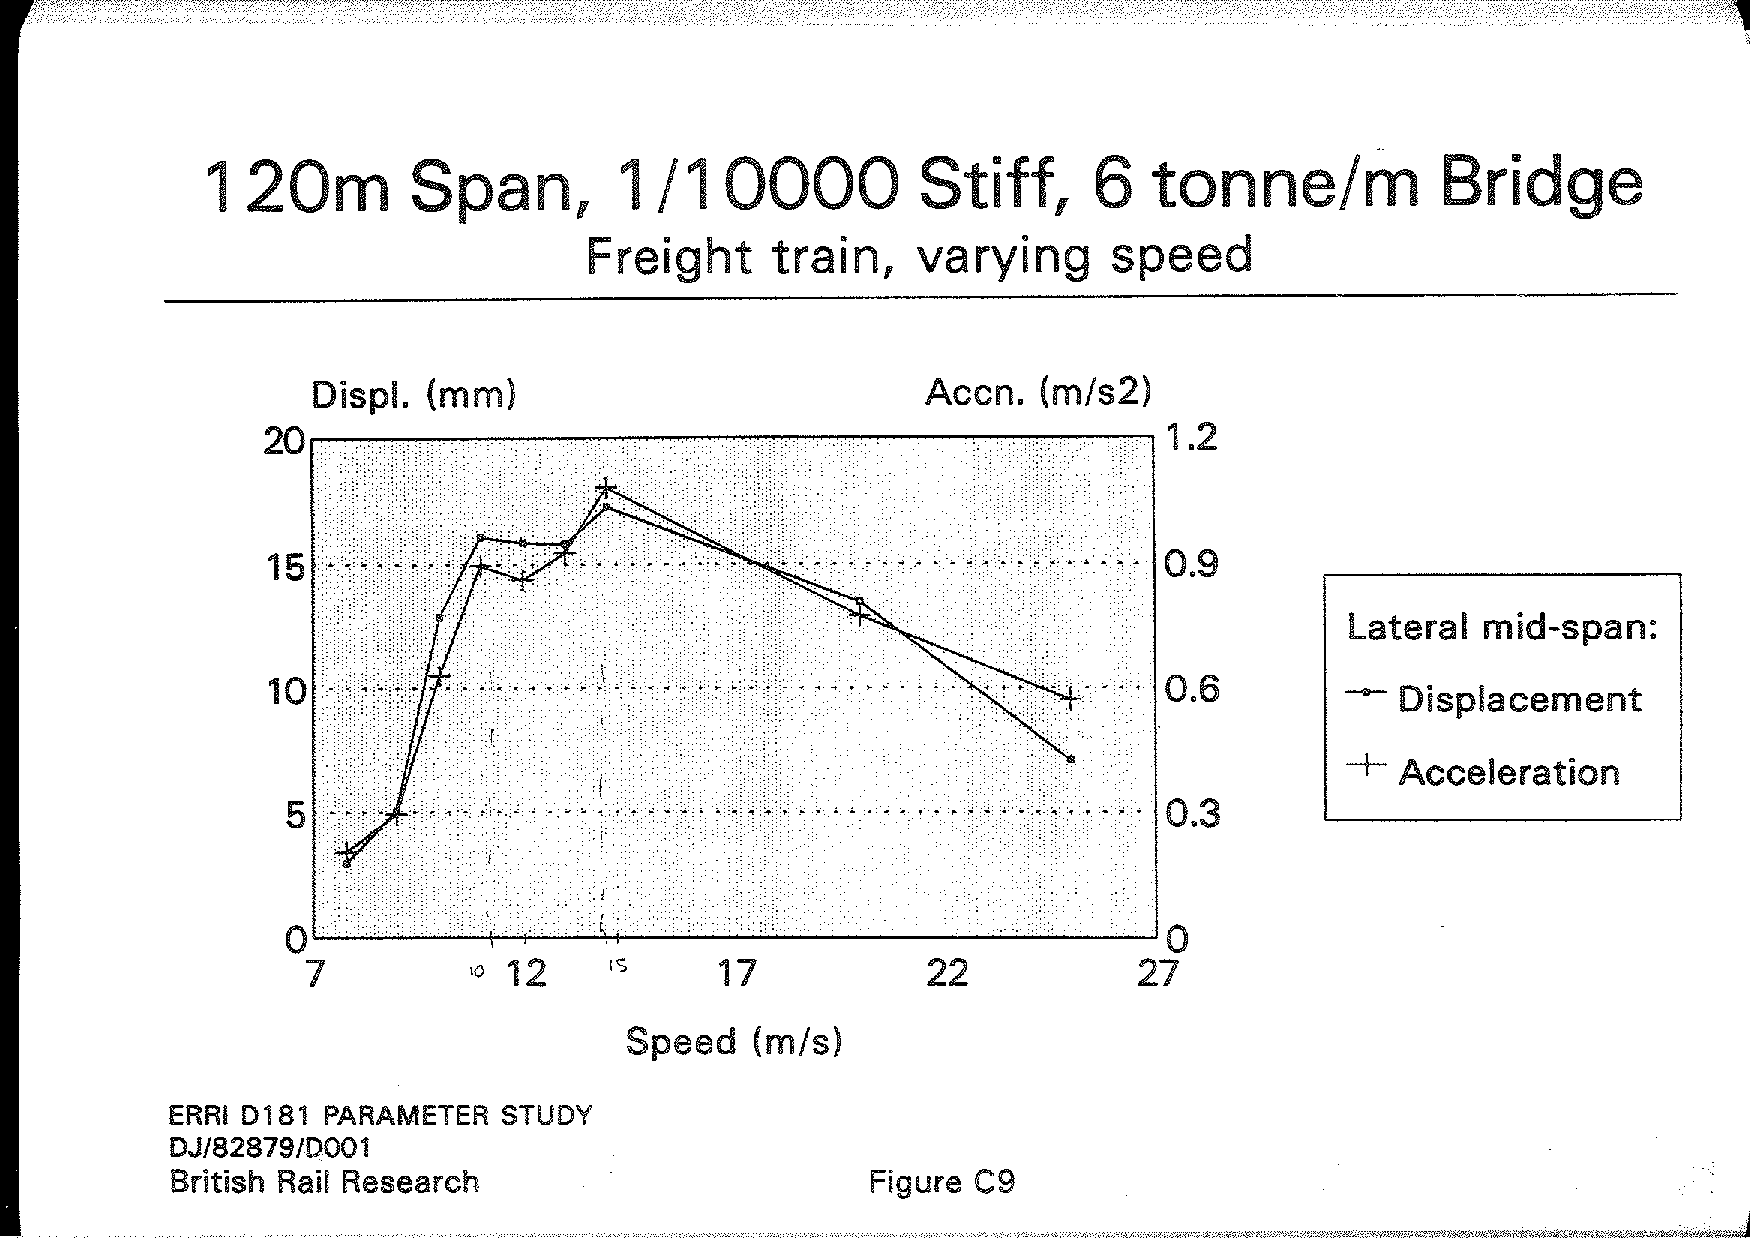
\includegraphics[width=0.8\textwidth]{c9}
    \caption{Figure C3 extracted from \cite{d181dt329} }
    \label{fig:c9}
\end{figure}

The analytical result if presented in Figure.\ref{fig:EJ300000000000L120mu6000c15}.

\begin{figure}[h!]
\centering 
\setlength\figureheight{6cm} 
\setlength\figurewidth{6cm} 
% This file was created by matlab2tikz v0.4.7 (commit d412d9f5e9b0b532484ca0001381d1809ceeed7a) running on MATLAB 8.3.
% Copyright (c) 2008--2014, Nico Schlmer <nico.schloemer@gmail.com>
% All rights reserved.
% Minimal pgfplots version: 1.3
% 
\begin{tikzpicture}

\begin{axis}[%
width=\figurewidth,
height=\figureheight,
scale only axis,
xmin=0,
xmax=8,
ymin=-0.1,
ymax=0.1,
title={Max Deflection:0.00165451876202448,Max Acceleration:0.098608250658388}
]
\addplot [color=blue,solid,forget plot]
  table[row sep=crcr]{%
0	0\\
0.008	7.60734778366103e-06\\
0.016	1.44777344553205e-05\\
0.024	2.06232950239573e-05\\
0.032	2.60597378940296e-05\\
0.04	3.08059863798225e-05\\
0.048	3.48838389133897e-05\\
0.056	3.83176472629258e-05\\
0.064	4.11340120841618e-05\\
0.072	4.33614951358855e-05\\
0.08	4.50303475015986e-05\\
0.088	4.61722531723045e-05\\
0.096	4.68200873601551e-05\\
0.104	4.7007688928906e-05\\
0.112	4.67696463445604e-05\\
0.12	4.61410965680046e-05\\
0.128	4.5157536330612e-05\\
0.136	4.38546452535488e-05\\
0.144	4.22681202916447e-05\\
0.152	4.04335210030608e-05\\
0.16	3.83861251664282e-05\\
0.168	3.61607942875291e-05\\
0.176	3.37918485578188e-05\\
0.184	3.1312950847053e-05\\
0.192	2.87569993318822e-05\\
0.2	2.61560283814414e-05\\
0.208	2.35411173396192e-05\\
0.216	2.09423068617792e-05\\
0.224	1.8388522481185e-05\\
0.232	1.59075050971928e-05\\
0.24	1.35257480934086e-05\\
0.248	1.1268440809417e-05\\
0.256	9.15941810436196e-06\\
0.264	7.22111576458936e-06\\
0.272	5.47453152072655e-06\\
0.28	3.93919145198114e-06\\
0.288	2.63312156708837e-06\\
0.296	1.57282436222749e-06\\
0.304	7.73260166373839e-07\\
0.312	2.47833093965897e-07\\
0.32	8.3814334601738e-09\\
0.328	6.5172308340235e-08\\
0.336	4.26900454458519e-07\\
0.344	1.10069096424307e-06\\
0.352	2.09210585431959e-06\\
0.36	3.40515431850702e-06\\
0.368	5.04230653296924e-06\\
0.376	7.00451088457233e-06\\
0.384	9.29121449723573e-06\\
0.392	1.1900386934304e-05\\
0.4	1.48285469577341e-05\\
0.408	1.80707922272173e-05\\
0.416	2.16208318242721e-05\\
0.424	2.54710214878715e-05\\
0.432	2.96124014493511e-05\\
0.44	3.40347367551931e-05\\
0.448	3.87265599668463e-05\\
0.456	4.36752161270297e-05\\
0.464	4.88669098820232e-05\\
0.472	5.42867546492921e-05\\
0.48	5.99188237194473e-05\\
0.488	6.57462031810458e-05\\
0.496	7.17510465560991e-05\\
0.504	7.79146310334194e-05\\
0.512	8.42174151861016e-05\\
0.52	9.06390980585555e-05\\
0.528	9.71586795075722e-05\\
0.536	0.000103754521680961\\
0.544	0.00011040441151635\\
0.552	0.000117085624141823\\
0.56	0.000123774987059163\\
0.568	0.000130448944989684\\
0.576	0.000137083625261814\\
0.584	0.000143654903619005\\
0.592	0.000150138470325905\\
0.6	0.000156509896450335\\
0.608	0.00016274470019827\\
0.616	0.000168818413178844\\
0.624	0.000174706646476389\\
0.632	0.000180385156406638\\
0.64	0.000185829909834516\\
0.648	0.000191017148931454\\
0.656	0.000195923455250797\\
0.664	0.000200525813000736\\
0.672	0.000204801671395262\\
0.68	0.000208729005964867\\
0.688	0.000212286378710175\\
0.696	0.000215452996983356\\
0.704	0.000218208770984018\\
0.712	0.000220534369758371\\
0.72	0.000222411275592705\\
0.728	0.000223821836694751\\
0.736	0.000224749318059147\\
0.744	0.000225177950416178\\
0.752	0.000225092977166006\\
0.76	0.000224480699203965\\
0.768	0.000223328517545935\\
0.776	0.00022162497366654\\
0.784	0.000219359787466756\\
0.792	0.000216523892791573\\
0.8	0.000213109470422583\\
0.808	0.000209109978474757\\
0.816	0.000204520180131199\\
0.824	0.000199336168654405\\
0.832	0.000193555389617361\\
0.84	0.000187176660302816\\
0.848	0.000180200186224162\\
0.856	0.000172627574726582\\
0.864	0.000164461845632444\\
0.872	0.000155707438900357\\
0.88	0.000146370219272821\\
0.888	0.000136457477892986\\
0.896	0.000125977930876696\\
0.904	0.000114941714831714\\
0.912	0.000103360379321782\\
0.92	9.12468762789393e-05\\
0.928	7.86155463733904e-05\\
0.936	6.54821023559708e-05\\
0.944	5.18636093941472e-05\\
0.952	3.777846242826e-05\\
0.96	2.32463605805312e-05\\
0.968	8.28827865510489e-06\\
0.976	-7.07356422689688e-06\\
0.984	-2.28157388076676e-05\\
0.992	-3.89136426331403e-05\\
1	-5.53415396928168e-05\\
1.008	-7.20726026928646e-05\\
1.016	-8.90789578910293e-05\\
1.024	-0.000106331732416712\\
1.032	-0.000123801103994483\\
1.04	-0.000141456352984358\\
1.048	-0.000159265916647364\\
1.056	-0.000177197445540278\\
1.064	-0.000195217861938922\\
1.072	-0.000213293420185103\\
1.08	-0.000231389768848146\\
1.088	-0.000249472014588022\\
1.096	-0.000267504787603329\\
1.104	-0.000285452308543852\\
1.112	-0.000303278456764089\\
1.12	-0.000320946839791038\\
1.128	-0.000338420863876644\\
1.136	-0.000355663805502673\\
1.144	-0.000372638883703376\\
1.152	-0.000389309333069111\\
1.16	-0.000405638477292239\\
1.168	-0.000421589803114881\\
1.176	-0.000437127034536786\\
1.184	-0.00045221420714037\\
1.192	-0.000466815742389151\\
1.2	-0.000480896521755176\\
1.208	-0.000494421960530704\\
1.216	-0.000507358081179345\\
1.224	-0.000519671586082065\\
1.232	-0.000531329929533929\\
1.24	-0.000542301388848235\\
1.248	-0.000552555134425675\\
1.256	-0.000562061298647496\\
1.264	-0.000570791043453163\\
1.272	-0.000578716626464887\\
1.28	-0.00058581146552345\\
1.288	-0.000592050201502142\\
1.296	-0.000597408759268236\\
1.304	-0.000601864406664282\\
1.312	-0.000605395811384666\\
1.32	-0.000607983095626184\\
1.328	-0.000609607888395072\\
1.336	-0.000610253375356677\\
1.344	-0.000609904346118123\\
1.352	-0.000608547238838532\\
1.36	-0.000606170182065914\\
1.368	-0.000602763033704534\\
1.376	-0.000598317417021462\\
1.384	-0.000592826753606127\\
1.392	-0.000586286293201954\\
1.4	-0.000578693140334621\\
1.408	-0.000570046277667091\\
1.416	-0.00056034658601731\\
1.424	-0.000549596860980404\\
1.432	-0.00053780182610321\\
1.44	-0.000524968142565148\\
1.448	-0.000511104415325713\\
1.456	-0.000496221195705218\\
1.464	-0.000480330980371891\\
1.472	-0.000463448206714924\\
1.48	-0.000445589244589716\\
1.488	-0.000426772384428146\\
1.496	-0.000407017821713433\\
1.504	-0.000386347637825835\\
1.512	-0.000364785777272177\\
1.52	-0.000342358021318929\\
1.528	-0.000319091958055274\\
1.536	-0.00029501694891933\\
1.544	-0.000270164091727314\\
1.552	-0.00024456618025213\\
1.56	-0.000218257660404354\\
1.568	-0.000191274583075149\\
1.576	-0.000163654553707003\\
1.584	-0.000135436678664561\\
1.592	-0.000106661508483972\\
1.6	-7.73709780853272e-05\\
1.608	-4.76083440386846e-05\\
1.616	-1.74181189800418e-05\\
1.624	1.31539967207385e-05\\
1.632	4.40611859325107e-05\\
1.64	7.52555882630694e-05\\
1.648	0.000106688375968983\\
1.656	0.000138309832152045\\
1.664	0.000170069431114601\\
1.672	0.000201915920741425\\
1.68	0.00023379740677156\\
1.688	0.000265661438819341\\
1.696	0.000297455098000061\\
1.704	0.00032912508601206\\
1.712	0.000360617815523661\\
1.72	0.000391879501710323\\
1.728	0.000422856254784471\\
1.736	0.000453494173357974\\
1.744	0.000483739438474904\\
1.752	0.00051353840815024\\
1.76	0.000542837712248437\\
1.768	0.000571584347534401\\
1.776	0.00059972577272822\\
1.784	0.000627210003394253\\
1.792	0.000653985706494561\\
1.8	0.000680002294436527\\
1.808	0.000705210018444501\\
1.816	0.00072956006108579\\
1.824	0.000753004627781887\\
1.832	0.000775497037136948\\
1.84	0.000796991809916704\\
1.848	0.000817444756512716\\
1.856	0.000836813062728671\\
1.864	0.000855055373727711\\
1.872	0.000872131875982221\\
1.88	0.00088800437707034\\
1.888	0.000902636383166487\\
1.896	0.000915993174076619\\
1.904	0.000928041875672514\\
1.912	0.000938751529583348\\
1.92	0.000948093160006969\\
1.928	0.000956039837507751\\
1.936	0.000962566739672579\\
1.944	0.000967651208501498\\
1.952	0.000971272804414687\\
1.96	0.000973413356762893\\
1.968	0.000974057010734044\\
1.976	0.000973190270554631\\
1.984	0.000970802038890499\\
1.992	0.000966883652357903\\
2	0.000961428913062143\\
2.008	0.000954434116087644\\
2.016	0.000945898072870151\\
2.024	0.000935822130388536\\
2.032	0.00092421018612086\\
2.04	0.000911068698716366\\
2.048	0.000896406694342482\\
2.056	0.000880235768673192\\
2.064	0.000862570084492656\\
2.072	0.000843426364895463\\
2.08	0.000822823882072535\\
2.088	0.000800784441679312\\
2.096	0.000777332362790556\\
2.104	0.000752494453453812\\
2.112	0.000726299981861281\\
2.12	0.000698780643167546\\
2.128	0.000669970521988332\\
2.136	0.000639906050623059\\
2.144	0.000608625963051667\\
2.152	0.000576171244763611\\
2.16	0.000542585078484549\\
2.168	0.000507912785873492\\
2.176	0.000472201765270619\\
2.184	0.000435501425583012\\
2.192	0.000397863116402733\\
2.2	0.000359340054458498\\
2.208	0.000319987246509027\\
2.216	0.000279861408792707\\
2.224	0.000239020883154691\\
2.232	0.000197525549978717\\
2.24	0.00015543673805708\\
2.248	0.000112817131537904\\
2.256	6.97306740945953e-05\\
2.264	2.62424704676343e-05\\
2.272	-1.75813144658987e-05\\
2.28	-6.16735589348731e-05\\
2.288	-0.000105966289663802\\
2.296	-0.000150390789240504\\
2.304	-0.000194877705288352\\
2.312	-0.000239357161266036\\
2.32	-0.000283758868714166\\
2.328	-0.000328012240764898\\
2.336	-0.000372046506727818\\
2.344	-0.000415790827562778\\
2.352	-0.000459174412048025\\
2.36	-0.000502126633450116\\
2.368	-0.000544577146500378\\
2.376	-0.000586456004481484\\
2.384	-0.000627693776226648\\
2.392	-0.000668221662833433\\
2.4	-0.000707971613893752\\
2.408	-0.000746876443041835\\
2.416	-0.000784869942622194\\
2.424	-0.00082188699728047\\
2.432	-0.000857863696281035\\
2.44	-0.000892737444356708\\
2.448	-0.000926447070897633\\
2.456	-0.000958932937288533\\
2.464	-0.00099013704220591\\
2.472	-0.00102000312468957\\
2.48	-0.00104847676480591\\
2.488	-0.0010755054817238\\
2.496	-0.00110103882902767\\
2.504	-0.00112502848709641\\
2.512	-0.00114742835238094\\
2.52	-0.00116819462341821\\
2.528	-0.00118728588342406\\
2.536	-0.00120466317931263\\
2.544	-0.0012202900969957\\
2.552	-0.00123413283282092\\
2.56	-0.00124616026101384\\
2.568	-0.00125634399699528\\
2.576	-0.00126465845645157\\
2.584	-0.00127108091004246\\
2.592	-0.00127559153363808\\
2.6	-0.00127817345398356\\
2.608	-0.00127881278969753\\
2.616	-0.00127749868751786\\
2.624	-0.00127422335371606\\
2.632	-0.00126898208060942\\
2.64	-0.00126177326810805\\
2.648	-0.00125259844024212\\
2.656	-0.00124146225662292\\
2.664	-0.0012283725187995\\
2.672	-0.00121334017148154\\
2.68	-0.00119637929860703\\
2.688	-0.00117750711424252\\
2.696	-0.00115674394831195\\
2.704	-0.00113411322715887\\
2.712	-0.00110964144895556\\
2.72	-0.00108335815398125\\
2.728	-0.00105529588980019\\
2.736	-0.00102549017137927\\
2.744	-0.000993979436193011\\
2.752	-0.000960804994372915\\
2.76	-0.000926010973966042\\
2.768	-0.000889644261376495\\
2.776	-0.000851754437071616\\
2.784	-0.000812393706642848\\
2.792	-0.000771616827319385\\
2.8	-0.000729481030040511\\
2.808	-0.000686045937200386\\
2.816	-0.000641373476186521\\
2.824	-0.000595527788840671\\
2.832	-0.000548575136977994\\
2.84	-0.000500583804107371\\
2.848	-0.000451623993502508\\
2.856	-0.000401767722780026\\
2.864	-0.00035108871514695\\
2.872	-0.000299662287486167\\
2.88	-0.000247565235454029\\
2.888	-0.000194875715769939\\
2.896	-0.000141673125882783\\
2.904	-8.80379812041334e-05\\
2.912	-3.40517901026019e-05\\
2.92	2.02030731418527e-05\\
2.928	7.464349722106e-05\\
2.936	0.000129185764312814\\
2.944	0.000183745682016559\\
2.952	0.00023823871649796\\
2.96	0.000292580126627255\\
2.968	0.000346685098893943\\
2.976	0.000400468882878552\\
2.984	0.000453846927060642\\
2.992	0.000506735014741101\\
3	0.000559049399855939\\
3.008	0.000610706942458439\\
3.016	0.000661625243646394\\
3.024	0.000711722779711573\\
3.032	0.000760919035289204\\
3.04	0.000809134635286331\\
3.048	0.000856291475369409\\
3.056	0.00090231285079324\\
3.064	0.000947123583355613\\
3.072	0.000990650146264481\\
3.08	0.00103282078670753\\
3.088	0.0010735656459171\\
3.096	0.00111281687652731\\
3.104	0.0011505087570238\\
3.112	0.0011865778030913\\
3.12	0.00122096287566851\\
3.128	0.00125360528552483\\
3.136	0.00128444889417906\\
3.144	0.00131344021098517\\
3.152	0.00134052848621702\\
3.16	0.00136566579998918\\
3.168	0.00138880714685823\\
3.176	0.00140991051595537\\
3.184	0.00142893696650802\\
3.192	0.00144585069861583\\
3.2	0.00146061911915355\\
3.208	0.00147321290268127\\
3.216	0.00148360604725045\\
3.224	0.00149177592500207\\
3.232	0.00149770332746201\\
3.24	0.00150137250544686\\
3.248	0.00150277120350241\\
3.256	0.00150189068880555\\
3.264	0.00149872577446959\\
3.272	0.00149327483720191\\
3.28	0.00148553982927209\\
3.288	0.00147552628475782\\
3.296	0.00146324332004555\\
3.304	0.00144870362857184\\
3.312	0.00143192346980105\\
3.32	0.00141292265244442\\
3.328	0.00139172451193519\\
3.336	0.00136835588218346\\
3.344	0.00134284706164452\\
3.352	0.00131523177374341\\
3.36	0.00128554712170771\\
3.368	0.00125383353787036\\
3.376	0.00122013472751299\\
3.384	0.00118449760732948\\
3.392	0.0011469722385987\\
3.4	0.00110761175516391\\
3.408	0.00106647228632504\\
3.416	0.00102361287475898\\
3.424	0.000979095389590702\\
3.432	0.000932984434747002\\
3.44	0.000885347252731921\\
3.448	0.000836253623971142\\
3.456	0.0007857757618799\\
3.464	0.000733988203816412\\
3.472	0.000680967698089717\\
3.48	0.000626793087197683\\
3.488	0.000571545187477288\\
3.496	0.000515306665355641\\
3.504	0.000458161910395931\\
3.512	0.000400196905338174\\
3.52	0.000341499093339777\\
3.528	0.000282157242625998\\
3.536	0.000222261308764853\\
3.544	0.000161902294785226\\
3.552	0.000101172109360984\\
3.56	4.01634232872216e-05\\
3.568	-2.10304755219463e-05\\
3.576	-8.23158282819925e-05\\
3.584	-0.000143598552598348\\
3.592	-0.000204784390502087\\
3.6	-0.000265779057022684\\
3.608	-0.000326488389058557\\
3.616	-0.000386818494305011\\
3.624	-0.000446675899999021\\
3.632	-0.00050596770124003\\
3.64	-0.000564601708646479\\
3.648	-0.000622486595108299\\
3.656	-0.000679532041396972\\
3.664	-0.000735648880396103\\
3.672	-0.000790749239717572\\
3.68	-0.000844746682470411\\
3.688	-0.000897556345952485\\
3.696	-0.00094909507803797\\
3.704	-0.000999281571037237\\
3.712	-0.00104803649280939\\
3.72	-0.00109528261491211\\
3.728	-0.00114094493757786\\
3.736	-0.00118495081131058\\
3.744	-0.00122723005490199\\
3.752	-0.00126771506967257\\
3.76	-0.00130634094974789\\
3.768	-0.00134304558818741\\
3.776	-0.00137776977878928\\
3.784	-0.00141045731340156\\
3.792	-0.00144105507457754\\
3.8	-0.00146951312341994\\
3.808	-0.00149578478246676\\
3.816	-0.00151982671347928\\
3.824	-0.00154159899000086\\
3.832	-0.00156106516456376\\
3.84	-0.00157819233042942\\
3.848	-0.00159295117775687\\
3.856	-0.00160531604410256\\
3.864	-0.00161526495916416\\
3.872	-0.0016227796836902\\
3.88	-0.00162784574248683\\
3.888	-0.00163045245146232\\
3.896	-0.00163059293866002\\
3.904	-0.00162826415923971\\
3.912	-0.00162346690437746\\
3.92	-0.00161620580406383\\
3.928	-0.00160648932379016\\
3.936	-0.00159432975512271\\
3.944	-0.0015797432001742\\
3.952	-0.00156274954999247\\
3.96	-0.00154337245689556\\
3.968	-0.0015216393007928\\
3.976	-0.00149758114954089\\
3.984	-0.00147123271339393\\
3.992	-0.00144263229361609\\
4	-0.00141182172533477\\
4.008	-0.00137884631472203\\
4.016	-0.00134375477060086\\
4.024	-0.00130659913058246\\
4.032	-0.00126743468184919\\
4.04	-0.00122631987670704\\
4.048	-0.0011833162430398\\
4.056	-0.00113848828980552\\
4.064	-0.00109190340772417\\
4.072	-0.00104363176531298\\
4.08	-0.000993746200433931\\
4.088	-0.000942322107525082\\
4.096	-0.000889437320694479\\
4.104	-0.000835171992862378\\
4.112	-0.00077960847114388\\
4.12	-0.000722831168670381\\
4.128	-0.00066492643305401\\
4.136	-0.000605982411704961\\
4.144	-0.00054608891421662\\
4.152	-0.000485337272038442\\
4.16	-0.000423820195660846\\
4.168	-0.000361631629540743\\
4.176	-0.000298866604999835\\
4.184	-0.000235621091331527\\
4.192	-0.000171991845354763\\
4.2	-0.000108076259656475\\
4.208	-4.39722097656531e-05\\
4.216	2.02220994952293e-05\\
4.224	8.44082882352328e-05\\
4.232	0.000148487956048202\\
4.24	0.000212362836646419\\
4.248	0.000275934952325713\\
4.256	0.000339106768014205\\
4.264	0.000401781344656516\\
4.272	0.000463862491687263\\
4.28	0.000525254918348173\\
4.288	0.000585864383605881\\
4.296	0.000645597844428776\\
4.304	0.00070436360218479\\
4.312	0.000762071446924193\\
4.32	0.000818632799315714\\
4.328	0.000873960850007166\\
4.336	0.000927970696186847\\
4.344	0.000980579475125636\\
4.352	0.00103170649448543\\
4.36	0.00108127335918393\\
4.368	0.00112920409461231\\
4.376	0.00117542526600714\\
4.384	0.00121986609378546\\
4.392	0.001262458564657\\
4.4	0.0013031375383358\\
4.408	0.00134184084967951\\
4.416	0.00137850940609288\\
4.424	0.00141308728003908\\
4.432	0.00144552179651085\\
4.44	0.00147576361532132\\
4.448	0.00150376680808322\\
4.456	0.00152948892975323\\
4.464	0.00155289108462771\\
4.472	0.00157393798668443\\
4.48	0.00159259801417483\\
4.488	0.00160884325837986\\
4.496	0.00162264956645276\\
4.504	0.00163399657828107\\
4.512	0.00164286775731045\\
4.52	0.00164925041528221\\
4.528	0.00165313573084671\\
4.536	0.00165451876202448\\
4.544	0.00165339845249724\\
4.552	0.0016497776317205\\
4.56	0.00164366300885999\\
4.568	0.00163506516056389\\
4.576	0.00162399851259287\\
4.584	0.00161048131533994\\
4.592	0.00159453561328209\\
4.6	0.00157618720841541\\
4.608	0.00155546561773513\\
4.616	0.00153240402483184\\
4.624	0.00150703922568438\\
4.632	0.00147941156873966\\
4.64	0.00144956488937834\\
4.648	0.0014175464388751\\
4.656	0.00138340680797036\\
4.664	0.00134719984517969\\
4.672	0.0013089825699749\\
4.68	0.00126881508097993\\
4.688	0.00122676045933172\\
4.696	0.00118288466736481\\
4.704	0.00113725644278547\\
4.712	0.0010899471885084\\
4.72	0.00104103085833636\\
4.728	0.000990583838669061\\
4.736	0.000938684826434739\\
4.744	0.000885414703443156\\
4.752	0.000830856407364963\\
4.76	0.000775094799547339\\
4.768	0.000718216529881064\\
4.776	0.000660309898938628\\
4.784	0.000601464717607406\\
4.792	0.000541772164445638\\
4.8	0.000481324640992728\\
4.808	0.000420215625268254\\
4.816	0.000358539523697057\\
4.824	0.000296391521699934\\
4.832	0.000233867433191638\\
4.84	0.000171063549229291\\
4.848	0.000108076486055581\\
4.856	4.50030327817846e-05\\
4.864	-1.80600010438144e-05\\
4.872	-8.10159377367698e-05\\
4.88	-0.000143768383401517\\
4.888	-0.000206221379236569\\
4.896	-0.000268279551976831\\
4.904	-0.000329848263231889\\
4.912	-0.00039083375748094\\
4.92	-0.000451143308487682\\
4.928	-0.000510685363901053\\
4.936	-0.0005693696878111\\
4.944	-0.00062710750103271\\
4.952	-0.000683811618893987\\
4.96	-0.000739396586310194\\
4.968	-0.000793778809929015\\
4.976	-0.000846876687137764\\
4.984	-0.000898610731728641\\
4.992	-0.000948903696023634\\
5	-0.000997680689266848\\
5.008	-0.00104486929209819\\
5.016	-0.00109039966692906\\
5.024	-0.00113420466404756\\
5.032	-0.0011762199232877\\
5.04	-0.00121638397110495\\
5.048	-0.00125463831290773\\
5.056	-0.00129092752050247\\
5.064	-0.00132519931451828\\
5.072	-0.00135740464168518\\
5.08	-0.00138749774684878\\
5.088	-0.00141543623961277\\
5.096	-0.00144118115550968\\
5.104	-0.00146469701160922\\
5.112	-0.00148595185648297\\
5.12	-0.00150491731445315\\
5.128	-0.00152156862406301\\
5.136	-0.00153588467071554\\
5.144	-0.0015478480134371\\
5.152	-0.00155744490573195\\
5.16	-0.00156466531050347\\
5.168	-0.00156950290902767\\
5.176	-0.00157195510397412\\
5.184	-0.00157202301647924\\
5.192	-0.0015697114772867\\
5.2	-0.00156502901197912\\
5.208	-0.00155798782033505\\
5.216	-0.00154860374985467\\
5.224	-0.00153689626350711\\
5.232	-0.0015228884017617\\
5.24	-0.00150660673897448\\
5.248	-0.00148808133421083\\
5.256	-0.00146734567659349\\
5.264	-0.00144443662527453\\
5.272	-0.00141939434413813\\
5.28	-0.00139226223134963\\
5.288	-0.00136308684387432\\
5.296	-0.00133191781709791\\
5.304	-0.00129880777968772\\
5.312	-0.00126381226384185\\
5.32	-0.00122698961108032\\
5.328	-0.00118840087373967\\
5.336	-0.00114810971233868\\
5.344	-0.00110618228899006\\
5.352	-0.00106268715703822\\
5.36	-0.00101769514710998\\
5.368	-0.00097127924976984\\
5.376	-0.000923514494977147\\
5.384	-0.000874477828547017\\
5.392	-0.000824247985821721\\
5.4	-0.000772905362762969\\
5.408	-0.000720531884679905\\
5.416	-0.000667210872810419\\
5.424	-0.000613026908977186\\
5.432	-0.00055806569854183\\
5.44	-0.000502413931883663\\
5.448	-0.000446159144630664\\
5.456	-0.000389389576872737\\
5.464	-0.00033219403158769\\
5.472	-0.00027466173251195\\
5.48	-0.000216882181687667\\
5.488	-0.000158945016918749\\
5.496	-0.000100939869367171\\
5.504	-4.29562215209949e-05\\
5.512	1.49167342364137e-05\\
5.52	7.25902362270715e-05\\
5.528	0.000129976093022836\\
5.536	0.000186986821708893\\
5.544	0.00024353578464496\\
5.552	0.000299537324505013\\
5.56	0.000354906897380498\\
5.568	0.000409561203734882\\
5.576	0.000463418317002195\\
5.584	0.000516397809625755\\
5.592	0.000568420876338754\\
5.6	0.000619410454492638\\
5.608	0.000669291341245279\\
5.616	0.000717990307425753\\
5.624	0.000765436207899251\\
5.632	0.000811560088261087\\
5.64	0.000856295287695965\\
5.648	0.000899577537844618\\
5.656	0.000941345057527663\\
5.664	0.000981538643183011\\
5.672	0.00102010175488125\\
5.68	0.00105698059779043\\
5.688	0.00109212419897009\\
5.696	0.00112548447938182\\
5.704	0.00115701632101242\\
5.712	0.00118667762901348\\
5.72	0.00121442938877015\\
5.728	0.00124023571782006\\
5.736	0.00126406391255261\\
5.744	0.0012858844896269\\
5.752	0.00130567122205632\\
5.76	0.00132340116991601\\
5.768	0.00133905470563896\\
5.776	0.00135261553387526\\
5.784	0.0013640707058982\\
5.792	0.00137341062854998\\
5.8	0.00138062906772871\\
5.808	0.00138572314642782\\
5.816	0.0013886933373473\\
5.824	0.00138954345010599\\
5.832	0.00138828061309215\\
5.84	0.00138491524999905\\
5.848	0.0013794610511005\\
5.856	0.00137193493933003\\
5.864	0.00136235703123593\\
5.872	0.00135075059289242\\
5.88	0.00133714199085558\\
5.888	0.00132156063826055\\
5.896	0.0013040389361644\\
5.904	0.00128461221024635\\
5.912	0.00126331864298487\\
5.92	0.00124019920143806\\
5.928	0.00121529756076056\\
5.936	0.00118866002359725\\
5.944	0.00116033543550019\\
5.952	0.0011303750965215\\
5.96	0.00109883266914079\\
5.968	0.00106576408269127\\
5.976	0.00103122743445429\\
5.984	0.000995282887596664\\
5.992	0.000957992566130181\\
6	0.000919420447076965\\
6.008	0.000879632250028484\\
6.016	0.000838695324289734\\
6.024	0.000796678533803506\\
6.032	0.000753652140052848\\
6.04	0.000709687683142465\\
6.048	0.000664857861262194\\
6.056	0.000619236408737841\\
6.064	0.000572897972876229\\
6.072	0.00052591798981276\\
6.08	0.000478372559570648\\
6.088	0.000430338320541758\\
6.096	0.000381892323599124\\
6.104	0.000333111906051234\\
6.112	0.000284074565647605\\
6.12	0.00023485783484455\\
6.128	0.000185539155538726\\
6.136	0.000136195754474688\\
6.144	8.69045195306957e-05\\
6.152	3.77418770850381e-05\\
6.16	-1.12163293375782e-05\\
6.168	-5.98949589427147e-05\\
6.176	-0.000108219691872411\\
6.184	-0.00015611714555069\\
6.192	-0.000203514988982096\\
6.2	-0.000250342054820967\\
6.208	-0.000296528449033696\\
6.216	-0.000342005657980727\\
6.224	-0.000386706652750202\\
6.232	-0.000430565990580247\\
6.24	-0.000473519913212543\\
6.248	-0.000515506442025403\\
6.256	-0.000556465469800708\\
6.264	-0.000596338848985194\\
6.272	-0.000635070476313078\\
6.28	-0.000672606373663557\\
6.288	-0.000708894765033655\\
6.296	-0.000743886149513823\\
6.304	-0.000777533370160977\\
6.312	-0.000809791678670863\\
6.32	-0.000840618795759277\\
6.328	-0.000869974967169143\\
6.336	-0.000897823015228317\\
6.344	-0.000924128385890671\\
6.352	-0.000948859191201085\\
6.36	-0.000971986247132803\\
6.368	-0.000993483106753895\\
6.376	-0.00101332608868738\\
6.384	-0.00103149430083799\\
6.392	-0.00104796965936652\\
6.4	-0.00106273690290092\\
6.408	-0.00107578360198149\\
6.416	-0.00108710016374563\\
6.424	-0.00109667983186556\\
6.432	-0.00110451868176082\\
6.44	-0.00111061561111485\\
6.448	-0.00111497232573326\\
6.456	-0.00111759332078897\\
6.464	-0.0011184858575072\\
6.472	-0.00111765993535076\\
6.48	-0.00111512825977375\\
6.488	-0.0011109062056188\\
6.496	-0.00110501177624034\\
6.504	-0.00109746555844335\\
6.512	-0.00108829067333373\\
6.52	-0.00107751272318309\\
6.528	-0.00106515973441727\\
6.536	-0.001051262096844\\
6.544	-0.00103585249924096\\
6.552	-0.00101896586143163\\
6.56	-0.00100063926298129\\
6.568	-0.000980911868651371\\
6.576	-0.000959824850754696\\
6.584	-0.000937421308559612\\
6.592	-0.000913746184894739\\
6.6	-0.000888846180110829\\
6.608	-0.000862769663559709\\
6.616	-0.000835566582754138\\
6.624	-0.000807288370375542\\
6.632	-0.000777987849299656\\
6.64	-0.00074771913581277\\
6.648	-0.000716537541193697\\
6.656	-0.000684499471838518\\
6.664	-0.000651662328107086\\
6.672	-0.00061808440207152\\
6.68	-0.000583824774348122\\
6.688	-0.000548943210194977\\
6.696	-0.000513500055057812\\
6.704	-0.000477556129746955\\
6.712	-0.000441172625428087\\
6.72	-0.000404410998608815\\
6.728	-0.000367332866302434\\
6.736	-0.000329999901549138\\
6.744	-0.000292473729473278\\
6.752	-0.000254815824053859\\
6.76	-0.000217087405783079\\
6.768	-0.000179349340385566\\
6.776	-0.000141662038768355\\
6.784	-0.000104085358368492\\
6.792	-6.66785060621497e-05\\
6.8	-2.94999427956461e-05\\
6.808	7.39270990524821e-06\\
6.816	4.39427613949609e-05\\
6.824	8.00945411886326e-05\\
6.832	0.000115793485919674\\
6.84	0.000150986223835313\\
6.848	0.000185620656696234\\
6.856	0.00021964603895143\\
6.864	0.000253013054064803\\
6.872	0.000285673887875848\\
6.88	0.00031758229888222\\
6.888	0.000348693685338284\\
6.896	0.000378965149069648\\
6.904	0.000408355555909985\\
6.912	0.000436825592673028\\
6.92	0.000464337820578995\\
6.928	0.000490856725061396\\
6.936	0.00051634876188712\\
6.944	0.000540782399529275\\
6.952	0.000564128157739481\\
6.96	0.000586358642273166\\
6.968	0.000607448575728462\\
6.976	0.00062737482446657\\
6.984	0.000646116421588436\\
6.992	0.00066365458594976\\
7	0.00067997273720365\\
7.008	0.000695056506867158\\
7.016	0.000708893745415283\\
7.024	0.000721474525412959\\
7.032	0.000732791140702621\\
7.04	0.000742838101672004\\
7.048	0.000751612126633621\\
7.056	0.000759112129354261\\
7.064	0.000765339202779556\\
7.072	0.000770296599005305\\
7.08	0.000773989705553665\\
7.088	0.000776426018018828\\
7.096	0.000777615109152843\\
7.104	0.000777568594468493\\
7.112	0.000776300094441929\\
7.12	0.000773825193403506\\
7.128	0.000770161395210903\\
7.136	0.00076532807580384\\
7.144	0.00075934643274498\\
7.152	0.00075223943185645\\
7.16	0.000744031751066232\\
7.168	0.000734749721583085\\
7.176	0.000724421266523007\\
7.184	0.000713075837114217\\
7.192	0.000700744346611431\\
7.2	0.000687459102053734\\
7.208	0.00067325373400362\\
7.216	0.000658163124407751\\
7.224	0.000642223332722748\\
7.232	0.000625471520451761\\
7.24	0.000607945874239748\\
7.248	0.000589685527677353\\
7.256	0.000570730481964794\\
7.264	0.000551121525588581\\
7.272	0.000530900153164976\\
7.28	0.000510108483604711\\
7.288	0.00048878917775419\\
7.296	0.000466985355668368\\
7.304	0.000444740513670554\\
7.312	0.000422098441353982\\
7.32	0.000399103138679259\\
7.328	0.000375798733320918\\
7.336	0.000352229398415126\\
7.344	0.000328439270858938\\
7.352	0.000304472370309925\\
7.36	0.000280372519032791\\
7.368	0.000256183262737376\\
7.376	0.000231947792549915\\
7.384	0.000207708868256502\\
7.392	0.000183508742954729\\
7.4	0.000159389089246211\\
7.408	0.000135390927099028\\
7.416	0.000111554553505499\\
7.424	8.79194740566926e-05\\
7.432	6.45243365507985e-05\\
7.44	4.14068667482679e-05\\
7.448	1.86038063818324e-05\\
7.456	-3.84914647501429e-06\\
7.464	-2.59173945826924e-05\\
7.472	-4.75674961598045e-05\\
7.48	-6.87672168690429e-05\\
7.488	-8.94855790817858e-05\\
7.496	-0.000109692908344375\\
7.504	-0.000129360876974393\\
7.512	-0.000148462544721313\\
7.52	-0.000166972396431535\\
7.528	-0.000184866376664006\\
7.536	-0.000202121921208489\\
7.544	-0.0002187179854648\\
7.552	-0.000234635069647447\\
7.56	-0.00024985524078627\\
7.568	-0.000264362151500086\\
7.576	-0.000278141055526415\\
7.584	-0.000291178819996814\\
7.592	-0.000303463934453541\\
7.6	-0.000314986516609506\\
7.608	-0.000325738314859795\\
7.616	-0.000335712707559192\\
7.624	-0.000344904699086233\\
7.632	-0.000353310912720545\\
7.64	-0.000360929580366083\\
7.648	-0.00036776052915894\\
7.656	-0.000373805165004186\\
7.664	-0.000379066453091899\\
7.672	-0.000383548895448262\\
7.68	-0.000387258505583008\\
7.688	-0.000390202780299883\\
7.696	-0.00039239066874204\\
7.704	-0.000393832538749298\\
7.712	-0.000394540140609099\\
7.72	-0.000394526568287754\\
7.728	-0.000393806218233066\\
7.736	-0.000392394745843801\\
7.744	-0.000390309019705624\\
7.752	-0.000387567073697065\\
7.76	-0.000384188057072821\\
7.768	-0.000380192182635242\\
7.776	-0.000375600673108095\\
7.784	-0.000370435705829845\\
7.792	-0.000364720355886448\\
7.8	-0.000358478537806295\\
7.808	-0.000351734945942288\\
7.816	-0.000344514993668092\\
7.824	-0.000336844751517527\\
7.832	-0.000328750884397569\\
7.84	-0.000320260588006871\\
7.848	-0.000311401524592674\\
7.856	-0.000302201758179933\\
7.864	-0.000292689689406894\\
7.872	-0.000282893990101781\\
7.88	-0.000272843537735215\\
7.888	-0.00026256734988275\\
7.896	-0.000252094518831478\\
7.904	-0.000241454146463866\\
7.912	-0.000230675279550969\\
7.92	-0.000219786845585959\\
7.928	-0.000208817589287335\\
7.936	-0.000197796009899458\\
7.944	-0.000186750299416048\\
7.952	-0.000175708281850014\\
7.96	-0.000164697353670512\\
7.968	-0.000153744425525454\\
7.976	-0.000142875865364673\\
7.984	-0.000132117443075896\\
7.992	-0.000121494276742213\\
8	-0.000111030780626223\\
};
\addplot [color=black!50!green,solid,forget plot]
  table[row sep=crcr]{%
0	-0.0116485478509245\\
0.008	-0.0109567760626958\\
0.016	-0.0102043858163887\\
0.024	-0.0093987051361471\\
0.032	-0.00854675413134631\\
0.04	-0.00765525266870444\\
0.048	-0.00673062801908302\\
0.056	-0.00577902243584872\\
0.064	-0.00480630062769537\\
0.072	-0.00381805709439415\\
0.08	-0.00281962329907231\\
0.088	-0.00181607465533936\\
0.096	-0.000812237311904338\\
0.104	0.000187305278719776\\
0.112	0.00117820601722899\\
0.12	0.00215634804679673\\
0.128	0.00311783887818425\\
0.136	0.00405900475162388\\
0.144	0.00497638523402952\\
0.152	0.00586672804797381\\
0.16	0.00672698412700219\\
0.168	0.00755430289021503\\
0.176	0.0083460277276247\\
0.184	0.00909969168657097\\
0.192	0.00981301334844158\\
0.2	0.0104838928840821\\
0.208	0.0111104082755779\\
0.216	0.0116908116915391\\
0.224	0.0122235260026051\\
0.232	0.0127071414235997\\
0.24	0.013140412268597\\
0.248	0.0135222538050977\\
0.256	0.0138517391935489\\
0.264	0.0141280964985701\\
0.272	0.0143507057584495\\
0.28	0.0145190960997599\\
0.288	0.0146329428842848\\
0.296	0.0146920648758564\\
0.304	0.0146964214151588\\
0.312	0.0146461095910593\\
0.32	0.0145413613975748\\
0.328	0.0143825408661583\\
0.336	0.0141701411636071\\
0.344	0.013904781646525\\
0.352	0.013587204863933\\
0.36	0.0132182735002968\\
0.368	0.0127989672519249\\
0.376	0.012330379630393\\
0.384	0.0118137146873502\\
0.392	0.0112502836557709\\
0.4	0.0106415015034231\\
0.408	0.00998888339502678\\
0.416	0.00929404106027754\\
0.424	0.00855867906559882\\
0.432	0.00778459098817155\\
0.44	0.00697365549145876\\
0.448	0.00612783230210035\\
0.456	0.00524915808869604\\
0.464	0.00433974224361996\\
0.472	0.00340176256961837\\
0.48	0.00243746087353106\\
0.488	0.00144913847004532\\
0.496	0.000439151598938977\\
0.504	-0.000590093240206485\\
0.512	-0.00163614403133901\\
0.52	-0.00269650805835399\\
0.528	-0.00376865678918172\\
0.536	-0.00485003082170011\\
0.544	-0.00593804488522527\\
0.552	-0.00703009289095479\\
0.56	-0.00812355302438759\\
0.568	-0.00921579287241902\\
0.576	-0.010304174577512\\
0.584	-0.0113860600110736\\
0.592	-0.0124588159579213\\
0.6	-0.0135198193035067\\
0.608	-0.0145664622153727\\
0.616	-0.0155961573101566\\
0.624	-0.0166063427973137\\
0.632	-0.0175944875906269\\
0.64	-0.01855809637848\\
0.648	-0.0194947146438179\\
0.656	-0.0204019336246799\\
0.664	-0.0212773952061881\\
0.672	-0.0221187967348888\\
0.68	-0.0229238957463865\\
0.688	-0.0236905145972778\\
0.696	-0.0244165449924802\\
0.704	-0.0250999523991664\\
0.712	-0.0257387803386475\\
0.72	-0.0263311545477078\\
0.728	-0.0268752870010725\\
0.736	-0.0273694797868891\\
0.744	-0.0278121288273232\\
0.752	-0.0282017274366084\\
0.76	-0.0285368697091503\\
0.768	-0.0288162537305562\\
0.776	-0.0290386846047609\\
0.784	-0.0292030772907241\\
0.792	-0.0293084592425048\\
0.8	-0.0293539728468551\\
0.808	-0.029338877652832\\
0.816	-0.0292625523882961\\
0.824	-0.0291244967585404\\
0.832	-0.0289243330226929\\
0.84	-0.0286618073439304\\
0.848	-0.0283367909099613\\
0.856	-0.0279492808206507\\
0.864	-0.0274994007400944\\
0.872	-0.0269874013108828\\
0.88	-0.0264136603287398\\
0.888	-0.0257786826761681\\
0.896	-0.0250831000141868\\
0.904	-0.0243276702317016\\
0.912	-0.0235132766525058\\
0.92	-0.0226409270003715\\
0.928	-0.0217117521231504\\
0.936	-0.0207270044772629\\
0.944	-0.019688056374414\\
0.952	-0.0185963979928328\\
0.96	-0.0174536351557823\\
0.968	-0.016261486880542\\
0.976	-0.0150217827015054\\
0.984	-0.0137364597714788\\
0.992	-0.0124075597456973\\
1	-0.0110372254535029\\
1.008	-0.00962769736304452\\
1.016	-0.0081813098447705\\
1.024	-0.00670048723988196\\
1.032	-0.00518773974030424\\
1.04	-0.00364565908711054\\
1.048	-0.00207691409469708\\
1.056	-0.00048424600836138\\
1.064	0.00112953629672569\\
1.072	0.00276156126683873\\
1.08	0.00440889976268186\\
1.088	0.00606857028511748\\
1.096	0.0077375443244404\\
1.104	0.00941275182373532\\
1.112	0.01109108674661\\
1.12	0.0127694127393683\\
1.128	0.0144445688774777\\
1.136	0.0161133754859922\\
1.144	0.0177726400234203\\
1.152	0.0194191630183724\\
1.16	0.0210497440481867\\
1.168	0.0226611877486188\\
1.176	0.0242503098435843\\
1.184	0.0258139431838673\\
1.192	0.0273489437836553\\
1.2	0.0288521968437243\\
1.208	0.0303206227500853\\
1.216	0.0317511830369093\\
1.224	0.0331408863025757\\
1.232	0.0344867940677374\\
1.24	0.0357860265643618\\
1.248	0.0370357684448005\\
1.256	0.0382332744000452\\
1.264	0.0393758746764586\\
1.272	0.0404609804804207\\
1.28	0.0414860892604964\\
1.288	0.0424487898569217\\
1.296	0.0433467675084128\\
1.304	0.0441778087065312\\
1.312	0.0449398058880781\\
1.32	0.045630761956263\\
1.328	0.0462487946216633\\
1.336	0.0467921405542981\\
1.344	0.0472591593384485\\
1.352	0.0476483372221909\\
1.36	0.0479582906539545\\
1.368	0.0481877695987776\\
1.376	0.0483356606273121\\
1.384	0.0484009897710136\\
1.392	0.0483829251373612\\
1.4	0.0482807792793616\\
1.408	0.0480940113140208\\
1.416	0.0478222287849044\\
1.424	0.0474651892643534\\
1.432	0.0470228016913799\\
1.44	0.0464951274417325\\
1.448	0.0458823811270932\\
1.456	0.0451849311208483\\
1.464	0.0444032998083606\\
1.472	0.0435381635601609\\
1.48	0.0425903524269728\\
1.488	0.0415608495559821\\
1.496	0.040450790328263\\
1.504	0.0392614612177774\\
1.512	0.0379942983728627\\
1.52	0.0366508859216322\\
1.528	0.0352329540032084\\
1.536	0.033742376527212\\
1.544	0.0321811686644268\\
1.552	0.0305514840720508\\
1.56	0.0288556118574355\\
1.568	0.0270959732846948\\
1.576	0.0252751182290437\\
1.584	0.0233957213841933\\
1.592	0.0214605782285915\\
1.6	0.0194726007567487\\
1.608	0.0174348129823296\\
1.616	0.0153503462201236\\
1.624	0.0132224341544258\\
1.632	0.0110544077017666\\
1.64	0.00884968967632365\\
1.648	0.00661178926672884\\
1.656	0.00434429633334967\\
1.664	0.00205087553547474\\
1.672	-0.000264739701831562\\
1.68	-0.00259875337112296\\
1.688	-0.00494731320582791\\
1.696	-0.00730651713270117\\
1.704	-0.00967241984253765\\
1.712	-0.0120410394679653\\
1.72	-0.0144083643569117\\
1.728	-0.0167703599301247\\
1.736	-0.0191229756109465\\
1.744	-0.0214621518153643\\
1.752	-0.0237838269902248\\
1.76	-0.0260839446873614\\
1.768	-0.0283584606612924\\
1.776	-0.0306033499780514\\
1.784	-0.0328146141226644\\
1.792	-0.0349882880927361\\
1.8	-0.0371204474656018\\
1.808	-0.0392072154264981\\
1.816	-0.0412447697452399\\
1.824	-0.0432293496889339\\
1.832	-0.0451572628583387\\
1.84	-0.0470248919355668\\
1.848	-0.0488287013309475\\
1.856	-0.0505652437170014\\
1.864	-0.0522311664376404\\
1.872	-0.0538232177808864\\
1.88	-0.0553382531036028\\
1.888	-0.0567732407969574\\
1.896	-0.0581252680815786\\
1.904	-0.0593915466216262\\
1.912	-0.0605694179472885\\
1.92	-0.0616563586755105\\
1.928	-0.062649985519087\\
1.936	-0.0635480600745885\\
1.944	-0.0643484933799471\\
1.952	-0.0650493502329022\\
1.96	-0.0656488532618967\\
1.968	-0.0661453867414216\\
1.976	-0.066537500144226\\
1.984	-0.0668239114232474\\
1.992	-0.0670035100165657\\
2	-0.0670753595691467\\
2.008	-0.0670387003656161\\
2.016	-0.0668929514687904\\
2.024	-0.0666377125591868\\
2.032	-0.0662727654712437\\
2.04	-0.0657980754224931\\
2.048	-0.0652137919324544\\
2.056	-0.0645202494285453\\
2.064	-0.0637179675368438\\
2.072	-0.0628076510560757\\
2.08	-0.0617901896137472\\
2.088	-0.0606666570038928\\
2.096	-0.0594383102064579\\
2.104	-0.058106588088889\\
2.112	-0.0566731097910587\\
2.12	-0.0551396727952035\\
2.128	-0.053508250683105\\
2.136	-0.0517809905832915\\
2.144	-0.0499602103115877\\
2.152	-0.0480483952088727\\
2.16	-0.046048194680451\\
2.168	-0.043962418441964\\
2.176	-0.0417940324772954\\
2.184	-0.0395461547144349\\
2.192	-0.0372220504257747\\
2.2	-0.0348251273598003\\
2.208	-0.0323589306116306\\
2.216	-0.0298271372403267\\
2.224	-0.027233550641355\\
2.232	-0.0245820946830317\\
2.24	-0.0218768076162139\\
2.248	-0.0191218357669124\\
2.256	-0.0163214270219134\\
2.264	-0.0134799241178693\\
2.272	-0.0106017577447\\
2.28	-0.00769143947448451\\
2.288	-0.00475355452736459\\
2.296	-0.0017927543862866\\
2.304	0.00118625072729097\\
2.312	0.00417869950433222\\
2.32	0.00717978731314891\\
2.328	0.0101846740654384\\
2.336	0.0131884921703442\\
2.344	0.0161863545632652\\
2.352	0.0191733627959689\\
2.36	0.0221446151744301\\
2.368	0.025095214930688\\
2.376	0.0280202784149291\\
2.384	0.0309149432939205\\
2.392	0.0337743767418808\\
2.4	0.0365937836098391\\
2.408	0.0393684145595455\\
2.416	0.0420935741480054\\
2.424	0.0447646288487705\\
2.432	0.047377014996179\\
2.44	0.0499262466388436\\
2.448	0.052407923288793\\
2.456	0.0548177375528271\\
2.464	0.0571514826328016\\
2.472	0.0594050596817539\\
2.48	0.0615744850029899\\
2.488	0.0636558970794883\\
2.496	0.0656455634212336\\
2.504	0.0675398872183701\\
2.512	0.0693354137883661\\
2.52	0.0710288368057002\\
2.528	0.0726170043029231\\
2.536	0.0740969244323074\\
2.544	0.0754657709776796\\
2.552	0.0767208886064276\\
2.56	0.077859797852093\\
2.568	0.0788801998183912\\
2.576	0.0797799805959564\\
2.584	0.0805572153835693\\
2.592	0.0812101723061146\\
2.6	0.0817373159220033\\
2.608	0.0821373104133116\\
2.616	0.0824090224524054\\
2.624	0.0825515237393551\\
2.632	0.0825640932049897\\
2.64	0.0824462188749945\\
2.648	0.0821975993910189\\
2.656	0.0818181451853338\\
2.664	0.0813079793061557\\
2.672	0.0806674378913404\\
2.68	0.0798970702887385\\
2.688	0.0789976388220986\\
2.696	0.0779701182020028\\
2.704	0.0768156945819159\\
2.712	0.0755357642600333\\
2.72	0.0741319320282074\\
2.728	0.0726060091698408\\
2.736	0.0709600111092196\\
2.744	0.0691961547153673\\
2.752	0.0673168552640788\\
2.76	0.0653247230623884\\
2.768	0.063222559740297\\
2.776	0.0610133542151613\\
2.784	0.0587002783347084\\
2.792	0.056286682205197\\
2.8	0.0537760892117864\\
2.808	0.0511721907387152\\
2.816	0.0484788405974058\\
2.824	0.0457000491711277\\
2.832	0.0428399772853422\\
2.84	0.0399029298133348\\
2.848	0.0368933490272063\\
2.856	0.0338158077047446\\
2.864	0.0306750020031272\\
2.872	0.0274757441108267\\
2.88	0.0242229546894766\\
2.888	0.0209216551178445\\
2.896	0.0175769595504034\\
2.904	0.0141940668033414\\
2.912	0.0107782520811523\\
2.92	0.00733485855725626\\
2.928	0.00386928882235794\\
2.936	0.00038699621451159\\
2.944	-0.0031065239549254\\
2.952	-0.00660574326505451\\
2.96	-0.010105109124351\\
2.968	-0.0135990537700056\\
2.976	-0.0170820033128466\\
2.984	-0.0205483868128844\\
2.992	-0.0239926453704483\\
3	-0.0274092412178241\\
3.008	-0.0307926667962827\\
3.016	-0.0341374538033743\\
3.024	-0.037438182195398\\
3.032	-0.0406894891299966\\
3.04	-0.0438860778339013\\
3.048	-0.0470227263809537\\
3.056	-0.050094296365651\\
3.064	-0.0530957414576164\\
3.072	-0.0560221158225611\\
3.08	-0.0588685823955163\\
3.088	-0.0616304209923213\\
3.096	-0.0643030362456155\\
3.104	-0.0668819653518388\\
3.112	-0.0693628856160522\\
3.12	-0.071741621781692\\
3.128	-0.0740141531327238\\
3.136	-0.0761766203560108\\
3.144	-0.0782253321520984\\
3.152	-0.0801567715830175\\
3.16	-0.0819676021461275\\
3.168	-0.0836546735634628\\
3.176	-0.0852150272765055\\
3.184	-0.0866459016367791\\
3.192	-0.0879447367831569\\
3.2	-0.0891091791972819\\
3.208	-0.0901370859290239\\
3.216	-0.091026528484434\\
3.224	-0.0917757963692115\\
3.232	-0.0923834002812599\\
3.24	-0.0928480749464868\\
3.248	-0.0931687815925858\\
3.256	-0.0933447100561392\\
3.264	-0.0933752805189779\\
3.272	-0.0932601448703545\\
3.28	-0.092999187692099\\
3.288	-0.0925925268645517\\
3.296	-0.0920405137916991\\
3.304	-0.0913437332445669\\
3.312	-0.0905030028225618\\
3.32	-0.0895193720330874\\
3.328	-0.0883941209903964\\
3.336	-0.0871287587352773\\
3.344	-0.0857250211778024\\
3.352	-0.0841848686660032\\
3.36	-0.0825104831839529\\
3.368	-0.0807042651833694\\
3.376	-0.0787688300534561\\
3.384	-0.0767070042343141\\
3.392	-0.0745218209798509\\
3.4	-0.0722165157767076\\
3.408	-0.0697945214263018\\
3.416	-0.0672594627976539\\
3.424	-0.0646151512592183\\
3.432	-0.0618655787984883\\
3.44	-0.0590149118386688\\
3.448	-0.0560674847622265\\
3.456	-0.0530277931516225\\
3.464	-0.0499004867580193\\
3.472	-0.0466903622092122\\
3.48	-0.0434023554684836\\
3.488	-0.0400415340565012\\
3.496	-0.0366130890487947\\
3.504	-0.0331223268617225\\
3.512	-0.0295746608402124\\
3.52	-0.0259756026608938\\
3.528	-0.0223307535645711\\
3.536	-0.0186457954322744\\
3.544	-0.0149264817194005\\
3.552	-0.0111786282627117\\
3.56	-0.00740810397517661\\
3.568	-0.00362082144384636\\
3.576	0.000177272553876324\\
3.584	0.00398020660005425\\
3.592	0.00778199423648763\\
3.6	0.0115766435997016\\
3.608	0.0153581670748482\\
3.616	0.0191205909526653\\
3.624	0.0228579650736257\\
3.632	0.0265643724434123\\
3.64	0.0302339388038939\\
3.648	0.0338608421438293\\
3.656	0.0374393221336234\\
3.664	0.0409636894685639\\
3.672	0.0444283351051176\\
3.68	0.0478277393750152\\
3.688	0.0511564809620589\\
3.696	0.0544092457267946\\
3.704	0.0575808353644363\\
3.712	0.06066617588169\\
3.72	0.0636603258784218\\
3.728	0.0665584846204205\\
3.736	0.0693559998898503\\
3.744	0.0720483756003366\\
3.752	0.0746312791640216\\
3.76	0.0771005485983177\\
3.768	0.0794521993605207\\
3.776	0.0816824308988748\\
3.784	0.0837876329091574\\
3.792	0.0857643912863211\\
3.8	0.0876094937612381\\
3.808	0.0893199352130999\\
3.816	0.0908929226485613\\
3.824	0.0923258798392623\\
3.832	0.0936164516099254\\
3.84	0.0947625077697921\\
3.848	0.095762146680759\\
3.856	0.0966136984561634\\
3.864	0.0973157277847806\\
3.872	0.0978670363752096\\
3.88	0.0982666650164539\\
3.888	0.098513895251131\\
3.896	0.098608250658388\\
3.904	0.0985494977442444\\
3.912	0.0983376464377272\\
3.92	0.0979729501918205\\
3.928	0.0974559056889013\\
3.936	0.0967872521509869\\
3.944	0.0959679702557737\\
3.952	0.0949992806601011\\
3.96	0.0938826421331177\\
3.968	0.0926197493020823\\
3.976	0.0912125300143623\\
3.984	0.0896631423198386\\
3.992	0.0879739710785447\\
4	0.0861476241989979\\
4.008	0.0841869285132825\\
4.016	0.0820949252955556\\
4.024	0.0798748654312321\\
4.032	0.0775302042446828\\
4.04	0.0750645959938519\\
4.048	0.0724818880407454\\
4.056	0.0697861147072842\\
4.064	0.0669814908265307\\
4.072	0.0640724049998131\\
4.08	0.0610634125707477\\
4.088	0.0579592283276371\\
4.096	0.0547647189461651\\
4.104	0.0514848951847482\\
4.112	0.0481249038453049\\
4.12	0.0446900195125986\\
4.128	0.0411856360856703\\
4.136	0.0376172581152307\\
4.144	0.0339904919611923\\
4.152	0.0303110367848288\\
4.16	0.026584675390312\\
4.168	0.0228172649306379\\
4.176	0.0190147274931654\\
4.184	0.0151830405802033\\
4.192	0.0113282275002295\\
4.2	0.00745634768551296\\
4.208	0.0035734869519808\\
4.216	-0.000314252282682014\\
4.224	-0.00420076080669892\\
4.232	-0.00807993243153369\\
4.24	-0.0119456738028322\\
4.248	-0.0157919141888751\\
4.256	-0.0196126152305366\\
4.264	-0.0234017806367553\\
4.272	-0.0271534658096681\\
4.28	-0.0308617873836299\\
4.288	-0.0345209326625339\\
4.296	-0.038125168939968\\
4.304	-0.0416688526869919\\
4.312	-0.0451464385924905\\
4.32	-0.0485524884413594\\
4.328	-0.0518816798159933\\
4.336	-0.0551288146069001\\
4.344	-0.0582888273185319\\
4.352	-0.0613567931568145\\
4.36	-0.0643279358851725\\
4.368	-0.067197635436285\\
4.376	-0.0699614352671636\\
4.384	-0.0726150494456246\\
4.392	-0.0751543694566235\\
4.4	-0.0775754707174357\\
4.408	-0.0798746187911098\\
4.416	-0.0820482752881625\\
4.424	-0.0840931034469645\\
4.432	-0.0860059733838392\\
4.44	-0.0877839670044113\\
4.448	-0.0894243825683392\\
4.456	-0.0909247389001094\\
4.464	-0.0922827792391896\\
4.472	-0.0934964747234104\\
4.48	-0.0945640275000784\\
4.488	-0.0954838734599208\\
4.496	-0.0962546845896045\\
4.504	-0.0968753709391937\\
4.512	-0.0973450822015587\\
4.52	-0.0976632089013823\\
4.528	-0.097829383192065\\
4.536	-0.097843479259475\\
4.544	-0.0977056133321428\\
4.552	-0.0974161432981484\\
4.56	-0.0969756679296026\\
4.568	-0.0963850257162711\\
4.576	-0.0956452933105331\\
4.584	-0.0947577835865149\\
4.592	-0.0937240433168652\\
4.6	-0.0925458504712801\\
4.608	-0.0912252111414974\\
4.616	-0.0897643560981069\\
4.624	-0.0881657369851163\\
4.632	-0.0864320221588198\\
4.64	-0.0845660921780857\\
4.648	-0.0825710349537704\\
4.656	-0.0804501405655011\\
4.664	-0.0782068957546384\\
4.672	-0.0758449781027332\\
4.68	-0.073368249905332\\
4.688	-0.070780751751459\\
4.696	-0.0680866958195933\\
4.704	-0.0652904589014192\\
4.712	-0.0623965751650655\\
4.72	-0.0594097286699739\\
4.728	-0.0563347456459321\\
4.736	-0.0531765865491963\\
4.744	-0.0499403379089737\\
4.752	-0.0466312039778816\\
4.76	-0.0432544982002998\\
4.768	-0.0398156345128353\\
4.776	-0.0363201184913711\\
4.784	-0.0327735383594183\\
4.792	-0.0291815558726997\\
4.8	-0.0255498970950928\\
4.808	-0.0218843430812139\\
4.816	-0.0181907204810734\\
4.824	-0.0144748920823373\\
4.832	-0.0107427473058259\\
4.84	-0.00700019266993349\\
4.848	-0.00325314223969465\\
4.856	0.000492491923778664\\
4.864	0.00423080929776927\\
4.872	0.00795593040067373\\
4.88	0.0116620062473662\\
4.888	0.0153432277417114\\
4.896	0.0189938349908401\\
4.904	0.0226081265259615\\
4.912	0.0261804684146506\\
4.92	0.0297053032497541\\
4.928	0.0331771590002726\\
4.936	0.0365906577098326\\
4.944	0.0399405240286251\\
4.952	0.0432215935649905\\
4.96	0.0464288210431348\\
4.968	0.0495572882538131\\
4.976	0.0526022117851677\\
4.984	0.0555589505212991\\
4.992	0.0584230128965402\\
5	0.0611900638938357\\
5.008	0.0638559317760612\\
5.016	0.0664166145395852\\
5.024	0.0688682860798411\\
5.032	0.0712073020591804\\
5.04	0.0734302054677831\\
5.048	0.0755337318689211\\
5.056	0.0775148143204135\\
5.064	0.0793705879646595\\
5.072	0.0810983942802009\\
5.08	0.0826957849883321\\
5.088	0.0841605256088694\\
5.096	0.085490598659776\\
5.104	0.086684206495945\\
5.112	0.0877397737830475\\
5.12	0.0886559496029684\\
5.128	0.0894316091879734\\
5.136	0.0900658552813695\\
5.144	0.0905580191230515\\
5.152	0.0909076610589512\\
5.16	0.0911145707740383\\
5.168	0.0911787671491461\\
5.176	0.0911004977425263\\
5.184	0.0908802378976571\\
5.192	0.0905186894794545\\
5.2	0.0900167792416494\\
5.208	0.0893756568287067\\
5.216	0.088596692416265\\
5.224	0.0876814739946741\\
5.232	0.086631804300795\\
5.24	0.0854496974038032\\
5.248	0.084137374951312\\
5.256	0.0826972620826768\\
5.264	0.0811319830169001\\
5.272	0.0794443563230726\\
5.28	0.0776373898818184\\
5.288	0.0757142755466972\\
5.296	0.0736783835150209\\
5.304	0.0715332564179884\\
5.312	0.0692826031405205\\
5.32	0.0669302923815842\\
5.328	0.0644803459662317\\
5.336	0.0619369319209566\\
5.344	0.0593043573243629\\
5.352	0.056587060945476\\
5.36	0.0537896056823769\\
5.368	0.0509166708141334\\
5.376	0.0479730440793117\\
5.384	0.0449636135945867\\
5.392	0.0418933596272504\\
5.4	0.0387673462355929\\
5.408	0.0355907127913692\\
5.416	0.0323686653986887\\
5.424	0.0291064682238577\\
5.432	0.0258094347507792\\
5.44	0.0224829189766554\\
5.448	0.0191323065627606\\
5.456	0.0157630059551511\\
5.464	0.0123804394901453\\
5.472	0.00899003449945287\\
5.48	0.005597214429753\\
5.488	0.00220738999151706\\
5.496	-0.00117404964825852\\
5.504	-0.00454174561480031\\
5.512	-0.007890378001355\\
5.52	-0.0112146744577064\\
5.528	-0.0145094186773107\\
5.536	-0.0177694587691015\\
5.544	-0.0209897155002869\\
5.552	-0.0241651903966602\\
5.56	-0.0272909736872604\\
5.568	-0.0303622520804676\\
5.576	-0.0333743163589726\\
5.584	-0.0363225687813486\\
5.592	-0.03920253027835\\
5.6	-0.0420098474323949\\
5.608	-0.0447402992291199\\
5.616	-0.0473898035702622\\
5.624	-0.0499544235375946\\
5.632	-0.0524303733980423\\
5.64	-0.0548140243406066\\
5.648	-0.0571019099361598\\
5.656	-0.0592907313116976\\
5.664	-0.0613773620311067\\
5.672	-0.0633588526750498\\
5.68	-0.0652324351130637\\
5.688	-0.0669955264615372\\
5.696	-0.0686457327217478\\
5.704	-0.0701808520927237\\
5.712	-0.0715988779542307\\
5.72	-0.0728980015157775\\
5.728	-0.0740766141280907\\
5.736	-0.0751333092541043\\
5.744	-0.0760668840970805\\
5.752	-0.0768763408840763\\
5.76	-0.0775608878035507\\
5.768	-0.0781199395965031\\
5.776	-0.0785531178011159\\
5.784	-0.0788602506514698\\
5.792	-0.079041372631479\\
5.8	-0.079096723685781\\
5.808	-0.0790267480898908\\
5.816	-0.0788320929825032\\
5.824	-0.0785136065633942\\
5.832	-0.078072335960931\\
5.84	-0.0775095247737522\\
5.848	-0.0768266102917213\\
5.856	-0.0760252204017921\\
5.864	-0.0751071701849386\\
5.872	-0.0740744582108237\\
5.88	-0.072929262537366\\
5.888	-0.0716739364228556\\
5.896	-0.0703110037587372\\
5.904	-0.0688431542316322\\
5.912	-0.067273238223613\\
5.92	-0.065604261460162\\
5.928	-0.0638393794156546\\
5.936	-0.0619818914865937\\
5.944	-0.06003523494319\\
5.952	-0.0580029786702342\\
5.96	-0.0558888167085345\\
5.968	-0.0536965616085074\\
5.976	-0.0514301376077944\\
5.984	-0.0490935736450485\\
5.992	-0.0466909962222792\\
6	-0.0442266221283711\\
6.008	-0.0417047510365937\\
6.016	-0.0391297579890979\\
6.024	-0.0365060857815528\\
6.032	-0.0338382372612139\\
6.04	-0.0311307675518196\\
6.048	-0.0283882762188009\\
6.056	-0.0256153993883596\\
6.064	-0.0228168018340014\\
6.072	-0.0199971690441363\\
6.08	-0.0171611992843422\\
6.088	-0.0143135956678697\\
6.096	-0.0114590582479011\\
6.104	-0.0086022761450083\\
6.112	-0.00574791972314769\\
6.12	-0.00290063282741567\\
6.128	-6.50250966355102e-05\\
6.136	0.00275433563631498\\
6.144	0.00555293084372097\\
6.152	0.00832629868928168\\
6.16	0.0110700412891237\\
6.168	0.0137798318355514\\
6.176	0.0164514215717883\\
6.184	0.0190806466062475\\
6.192	0.0216634345551891\\
6.2	0.0241958110029457\\
6.208	0.0266739057692528\\
6.216	0.0290939589735759\\
6.224	0.0314523268867179\\
6.232	0.0337454875603819\\
6.24	0.0359700462257801\\
6.248	0.0381227404528061\\
6.256	0.0402004450617276\\
6.264	0.0422001767798122\\
6.272	0.0441190986357664\\
6.28	0.0459545240853373\\
6.288	0.0477039208619239\\
6.296	0.0493649145465327\\
6.304	0.0509352918519264\\
6.312	0.0524130036163156\\
6.32	0.0537961675024764\\
6.328	0.055083070398691\\
6.336	0.0562721705184466\\
6.344	0.0573620991963559\\
6.352	0.0583516623783052\\
6.36	0.0592398418043695\\
6.368	0.0600257958835827\\
6.376	0.0607088602601801\\
6.384	0.0612885480714812\\
6.392	0.0617645498981102\\
6.4	0.0621367334077937\\
6.408	0.0624051426945\\
6.416	0.0625699973152166\\
6.424	0.0626316910271818\\
6.432	0.0625907902289013\\
6.44	0.0624480321087897\\
6.448	0.0622043225057752\\
6.456	0.0618607334866981\\
6.464	0.0614185006458131\\
6.472	0.0608790201321768\\
6.48	0.0602438454111594\\
6.488	0.0595146837667687\\
6.496	0.0586933925519028\\
6.504	0.0577819751940752\\
6.512	0.0567825769645526\\
6.52	0.0556974805192457\\
6.528	0.0545291012200554\\
6.536	0.0532799822457505\\
6.544	0.0519527895017756\\
6.552	0.0505503063387313\\
6.56	0.0490754280895519\\
6.568	0.0475311564357174\\
6.576	0.0459205936130791\\
6.584	0.0442469364681489\\
6.592	0.0425134703759096\\
6.6	0.0407235630304338\\
6.608	0.0388806581197637\\
6.616	0.0369882688966906\\
6.624	0.0350499716572045\\
6.632	0.0330693991385159\\
6.64	0.0310502338486506\\
6.648	0.0289962013397064\\
6.656	0.0269110634369072\\
6.664	0.024798611435644\\
6.672	0.0226626592786941\\
6.68	0.0205070367258112\\
6.688	0.0183355825278548\\
6.696	0.0161521376175671\\
6.704	0.0139605383290453\\
6.712	0.0117646096578665\\
6.72	0.00956815857369703\\
6.728	0.00737496739709786\\
6.736	0.00518878725208134\\
6.744	0.00301333160578902\\
6.752	0.000852269906485865\\
6.76	-0.00129077866916807\\
6.768	-0.00341225134882574\\
6.776	-0.00550864776665122\\
6.784	-0.00757653582479574\\
6.792	-0.00961255740421746\\
6.8	-0.0116134339152131\\
6.808	-0.0135759716783635\\
6.816	-0.0154970671269091\\
6.824	-0.0173737118219452\\
6.832	-0.0192029972721768\\
6.84	-0.0209821195503532\\
6.848	-0.0227083836989074\\
6.856	-0.0243792079177142\\
6.864	-0.0259921275273048\\
6.872	-0.0275447987013082\\
6.88	-0.029035001962311\\
6.888	-0.0304606454357936\\
6.896	-0.0318197678572398\\
6.904	-0.0331105413279836\\
6.912	-0.0343312738158326\\
6.92	-0.0354804113969738\\
6.928	-0.0365565402361481\\
6.936	-0.0375583883025737\\
6.944	-0.0384848268195704\\
6.952	-0.03933487144634\\
6.96	-0.0401076831908432\\
6.968	-0.0408025690532018\\
6.976	-0.0414189823995539\\
6.984	-0.0419565230667754\\
6.992	-0.0424149371989659\\
7	-0.0427941168170928\\
7.008	-0.043094099123654\\
7.016	-0.0433150655447103\\
7.024	-0.0434573405120997\\
7.032	-0.0435213899891145\\
7.04	-0.0435078197433796\\
7.048	-0.0434173733711183\\
7.056	-0.0432509300774337\\
7.064	-0.0430095022176635\\
7.072	-0.0426942326052888\\
7.08	-0.0423063915922832\\
7.088	-0.0418473739281912\\
7.096	-0.0413186954046052\\
7.104	-0.040721989292086\\
7.112	-0.0400590025769274\\
7.12	-0.0393315920055112\\
7.128	-0.0385417199443258\\
7.136	-0.0376914500640356\\
7.144	-0.0367829428562863\\
7.152	-0.0358184509922075\\
7.16	-0.0348003145318439\\
7.168	-0.033730955993984\\
7.176	-0.032612875296089\\
7.184	-0.0314486445742322\\
7.192	-0.0302409028931461\\
7.2	-0.0289923508566515\\
7.208	-0.027705745128892\\
7.216	-0.0263838928769284\\
7.224	-0.0250296461453667\\
7.232	-0.0236458961737766\\
7.24	-0.0222355676677405\\
7.248	-0.0208016130344209\\
7.256	-0.0193470065935648\\
7.264	-0.0178747387748813\\
7.272	-0.0163878103127194\\
7.28	-0.0148892264489398\\
7.288	-0.0133819911548387\\
7.296	-0.0118691013828988\\
7.304	-0.0103535413590678\\
7.312	-0.00883827692615345\\
7.32	-0.00732624994879369\\
7.328	-0.00582037279032096\\
7.336	-0.00432352287167582\\
7.344	-0.00283853732233468\\
7.352	-0.00136820773302788\\
7.36	8.47249802051944e-05\\
7.368	0.00151757559130608\\
7.376	0.00292771944976518\\
7.384	0.00431259722767673\\
7.392	0.00566971951976614\\
7.4	0.0069966712881755\\
7.408	0.0082911161441125\\
7.416	0.00955080045878955\\
7.424	0.0107735572964214\\
7.432	0.0119573101624107\\
7.44	0.0131000765602045\\
7.448	0.0141999713506969\\
7.456	0.0152552099084247\\
7.464	0.0162641110692178\\
7.472	0.0172250998643541\\
7.48	0.0181367100367066\\
7.488	0.0189975863347675\\
7.496	0.0198064865808885\\
7.504	0.0205622835104922\\
7.512	0.0212639663794665\\
7.52	0.0219106423373839\\
7.528	0.0225015375646519\\
7.536	0.0230359981721377\\
7.544	0.0235134908622747\\
7.552	0.0239336033511071\\
7.56	0.0242960445511831\\
7.568	0.0246006445156651\\
7.576	0.0248473541444729\\
7.584	0.0250362446537289\\
7.592	0.0251675068102204\\
7.6	0.0252414499330354\\
7.608	0.0252585006649687\\
7.616	0.0252192015167257\\
7.624	0.0251242091873773\\
7.632	0.0249742926649383\\
7.64	0.0247703311113533\\
7.648	0.0245133115365742\\
7.656	0.0242043262668075\\
7.664	0.0238445702123911\\
7.672	0.0234353379411322\\
7.68	0.0229780205632977\\
7.688	0.0224741024347965\\
7.696	0.0219251576854266\\
7.704	0.0213328465793837\\
7.712	0.0206989117155335\\
7.72	0.0200251740752425\\
7.728	0.0193135289258425\\
7.736	0.0185659415880623\\
7.744	0.0177844430760076\\
7.752	0.0169711256185031\\
7.76	0.0161281380708158\\
7.768	0.0152576812259805\\
7.776	0.0143620030351236\\
7.784	0.0134433937463393\\
7.792	0.0125041809718165\\
7.8	0.0115467246930355\\
7.808	0.0105734122139573\\
7.816	0.00958665307221686\\
7.824	0.00858887391839279\\
7.832	0.00758251337347669\\
7.84	0.00657001687469348\\
7.848	0.00555383151982754\\
7.856	0.00453640092020731\\
7.864	0.00352016007246174\\
7.872	0.00250753025911991\\
7.88	0.00150091398805536\\
7.888	0.000502689980686163\\
7.896	-0.000484791781258763\\
7.904	-0.00145921494072314\\
7.912	-0.00241830157251694\\
7.92	-0.0033598169033363\\
7.928	-0.00428157393540882\\
7.936	-0.00518143796475612\\
7.944	-0.00605733098527659\\
7.952	-0.00690723597008436\\
7.96	-0.00772920102178215\\
7.968	-0.00852134338360544\\
7.976	-0.00928185330365645\\
7.984	-0.0100089977447292\\
7.992	-0.0107011239325386\\
8	-0.0113566627354801\\
};
\end{axis}
\end{tikzpicture}% 
\caption{EJ300000000000L120mu6000c15.tikz} 
\label{fig:EJ300000000000L120mu6000c15} 
\end{figure}

The maximum displacement yielded from analytical solution is $1.65mm$ and maximum acceleration is $0.099m/s^2$. Analytical solution is no longer valid in this because its output is dramatically smaller than DT329 simulations. 

The only difference between 3rd attempt and other two attempts is the length of the bridge while other two attempts yield satisfying results. The reason for this is that force model is no longer valid when bridge is longer. Longer bridge can have more traction units running on it simultaneously, introducing greater lateral force to the bridge. 

Several additional attempts of analytical calculation were done to see the magnitude of an equivalent lateral force sufficient in producing the same displacement($17mm$) as DT329 simulation does. These additional calculations were done by manually increasing the force input little by little. It is then found that an equivalent force of $1200kN$ is barely enough for reproduce such a displacement.

EN1991-2 states that nosing force has an characteristic value of $100kN$ while in this case an equivalent force of $1200kN$ is needed to reproduce $17mm$ displacement. What's more, trains running at higher speed, which is also completely possible, will result in even higher lateral force than $120kN$.

It can be concluded that the magnitude of nosing force defined in EN1991-2 is not conservative for the whole range of bridges, especially for long span bridges. 

\subsection{Alternative load model}

An alternative load model can be found in \cite[Figure.4.1]{d181} and it is extracted as Figure.\ref{fig:lateralUDL}. Although this model is also proposed in RP6 but due to unknown reason it is not adopted in EN1991-2. This model is more accurate in the sense that it gives a more detailed relationship between lateral force and bridge length. This concept coincides and proofs the conclusion in previous section.

However, the background of this plot is also unknown. It is believed that data of track quality study of Parametric Study DT329\cite{d181dt329} in phase II is used to create the plot but explanation is nowhere to be found. This plot is hardly usable for practical purposes but it is a good reference for a rough idea of lateral force induced by trains on a bridge with certain length.

\begin{figure}[h!]
    \centering
    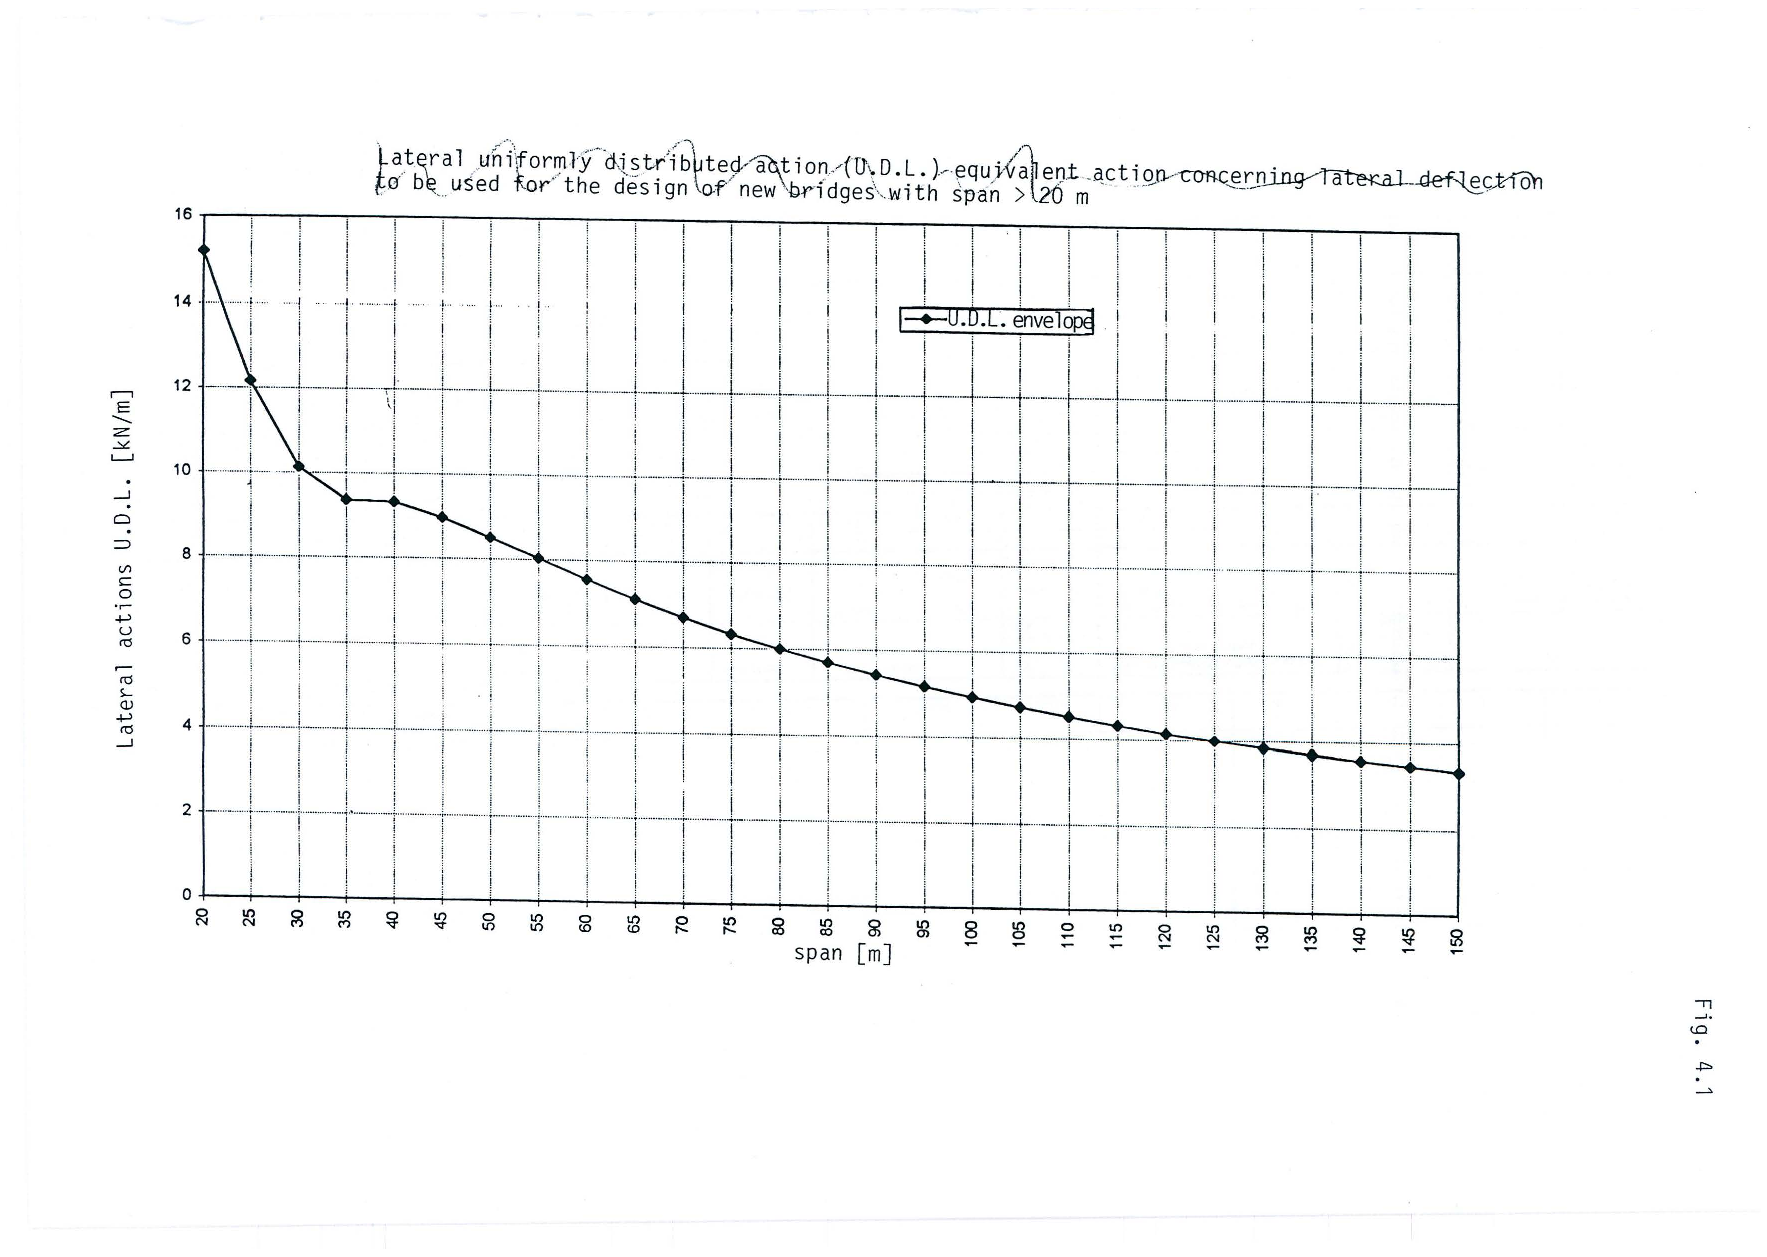
\includegraphics[width=0.8\textwidth]{lateraluniformdistribute}
    \caption{Lateral actions U.D.L. Extracted from \cite[Figure.4.1]{d181} }
    \label{fig:lateralUDL}
\end{figure}

To use this plot in analytical solution, an equivalent concentrated force needed to be converted from uniformly distributed force.

The deflection at mid-span of a simply supported beam loaded by uniformly distributed load $q$ is

$$ \delta = \frac{5}{384} \frac{ql\cdot l^3}{EI} $$

The deflection at mid-span of a simply supported beam loaded by concentrated force $P$ at mid-span is

$$ \delta = \frac{1}{48} \frac{P\cdot l^3}{EI} $$

Thus equivalent concentrated force $P$ can be obtain by 

$$P = \frac{1 \cdot 384}{48 \cdot 5} ql = \frac{5}{8}ql$$

For example, using the alternative load model in Figure.\ref{fig:lateralUDL}, equivalent concentrated force for $120m$ bridge is $\sfrac{5}{8}\cdot 120m \cdot 4kN/m=300kN$. It gives an conservative force output compared to 120kN.

\begin{figure}[h!]
\centering 
\setlength\figureheight{6cm} 
\setlength\figurewidth{6cm} 
% This file was created by matlab2tikz v0.4.7 (commit 29117077607177efe915cc01d961cced006239c8) running on MATLAB 8.3.
% Copyright (c) 2008--2014, Nico Schlmer <nico.schloemer@gmail.com>
% All rights reserved.
% Minimal pgfplots version: 1.3
% 
% The latest updates can be retrieved from
%   http://www.mathworks.com/matlabcentral/fileexchange/22022-matlab2tikz
% where you can also make suggestions and rate matlab2tikz.
% 
\begin{tikzpicture}

\begin{axis}[%
width=\figurewidth,
height=\figureheight,
scale only axis,
xmin=20,
xmax=160,
ymin=300,
ymax=550
]
\addplot [color=blue,solid,forget plot]
  table[row sep=crcr]{%
20	304\\
25	302.5\\
30	300\\
35	329\\
40	374\\
45	405\\
50	425\\
55	440\\
60	456\\
65	461.5\\
70	476\\
75	472.5\\
80	480\\
85	493\\
90	495\\
95	494\\
100	500\\
105	514.5\\
110	495\\
115	494.5\\
120	492\\
125	500\\
130	507\\
135	499.5\\
140	504\\
145	507.5\\
150	510\\
};
\end{axis}
\end{tikzpicture}% 
\caption{Total load verses span calculated from Figure.\ref{fig:lateralUDL}} 
\label{fig:UDL2CL} 
\end{figure}


\section{Alternative analytical model for longer span bridges}
Moving continuous load model can be adopted.

\textbf{Add deduction procedure}

Solution:

\begin{equation}
    v(x,t) = \frac{v_0}{2}(1+\cos \omega t)\sin \frac{\pi x}{l}
\end{equation}

Maximum deflection

\begin{equation}
    v_{max} = v_0
\end{equation}

No dynamics amplification for longer span bridges. Calculate using alternative load model. This is because train speed is far lower than critical speed.

\section{Parametric research}
Since it is concluded in previous chapter that load model is no longer valid when 
span is large, this parametric research will focus on stiffness of the bridge and mass of the bridge. Length of the bridge will be fixed at $54m$.

\subsection{Mass}

The first parameter examined is mass. \textit{Massenvelop.m} is run to iterate calculation. Mass were checked from $1000kg/m$ to $12000kg/m$. Other parameters were $l=54m$, $EJ=2.43e10Nm^2$, $mu=6000kg/m$. The output are presented in Figure.\ref{fig:medefEJ24300000000L54c14min1000max12000} as deflection and Figure.\ref{fig:meaccEJ24300000000L54c14min1000max12000} as acceleration.


\begin{figure}[h!]
\centering 
\setlength\figureheight{6cm} 
\setlength\figurewidth{6cm} 
% This file was created by matlab2tikz v0.4.7 (commit d412d9f5e9b0b532484ca0001381d1809ceeed7a) running on MATLAB 8.3.
% Copyright (c) 2008--2014, Nico Schlmer <nico.schloemer@gmail.com>
% All rights reserved.
% Minimal pgfplots version: 1.3
% 
\begin{tikzpicture}

\begin{axis}[%
width=\figurewidth,
height=\figureheight,
scale only axis,
xmin=0,
xmax=12000,
ymin=0.0166,
ymax=0.018,
title={MassEnvelop def from1000 to12000}
]
\addplot [color=blue,solid,forget plot]
  table[row sep=crcr]{%
1000	0.0178583229931755\\
1100	0.0178890723703288\\
1200	0.0178477938913116\\
1300	0.0178419863715967\\
1400	0.0178503226855626\\
1500	0.0178057070886087\\
1600	0.0177793938397632\\
1700	0.0178110781496719\\
1800	0.0178011687952915\\
1900	0.0177593930329458\\
2000	0.017690417164951\\
2100	0.0177173557748391\\
2200	0.0177417512630887\\
2300	0.0177459404046226\\
2400	0.0177300433934259\\
2500	0.0176911429193898\\
2600	0.0176349425779905\\
2700	0.0175625847284821\\
2800	0.0176015181149876\\
2900	0.0176303894951817\\
3000	0.017646782264091\\
3100	0.0176500358756749\\
3200	0.0176430016709168\\
3300	0.0176246833526256\\
3400	0.0175971952798186\\
3500	0.0175586342557988\\
3600	0.0175106508258149\\
3700	0.0174536475339083\\
3800	0.0173870891942078\\
3900	0.0174165540582186\\
4000	0.0174456419196443\\
4100	0.0174670595177363\\
4200	0.0174822483501605\\
4300	0.017492790060382\\
4400	0.0174967953154319\\
4500	0.0174959220551746\\
4600	0.0174899808936011\\
4700	0.0174780939425474\\
4800	0.0174595492026574\\
4900	0.0174381912491536\\
5000	0.0174106689229747\\
5100	0.017379378710535\\
5200	0.0173417073198063\\
5300	0.0173024210790476\\
5400	0.0172575948917539\\
5500	0.0172080589651557\\
5600	0.0171544242479192\\
5700	0.0170973561577355\\
5800	0.0171193683618762\\
5900	0.0171445730267923\\
6000	0.0171666118764236\\
6100	0.0171862149266261\\
6200	0.0172033848705906\\
6300	0.0172177032604708\\
6400	0.0172290060215173\\
6500	0.0172370950856511\\
6600	0.0172427294995013\\
6700	0.0172471538218133\\
6800	0.0172479137544592\\
6900	0.017246406336062\\
7000	0.0172433412757765\\
7100	0.0172364420911499\\
7200	0.0172293024416101\\
7300	0.0172180757745839\\
7400	0.0172063803970232\\
7500	0.0171915244272861\\
7600	0.017174626684721\\
7700	0.0171565503317906\\
7800	0.0171354631301961\\
7900	0.0171125766200796\\
8000	0.0170887518332896\\
8100	0.0170624855696524\\
8200	0.0170340086886259\\
8300	0.0170035175965923\\
8400	0.0169720950136205\\
8500	0.0169390522470336\\
8600	0.0169041661960147\\
8700	0.0168675382864159\\
8800	0.0168292487699379\\
8900	0.016789358865138\\
9000	0.0167479127194968\\
9100	0.0167049392079755\\
9200	0.0166604535822052\\
9300	0.0166144589832451\\
9400	0.0166086598759013\\
9500	0.0166280646660106\\
9600	0.0166463004737455\\
9700	0.016664054909512\\
9800	0.01668073815691\\
9900	0.0166962801556014\\
10000	0.0167107223074602\\
10100	0.0167240987069877\\
10200	0.0167364367336517\\
10300	0.0167477576019245\\
10400	0.0167580768722198\\
10500	0.0167674049256852\\
10600	0.01677574740558\\
10700	0.0167831056277583\\
10800	0.0167894769625822\\
10900	0.0167948551904097\\
11000	0.0167994698218856\\
11100	0.0168035592379502\\
11200	0.0168066947957504\\
11300	0.0168088558426864\\
11400	0.0168100196855731\\
11500	0.0168101618185837\\
11600	0.0168092561360613\\
11700	0.0168080018529058\\
11800	0.0168061678721097\\
11900	0.0168032557866143\\
12000	0.0167992324434338\\
};
\end{axis}
\end{tikzpicture}% 
\caption{medefEJ24300000000L54c14min1000max12000.tikz} 
\label{fig:medefEJ24300000000L54c14min1000max12000} 
\end{figure}

Incresed mass generally decreases deflection in trend but with a lengthening periodic sinuous wave shape. Further (linear)regression on deflection can be made from peaks.

\begin{figure}[h!]
\centering 
\setlength\figureheight{6cm} 
\setlength\figurewidth{6cm} 
% This file was created by matlab2tikz v0.4.7 (commit d412d9f5e9b0b532484ca0001381d1809ceeed7a) running on MATLAB 8.3.
% Copyright (c) 2008--2014, Nico Schlmer <nico.schloemer@gmail.com>
% All rights reserved.
% Minimal pgfplots version: 1.3
% 
\begin{tikzpicture}

\begin{axis}[%
width=\figurewidth,
height=\figureheight,
scale only axis,
xmin=0,
xmax=12000,
ymin=0,
ymax=7,
title={MassEnvelop acc from1000 to12000}
]
\addplot [color=blue,solid,forget plot]
  table[row sep=crcr]{%
1000	6.08594833830125\\
1100	5.53047003360163\\
1200	5.05456877840365\\
1300	4.67079813703663\\
1400	4.32625615674167\\
1500	4.02672480467682\\
1600	3.78193875211494\\
1700	3.5566315175923\\
1800	3.34898400030217\\
1900	3.1603113220298\\
2000	3.00817887638876\\
2100	2.86662784514866\\
2200	2.73398551857465\\
2300	2.61011857745419\\
2400	2.49347778171561\\
2500	2.38370381345109\\
2600	2.29415871452593\\
2700	2.21195247203\\
2800	2.13378576910117\\
2900	2.05963275694185\\
3000	1.98910884831677\\
3100	1.92162982933649\\
3200	1.85746688058188\\
3300	1.79583909905011\\
3400	1.73700745855225\\
3500	1.68068358447949\\
3600	1.63676318631786\\
3700	1.59428922352765\\
3800	1.5536859445795\\
3900	1.51433010873051\\
4000	1.47648133722729\\
4100	1.44005551086797\\
4200	1.40483065356283\\
4300	1.37076129090895\\
4400	1.33777083636434\\
4500	1.30598345208441\\
4600	1.27521557799511\\
4700	1.24526443081149\\
4800	1.21638888350873\\
4900	1.18824922352\\
5000	1.16110192003383\\
5100	1.13462988818833\\
5200	1.11017171784746\\
5300	1.09048715269058\\
5400	1.07131105318258\\
5500	1.05273609538422\\
5600	1.03461679372124\\
5700	1.01694133200062\\
5800	0.999694376793413\\
5900	0.982856140128679\\
6000	0.966456968399831\\
6100	0.950485133832355\\
6200	0.93486870666344\\
6300	0.919577018933324\\
6400	0.904605762535865\\
6500	0.890083007545826\\
6600	0.875805361289476\\
6700	0.861859787935206\\
6800	0.848238048587338\\
6900	0.834873713196433\\
7000	0.821830812785818\\
7100	0.809049470870249\\
7200	0.796502391784864\\
7300	0.784286252011837\\
7400	0.772265478540667\\
7500	0.760469285947375\\
7600	0.748981227553528\\
7700	0.737693813210901\\
7800	0.726611533337861\\
7900	0.71573661261543\\
8000	0.705069351789242\\
8100	0.694626972136538\\
8200	0.684391886435546\\
8300	0.674344468670962\\
8400	0.666118507921187\\
8500	0.658820557974586\\
8600	0.651623756745264\\
8700	0.644546892971819\\
8800	0.637627736123581\\
8900	0.630807706584579\\
9000	0.624088317428015\\
9100	0.617470387087868\\
9200	0.610954127579355\\
9300	0.604539223197536\\
9400	0.598231128933985\\
9500	0.592033631654554\\
9600	0.585928090559521\\
9700	0.579913119903328\\
9800	0.573987062210478\\
9900	0.568148029414578\\
10000	0.562393939504866\\
10100	0.556722549149172\\
10200	0.551131482713258\\
10300	0.545638078051018\\
10400	0.540223460128508\\
10500	0.534884547931594\\
10600	0.529618437044497\\
10700	0.524422207565185\\
10800	0.519292937226712\\
10900	0.514227712921362\\
11000	0.509247288507103\\
11100	0.504345676019317\\
11200	0.499501143319295\\
11300	0.494710756151831\\
11400	0.489979625996909\\
11500	0.485342235316628\\
11600	0.480751556569492\\
11700	0.476204792487503\\
11800	0.471737713000062\\
11900	0.467330526932989\\
12000	0.462959865836589\\
};
\end{axis}
\end{tikzpicture}% 
\caption{meaccEJ24300000000L54c14min1000max12000.tikz} 
\label{fig:meaccEJ24300000000L54c14min1000max12000} 
\end{figure}

The acceleration simply decreases as mass increases.

\subsection{Stiffness}

The next parameter examined is stiffness. \textit{Speedenvelop.m} is run to iterate calculation. Stiffness were checked from $2e10 Nm^2$ to $3e11 Nm^2$ Other parameters are $l=54m$, $mu=4000kg/m$, $c=14m/s$. The output is presented in Figure.\ref{fig:stedefmin20000000000max300000000000L54c14mu4000} as deflection and Figure.\ref{fig:steaccmin20000000000max300000000000L54c14mu4000} as acceleration. 



\begin{figure}[h!]
\centering 
\setlength\figureheight{6cm} 
\setlength\figurewidth{6cm} 
% This file was created by matlab2tikz v0.4.7 (commit 29117077607177efe915cc01d961cced006239c8) running on MATLAB 8.3.
% Copyright (c) 2008--2014, Nico Schlmer <nico.schloemer@gmail.com>
% All rights reserved.
% Minimal pgfplots version: 1.3
% 
\begin{tikzpicture}

\begin{axis}[%
width=\figurewidth,
height=\figureheight,
scale only axis,
xmin=0,
xmax=300000000000,
ymin=0,
ymax=0.025,
title={StiffEnvelop def from20000000000 to300000000000}
]
\addplot [color=blue,solid,forget plot]
  table[row sep=crcr]{%
20000000000	0.0211975023937896\\
21000000000	0.0202352112023207\\
22000000000	0.01932783813784\\
23000000000	0.0184749121479239\\
24000000000	0.017675537909681\\
25000000000	0.0169253433921581\\
26000000000	0.0162887243975358\\
27000000000	0.0157595857432334\\
28000000000	0.0152465973021956\\
29000000000	0.0147555923738135\\
30000000000	0.0142866703650115\\
31000000000	0.0138350279514467\\
32000000000	0.0134016390839295\\
33000000000	0.0129875805416541\\
34000000000	0.012593190882245\\
35000000000	0.012213705287707\\
36000000000	0.0118547446917254\\
37000000000	0.011571640759037\\
38000000000	0.0112934612366699\\
39000000000	0.0110247158546545\\
40000000000	0.0107647721160318\\
41000000000	0.0105117873084173\\
42000000000	0.0102672406599101\\
43000000000	0.0100295319854085\\
44000000000	0.00979780036723733\\
45000000000	0.00957733476372697\\
46000000000	0.00936158487933822\\
47000000000	0.00915288052120197\\
48000000000	0.00895152382982422\\
49000000000	0.00877911034212504\\
50000000000	0.00861755392140512\\
51000000000	0.00846047178190724\\
52000000000	0.00830738448409933\\
53000000000	0.00815870028033678\\
54000000000	0.00801052595788117\\
55000000000	0.00786919353707517\\
56000000000	0.00772946316972668\\
57000000000	0.00759300501655167\\
58000000000	0.00746036593688397\\
59000000000	0.00733112045324021\\
60000000000	0.00720400506251978\\
61000000000	0.00708063492856119\\
62000000000	0.00696085638792835\\
63000000000	0.00685355050653496\\
64000000000	0.00675318179213945\\
65000000000	0.00665808920967364\\
66000000000	0.00656160598872018\\
67000000000	0.00646920437067868\\
68000000000	0.00637599944652451\\
69000000000	0.00628584747955797\\
70000000000	0.00619822985668251\\
71000000000	0.00611169397982591\\
72000000000	0.00602649217324711\\
73000000000	0.00594247486611201\\
74000000000	0.00585956388301908\\
75000000000	0.00578102944611349\\
76000000000	0.00570260645185775\\
77000000000	0.00562369823446464\\
78000000000	0.00554999516747907\\
79000000000	0.00547954067581213\\
80000000000	0.0054172766159893\\
81000000000	0.00535433816739347\\
82000000000	0.00529118772986884\\
83000000000	0.00523163669143009\\
84000000000	0.00517017944299437\\
85000000000	0.00511197015586434\\
86000000000	0.00505394722886256\\
87000000000	0.00499514251339443\\
88000000000	0.00493898394214433\\
89000000000	0.00488424447716478\\
90000000000	0.00482977871228434\\
91000000000	0.00477592778473705\\
92000000000	0.0047228750197933\\
93000000000	0.00467065947511198\\
94000000000	0.00461918854864043\\
95000000000	0.00456824970433047\\
96000000000	0.00451752140663701\\
97000000000	0.00447264082792648\\
98000000000	0.00442974331638533\\
99000000000	0.00438703733456374\\
100000000000	0.00434453714871276\\
101000000000	0.00430433827019271\\
102000000000	0.00426443955256094\\
103000000000	0.00422441219917602\\
104000000000	0.00418374808334528\\
105000000000	0.00414405535544843\\
106000000000	0.00410663681194211\\
107000000000	0.00406734164254742\\
108000000000	0.00403003448772119\\
109000000000	0.00399296151969919\\
110000000000	0.00395559778161519\\
111000000000	0.00391982075868934\\
112000000000	0.00388378172300036\\
113000000000	0.0038478965922779\\
114000000000	0.00381400823467746\\
115000000000	0.00377807597589494\\
116000000000	0.00374516047703937\\
117000000000	0.00371380414073606\\
118000000000	0.00368542745884508\\
119000000000	0.0036538552831394\\
120000000000	0.00362667954526633\\
121000000000	0.00359748136491447\\
122000000000	0.00356764786135987\\
123000000000	0.00354100221711498\\
124000000000	0.00351302607020401\\
125000000000	0.00348414096907457\\
126000000000	0.003456785940834\\
127000000000	0.00343077284331492\\
128000000000	0.00340433713404623\\
129000000000	0.00337771852841288\\
130000000000	0.00335111555863198\\
131000000000	0.00332468787845705\\
132000000000	0.00329855849540191\\
133000000000	0.00327281591667227\\
134000000000	0.00324751619993797\\
135000000000	0.00322268490437177\\
136000000000	0.0031983189410869\\
137000000000	0.00317438832528405\\
138000000000	0.00315083783512515\\
139000000000	0.00312918139121786\\
140000000000	0.00310824549432802\\
141000000000	0.003087300997505\\
142000000000	0.00306637407236676\\
143000000000	0.00304546515629223\\
144000000000	0.00302455039244248\\
145000000000	0.00300446935959938\\
146000000000	0.00298492962126159\\
147000000000	0.00296554415094883\\
148000000000	0.00294619877435489\\
149000000000	0.00292676135586058\\
150000000000	0.00290708292133887\\
151000000000	0.00288699876507276\\
152000000000	0.00286688286285168\\
153000000000	0.0028494062376335\\
154000000000	0.00283126755105162\\
155000000000	0.00281224252505524\\
156000000000	0.00279209613408547\\
157000000000	0.0027755707011171\\
158000000000	0.00275796856902784\\
159000000000	0.00273877550069635\\
160000000000	0.00272160356712225\\
161000000000	0.0027047992643237\\
162000000000	0.00268846904233831\\
163000000000	0.00267127628982741\\
164000000000	0.00265663945493392\\
165000000000	0.00264193657537714\\
166000000000	0.00262568602257958\\
167000000000	0.00261004762256232\\
168000000000	0.00259617788878515\\
169000000000	0.00258022564628786\\
170000000000	0.00256535445760045\\
171000000000	0.00255145259348965\\
172000000000	0.0025348494688459\\
173000000000	0.00252211771175436\\
174000000000	0.00250704467559132\\
175000000000	0.00249282762651141\\
176000000000	0.00247901321748457\\
177000000000	0.00246400089495544\\
178000000000	0.00245109952803561\\
179000000000	0.00243588405770447\\
180000000000	0.00242348350172451\\
181000000000	0.0024085666880646\\
182000000000	0.0023961948390819\\
183000000000	0.00238199533928957\\
184000000000	0.00236912643052633\\
185000000000	0.00235598640681731\\
186000000000	0.00234204682869739\\
187000000000	0.00233074114644216\\
188000000000	0.00231751191009128\\
189000000000	0.00230709948417153\\
190000000000	0.00229433859694933\\
191000000000	0.00228362945185648\\
192000000000	0.00227170215292621\\
193000000000	0.00226017043949403\\
194000000000	0.00224937508539725\\
195000000000	0.00223645230328921\\
196000000000	0.00222702523201832\\
197000000000	0.0022146638429713\\
198000000000	0.00220422500697117\\
199000000000	0.00219367623371104\\
200000000000	0.00218067534431702\\
201000000000	0.00217182090613048\\
202000000000	0.00216094867190641\\
203000000000	0.00214845822098414\\
204000000000	0.00213973861759207\\
205000000000	0.00212915651790653\\
206000000000	0.00211688144454458\\
207000000000	0.00210800470365984\\
208000000000	0.00209816107539982\\
209000000000	0.00208691459134001\\
210000000000	0.00207622852917882\\
211000000000	0.00206742403110474\\
212000000000	0.00205745541680753\\
213000000000	0.0020464465815816\\
214000000000	0.00203720246244118\\
215000000000	0.00202885819701527\\
216000000000	0.00201893592710437\\
217000000000	0.00200932996342407\\
218000000000	0.00200178170973001\\
219000000000	0.00199291047563808\\
220000000000	0.00198284420465172\\
221000000000	0.00197427855077842\\
222000000000	0.00196664674976842\\
223000000000	0.0019580141267412\\
224000000000	0.00194848748581229\\
225000000000	0.00193905380842901\\
226000000000	0.00193189296241654\\
227000000000	0.0019239793496787\\
228000000000	0.00191540089812732\\
229000000000	0.00190624111710506\\
230000000000	0.00189664189299943\\
231000000000	0.00188967935168239\\
232000000000	0.00188221848109409\\
233000000000	0.0018743265533631\\
234000000000	0.0018660669393803\\
235000000000	0.00185749918200361\\
236000000000	0.00184867907579742\\
237000000000	0.00184008933337732\\
238000000000	0.00183308995460331\\
239000000000	0.0018258528420375\\
240000000000	0.00181842085621405\\
241000000000	0.00181083363333262\\
242000000000	0.00180312766937039\\
243000000000	0.00179533640553938\\
244000000000	0.00178749031448496\\
245000000000	0.00177962441419596\\
246000000000	0.00177354164330591\\
247000000000	0.00176717797284885\\
248000000000	0.00176057832710289\\
249000000000	0.00175378457332746\\
250000000000	0.00174683559127907\\
251000000000	0.0017397673450976\\
252000000000	0.00173261295691221\\
253000000000	0.00172540278158209\\
254000000000	0.0017181644820496\\
255000000000	0.00171092310484237\\
256000000000	0.00170475458149119\\
257000000000	0.00169856910362668\\
258000000000	0.00169232664078591\\
259000000000	0.00168604359405507\\
260000000000	0.00167973411730581\\
261000000000	0.00167341018236327\\
262000000000	0.00166708164318647\\
263000000000	0.00166075629892797\\
264000000000	0.00165443995577315\\
265000000000	0.00164813648748976\\
266000000000	0.0016418478946467\\
267000000000	0.00163557436248769\\
268000000000	0.00162931431746953\\
269000000000	0.00162306448249736\\
270000000000	0.00161681993091001\\
271000000000	0.00161057413928762\\
272000000000	0.00160431903917113\\
273000000000	0.0015980450677995\\
274000000000	0.00159174121798472\\
275000000000	0.00158599457813231\\
276000000000	0.0015804338836043\\
277000000000	0.00157485632363192\\
278000000000	0.00156926030745324\\
279000000000	0.00156364266689394\\
280000000000	0.00155799870355807\\
281000000000	0.00155238193301926\\
282000000000	0.00154727403433425\\
283000000000	0.00154221252448781\\
284000000000	0.00153718618081228\\
285000000000	0.00153218246839402\\
286000000000	0.00152718757999456\\
287000000000	0.001522186475438\\
288000000000	0.00151716292062633\\
289000000000	0.00151209952635278\\
290000000000	0.00150697778708988\\
291000000000	0.00150177811993545\\
292000000000	0.00149647990390472\\
293000000000	0.00149106151976135\\
294000000000	0.00148550039058381\\
295000000000	0.00147977302326633\\
296000000000	0.00147407835006431\\
297000000000	0.00146990153252398\\
298000000000	0.00146556624132945\\
299000000000	0.0014610446133361\\
300000000000	0.00145630801477946\\
};
\end{axis}
\end{tikzpicture}% 
\caption{stedefmin20000000000max300000000000L54c14mu4000.tikz} 
\label{fig:stedefmin20000000000max300000000000L54c14mu4000} 
\end{figure}


\begin{figure}[h!]
\centering 
\setlength\figureheight{6cm} 
\setlength\figurewidth{6cm} 
% This file was created by matlab2tikz v0.4.7 (commit d412d9f5e9b0b532484ca0001381d1809ceeed7a) running on MATLAB 8.3.
% Copyright (c) 2008--2014, Nico Schlmer <nico.schloemer@gmail.com>
% All rights reserved.
% Minimal pgfplots version: 1.3
% 
\begin{tikzpicture}

\begin{axis}[%
width=\figurewidth,
height=\figureheight,
scale only axis,
xmin=0,
xmax=300000000000,
ymin=1.45,
ymax=1.55,
title={StiffEnvelop acc from20000000000 to300000000000}
]
\addplot [color=blue,solid,forget plot]
  table[row sep=crcr]{%
20000000000	1.45734013072347\\
21000000000	1.46561454900335\\
22000000000	1.4712594854351\\
23000000000	1.47464034316331\\
24000000000	1.47640674991883\\
25000000000	1.47634178613263\\
26000000000	1.47516383090184\\
27000000000	1.47308686768607\\
28000000000	1.47253961862366\\
29000000000	1.47917798778388\\
30000000000	1.48436540000659\\
31000000000	1.48827360243856\\
32000000000	1.49091906098922\\
33000000000	1.49269714011968\\
34000000000	1.49358617523083\\
35000000000	1.49370536032551\\
36000000000	1.49306791862025\\
37000000000	1.49168857082641\\
38000000000	1.48995050647699\\
39000000000	1.49034142798257\\
40000000000	1.49410041315658\\
41000000000	1.49768530182124\\
42000000000	1.50031262711091\\
43000000000	1.50224604235569\\
44000000000	1.50342419637148\\
45000000000	1.5045590176152\\
46000000000	1.50501412772669\\
47000000000	1.5050064363811\\
48000000000	1.50458025831697\\
49000000000	1.50345819905747\\
50000000000	1.50278016736726\\
51000000000	1.50127476550373\\
52000000000	1.50221176994358\\
53000000000	1.50500789786271\\
54000000000	1.50704280013598\\
55000000000	1.50898601880754\\
56000000000	1.51032001749145\\
57000000000	1.51133950201605\\
58000000000	1.51213854637151\\
59000000000	1.51262117420061\\
60000000000	1.51251171071252\\
61000000000	1.51267954629584\\
62000000000	1.51214476621485\\
63000000000	1.51190960768996\\
64000000000	1.51109074122402\\
65000000000	1.50999530315438\\
66000000000	1.50896179583705\\
67000000000	1.51093501331824\\
68000000000	1.51217799215585\\
69000000000	1.51391521113948\\
70000000000	1.51524954670985\\
71000000000	1.5162537916239\\
72000000000	1.51697559762201\\
73000000000	1.51736476174323\\
74000000000	1.51758823575617\\
75000000000	1.51820798437198\\
76000000000	1.51819973989772\\
77000000000	1.51787324934807\\
78000000000	1.51789553101621\\
79000000000	1.51731922955448\\
80000000000	1.51673580239897\\
81000000000	1.5163706335211\\
82000000000	1.51546368124005\\
83000000000	1.5158029435943\\
84000000000	1.51649495035764\\
85000000000	1.51819208018441\\
86000000000	1.51914592526996\\
87000000000	1.51950680915957\\
88000000000	1.52042315007333\\
89000000000	1.52122232922279\\
90000000000	1.52173467258494\\
91000000000	1.52205947617053\\
92000000000	1.52225050200008\\
93000000000	1.52231752865413\\
94000000000	1.52222788367035\\
95000000000	1.52190795625925\\
96000000000	1.52124470225895\\
97000000000	1.52133601255633\\
98000000000	1.52121860493315\\
99000000000	1.52049681131391\\
100000000000	1.51968184854689\\
101000000000	1.51951511396415\\
102000000000	1.52050828294162\\
103000000000	1.52159512133696\\
104000000000	1.52213546838458\\
105000000000	1.5224739324904\\
106000000000	1.52364589336719\\
107000000000	1.52379049958592\\
108000000000	1.52433271608226\\
109000000000	1.52472616219795\\
110000000000	1.52478634199077\\
111000000000	1.52507745495476\\
112000000000	1.52517632423383\\
113000000000	1.52480780217682\\
114000000000	1.52527520801483\\
115000000000	1.52470006154758\\
116000000000	1.52448168263523\\
117000000000	1.52465333252103\\
118000000000	1.52418885411005\\
119000000000	1.52324781690574\\
120000000000	1.52295683401026\\
121000000000	1.52285074686318\\
122000000000	1.52305147448529\\
123000000000	1.52430571512629\\
124000000000	1.52483130785261\\
125000000000	1.52479386989337\\
126000000000	1.52545467249412\\
127000000000	1.52629508459255\\
128000000000	1.52678092640726\\
129000000000	1.52701187348561\\
130000000000	1.52707237211512\\
131000000000	1.52703196013823\\
132000000000	1.52694560161109\\
133000000000	1.52685402758201\\
134000000000	1.52678407714971\\
135000000000	1.52674903470079\\
136000000000	1.5267489608253\\
137000000000	1.52677101587813\\
138000000000	1.52678977649978\\
139000000000	1.52676754664047\\
140000000000	1.52665466575462\\
141000000000	1.52638981785403\\
142000000000	1.52590034603378\\
143000000000	1.52510257791843\\
144000000000	1.52512990481664\\
145000000000	1.52545371448326\\
146000000000	1.52632398094211\\
147000000000	1.52712851434398\\
148000000000	1.527806444945\\
149000000000	1.52828594532712\\
150000000000	1.52848449686605\\
151000000000	1.52830917339089\\
152000000000	1.52795307703176\\
153000000000	1.52890596680527\\
154000000000	1.529349583793\\
155000000000	1.52915192238829\\
156000000000	1.5282315885808\\
157000000000	1.5292655887501\\
158000000000	1.52941319324496\\
159000000000	1.52850690833346\\
160000000000	1.52895028907703\\
161000000000	1.52910580791489\\
162000000000	1.52786196764924\\
163000000000	1.52864197779296\\
164000000000	1.5282544313577\\
165000000000	1.52758801942517\\
166000000000	1.52796397697837\\
167000000000	1.52664500897598\\
168000000000	1.52801007951756\\
169000000000	1.5280086703519\\
170000000000	1.52821914745711\\
171000000000	1.52921439025087\\
172000000000	1.52844019281204\\
173000000000	1.52971563152382\\
174000000000	1.52963089789829\\
175000000000	1.52985858362243\\
176000000000	1.53031013172611\\
177000000000	1.52989054310104\\
178000000000	1.53067484625713\\
179000000000	1.52996325376503\\
180000000000	1.53082838870446\\
181000000000	1.53013627963491\\
182000000000	1.53078375277264\\
183000000000	1.5303803069534\\
184000000000	1.53046682012303\\
185000000000	1.53058034022684\\
186000000000	1.52971958500226\\
187000000000	1.53053881768339\\
188000000000	1.52930140818064\\
189000000000	1.529978724314\\
190000000000	1.5297775081126\\
191000000000	1.52854682649245\\
192000000000	1.52947842366165\\
193000000000	1.52889684225918\\
194000000000	1.52950492770267\\
195000000000	1.52892345263538\\
196000000000	1.53034668982061\\
197000000000	1.5296997811816\\
198000000000	1.53053232637812\\
199000000000	1.53101044165937\\
200000000000	1.52971425395408\\
201000000000	1.53136977963361\\
202000000000	1.53143421821037\\
203000000000	1.53029297326263\\
204000000000	1.53175594792709\\
205000000000	1.53183325898967\\
206000000000	1.53062673441562\\
207000000000	1.53169078497265\\
208000000000	1.53210715343718\\
209000000000	1.53143712902145\\
210000000000	1.53086908145943\\
211000000000	1.53185471993367\\
212000000000	1.53192168737936\\
213000000000	1.5311494653261\\
214000000000	1.5303887864271\\
215000000000	1.53130283537239\\
216000000000	1.53150788258114\\
217000000000	1.53107162542902\\
218000000000	1.53005927566858\\
219000000000	1.52991583604698\\
220000000000	1.53034830809788\\
221000000000	1.53049161437033\\
222000000000	1.5309917282491\\
223000000000	1.53121786291905\\
224000000000	1.53069454795767\\
225000000000	1.5304092503752\\
226000000000	1.53163133150458\\
227000000000	1.53221502282741\\
228000000000	1.53222195071971\\
229000000000	1.53171144564974\\
230000000000	1.53083954266215\\
231000000000	1.53197517980801\\
232000000000	1.53266411484586\\
233000000000	1.53295541437947\\
234000000000	1.53289590534238\\
235000000000	1.53253016695707\\
236000000000	1.53190052948261\\
237000000000	1.53122920795054\\
238000000000	1.5319827944811\\
239000000000	1.5324913134901\\
240000000000	1.53278778415783\\
241000000000	1.53290311553704\\
242000000000	1.53286612079652\\
243000000000	1.53270353431166\\
244000000000	1.53244003112873\\
245000000000	1.53209824837172\\
246000000000	1.53169880820102\\
247000000000	1.53126034197208\\
248000000000	1.53112409941318\\
249000000000	1.5314515296061\\
250000000000	1.53160226665764\\
251000000000	1.53160573989086\\
252000000000	1.53148938542794\\
253000000000	1.53127866232774\\
254000000000	1.53099707075278\\
255000000000	1.53080986962944\\
256000000000	1.53142177650973\\
257000000000	1.53192565321651\\
258000000000	1.5323371124945\\
259000000000	1.53266993738345\\
260000000000	1.53293610023239\\
261000000000	1.53314578232529\\
262000000000	1.53330739395146\\
263000000000	1.53342759478085\\
264000000000	1.53351131443122\\
265000000000	1.53356177313937\\
266000000000	1.53358050247273\\
267000000000	1.53356736604099\\
268000000000	1.53352058018982\\
269000000000	1.53343673467958\\
270000000000	1.53331081337286\\
271000000000	1.53313621497356\\
272000000000	1.53290477387922\\
273000000000	1.53260678122555\\
274000000000	1.53223100621951\\
275000000000	1.53176471787248\\
276000000000	1.53119370726125\\
277000000000	1.53149395452861\\
278000000000	1.53185357137806\\
279000000000	1.53215707678138\\
280000000000	1.53238457315222\\
281000000000	1.53251476219703\\
282000000000	1.53252496696902\\
283000000000	1.53239115528158\\
284000000000	1.53208796471261\\
285000000000	1.53224000238615\\
286000000000	1.53272643996329\\
287000000000	1.53316867293913\\
288000000000	1.53354979509217\\
289000000000	1.53385150056554\\
290000000000	1.53405410273862\\
291000000000	1.53413655413807\\
292000000000	1.53407646758892\\
293000000000	1.53385013881602\\
294000000000	1.53343257071536\\
295000000000	1.53279749952304\\
296000000000	1.53220891683983\\
297000000000	1.53312880493112\\
298000000000	1.53384642396221\\
299000000000	1.53433042679518\\
300000000000	1.5345482610467\\
};
\end{axis}
\end{tikzpicture}% 
\caption{steaccmin20000000000max300000000000L54c14mu4000} 
\label{fig:steaccmin20000000000max300000000000L54c14mu4000} 
\end{figure}

In addition, dynamic coefficient is plotted in Figure.\ref{fig:steacomin20000000000max300000000000L54c14mu4000}. Dynamic coefficient becomes relevant in stiffness case.This is because stiffness is relevant to static deflection. Static deflection decreases as stiffness increases. 

The dynamic coefficient is an indication for the amplification level of resonance effect. Usually symboled as $\delta$, dynamic coefficient is simply the ratio of the maximum dynamic deflection to the static deflection at mid-span of a beam:

$$\delta = \frac{MAX v(\sfrac{l}{2},t )}{v_0}$$

\begin{figure}[h!]
\centering 
\setlength\figureheight{6cm} 
\setlength\figurewidth{6cm} 
% This file was created by matlab2tikz v0.4.7 (commit 29117077607177efe915cc01d961cced006239c8) running on MATLAB 8.3.
% Copyright (c) 2008--2014, Nico Schlmer <nico.schloemer@gmail.com>
% All rights reserved.
% Minimal pgfplots version: 1.3
% 
\begin{tikzpicture}

\begin{axis}[%
width=\figurewidth,
height=\figureheight,
scale only axis,
xmin=0,
xmax=300000000000,
ymin=1.31,
ymax=1.37,
title={StiffEnvelop dc from20000000000 to300000000000}
]
\addplot [color=blue,solid,forget plot]
  table[row sep=crcr]{%
20000000000	1.31481735587447\\
21000000000	1.31788579211158\\
22000000000	1.31873247231574\\
23000000000	1.31783475677695\\
24000000000	1.31563258272585\\
25000000000	1.31228521836756\\
26000000000	1.31344279569341\\
27000000000	1.31965163804388\\
28000000000	1.32398084123158\\
29000000000	1.32710530957295\\
30000000000	1.32923882761853\\
31000000000	1.33012505549215\\
32000000000	1.33002142138244\\
33000000000	1.32920795964996\\
34000000000	1.32790022010016\\
35000000000	1.32576399514436\\
36000000000	1.32356552225107\\
37000000000	1.32784507217275\\
38000000000	1.33094896160112\\
39000000000	1.3334684712377\\
40000000000	1.33541291301742\\
41000000000	1.33662986714678\\
42000000000	1.33737675921406\\
43000000000	1.33751870072155\\
44000000000	1.33700183221701\\
45000000000	1.33661989544718\\
46000000000	1.33554323113745\\
47000000000	1.33415531526307\\
48000000000	1.33256667782805\\
49000000000	1.33412747217545\\
50000000000	1.33630241555807\\
51000000000	1.33818296487336\\
52000000000	1.33973342975171\\
53000000000	1.34105808346246\\
54000000000	1.3415458850433\\
55000000000	1.3422816579731\\
56000000000	1.34241902594876\\
57000000000	1.34226814044364\\
58000000000	1.34195781441706\\
59000000000	1.34144572700292\\
60000000000	1.34052833848722\\
61000000000	1.33953102782066\\
62000000000	1.33845909408487\\
63000000000	1.33908118098303\\
64000000000	1.34041461492661\\
65000000000	1.34218909536785\\
66000000000	1.34308909659057\\
67000000000	1.34423875942072\\
68000000000	1.34464587213325\\
69000000000	1.34512817458097\\
70000000000	1.34560148358733\\
71000000000	1.34576952277743\\
72000000000	1.34569870006451\\
73000000000	1.34536756508723\\
74000000000	1.34476919724145\\
75000000000	1.34467454750677\\
76000000000	1.34411903958647\\
77000000000	1.34296122421517\\
78000000000	1.34257311824149\\
79000000000	1.34252377677808\\
80000000000	1.34406953875141\\
81000000000	1.34505968272843\\
82000000000	1.34560552737974\\
83000000000	1.34668619745879\\
84000000000	1.3469008971467\\
85000000000	1.34759060642214\\
86000000000	1.34796896622853\\
87000000000	1.34777648710949\\
88000000000	1.34794144245242\\
89000000000	1.34814976494699\\
90000000000	1.34809495056939\\
91000000000	1.34787582255204\\
92000000000	1.34755040850284\\
93000000000	1.34713739979151\\
94000000000	1.34661758996973\\
95000000000	1.34593528788391\\
96000000000	1.3449997134125\\
97000000000	1.34550866124851\\
98000000000	1.34634194645394\\
99000000000	1.34696795735313\\
100000000000	1.34739290041135\\
101000000000	1.34827508063185\\
102000000000	1.34900287148828\\
103000000000	1.34944209131353\\
104000000000	1.34942765190313\\
105000000000	1.34947730964208\\
106000000000	1.35002838767651\\
107000000000	1.3497246219067\\
108000000000	1.34984299707955\\
109000000000	1.34980913335939\\
110000000000	1.3494461214013\\
111000000000	1.34939757981026\\
112000000000	1.34903611366121\\
113000000000	1.3485050445896\\
114000000000	1.34845735769636\\
115000000000	1.34747050348974\\
116000000000	1.34734607147383\\
117000000000	1.3475832289862\\
118000000000	1.34871632470912\\
119000000000	1.3484940774919\\
120000000000	1.34971218450004\\
121000000000	1.35000278010736\\
122000000000	1.34987188432851\\
123000000000	1.35077200027789\\
124000000000	1.35099517340313\\
125000000000	1.35069244578629\\
126000000000	1.35080845924862\\
127000000000	1.35128334584221\\
128000000000	1.35142911565757\\
129000000000	1.351337740614\\
130000000000	1.351087562353\\
131000000000	1.35074358996921\\
132000000000	1.35035781095554\\
133000000000	1.34996950809197\\
134000000000	1.34960557671958\\
135000000000	1.34928083841909\\
136000000000	1.34899834856238\\
137000000000	1.34874969653511\\
138000000000	1.34851529864374\\
139000000000	1.34895132401087\\
140000000000	1.34956587452534\\
141000000000	1.35004680529711\\
142000000000	1.35040556207418\\
143000000000	1.35064250231888\\
144000000000	1.35074713925877\\
145000000000	1.35109697345994\\
146000000000	1.35156734760946\\
147000000000	1.35198685318234\\
148000000000	1.35230451951712\\
149000000000	1.35245965963195\\
150000000000	1.35238211403474\\
151000000000	1.35199250798648\\
152000000000	1.35146336074718\\
153000000000	1.35206179471902\\
154000000000	1.35223562073044\\
155000000000	1.35187086640664\\
156000000000	1.35084557735637\\
157000000000	1.35145841385227\\
158000000000	1.35144115121573\\
159000000000	1.35053019395126\\
160000000000	1.35050310716251\\
161000000000	1.35055307243868\\
162000000000	1.35073699271898\\
163000000000	1.35038359510812\\
164000000000	1.35122355029455\\
165000000000	1.35193892104033\\
166000000000	1.3517663148363\\
167000000000	1.35180996081205\\
168000000000	1.35267812891691\\
169000000000	1.35236876589327\\
170000000000	1.35253041930994\\
171000000000	1.35311389389103\\
172000000000	1.35217020017605\\
173000000000	1.35320064064815\\
174000000000	1.35288867408064\\
175000000000	1.35294778917597\\
176000000000	1.35313849624868\\
177000000000	1.3525859353771\\
178000000000	1.35310559003839\\
179000000000	1.35226056633491\\
180000000000	1.35289257172522\\
181000000000	1.35203517329688\\
182000000000	1.35252174458927\\
183000000000	1.35189429929455\\
184000000000	1.3519380783404\\
185000000000	1.3517464832959\\
186000000000	1.35101216083654\\
187000000000	1.35171890957864\\
188000000000	1.35123399715381\\
189000000000	1.35231811553617\\
190000000000	1.35195380281462\\
191000000000	1.35272570358628\\
192000000000	1.35270581790951\\
193000000000	1.35284873263348\\
194000000000	1.35336315892001\\
195000000000	1.35252403471426\\
196000000000	1.35372967304309\\
197000000000	1.35308407000541\\
198000000000	1.35354236983346\\
199000000000	1.35386807087573\\
200000000000	1.35260736711867\\
201000000000	1.35385080139363\\
202000000000	1.35377522023866\\
203000000000	1.35261341473936\\
204000000000	1.35375985697001\\
205000000000	1.35366808239416\\
206000000000	1.35242906653202\\
207000000000	1.35329557148664\\
208000000000	1.35348329626359\\
209000000000	1.35270065797142\\
210000000000	1.35221325462009\\
211000000000	1.35289083575306\\
212000000000	1.35274841495194\\
213000000000	1.35185700490342\\
214000000000	1.3520685327253\\
215000000000	1.35282273568103\\
216000000000	1.35246808981784\\
217000000000	1.35226477093991\\
218000000000	1.35339307501711\\
219000000000	1.35357599709981\\
220000000000	1.35288852357366\\
221000000000	1.35316713238982\\
222000000000	1.3540355683848\\
223000000000	1.35416449712004\\
224000000000	1.35361880396669\\
225000000000	1.35307889022784\\
226000000000	1.35407350117152\\
227000000000	1.35449374296028\\
228000000000	1.35439478632192\\
229000000000	1.35382975465708\\
230000000000	1.35289444828821\\
231000000000	1.35378855143235\\
232000000000	1.35428091357107\\
233000000000	1.35441551003864\\
234000000000	1.35423431951697\\
235000000000	1.35377731689296\\
236000000000	1.35308247226089\\
237000000000	1.35250224112369\\
238000000000	1.35304261156648\\
239000000000	1.3533633533123\\
240000000000	1.35349415659545\\
241000000000	1.35346283340316\\
242000000000	1.35329533060495\\
243000000000	1.35301574566095\\
244000000000	1.35264634448146\\
245000000000	1.35221322469349\\
246000000000	1.3530917216179\\
247000000000	1.35371731049896\\
248000000000	1.35412193065566\\
249000000000	1.35433571797049\\
250000000000	1.35438701138316\\
251000000000	1.35430236252321\\
252000000000	1.35410654802427\\
253000000000	1.35382258409841\\
254000000000	1.35347174298366\\
255000000000	1.35307357091153\\
256000000000	1.35348227027068\\
257000000000	1.35383919459183\\
258000000000	1.35411215582553\\
259000000000	1.35431379794627\\
260000000000	1.35445515634699\\
261000000000	1.35454567574261\\
262000000000	1.35459322848345\\
263000000000	1.35460413314907\\
264000000000	1.35458317331614\\
265000000000	1.35453361641711\\
266000000000	1.35445723262778\\
267000000000	1.35435431374296\\
268000000000	1.35422369201911\\
269000000000	1.35406275898204\\
270000000000	1.35386748421576\\
271000000000	1.35363243416601\\
272000000000	1.3533507910087\\
273000000000	1.35301437164889\\
274000000000	1.35261364693132\\
275000000000	1.35264904964012\\
276000000000	1.35280797175694\\
277000000000	1.35291791389456\\
278000000000	1.35297734762054\\
279000000000	1.35298335987044\\
280000000000	1.35293166946665\\
281000000000	1.35286866921366\\
282000000000	1.35321587928113\\
283000000000	1.3535721212355\\
284000000000	1.35392794194236\\
285000000000	1.35427258917154\\
286000000000	1.35459402665794\\
287000000000	1.35487894943011\\
288000000000	1.3551127995395\\
289000000000	1.35527978233454\\
290000000000	1.35536288343441\\
291000000000	1.35534388656696\\
292000000000	1.35520339244482\\
293000000000	1.3549208388624\\
294000000000	1.35447452220461\\
295000000000	1.35384162056529\\
296000000000	1.35320320697016\\
297000000000	1.35392756918784\\
298000000000	1.35447956216006\\
299000000000	1.3548318738469\\
300000000000	1.35495612956656\\
};
\end{axis}
\end{tikzpicture}% 
\caption{steacomin20000000000max300000000000L54c14mu4000} 
\label{fig:steacomin20000000000max300000000000L54c14mu4000} 
\end{figure}

\subsection{Speed}

The next parameter examined is speed. \textit{Speedenvelop.m} is run to iterate calculation. Stiffness were checked from $1m/s$ to $30m/s$ Other parameters are $l=54m$, $mu=4000kg/m$,$EJ = 3e10 Nm^2$. The output is presented in Figure.\ref{fig:spedefEJ30000000000L54min1max30mu4000.tikz}as deflection and Figure.\ref{fig:spedefEJ30000000000L54min1max30mu4000.tikz} as acceleration.

\begin{figure}[h!]
\centering 
\setlength\figureheight{6cm} 
\setlength\figurewidth{6cm} 
% This file was created by matlab2tikz v0.4.7 (commit d412d9f5e9b0b532484ca0001381d1809ceeed7a) running on MATLAB 8.3.
% Copyright (c) 2008--2014, Nico Schlmer <nico.schloemer@gmail.com>
% All rights reserved.
% Minimal pgfplots version: 1.3
% 
\begin{tikzpicture}

\begin{axis}[%
width=\figurewidth,
height=\figureheight,
scale only axis,
xmin=0,
xmax=30,
ymin=0,
ymax=0.045,
title={SpeedEnvelop def from1 to30}
]
\addplot [color=blue,solid,forget plot]
  table[row sep=crcr]{%
1	0.000153363069264371\\
1.2	0.000211081859958198\\
1.4	0.000276314869517267\\
1.6	0.000346482448176173\\
1.8	0.000428817413212038\\
2	0.000515374655645195\\
2.2	0.000606967648792923\\
2.4	0.000706077559801492\\
2.6	0.000814345776092487\\
2.8	0.000926997490894684\\
3	0.00104314593004835\\
3.2	0.00116710058555947\\
3.4	0.00129938432455729\\
3.6	0.00143577914572187\\
3.8	0.00157652231098114\\
4	0.00172065822256638\\
4.2	0.00187489341054534\\
4.4	0.00203125720548088\\
4.6	0.00219513021003945\\
4.8	0.00236089343737026\\
5	0.00253343301546983\\
5.2	0.00271388876107285\\
5.4	0.00289751368990611\\
5.6	0.00307930997275494\\
5.8	0.00327576004870687\\
6	0.00346972739607513\\
6.2	0.00367050735882684\\
6.4	0.00387628083055944\\
6.6	0.00408664852393663\\
6.8	0.00429771188995278\\
7	0.00452228687759984\\
7.2	0.00473303575648933\\
7.4	0.00496995653141558\\
7.6	0.00520036699141739\\
7.8	0.00541909330671024\\
8	0.00567090268426375\\
8.2	0.0059143955270302\\
8.4	0.0061478875648135\\
8.6	0.00640247265189813\\
8.8	0.00666333437393401\\
9	0.00691780484907316\\
9.2	0.00716236274891076\\
9.4	0.00742895005036624\\
9.6	0.00770753556360747\\
9.8	0.00798177724169898\\
10	0.00824292248158104\\
10.2	0.00849682825349809\\
10.4	0.00878443456348386\\
10.6	0.00908580075456188\\
10.8	0.0093781722999381\\
11	0.00966049109866961\\
11.2	0.00993289968711181\\
11.4	0.0101966124525543\\
11.6	0.0105024861486397\\
11.8	0.0108254151533831\\
12	0.0111412246783846\\
12.2	0.0114489564312957\\
12.4	0.0117476478352662\\
12.6	0.0120363341195623\\
12.8	0.0123140504281931\\
13	0.0125898892323411\\
13.2	0.0129439558084449\\
13.4	0.0132906719264319\\
13.6	0.0136292205764216\\
13.8	0.0139617832812121\\
14	0.0142866703650115\\
14.2	0.0146009499878592\\
14.4	0.0149040151488961\\
14.6	0.0151998866858947\\
14.8	0.0154827125864972\\
15	0.0157723461355513\\
15.2	0.0161535559872776\\
15.4	0.0165291525786114\\
15.6	0.0168980649457745\\
15.8	0.0172612160206466\\
16	0.0176152338734145\\
16.2	0.0179635537493756\\
16.4	0.0183000763270075\\
16.6	0.0186311868122649\\
16.8	0.0189490059558646\\
17	0.0192591665053906\\
17.2	0.0195563693453623\\
17.4	0.0198426007609485\\
17.6	0.0201168904283592\\
17.8	0.0204863664116285\\
18	0.0208945961224171\\
18.2	0.0212991586036616\\
18.4	0.0216983564517084\\
18.6	0.0220906791984164\\
18.8	0.022475707913965\\
19	0.0228530271291205\\
19.2	0.0232242789167038\\
19.4	0.0235879208280234\\
19.6	0.023942540309612\\
19.8	0.0242877353228129\\
20	0.0246231090447536\\
20.2	0.0249486806230959\\
20.4	0.0252658307663314\\
20.6	0.0255719004753754\\
20.8	0.0258665138022978\\
21	0.0261493016577742\\
21.2	0.0264199020924213\\
21.4	0.0266779605720086\\
21.6	0.027011465433313\\
21.8	0.0274520537543262\\
22	0.027888066293912\\
22.2	0.0283191855899181\\
22.4	0.0287450951714471\\
22.6	0.0291654797692151\\
22.8	0.0295800255238245\\
23	0.0299884201918231\\
23.2	0.030390353349428\\
23.4	0.0307855165937941\\
23.6	0.0311736037417135\\
23.8	0.0315543110256351\\
24	0.0319273372868965\\
24.2	0.032292384166066\\
24.4	0.0326500339611818\\
24.6	0.0329995797166547\\
24.8	0.0333403073763478\\
25	0.0336719312875327\\
25.2	0.0339941694747361\\
25.4	0.0343067438111165\\
25.6	0.0346093801863577\\
25.8	0.034901808671007\\
26	0.0351837636771921\\
26.2	0.0354559660738785\\
26.4	0.035717959272184\\
26.6	0.0359687460727181\\
26.8	0.0362080791719856\\
27	0.036435716331344\\
27.2	0.0366514205152243\\
27.4	0.0368549600253732\\
27.6	0.037199534986275\\
27.8	0.0376556837767742\\
28	0.0381078811887264\\
28.2	0.0385575637015374\\
28.4	0.039001730663033\\
28.6	0.0394409380611609\\
28.8	0.0398775571664304\\
29	0.0403080937225351\\
29.2	0.0407329621917449\\
29.4	0.0411548921230592\\
29.6	0.0415701856116756\\
29.8	0.0419794116053353\\
30	0.0423850658273064\\
};
\end{axis}
\end{tikzpicture}% 
\caption{spedefEJ30000000000L54min1max30mu4000} 
\label{fig:spedefEJ30000000000L54min1max30mu4000.tikz} 
\end{figure}


\begin{figure}[h!]
\centering 
\setlength\figureheight{6cm} 
\setlength\figurewidth{6cm} 
% This file was created by matlab2tikz v0.4.7 (commit d412d9f5e9b0b532484ca0001381d1809ceeed7a) running on MATLAB 8.3.
% Copyright (c) 2008--2014, Nico Schlmer <nico.schloemer@gmail.com>
% All rights reserved.
% Minimal pgfplots version: 1.3
% 
\begin{tikzpicture}

\begin{axis}[%
width=\figurewidth,
height=\figureheight,
scale only axis,
xmin=0,
xmax=30,
ymin=0,
ymax=2.5,
title={SpeedEnvelop acc from1 to30}
]
\addplot [color=blue,solid,forget plot]
  table[row sep=crcr]{%
1	0.212767920805853\\
1.2	0.243826352389499\\
1.4	0.273746264553136\\
1.6	0.302527670382876\\
1.8	0.33027249209588\\
2	0.35749214415621\\
2.2	0.38436859430678\\
2.4	0.409859987365881\\
2.6	0.435244283887669\\
2.8	0.459631948278876\\
3	0.48401717767332\\
3.2	0.508107957062341\\
3.4	0.531425298817884\\
3.6	0.554955892531699\\
3.8	0.577878767515781\\
4	0.600021358566014\\
4.2	0.622197632673299\\
4.4	0.644461058102623\\
4.6	0.665773073158918\\
4.8	0.686616872777154\\
5	0.708293519200536\\
5.2	0.728474479326744\\
5.4	0.749440322043603\\
5.6	0.769661585996427\\
5.8	0.790495759400414\\
6	0.809584901786559\\
6.2	0.83062319874428\\
6.4	0.848051190233585\\
6.6	0.86950449218642\\
6.8	0.888547599533476\\
7	0.906081299761811\\
7.2	0.926446229193213\\
7.4	0.944950450707828\\
7.6	0.961499227282729\\
7.8	0.981874495673189\\
8	1.00066493187483\\
8.2	1.01806313482244\\
8.4	1.03393395144545\\
8.6	1.05327046824816\\
8.8	1.07216928693588\\
9	1.08976602017152\\
9.2	1.10558043992407\\
9.4	1.12030830870106\\
9.6	1.13941712285855\\
9.8	1.15811672905253\\
10	1.17549988320473\\
10.2	1.19154800698125\\
10.4	1.20654186893881\\
10.6	1.22029910234058\\
10.8	1.23712349448934\\
11	1.25579773402747\\
11.2	1.27347494887797\\
11.4	1.29011933577805\\
11.6	1.30569613015246\\
11.8	1.32017164434734\\
12	1.33351330500718\\
12.2	1.34596492199731\\
12.4	1.36037921385342\\
12.6	1.37854267722704\\
12.8	1.39636107717286\\
13	1.41310637875223\\
13.2	1.42895273297148\\
13.4	1.44424857018995\\
13.6	1.45838612503955\\
13.8	1.47182927360616\\
14	1.48436540000659\\
14.2	1.4957802445551\\
14.4	1.50662609243337\\
14.6	1.51812008184667\\
14.8	1.53575500559482\\
15	1.55313552042932\\
15.2	1.56965294699162\\
15.4	1.58560518849977\\
15.6	1.60104593660595\\
15.8	1.61563344817528\\
16	1.6297060662846\\
16.2	1.64316114271814\\
16.4	1.6557721573781\\
16.6	1.66777894475476\\
16.8	1.67920423185698\\
17	1.68979409334146\\
17.2	1.6995613788942\\
17.4	1.70891386161039\\
17.6	1.71744030135324\\
17.8	1.72642593676407\\
18	1.74323792923425\\
18.2	1.75974383348897\\
18.4	1.77580216896316\\
18.6	1.79140935322724\\
18.8	1.80656177507873\\
19	1.82125579729859\\
19.2	1.83548775945873\\
19.4	1.84925398077871\\
19.6	1.86255076303013\\
19.8	1.87537439348739\\
20	1.88772114792358\\
20.2	1.89958729365057\\
20.4	1.91096909260239\\
20.6	1.921862804461\\
20.8	1.93226468982364\\
21	1.94217101341088\\
21.2	1.95157804731454\\
21.4	1.96048207428456\\
21.6	1.96887939105379\\
21.8	1.9767663116997\\
22	1.98413917104187\\
22.2	1.99099432807409\\
22.4	1.9973281694297\\
22.6	2.00316178508464\\
22.8	2.01028279561386\\
23	2.02576776501721\\
23.2	2.04109623120759\\
23.4	2.05616754107319\\
23.6	2.07091546367628\\
23.8	2.08533408683153\\
24	2.09946989593997\\
24.2	2.11345353443338\\
24.4	2.12709304484181\\
24.6	2.14038269948513\\
24.8	2.15337608394789\\
25	2.16620824628467\\
25.2	2.17867590126745\\
25.4	2.19077352565445\\
25.6	2.20266598137188\\
25.8	2.21428261704355\\
26	2.22551481039555\\
26.2	2.23644623510822\\
26.4	2.24718212348235\\
26.6	2.25751930618843\\
26.8	2.26752320165597\\
27	2.27734804821467\\
27.2	2.28676011411295\\
27.4	2.29586581314912\\
27.6	2.30474890236733\\
27.8	2.31320536557269\\
28	2.32143828035327\\
28.2	2.32934862455519\\
28.4	2.33684518089071\\
28.6	2.34420064286968\\
28.8	2.35110713398603\\
29	2.35777567527019\\
29.2	2.36410932675925\\
29.4	2.37008590976032\\
29.6	2.37583714199744\\
29.8	2.3811415829394\\
30	2.38630046583081\\
};
\end{axis}
\end{tikzpicture}% 
\caption{speaccEJ30000000000L54min1max30mu4000.tikz} 
\label{fig:speaccEJ30000000000L54min1max30mu4000} 
\end{figure}

It can be seen that increasing speed increases both maximum deflection and maximum acceleration. 

\subsection{Conclusion}

An analytical method for calculating resonance response at mid-span of the bridge is developed on the basis of load model obtained in previous chapters. But it's no suitable for longer span bridges because load model is no longer valid. For longer span bridges, it is advised to use an alternative load model and a different analytical solution.

Parametric research shows that speed, mass and stiffness all have remarkable effects on the response of the bridge. However, as an easier way of controlling, speed of the train also has the simplest relationship with response of the bridge. Although increased speed provides less time for resonance effect to build up, its increased lateral force is more dominating. 

However, setting up additional speed limit for trains may not be favoured by train operators. Increasing stiffness also provides a reliable decrement in lateral deflection but it can be less effective when original stiffness is already high. Also, increasing stiffness can increase lateral acceleration for a slight effect. This increased acceleration could be critical because for most of time, passenger comfort can be the governing criterion for bridge dynamics design. And passenger comfort criterion is regard to lateral accelerations. In addition, dynamic coefficient also increases when stiffness increase. 

Controlling mass, on the other hand, can be adopted when running out of options because although increasing mass generally decreases deflection, but due to its sinuous characteristics(Figure.\ref{fig:medefEJ24300000000L54c14min1000max12000}), deflection can increase if not handled properly. It's worth noting that using mass as a way of controlling acceleration is reliable.

Length in practical is not flexible so it's not listed as a way of controlling.

Thus, ways of controlling deflection in more preferable order is 

$$speed > stiffness > mass$$

Ways of controlling acceleration in more preferable order is 

$$speed > mass > stiffness$$


\chapter{New practical method for checking lateral dynamic response of railway bridges}

\section{Introduction}

This chapter proposes a new method for checking lateral dynamic response of railway bridges. This method aims to provide an engineering solution for checking the deflection and acceleration of railway bridges under horizontal dynamic train load. The method features the combined usage of a simplified analytical structure model and a more refined lateral force model. The analytical structure model simulates a perfect resonance scenario for the target bridge. And the refined load model, which is a concentrated harmonic moving load, represents the lateral dynamic effects that occur because of the passing of the train. The combination of these two analytical elements will generate a resonance response conservative compared to the simulation output in DT329 because varies types of disturbance were included in these simulation runs.

The analytical structure model and its explicit solution has already been worked out in previous chapter. Thus the main objective of this chapter is finding a better lateral force load model because current existing ones are too conservative(see Section.\ref{sec:refinedloadmodel}). The refined load model shall be able to be adopted universally for all regular train types. Once this load model is obtained and verified, it is then possible to take advantage of the combination of the load model and analytical solution for practical designing purposes.

\section{Overview of this chapter}

To give a clear overview of this chapter, procedure of development of the method is given as following:

\begin{enumerate}
    \item \textit{Developing:} Develop a more practical load model to be used in pair with the analytical model introduced in previous chapter. See Section.\ref{sec:refinedloadmodel}
        \begin{enumerate}[label*=\arabic*.]
            \item Introduction to the usage of analytical model.  
            \item Find the analytical equivalent nosing forces amplitude for freight trains in 3 different cases presented in DT329 resonance research simulation. The equivalent nosing force amplitude is the exact force amplitude to be substituted into analytical model as lateral harmonic force input, yielding the same response in DT329 simulation output. See Section.\ref{sec:findingequivalentamplitude}
            \item Find regular pattern and key parameter for the magnitude of nosing forces amplitude for freight trains. See Section.\ref{sec:keyparameterforequivalentamplitudeandhypothesis}
            \item Develop a conservative load model based on observed pattern of nosing force of freight trains. This load model is conservative because of the research result of DT329, that freight trains generates greater lateral force on track compare to passenger trains and high speed trains. See Section.\ref{sec:keyparameterforequivalentamplitudeandhypothesis}
        \end{enumerate} 
    \item \textit{Verifying:} Validate the feasibility of combined usage of conservative load model and analytical model
        % \begin{enumerate}[label*=\arabic*.]
        %     \item What 
        % \end{enumerate}
    \item \textit{Finalizing:} Illustrate the usage of the method by applying it on a real railway bridge
\end{enumerate}

\section{Development of refined load model}\label{sec:refinedloadmodel}

The load model provided in EN1991-2(nosing force) and D181 RP6(proposed criteria) are too conservative. The reason is that these forces are obtained by simulations ran on poorest maintained tracks with $7mm$ track irregularity standard deviation. In fact tracks are allowed to have lateral irregularities up to $1.8mm$ according to EN13848(Section.\ref{sec:lateraltrackirrgularities}). So existing lateral force models are enormous compared to real-life scenario. 

In addition, the existing load models are representative for hunting effects\cite[Proposed criteria]{d181}. However, according to \cite{majka2008effects}, although affected by varies parameters, critical speed for hunting effect is normally at 120km/h for modern railway vehicle and tracks. So at least for trains running slower that 120km/h, it can be conclude that hunting is not occurring. And their lateral force should be much less than the force magnitude mentioned in either EN1991-2 or D181 RP6.

Thus these existing load models are too big and not suitable for the analytical solution. A more precise load model is needed for coupled usage for analytical solution.

\subsection{Introduction to the analytical model to be used in pair with equivalent force amplitude}

The analytical model itself and its explicit expression have already been introduced and described in previous chapter. This section will give a overview on the input parameters of both VAMPIRE simulation and analytical model. This is not only due to the fact that VAMPIRE simulation was proved by D181 committee to be in close prediction with situ measurements, but also because in following sections VAMPIRE simulation results will be used as reference comparison data for the development of analytical model's pairing load model. 

\begin{table}[h!]
    \centering
    \caption{Comparison between input parameters of DT329 VAMPIRE simulations and analytical model}
    \begin{tabular}{c|cc}
        \hline
        & Simulation & Analytical model \\
        \hline
        Bridge structure & simply supported beam & simply supported beam \\
        Span & Yes & Yes \\
        Stiffness & Yes & Yes \\
        Mass & Yes & Yes \\
        Damping & Yes & Yes \\
        Train & complete train as mass spring system & single moving harmonic load \\
        Train Speed & Yes & Yes \\
        Track irregularities & Yes & No \\
        Wheel profile & Yes & No \\
        Wheel-rail interaction & Yes & No \\
        \hline
    \end{tabular}
    \label{tab:comparisonsimulationanalytical}
\end{table}

As demonstrated in Table.\ref{tab:comparisonsimulationanalytical}, while input parameters for simulation are complicated, analytical model possesses less input parameters. 

The single moving harmonic load in analytical model shall be capable of providing dynamic effect caused by train speed, track irregularities, wheel profile and wheel-rail interaction to the analytical model. Correct single moving harmonic load input shall yield the same result as VAMPIRE simulation provided that same span, stiffness, mass and damping value are adopted in both two calculating methods.

Thus finding the correct expression for the harmonic moving force is vital to the analytical model. The harmonic moving force has 3 parameters: speed $c$, frequency $\Omega$  and amplitude $Q$. Since speed $c$ simply equals to train speed and frequency $\Omega$ equals to the first natural bending frequency of the beam $\omega_1$, the amplitude of the harmonic force remains to be researched. Further development of the amplitude expression will be discussed in following sections.



\subsection{Finding equivalent lateral force amplitude for specific cases}\label{sec:findingequivalentamplitude}
In this section, equivalent lateral force amplitudes for analytical solution are obtained. The equivalent lateral force amplitude does not represent real force magnitude in rail/wheel interaction, but a force amplitude that yields same result as VAMPIRE simulations using same input parameters if substituted into analytical solution. So this lateral force amplitude may not be correct if adopted in other structure models. On the other hand, analytical solution may yield imprecise results if not substituted with this exact equivalent force amplitude. They can only be used in pair with each other.

Thus in order to perform the comparison mentioned above, both input and output data of DT 329 VAMPIRE simulations are selected as reference data. The input data will be substituted into analytical model and the output data of VAMPIRE simulation will be compared with output of analytical model. 

3 sets of reference data are extracted from DT329 report. They are C1,C3,C9 in Figure.\ref{fig:c1},\ref{fig:c3} and \ref{fig:c9} respectively. These data are all resonance study so they are qualified to be used as reference data. Please note that C1,C3,C9 were all done on freight trains on same track sample. Finally 3 equivalent forces are collected from these 3 test samples to see regular pattern and relevant parameters for freight trains.

\begin{figure}[h!]
    \centering
    \includegraphics[width=0.8\textwidth]{c1}
    \caption{Figure C1 extracted from \cite{d181dt329} }
    \label{fig:c1}
\end{figure}

\begin{figure}[h!]
    \centering
    \includegraphics[width=0.8\textwidth]{c3}
    \caption{Figure C3 extracted from \cite{d181dt329} }
    \label{fig:c3}
\end{figure}

\begin{figure}[h!]
    \centering
    \includegraphics[width=0.8\textwidth]{c9}
    \caption{Figure C9 extracted from \cite{d181dt329} }
    \label{fig:c9}
\end{figure}

By observing Eq.\ref{eq:v(x,t)simpleharmonic}, it is concluded that force amplitude is an independent variable and perfectly linear to the analytical output. Thus the equivalent force is obtained by inputing bridge parameters and train speed into the analytical solution Eq.\ref{eq:v(x,t)simpleharmonic} and manually increasing the force amplitude little by little until the peak response output reaches the same magnitude of peak simulation output. The parameters used and their corresponding results are presented in Table.\ref{tab:parametersetupsandequivalentforce}.


\begin{table}[h!]
    \centering
    \caption{Parameter setups and equivalent force amplitude for C1,C3,C9}
    \begin{tabular}{c|ccc}
        \hline
        & C1 & C3 & C9 \\
        \hline
        Stiffness($\sfrac{\delta_0}{l}$) & 1/4000 & 1/4000 & 1/10000 \\
        Span($m$) & 54m & 54 & 120 \\ 
        Mass per unit length($kg/m$) & 6000 & 6000 & 6000\\
        Speed of train($m/s$) & 14 & 16.67(60km/h) & 14\\
        Damping ratio & 1\% & 1\% & 1\%\\
        Train type & Freight & Freight & Freight \\
        Track & Coupled freight track & Coupled freight track & Coupled freight track \\
        \hline
        Equivalent load amplitude(kN) & 14 & 15 & 14 \\
        \hline
    \end{tabular}
    \label{tab:parametersetupsandequivalentforce}
\end{table}

\subsection{Key parameter for equivalent force amplitude and hypothesis expression for refined load model}\label{sec:keyparameterforequivalentamplitudeandhypothesis}

By observing the equivalent load amplitude illustrated in Table.\ref{tab:parametersetupsandequivalentforce}, it is found that the equivalent load amplitude yielded by analytical solution meets the general principle of lateral track force concluded by DT329 track quality research. The general principle is that the lateral force is only relevant to speed if track quality and wheel conicity are fixed. And lateral force is irrelevant to the bridge parameters.
 
Because equivalent force amplitude meets the general lateral force principle, it is further expected that the equivalent force amplitude also has a similar form of force-speed relationship of DT329 VAMPIRE simulations. Due to the lack of reference data, it is impossible to make a reliable regression. Only a hypothesis expression can be created by scaling Eq.\ref{for:regressionfreight} to 14kN at 14m/s(reference data set C1). Please note only C1 was used in creating the hypothesis expression so C3 and C9 remains available for the verification.

\begin{equation}
    Q= 1928\times c^{0.7495}
\end{equation}

where:

$Q$: equivalent force amplitude($N$)

$c$: speed of the train($m/s$)

This scaling is reasonable because: according to the conclusion of DT329 track quality research, lateral forces generated on 7mm standard deviation tracks has a certain relationship with speed(Eq.\ref{for:regressionfreight}). And it is also concluded that at same speed, lateral forces are linear to the track stand deviation. Thus, since all 3 reference data are run on the same track, force output of analytical model at each speed(14m/s and 16.67m/s) could be scaled from Eq.\ref{for:regressionfreight} 's results at these speeds. Furthermore, a scale factor is then applied on Eq.\ref{for:regressionfreight} to reflect the scaling to the whole speed domain and this yields above equation.

As a conclusion, this hypothesis expression is obtained by processing the output of VAMPIRE simulation on freight trains and coupled freight track(poorer than passenger line and high speed line). So it is in closest prediction in the effects generated by freight trains. However, since passenger trains and high speed trains yields lower lateral force compared with freight trains, this hypothesis expression remains conservative for all train types.

\section{Verification of the method}

In this section the combined usage of analytical model and hypothesis expression for equivalent force amplitude is examined and verified. A matlab script is written to function the analytical model with hypothesis expression for equivalent load amplitude implemented. Now that force amplitude $Q$ is a function of speed, there's no longer necessary to input the force amplitude manually. To verify the correctness of combined usage of these two elements, other reference data from resonance research in DT329 are selected. 

To assure conservative comparison, only axle repeat pattern resonance results are selected because their output are more pronounced than kinematic resonance effect. Altogether 5 sets of reference data are selected. They include 2 reference data for freight trains(C3,C9), 2 reference data for passenger train(C12,C13) and 1 reference data for high-speed train(C14). Due to the fact that freight trains yield greater force than the other two types of trains, the analytical result should be conservative for the latter 3 cases. Since the output of C3 and C9 are already presented in Table.\ref{tab:parametersetupsandequivalentforce} so they are not being presented with other 3 sets of data this time. The bridge parameters and trains speed involved in these 3 cases(C12,C13,C14) are input into the analytical solution to yield analytical results.

\begin{table}[h!]
    \centering
    \caption{Comparison of results of simulation output and analytical output using refined load model}
    \begin{tabular}{c|ccc}
        \hline
         & C12 & C13 & C14\\
        \hline
        Stiffness($\sfrac{\delta_0}{t}$) & 1/10000 & 1/12000 & 1/10000\\
        Span($m$) & 54 & 54 & 38\\
        Mass per unit length($kg/m$) & 6000 & 6000 & 10000\\
        Speed of train($m/s$) & 55.6 & 55.6 & 65\\
        Damping ratio & 1\% & 1\% & 1\%\\
        Train type & Passenger & Passenger & High speed \\
        Track & Passenger Track & Passenger Track & High speed track\\
        \hline
        Peak Simulation displacement($mm$) & 1.48 & 1.41 & 0.117\\
        Peak Analytical displacement($mm$) & 6.6 & 5.8 & 3.0 \\
        \hline
    \end{tabular}
    \label{tab:comparisonresultssimulationanalytical}
\end{table}


In Table.\ref{tab:comparisonresultssimulationanalytical} the parameters involved in these 3 cases and their corresponding peak analytical results as well as peak simulation results are presented. 



\begin{figure}[h!]
\centering
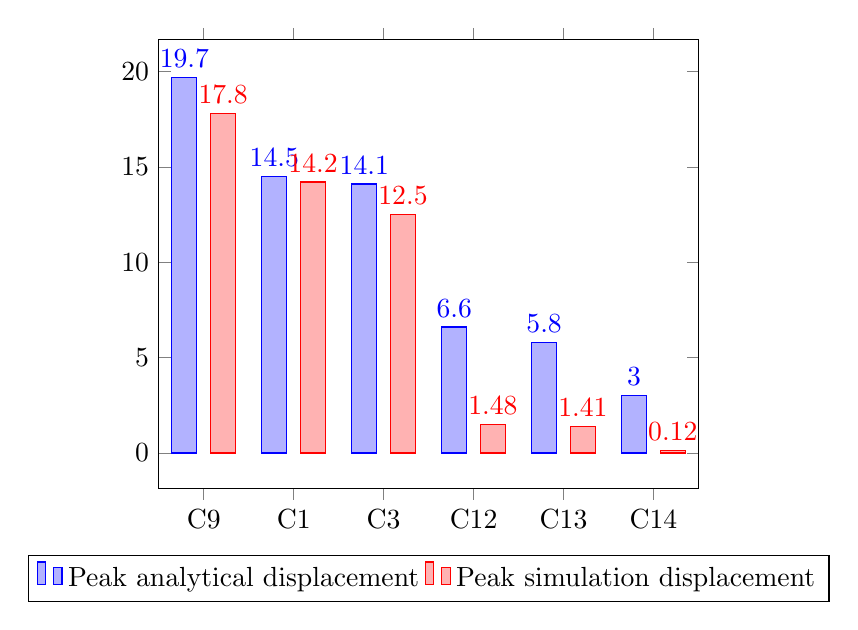
\begin{tikzpicture}
\begin{axis}[
    symbolic x coords={C9,C1,C3,C12,C13,C14},
    xtick=data,
    legend style={at={(0.5,-0.15)},
        anchor=north,legend columns=-1},
    ybar=5pt,% configures `bar shift'
    bar width=9pt,
    nodes near coords,
]
\addplot 
    coordinates {(C9, 19.7) (C1, 14.5) (C3, 14.1)   (C12,6.6) (C13,5.8) 
        (C14, 3.0) };
\addplot 
    coordinates {(C9, 17.8) (C1, 14.2) (C3, 12.5)  (C12,1.48) (C13,1.41)
         (C14,0.117) };
\legend{Peak analytical displacement,Peak simulation displacement}
\end{axis}
\end{tikzpicture}
\caption{Comparison between peak simulation result and peak analytical result}
\label{fig:comparisonpeaksimulationanalytical}
\end{figure}

To clearer illustrate the comparison of both peak results from simulation and analytical, Figure.\ref{fig:comparisonpeaksimulationanalytical} is created with rearranged x-axis order to make the descending trend more obvious. Please note all data sets except for C1 are valid for verification(C1 is used in creation of expression).

It can be seen that analytical results always keep a conservative margin above the simulation results. As expected, margins for C12,C13,C14 are bigger compared to C9,C1,C3 proofs that the analytical solution becomes more conservative if adopted to passenger train and high-speed train. What's more, the descending trend of analytical results follows the descending trend of simulation results perfectly regardless of train types. Thus considering these reasons, the analytical solution is sufficient for universal application on all train types.

\section{Finalizing the method for practical usage}

In practical usage, the speed that generates the highest peak response is unknown. Thus it is necessary to obtain the peak response for all speeds within the possible speed range. This is done by iterating the existing Matlab script with different speed. The increment in speed iteration is set in a way that ensures at least 1000 runs are done to guarantee precession. An example is illustrated as follows to show the usage on a real bridge project.

For an arch railway bridge located near Amsterdam, possessing following parameters:

$L = 255m$, $m = 5222e3kg$, $\mu = 2.0478e4 kg/m$, $EJ = 6.56e12Nm^2$

to test through a speed range of $1m/s - 30m/s$

Before beginning the calculation, make sure you have fog.m and Speedenvelop.m in your current working directory. By inputting following command in Matlab console, 

\texttt{Speedenvelop(6.56e12,255,2.0478e4,1,30,0.01)}


the envelop for displacement is generated and illustrated in Figure.\ref{fig:spedefEJ6560000000000L255min1max30mu20478.tikz}

\begin{figure}[h!]
\centering 
\setlength\figureheight{6cm} 
\setlength\figurewidth{6cm} 
% This file was created by matlab2tikz v0.4.7 (commit 29117077607177efe915cc01d961cced006239c8) running on MATLAB 8.3.
% Copyright (c) 2008--2014, Nico Schlmer <nico.schloemer@gmail.com>
% All rights reserved.
% Minimal pgfplots version: 1.3
% 
\begin{tikzpicture}

\begin{axis}[%
width=\figurewidth,
height=\figureheight,
scale only axis,
xmin=0,
xmax=30,
ymin=0.0075,
ymax=0.011,
title={SpeedEnvelop def from1 to30}
]
\addplot [color=blue,solid,forget plot]
  table[row sep=crcr]{%
1	0.00781568842060085\\
1.2	0.00840892567977264\\
1.4	0.0088768875903958\\
1.6	0.00925769529057003\\
1.8	0.00957910144655464\\
2	0.00982648840148397\\
2.2	0.0100372557099215\\
2.4	0.0102060089657038\\
2.6	0.010347841028453\\
2.8	0.0104753362289414\\
3	0.010566090236029\\
3.2	0.0106426943938749\\
3.4	0.0107156879259678\\
3.6	0.0107656368912521\\
3.8	0.0108134770961416\\
4	0.0108433829006734\\
4.2	0.0108762461970553\\
4.4	0.0109009754438711\\
4.6	0.0109137058875431\\
4.8	0.0109063964703489\\
5	0.0109283926778865\\
5.2	0.0109354115709882\\
5.4	0.010934364378216\\
5.6	0.010925358882146\\
5.8	0.0109155184260617\\
6	0.0109160952245694\\
6.2	0.0109022893020932\\
6.4	0.0108894990281659\\
6.6	0.0108791296950589\\
6.8	0.0108683159097076\\
7	0.0108485530748728\\
7.2	0.0108354499334163\\
7.4	0.0108143121429067\\
7.6	0.0107967054438007\\
7.8	0.0107826189027167\\
8	0.0107571129205081\\
8.2	0.0107450192698353\\
8.4	0.0107182431373167\\
8.6	0.0107081009100856\\
8.8	0.0106810097968274\\
9	0.0106647893596357\\
9.2	0.0106368269751327\\
9.4	0.0106244435627288\\
9.6	0.0105902161380316\\
9.8	0.0105787489298167\\
10	0.0105530497685275\\
10.2	0.0105311301588914\\
10.4	0.0105155111529359\\
10.6	0.0104818416711415\\
10.8	0.0104658192794055\\
11	0.0104515232844051\\
11.2	0.0104195968460413\\
11.4	0.0103992383576141\\
11.6	0.0103875827376142\\
11.8	0.0103585518798102\\
12	0.0103282987036047\\
12.2	0.0103183620397562\\
12.4	0.0103012474040927\\
12.6	0.0102668977746374\\
12.8	0.0102449204320541\\
13	0.0102354809790005\\
13.2	0.0102169579397151\\
13.4	0.0101865143682396\\
13.6	0.0101530378665145\\
13.8	0.0101488592884028\\
14	0.0101342026283539\\
14.2	0.0101129828210581\\
14.4	0.0100781640001081\\
14.6	0.010051230942275\\
14.8	0.0100463931273211\\
15	0.0100339102223161\\
15.2	0.0100154789040376\\
15.4	0.00998674150551577\\
15.6	0.00995047989615967\\
15.8	0.00993544019804088\\
16	0.00993088834100722\\
16.2	0.0099199018939231\\
16.4	0.00990104705345698\\
16.6	0.00987441551082942\\
16.8	0.00984237739719204\\
17	0.00980928040956712\\
17.2	0.0098093242438416\\
17.4	0.00980329783311577\\
17.6	0.00979122702961792\\
17.8	0.00977314390458511\\
18	0.00974908670711774\\
18.2	0.00972108217302529\\
18.4	0.0096776691907686\\
18.6	0.00966812567615805\\
18.8	0.0096672743699076\\
19	0.00966167442250244\\
19.2	0.00965133478148734\\
19.4	0.00963626874305325\\
19.6	0.00961649393213872\\
19.8	0.00959203227865456\\
20	0.00956290998985286\\
20.2	0.0095021185042862\\
20.4	0.00950695108828918\\
20.6	0.00950797086177456\\
20.8	0.00950518266938973\\
21	0.00949859410737403\\
21.2	0.00948821551471712\\
21.4	0.00947405996230233\\
21.6	0.00945635016311157\\
21.8	0.00943490732597904\\
22	0.00940971735699768\\
22.2	0.00931048059107463\\
22.4	0.00931929357671497\\
22.6	0.00932536783564737\\
22.8	0.00932827887006457\\
23	0.00932803971339443\\
23.2	0.00932466491318731\\
23.4	0.00931817052503146\\
23.6	0.00930857410555171\\
23.8	0.00929589470449585\\
24	0.0092803683442182\\
24.2	0.00926243390849551\\
24.4	0.0092414380792758\\
24.6	0.00916278336234724\\
24.8	0.00909609061802426\\
25	0.00910564521095271\\
25.2	0.00911382028447303\\
25.4	0.00911959836984988\\
25.6	0.00912274595493189\\
25.8	0.00912328389307619\\
26	0.00912136767440461\\
26.2	0.00911807810466714\\
26.4	0.00911219402539695\\
26.6	0.00910373969614448\\
26.8	0.0090927400294876\\
27	0.00907945686157787\\
27.2	0.00906461860626204\\
27.4	0.00904726523290454\\
27.6	0.00902380873477224\\
27.8	0.00882644457839617\\
28	0.00883996385182427\\
28.2	0.00885231633946435\\
28.4	0.00886244919403873\\
28.6	0.00887051931610704\\
28.8	0.00887784576510649\\
29	0.0088829756466977\\
29.2	0.00888593368675971\\
29.4	0.00888785865101469\\
29.6	0.00888798738354364\\
29.8	0.00888597303168551\\
30	0.00888235391855735\\
};
\end{axis}
\end{tikzpicture}% 
\caption{spedefEJ6560000000000L255min1max30mu20478} 
\label{fig:spedefEJ6560000000000L255min1max30mu20478.tikz} 
\end{figure}

The plot shows that the critical speed appears at approximately $5m/s$ and corresponding peak deflection response is approximately $11mm$. 

Since the relationship between end support rotation angle and mid-span deflection is widely known as:

$$ \varphi = \frac{3}{L}\cdot \delta_0  $$

and rotation is yielded as:

$$ \varphi = \frac{3}{255}\times 0.011 = 0.00013 $$

This value is much lower than the rotation value regulated in EN1991-2. See Section.\ref{sec:Transverse-deformations-and-vibrations} for criteria details.

Thus the conclusion can be made that this bridge is safe subjected to lateral dynamic load.

However, if encountering unfavourable peak result, a filter can be applied on the train speed to further cut off the peak response. In previous chapter it has been already be concluded that all resonance effects between train and bridge are wavelength phenomenon. In order to couple frequency with bridge's first natural bending frequency, the train needs to operate at a certain speed range. 

For example, assuming the train's wavelength is 20m-40m, including both axle repeat wavelength and kinematic wavelength. 

The natural frequency of the bridge in this example is 

$$ f_1 = \frac{\pi}{2l^2}\sqrt{\frac{EJ}{\mu}} = \frac{\pi}{2\times 255^2}\sqrt{\frac{6.56e12}{1.0478e4}} = 0.4Hz$$

so the possible resonance speed is obtained by multiplying wavelength range with natural frequency, yielding: $8m/s$ and $16m/s$

The maximum response in deflection is lowered to 1.05 mm. The filter is more effective if the natural frequency of the bridge is higher.

\chapter{Recommendations on improvement on Eurocode}


% \section{Another criterion proposed by J.J.Reber}
% A SNCB bridge, driver complains 

% To be used in combination with Sijian Deng's criterion.

% \section{Misc}

% Define eigen frequency and natural frequency

% Define how-to-do and what-to-do a dynamic analysis

\subsection{Add reference}
Please


\subsection{Improve criteria for lateral bridge dynamics}
Following sections provides several orientations for improving criteria for lateral bridge dynamics in terms of safety and serviceability of running stock.


\subsection{Requirements for traffic safety(horizontal)}
Requirements other than bridge first lateral frequency higher than 1.2Hz. Since there's no further requirements mentioned by Eurocode, following requirements are gathered from other European codes, eg. British standards, UIC leaflet, etc.

\begin{enumerate}[-]
    \item Requirements regarding traffic safety for vehicles
    \begin{enumerate}
        \item Guiding Force: \cite{code2005518} , \cite{en200714363} and\cite{cuadrado2008analysis} propose safty limitations against railway vehicle overturning. From\cite{en200714363} the maximum guiding force for a vehicle with a load per axle of 170kN(AVE) is 66kN per axle and 48kN per axle for a vehicle with a load per axle of 112kN(ICE2). For the R1 freight wagon(load per axle of 245kN), the maximum guiding force per axle is 78kN.
        \item Maximum lateral acceleration of the railway vehicle: proposed by \cite{13803}
    \end{enumerate}
    \item Requirements regarding safety for bridge\\
    \cite{EC0} A2.4.4.1(2): Horizontal transverse deflection(to ensure acceptable horizontal track radii) and horizontal rotation of a deck about a vertical axis at ends of a deck(to ensure acceptable acceptable horizontal track geometry and passenger comfort)
\end{enumerate}


\subsection{Requirements for traffic safety on derailment: Railway vehicle derailment mechanism and safety criteria}

Derailment mechanisms
\begin{enumerate}
    \item vehicle resonant response
    \item lateral instability
    \item vehicle overturning
    \item vertical wheel unloading
    \item flange climb
    \item rail roll-over
    \item track panel shift
    \item longitudinal train forces
\end{enumerate}

The four types of derailment: flange climb derailment, derailment caused by guage widening and rail roll-over, derailment caused by track panel shift, derailment cause by vehicle lateral instability have a common cause of high lateral force at the wheel-rail interface. According to \cite[Chapter 8, IV]{iwnicki2006handbook} any conditions that lead to high lateral forces or lead to lower the ability of the system to sustain the force should be corrected. 

\subsubsection{Flange climb derailment}
Wheel flange climb derailments are caused by wheels climbing onto the top of the railhead then further running over the rail. Wheel climb derailments generally occur in situations where the wheel experiences a high lateral force combined with circumstances where the vertical force is reduced on the flanging wheel. The high lateral force is usually induced by a large wheelset angle-of-attack. The vertical force on the flanging wheel can be reduced significantly on bogies having poor vertical wheel load equalisations, such as when negotiating rough track, large track twist, or when the car is experiencing roll resonances. 

\begin{figure}[h]
    \centering
    \includegraphics[width=0.4\textwidth]{forcesatflangecontactlocation.pdf}
    \caption{Forces at flange contact location. Extracted from \cite[Figure8.4]{iwnicki2006handbook}}
    \label{fig:forcesatflangecontactlocation}
\end{figure}

The criterion L/V ratio can be expressed as:

\begin{equation}
    \frac{L}{V}=\frac{\tan \delta -\frac{F_2}{F_3}}{1+\frac{F_2}{F_3}\tan \delta}
\end{equation}

Nadal's famous L/V ratio limiting criterion, given by Equation.\ref{eq:nadalcriterion}, was proposed for the saturated condition $F_2/F_3=\mu$

\begin{equation}\label{eq:nadalcriterion}
    \frac{L}{V}=\frac{\tan \delta - \mu}{1+ \mu \tan \delta}
\end{equation}

\subsubsection{Derailment caused by guage widening and rail rollover}
Derailments caused by guage widening usually involve a combination of wide gauges and large lateral rail defections(rail roll), as shown in Figure\ref{fig:gaugewideningderailment}. Large lateral forces from the wheels act to spread the rails in curves. Both rails may experience significant lateral translation and/or railhead roll, which often cause the nonflanging wheel to drop between rails.

\begin{figure}[h]
    \centering
    \includegraphics[width=0.8\textwidth]{gaugewideningderailment.pdf}
    \caption{Gauge widening derailment. Extracted from \cite[Figure8.18]{iwnicki2006handbook}}
    \label{fig:gaugewideningderailment}
\end{figure}

\paragraph{AAR Chapter XI rail roll criterion}
The AAR Chapter XI rail roll criterion is established by using the L/V ratio. The roll moment about the pivot point is given by,

\begin{equation}
    M=Vd-Lh
\end{equation}

under an equilibrium condition, just before the rail starts to roll, $M$ approaches to zero, then,

\begin{equation}
    \frac{L}{V}=\frac{d}{h}
\end{equation}

This L/V ratio is considered as the critical value to evaluate the risk of rail roll. When the L/V ratio is larger than the ratio of $d/h$, the risk of rail roll becomes high. The critical L/V ratio for rail roll can vary from above 0.6 for contact at the gauge side to approximately 0.2 when the contact position is at the far-field side based on the dimension of the rails. This is because the distance $d$ is reduced. Note that this L/V ratio is calculate assuming that neither the rail fasteners nor the torsional stiffness of the rail section provide any restraint.

\subsubsection{Derailment caused by track panel shift}
Track panel shift is the cumulative lateral displacement of the track panel, including rails, tie plates and ties, over the ballast, as shown in Figure\ref{fig:lateraltrackpanelshift}. A small shift of these components may not immediately cause the loss of guidance to bogies. However, as the situation gradually depreciates to a certain level, wheels could lose guidance and drop to the ground at some speed. The derailments caused by track panel usually result in one wheel falling between the rails and the other falling outside of the track.

\begin{figure}[h]
    \centering
    \includegraphics[width=0.8\textwidth]{lateraltrackpanelshift.pdf}
    \caption{Lateral track panel shift. Extracted from \cite[Figure8.27]{iwnicki2006handbook}}
    \label{fig:lateraltrackpanelshift}
\end{figure}

\paragraph{Panel shift criterion}
Researched by the French National Railways suggested that the limiting lateral axle load can be defined in a general expression for preventing excessive track panel shift:

\begin{equation}
    L_c = aV+b
\end{equation}

where $L_c$ is the critical lateral load and $V$ is the vertical axle load. \cite[Table 8.2]{iwnicki2006handbook} lists two groups of suggested valued of $a$ and $b$. It is possible that different values for $a$ and $b$ can be specified in different area.

\subsubsection{Derailment caused by vehicle lateral instability}
On tangent track, the wheelset generally oscillates around the track centre due to any vehicle and track irregularities, as shown in Figure\ref{fig:wheelsetoscillatesaroundthetrackcentre}. This movement occurs because vehicle and track are never absolutely smooth and symmetric. This self-centring capability of a wheelset is induced by the coned shape of the wheel tread. However, as speed is increased, if the whelset conicity is high, the lateral movement of wheelset, as well as the associated bogie and car body motion, can cause oscillations with large amplitude  and a well-defined wavelength. The lateral movements are limited only by the contact of the wheel flanges with the rail. This vehicle dynamic response is also termed as vehicle hunting, and can produce high lateral forces to damage track to cause derailments.

\begin{figure}[h]
    \centering
    \includegraphics[width=0.8\textwidth]{wheelsetoscillatesaroundthetrackcentre.pdf}
    \caption{Wheelset oscillates around the track centre. Extracted from \cite[Figure8.28]{iwnicki2006handbook}}
    \label{fig:wheelsetoscillatesaroundthetrackcentre}
\end{figure}

Derailment cause by vehicle hunting can have derailment mechanisms of all four types discussed in the previous sections. The high lateral force induced from hunting may cause wheel flange climbing on the rail, gauge widening, rail roll-over, track panel shift, or combinations of these. The safety concerns for this type of derailment, usually occurring at higher speeds, make it an important area of study.

Hunting predominantly occurs in empty or lightweight vehicles. The critical hunting speed is highly dependent on the vehicle/track characteristics. Investigation of the critical speed for such a system with nonlinearities is to examine the vehicle response to a disturbance using a numerical solution of the equations of motion.

\subsection{Requirements for traffic serviceability(horizontal)}

The criteria Comfort Indexes for assessing ride comfort in railway vehicles proposed in \cite{12299}. This standard describes a methodology for assessing ride comfort as a function of longitudinal, vertical and transverse accelerations.

Comfort Index indicates the percentage of passengers experimenting discomfort in a specific situation. These indexes can be computed via empiric formula given in the standard, which depend on variables such as lateral acceleration, rate of change of acceleration and rolling velocity. All these values are filtered with a moving average filter that eliminates small wavelength components. Using this methodology for the computed worst-case situations, the comfort indexes have been found excellent, therefore no passenger should feel uncomfortable.


%!TEX root = first try.tex

\chapter{Case study}

A case study to assess the feasibility of the methods/criteria developed in previous paragraphs by using both FEM software and methods/criteria. 


\chapter{Conclusion}

%Compare the result from different calculation method. Give conclusion based on the comparison result.

\begin{appendices}
\chapter{Frequency and wavelength data used in D181 DT 329}

\begin{table}[h]
    \centering
    \begin{tabular}{c|c|c|c}
    \hline
    \multirow{2}{*}{Freight train: Principle axle repeat patterns} & dist & \multicolumn{2}{c}{Speed} \\
    & m & 60 km/h & 100 km/h \\
    \hline
    wagon n axle 2 - wagon n+1 axle 1 & 4.00 & 4.17 & 6.94 \\
    wagon wheelbase & 9.00 & 1.85 & 3.09 \\
    wagon n axle m - wagon n+1 axle m & 13.0 & 1.28 & 2.14 \\
    wagon n axle m - wagon n+2 axle m & 26.0 & 0.64 & 1.07 \\
    \hline
    \multirow{2}{*}{Passenger train: Principle axle repeat patterns} & dist & \multicolumn{2}{c}{Speed} \\
    & m & 160 km/h & 200 km/h \\
    \hline
    coach n axle 1 - 2, and coach n axle 3 - 4 & 2.56 & 17.36 & 21.70 \\
    coach n axle m - coach n+1 axle m & 26.4 & 1.68 & 2.10 \\
    coach n axle m - coach n+2 axle m & 52.8 & 0.84 & 1.05 \\
    \hline
    \multirow{2}{*}{ETR 500 train: Principle axle repeat patterns} & dist & \multicolumn{2}{c}{Speed} \\
    & m & 300 km/h & 350 km/h \\
    \hline
    coach n axle 1 - 2 and coach n axle 3 - 4 & 3.0 & 27.78 & 32.41 \\
    coach n axle m - coach n+1 axle m & 26.1 & 3.19 & 3.72 \\
    coach n axle m - coach n+2 axle m & 52.2 & 1.60 & 1.86 \\
    coach n axle m - coach n+3 axle m & 69.3 & 1.20 & 1.40 \\
    \hline
    \end{tabular}
    \caption{Axle repeat patterns and typical frequencies. Extracted from \cite[Appendix C]{d181dt329}}
    \label{tab:329axlerepeat}
\end{table}

\begin{table}[h]
    \centering
    \begin{tabular}{c|c|c|c}
    \hline
    Kinematic wavelength, m & Freight train & Passenger train & ETR500 train \\
    \hline
    Locomotive & 39 - 45 & 32 - 38 & 39 - 45 \\
    Coach/wagon & 24 - 39 & 34 - 38 & 36 - 40 \\
    \hline
    \end{tabular}
    \caption{Kinematic wavelength ranges per vehicle, with BR P1 profiles. Extracted from \cite[Appendix C]{d181dt329}}
    \label{tab:329kinematicwavelength}
\end{table}

\chapter{Speeds which do not require dynamic compatibility checks} \label{app:speedsafe}

\begin{figure}[h]
    \centering
    \includegraphics[width=0.7\textwidth]{speedsafe.pdf}
    \caption{Speed limit (in km/h) in relationship Line Category/Locomotive Class and vehicle type. Extract from \cite[Appendix F]{EC15528}}
\end{figure}

\chapter{MU-Groups and MU-Classes}\label{app:mu}

\section{Definition}
Multiple units can be grouped according to type of traffic service(high speed - long distance, intercity - regional and commuter/suburban) or to the kind of running gear (conventional bogies, articulated bogies and single axles).


In some cases due to potential excessive dynamic load effects in bridge line category checks are not sufficient to demonstrate compatibility. To minimise the need for undertaking a dynamic check of individual trains, several typical and wide spread MU-designs have been grouped in MU-classes. For these groups of vehicles, load models covering the specified design parameter ranges have been developed to allow the efficient dynamic analysis of bridges. For practical reasons, the number of MU classes was limited and for trains outside the range of parameters covered, the process of checking an individual train existing at the time of publication of this standard as state of the art shall be used.

Each MU-class is defined by:

\begin{enumerate}[-]
\item ranges of train parameters covered and;
\item a corresponding load model for carrying out dynamic checks on bridges.
\end{enumerate}

Each MU-Group comprises of serveral MU-Classes. Table

\begin{table}[h]
    \centering
    \begin{tabular}{c|c}
        \hline
        MU-Group & MU-Class\\
        \hline
        \multirow{2}{*}{conventional bogie(CB)} & $CB_1$ \\
        & $CB_2$ \\
        \hline
        \multirow{4}{*}{articulated bogie(AB)} & $AB_1$ \\
        & $AB_2$ \\
        & $AB_3$ \\
        & $AB_4$ \\
        \hline
        \multirow{2}{*}{single axle(SA)} & $SA_1$ \\
        & $SA_2$ \\
        \hline
    \end{tabular}
    \caption{Relationship MU-groups - MU-classes}
    \label{tab:MU}
\end{table} 

\begin{figure}[h]
\centering
\includegraphics[width=0.8\textwidth]{trainparameters.pdf}
\caption{Train parameters related to MU-Groups. Extracted from \cite[Annex C]{EC15528}}
\label{fig:trainparameters}
\end{figure}

\begin{table}[h]
    \centering
    \begin{tabular}{c|c|c}
    \hline
    Name & Parameter & Unit \\
    $2a^*$ & Bogie spacing between pivot centres within a vehicle & m \\
    $2a^+$ & Axle spacing in bogie & m \\
    $u1+u2$ & Bogie spacing between pivot centres of adjacent vehicles & m \\
    $u3$ & Overhang of end coaches & m \\
    L\_Coa & Coach length & m \\
    No\_Coa & Number of coaches within an unit & - \\
    No\_Units & Number of units within a train & - \\
    \hline
    \end{tabular}
    \caption{Explanation of train parameters. Extracted from \cite[Annex C]{EC15528}}
    \label{tab:explanationtrainparameters}
\end{table}

\subsection{Train parameters of MU-Class CB\_1}

\begin{table}[h]
    \centering
    \begin{tabular}{c|c}
    \hline
    max No\_Units & 2 \\
    max No\_Coa & 8 \\
    L\_Coa & $23.8m \leq L\_Coa \leq 25.3m $ \\
    $2a^*$ & $16.8m \leq 2a^* \leq 18.0m $ \\
    $2a^+$ & $2m \leq 2a^+ \leq 3m $ \\
    $(u1+u2)$ & $7.0m \leq (u1+u2) \leq 7.6m $ \\
    $u3$ & $4m \leq u3 \leq 6m $ \\
    \hline
    \end{tabular}
    \caption{Train parameters for conformity with MU-Class CB\_1}
    \label{tab:CB1}
\end{table}

\subsection{Train parameters of MU-Class CB\_2}

\begin{table}[h]
    \centering
    \begin{tabular}{c|c}
    \hline
    max No\_Units & 2 \\
    max No\_Coa & 7 \\
    L\_Coa & $ 25.3 m \leq L\_Coa \leq 27.5 m $ \\
    $2a^*$ & $ 18.0 m \leq 2a^* \leq 19.5 m $ \\
    $2a^+$ & $ 2 m \leq 2a^+ \leq 3m $ \\
    $(u1+u2)$ & $7.2m \leq (u1+u2) \leq 8.0 m $ \\
    $u3$ & $4m \leq u3 \leq 6m $ \\
    \hline
    \end{tabular}
    \caption{Train parameters for conformity with MU-Class CB\_2}
    \label{tab:CB2}
\end{table}


\subsection{Train parameters of MU-Class AB\_1}

\begin{table}[h]
    \centering
    \begin{tabular}{c|c}
    \hline
    max No\_Units & 4 \\
    max No\_Coa & 5 \\
    $2a^*$ & $ 14.9 m \leq 2a^* \leq 16.0 m $ \\
    $2a^+$ & $ 2 m \leq 2a^+ \leq 3m $ \\
    $u3$ & $3m \leq u3 \leq 5.5m $ \\
    \hline
    \end{tabular}
    \caption{Train parameters for conformity with MU-Class AB\_1}
    \label{tab:AB1}
\end{table}

\subsection{Train parameters of MU-Class AB\_2}

\begin{table}[h]
    \centering
    \begin{tabular}{c|c}
    \hline
    max No\_Units & 4 \\
    max No\_Coa & 5 \\
    $2a^*$ & $ 18.8 m \leq 2a^* \leq 19.5 m $ \\
    $2a^+$ & $ 2 m \leq 2a^+ \leq 3m $ \\
    $u3$ & $3m \leq u3 \leq 5.5m $ \\
    \hline
    \end{tabular}
    \caption{Train parameters for conformity with MU-Class AB\_2}
    \label{tab:AB2}
\end{table}

\subsection{Train parameters of MU-Class AB\_3}

\begin{table}[h]
    \centering
    \begin{tabular}{c|c}
    \hline
    max No\_Units & 2 \\
    max No\_Coa & 11 \\
    $2a^*$ & $ 17.0 m \leq 2a^* \leq 17.5 m $ \\
    $2a^+$ & $ 2 m \leq 2a^+ \leq 3m $ \\
    $u3$ & $4.5m \leq u3 \leq 5.7m $ \\
    \hline
    \end{tabular}
    \caption{Train parameters for conformity with MU-Class AB\_3}
    \label{tab:AB3}
\end{table}

\subsection{Train parameters of MU-Class AB\_4}

\begin{table}[h]
    \centering
    \begin{tabular}{c|c}
    \hline
    max No\_Units & 2 \\
    max No\_Coa & 10 \\
    $2a^*$ & $ 18.7 m \leq 2a^* \leq 19.2 m $ \\
    $2a^+$ & $ 2 m \leq 2a^+ \leq 3m $ \\
    $u3$ & $4.3m \leq u3 \leq 5.3m $ \\
    \hline
    \end{tabular}
    \caption{Train parameters for conformity with MU-Class AB\_4}
    \label{tab:AB4}
\end{table}

\subsection{Train parameters of MU-Class SA\_1}

\begin{table}[h]
    \centering
    \begin{tabular}{c|c}
    \hline
    max No\_Units & 3 \\
    max No\_Coa & 10 \\
    $2a^*$ & $ 9.2 m \leq 2a^* \leq 9.8 m $ \\
    $u3$ & $4.25m \leq u3 \leq 6.25m $ \\
    \hline
    \end{tabular}
    \caption{Train parameters for conformity with MU-Class SA\_1}
    \label{tab:SA1}
\end{table}

\subsection{Train parameters of MU-Class SA\_2}

\begin{table}[h]
    \centering
    \begin{tabular}{c|c}
    \hline
    max No\_Units & 2 \\
    max No\_Coa & 14 \\
    $2a^*$ & $ 12.8 m \leq 2a^* \leq 13.5 m $ \\
    $u3$ & $4.25m \leq u3 \leq 6.25m $ \\
    \hline
    \end{tabular}
    \caption{Train parameters for conformity with MU-Class SA\_1}
    \label{tab:SA1}
\end{table}

\end{appendices}


\printbibliography 
\end{document}